  % -*- Mode:TeX -*-
%% This file simply contains the commands that actually generate the table of
%% contents and lists of figures and tables.  You can omit any or all of
%% these files by simply taking out the appropriate command.  For more
%% information on these files, see appendix C.3.3 of the LaTeX manual.
{%
\setlength{\parskip}{\initialparskip}%
\setlength{\parindent}{\initialparindent}%
\setlength{\topsep}{\initialtopsep}%
\setlength{\partopsep}{\initialpartopsep}%
\tableofcontents
%\newpage
%\listoffigures
%\newpage
%\listoftables
}%

\minortodo{decide on chapter/section capitalization and be consistent}
\minortodo{figure out if regression stats should be included, and, if so, how to calculate them}
\minortodo{make sure all appendices are at the very end, so we keep a linear progression}
\todo{update rewriting paper chapter with camera-ready file before editing}
\minortodo{add labels on every section, ensure no duplicate labels}
\minortodo{Decide whether or not to use contractions (less formal, but okay for thesis if I make a conscious decision)}
\minortodo{be consistent about $\lambda x. body$ vs.~$\lambda x, body$ (note that Coq only accepts the latter)}
\minortodo{move any citations which point at people.csail.mit.edu to point at a github.io version, and move my personal website there}
\minortodo{maybe include all code in an appendix?}
\minortodo{be consistent about function extensionality vs functional extensionality}
\minortodo{include github code links for contributions}
\part{Introduction}\label{part:introduction}
\begin{quote}
  Testing shows the presence, not the absence of bugs
\end{quote}
\begin{flushright}
  --- Edsger Wybe Dijkstra, 1969~\cite{naur1969software}
\end{flushright}

\begin{quote}
  If you blindly optimize without profiling, you will likely waste your time on the 99\% of code that isn't actually a performance bottleneck and miss the 1\% that is.
\end{quote}
\begin{flushright}
  --- Charles E.~Leiserson~\cite{Profiling2020Leiserson}
\end{flushright}

\begin{quote}
  premature optimization is the root of all evil
\end{quote}
\begin{flushright}
  --- Donald E.~Knuth~\cite[p.~671]{KnuthPrematureOptimization}
\end{flushright}

\chapter{Introduction}\label{ch:intro}

\section{Introduction}\label{sec:intro:intro}

%\paragraph{Paragraph 1: Orient the reader to very broad things} Software w/o bugs via formal methods
As our world comes to rely more and more on large and complex software, the impact of bugs in our code grows ever more severe.
Bugs in the software of the Therac-25, a radiation-therapy machine, killed three people and injured at least three more between 1985 and 1987 by delivering potentially leathal doses of radiation.~\cite{Therac}
\todo{Yes: Include more text from the following (at least three examples in this paragraph)}
\todo{do I need a better citation than wikipedia? Answer: Yes, find a primary source, especially as the citation is so early}
\todo{should I mention the pricing bug on amazon? https://www.usatoday.com/story/tech/2019/07/19/amazon-prime-day-error-sold-13-000-camera-equipment-94-report/1775314001/, https://www.theguardian.com/money/2014/dec/14/amazon-glitch-prices-penny-repricerexpress, http://www.michaeleisen.org/blog/?p=358}
More recently, unforseen edge-cases in DAO smart-contracts nearly cost investors over 40 million USD.~\cite{DAO2018Guecluetuerk}
\todo{should I mention anything else? the pentium bug costing Intel \$475 million? http://top-100s.blogspot.com/2009/05/10-most-expensive-software-blunders.html, \$500 million Ariane Rocket disaster? , https://www.olenick.com/blog/articles/infamous-software-bugs-fdiv-bug}
\todo{should I pull from https://xavierleroy.org/talks/Milner-award-lecture.pdf? ``Fiat-Chrysler recalled 1.5 M vehicles for software update.''}
\todo{\textcite{zhivich2009real}}

While testing of various kinds is widely used to catch bugs, it's quite costly \todoask{should I email Xavier Leroy and ask if he has references on how much the airline industry spends on testing?} and does not guarantee a lack of bugs.
In some adversarial contexts, random testing cannot hope to eliminate all bugs.
For example, some bugs in cryptographic code only occur in as few as 19 out of $2^{255}$ cases.~\cite{curve25519-donna-commit-correct-bounds}
Suppose you wanted to catch this bug in a ``modest'' twenty years of continuous random testing.
You'd need to have over a thousand times as many computers as there are atoms in the solar system!
% https://www.wolframalpha.com/input/?i=%282%5E255%2F19+*+529812+%2F+%285+ghz%29+%2F+%2820+years%29+%2F+%28atoms+in+the+solar+system%29%29+*+1+atom = 533260
% (2^255/19 * 529812 / (5 ghz) / (20 years) / (atoms in the solar system)) * 1 atom

%\paragraph{Paragraph 2: Success of foundational tools}
One appealing solution to this problem is to \emph{prove} critical software correct.
The idea is that if we can write down in formal mathematical language what we'd like our software to do, then we can try to prove that the code that actually runs behaves in the same way that the math specifies.
Ideally, the specification will be relatively simple, and much easier to trust, than the millions of lines of code making up the software we use every day.

While proofs of algorithms tend to be done with pen-and-paper (consider the ubiquitous proofs that various sorting algorithms are correct in introductory algorithms classes), proofs of actual code are much harder.
For reasons of performance, historical accident, interfacing with real users, or otherwise, code in the real-world tends to be much more complicated than code in an algorithms textbook.
Proofs of code-correctness thus tend to be filled with tedious case-analysis with only sparse mathematical insights, and attempts to create and check these proofs by hand are subject to the same issues of human falibility as writing the programs in the first place.

%\todo{transition to foundational tools}
%\todo{explain how foundational tools like Coq are already useful}
Enter machine-checked proofs.
Foundational tools which allow users to write down theorems and proofs to be checked by machine free the proof author from error-prone case analysis; the computer will check that no cases were missed.
Although you can never gain complete confidence in your software---the layer underneath may be untrustworthy in ways you cannot see~\cite{Reflections1984Thompson}, you can never prove that the mathematical system you're working in is correct~\cite{sep-goedel-incompleteness}, and most proof-checkers are not yet themselves proven correct---machine-checked proofs allow a drastic reduction in how much code needs to be trusted.
Rather than trusting the millions of lines of code of the software being verified, you only need to trust the specifications of the software, and the likely-much-smaller codebase of the proof checker.
Furthermore, it's very unlikely that bugs in the proof checker will overlap with bugs in the proof in just the right way to allow bugs only in one particular piece of software to slip through.
Said another way, we no longer need to write tests for every piece of software separately; writing tests for the proof-checker helps eliminate bugs in \emph{all} software proven by that checker.

%\paragraph{Paragraph 3: performance of tools is important and non-trivial, and what we're doing here is explaining / demonstrating how and why it's non-trivial, and how to fix nontrivial performance issues}
We come now to the main thrust of this thesis.
Tools for machine-checked proofs have already had many successes, in both software verification and traditional mathematics proof formalization, from compilers~\cite{Compcert} to microkernels~\cite{seL4SOSP09} to webservers~\cite{Network2015Chlipala} to cryptography code~\cite{FiatCryptoSP19}, from the Four-Color Theorem~\cite{gonthier2008formal} to the Odd-Order Theorem~\cite{gonthier2013machine} to Homotopy Type Theory~\cite{HoTTBook}.
While compiler performance---both the time it takes to compile code and the time it takes to run the generated code---has long been an active field of study~\cite{CC++Performance2017,georges2007statistically,mytkowicz-wrong-data}\todo{find more citiations here}, to our knowledge there is no extant body of work systematically investigating the performance of proof assistants, nor even any work primarily focused on the problem of proof assistant performance writ large.
\todo{integrate stuff from \textcite{Efficiency1994Boulton} such as ``For example, much of the research in the field of automated reasoning is concerned with producing proofs more efficiently''}
\todo{Related to this is work on sound interfaces to external tools, also an enduring topic: \textcite{TrustedSlind}}

\todo{work on this paragraph}
Why is this problem worthy of study?
This thesis argues that the problem of \emph{compile-time performance} or \emph{proof-checking performance} is both significantly different from the problem of performance of more typical programs in industry and that it is nontrivial.
While many papers mention performance, obliquely or otherwise, and some are even driven by performance concerns of a particular algorithm or part of the system,~\cites[p.~1382]{gonthier2008formal}{Efficiency1994Boulton}{Proving2005Benjamin}{Idris2Faster2020Brady}{Recognizing1989Benanav}{mechanical1990Pierce}{CelikETAL17iCoq}{PalmskogETAL18piCoq}{Gregoire-Leroy-02}{thesis-nogin}{Idris2Faster2020Brady}, we have not found any that investigate the performance problems that arise \emph{asymptotically}, when proof assistants are used to verify programs at large scale.
% ``While we tackled this project mainly to explore the capabilities of a modern formal proof system—at first, to benchmark speed—'' - gonthier2008formal
% ``We present a new implementation of a reflexive tactic whichsolves equalities in a ring structure inside the Coq system.The efficiencyis improved to a point that we can now prove equalities that were previ-ously beyond reach.'' - Proving2005Benjamin

Unlike many other performance domains, in our experience, the time it takes to check proofs as we scale the size of the input is almost always super-linear---quadratic at best, commonly cubic or exponential, ocassionally even worse.
Empirially, this might look like a proof script that checks in tens of seconds on the smallest of toy examples; takes about a minute on the smallest real-world example, which might be twice the size of the toy example; takes twenty hours to generate and check the proof of an example only twice that size; and, on a (perhaps not-quite-realistic) example twice the size of the twenty-hour example, the script might not finish within a year, or even a thousand years---see \autoref{sec:fiat-crypto-codegen-numbers} for more details.
In just three doublings of input size, we might go from tens of seconds to thousands of years.
Moreover, this is not an isolated experience in proof assistants; this sort of performance behavior is \emph{typical}.

Drawing experience from case studies in category theory~\cite{category-coq-experience}, parsers~\cite{jgross-masters-thesis}, and generation of low-level cryptographic code~\cite{FiatCryptoSP19}, we investigate and seek to explicate a broad swath of performance issues and bottlenecks.
While we propose some design principles for avoiding these performance issues in \autoref{part:design} and present a research prototype of a tool and methodology for achieving acceptable performance at scale in \autoref{part:rewriting}---and we claim both of these are original contributions of this PhD\todo{how to write PhD in text?  with periods? not?}---the story this thesis aims to tell is that in order for proof assistants to scale to industrial uses, \emph{we must get the basics of asymptotic performance right}.

\subsection{What are proof assistants?}\label{sec:intro:history}
\todo{is it Nuprl or NuPRL? make sure to be consistent}
%{The structure of this section:}
%\begin{itemize}
%\item {how the first proof assistants worked}
%\item {subsubsection on LCF approach, and how that lets you prove things}
%\item {paragraph on descendents of LCF, dependently typed and not; foreshadow how proof checking as typechecking works with a single sentence or so}
%\item {very brief paragraph on other proof assistants, also mention survey papers}
%\item {paragraph on successes of proof assistants}
%\end{itemize}
%
Before diving into the details of performance bottlenecks and solutions, we review the history of formal verification and proof assistants to bring the reader up to speed on the context of our work and investigation.
\todo{Maybe say something about the purpose of this section: simultaneously let people know that there's been a lot of thought and effort, let people know about success stories (because it possibly hasn't touched them, and hasn't been adopted mainstream), (and also a bit about how the proof assistants might actually check the proofs)}
\todo{cite the following in chronological order, maybe}
While we intend to cover a wide swath of the history and development in this subsection, far more detailed descriptions can be found in the literature~\cites{ringer2020qed,Proof2009Geuvers,History2014Harrison,CoqArtForward2013Huet,Brief2019Darbari,davis2001early,Matuszewski05mizar:the,Automath2002Kamareddine,Milestones2019Moore,Automation2013Moore,LCF2000Gordon,LCF2019Paulson,Logical2002Pfenning}[Related Work]{nuprl}.
\textcite[ch.~4]{ringer2020qed} has a particularly clear presentation which was invaluable in assembling this section.

Formal verification can be traced back to the early 1950's.~\cite{Brief2019Darbari}
The first formally verified proof, in some sense, achieved in 1954, was of the theorem that the sum of two even numbers is even.~\cite{davis2001early}
The ``proof'' was an implementation in a vacuum-tube computer of the algorithm of \textcite{Uber1929Presburger}, which could decide, for any first order formula of natural number arithmetic, whether the formula represented a true theorem or a false one;
by implementing this algorithm and verifying that it returns ``true'' on a formula such as $\forall a\ b\ x\ y,\ \exists z,\ a = x + x \to b = y + y \to a + b = z + z$, the machine can be said to prove that this formula is true.

While complete decision procedures exist for arithmetic, propositional logic (the fragment of logic without quantifiers, i.e., consisting only of $\to$, $\wedge$, $\vee$, $\neg$, and $\iff$), and elementary geometry, there is no complete decision procedure for first-order logic, which allows predicates, as well as universal and existential quantification over objects~\cite{davis2001early}.
In fact, first-order logic is sufficiently expressive to encode systems that reason about themselves, such as Peano arithmetic, and G\"odel's incompleteness theorem proves that there must be some statements which are neither provably true nor provably false.
In fact, we cannot even decide which statements are undecidable~\cite{Are2011Makholm}!

This incompleteness, however, does not sink the project of automated proof search.
Consider, for example, the very simple program that merely lists out all possible proofs in a given logical system, halting only when it has found either a proof or a disproof of a given statement.
While this procedure will run forever on statements which are neither provably true nor provably false, it will in fact be able to output proofs for all provable statements.
This procedure, however, is uselessly slow.

More efficient procedures for proof search exist, however.
\todo{Should I cite \textcite{Computing1960Davis}, which was an earlier form of the resolution rule that proved infeasible?}
Early systems such as the Stanford Pascal Verifier~\cite{luckham1979stanford} and Stanford Resolution Prover were based on what is now known as Robinson's resolution rule~\cite{Machine1965Robinson}, which, when coupled with syntactic unification, resulted in tolerable performance on sufficiently simple problems~\cite{davis2001early,Brief2019Darbari}.
A particularly clear description of the resolution method can be found in \textcite[pp.~17--18]{Metamathematics1994Shankar}.
In the 1960's, all 400-or-so theorems of Whitehead and Russell's \emph{Principia Mathematica} were automatically proven by the same program~\cite[p.~9]{davis2001early}.
However, as the author himself notes, this was only feasible because all of the theorems could be expressed in a way where all universal qunatifiers came first, followed by all existential quantifiers, followed by a formula without any quantifiers.

In the early 1970's, Boyer and Moore began work on theorem provers which could work with higher-order principles such as mathematical induction~\cite[p.~6]{Automation2013Moore}.
This work resulted in a family of theorem provers, collectively known as the Boyer--Moore theorem provers, which includes the first seriously successful automated theorem provers~\cites[p.~8]{Automation2013Moore}{Brief2019Darbari}.
They developed the Edinburgh Pure LISP Theorem Prover, Thm, and later Nqthm~\cites[p.~8]{Automation2013Moore}{Nqthm,wiki:Nqthm}, the last of which came to be known as \emph{the} Boyer--Moore theorem prover.
Nqthm has been used to formalize and verify G\"odel's first incompleteness theorem in 1986~\cites{Metamathematics1994Shankar}[p.~29]{Milestones2019Moore}, to verify the implementation of an assembler and linker~\cite{moore2007piton} as well as a number of FORTRAN programs, and to formally prove the invertibility of RSA encryption, the undecidability of the halting problem, Gauss' law of quadratic reciprocity~\cite[pp.~28--29]{Milestones2019Moore}.
Nqthm later evolved into ACL2~\cite{Milestones2019Moore,ACL2Applications,ACL2}, which has been used, among other things, to verify a Motorola digital signal processor, the floating-point arithmetic unit in AMD chips, and some x86 machine code programs~\cite[p.~2]{Milestones2019Moore}.
% More details on the assembler and linker (Piton) at \url{https://www.cs.utexas.edu/~moore/best-ideas/piton/index.html}
% Also Computational Logic Inc.~which used Nqthm, \url{http://www.computationallogic.com/}

In 1967, at around the same time that Robinson published his resolution principle, N.~G.~de Bruijn developed the Automath system~\cite{Automath2002Kamareddine,Survey1994deBruijn,mathematical1970Bruijn,wiki:AutoMath}.
Unlike the Boyer--Moore theorem provers, Automath checked the validity of sequences of human-generated proof steps, and hence was more of a proof checker or proof assistant than an automated theorem prover~\cite{ringer2020qed}.
Automath is notable for being the first system to represent both theorems and proofs in the same formal system, reducing the problem of proof checking to that of type checking~\cite{ringer2020qed} by exploiting what came to be known as the Curry--Howard correspondence~\cite{Automath2002Kamareddine}; we will discuss this more in \autoref{sec:why-how-dependent-types}.
The legacy of Automath also includes de Bruijn indices, a method for encoding function arguments which we describe in \autoref{sec:binders:de-bruijn}, dependent types, which we explain in \autoref{sec:why-how-dependent-types}, and the \emph{de Bruijn principle}---stating that proof checkers should be as small and as simple as possible---which we discuss in \autoref{sec:debruijn-criterion}~\cite{ringer2020qed,Automath2002Kamareddine}.
We are deferring the explanation of these important concepts for the time being because, unlike the methods of theorem proving described above, these methods are at the heart of Coq, the primary theorem prover used in this thesis, as well as proof assistants like it.
One notable accomplishment in the Automath system was the translation and checking of the entirety of Edmund Landau's \emph{Foundations of Analysis} in the early 1970s~\cite{Automath2002Kamareddine}.

Almost at the same time as Boyer and Moore were working on their theorem provers in Edinburgh, Scotland, Milner developed the LCF theorem prover at Stanford in 1972~\cite[p.~1]{LCF2000Gordon}.
Written as an interactive proof checker based on Dana Scott's 1969 logic for computable functions (which LCF abbreviates), LCF was designed to allow users to interactively reason about functional programs~\cite[p.~1]{LCF2000Gordon}.
In 1973, Milner moved to Edinburgh and designed Edinburgh LCF, the successor to Stanford LCF.
This new version of LCF was designed to work around two deficiencies of its predecessor: theorem proving was limited by available memory for storing proof objects, and the fixed set of functions for building proofs could not be easily extended.
The first of these was solved by what is now called ``the LCF approach'': by representing proofs with an abstract \texttt{thm} type, whose API only permitted valid rules of inference, proofs did not have to be carried around in memory~\cites[pp.~1--2]{LCF2000Gordon}{harrison2001lcf}.
In order to support abstract data types, Milner et al.~invented the language ML (short for ``Meta Language'')~\cite[p.~2]{LCF2000Gordon}, the precursor to Caml and later OCaml.
The second issue---ease of extensibility---was also addressed by the design of ML~\cite[p.~2]{LCF2000Gordon}.
By combining an abstract, opaque, trusted API for building terms with a functional programming language, users were granted the ability to combine the basic proof steps into ``tactics''.
Tactics were functions that took in a goal, that is, a formula to be proven, and returned a list of remeaining subgoals, together with a function that would take in proofs of those subgoals and turn them into a proof of the overall theorem.
An example: a tactic for proving conjunctions might, upon being asked to prove $A \wedge B$, return the two-element list of subgoals $[A, B]$ together with a function that, when given a proof of $A$ and a proof of $B$ (i.e., when given two \texttt{thm} objects, the first of which proves $A$ and the second of which proves $B$), combines them with a primitive conjunction rule to produce a proof object justifying $A \wedge B$.
\todo{Do I need to say more about LCF?}
\todo{Do I need to say more about tactics?}

\todo{How should I summarize this into relevant paragraphs???}
\begin{quote}
Gérard Huet started working on automatic theorem proving in 1970, using LISP to implement the SAM prover for first-order logic with equality.
At the time, the state of the art was to translate all logical propositions into lists (conjunctions) of lists (disjunctions) of literals (signed atomic formulas), quantification being replaced by Skolem functions.
In this representation deduction was reduced to a principle of pairing complementary atomic formulas modulo instantiation (so-called resolution with principal unifiers).
Equalities gave rise to unidirectional rewritings, again modulo unification.
Rewriting order was determined in an ad hoc way and there was no insurance that the process would converge, or whether it was complete.
Provers were black boxes that generated scores of unreadable logical consequences.
The standard working technique was to enter your conjecture and wait until the computer's memory was full.
Only in exceptionally trivial cases was there an answer worth anything.
This catastrophic situation was not recognized as such, it was understood as a necessary evil, blamed on the incompleteness theorems.
Nevertheless, complexity studies would soon show that even in decidable areas, such as propositional logic, automatic theorem proving was doomed to run into a combinatorial wall.

A decisive breakthrough came in the 1970s with the implementation of a  systematic methodology to use termination orders to guide rewriting, starting from the founding paper of Knuth and Bendix.
The KB software, implemented in 1980 by Jean-Marie Hullot and Gérard Huet, could be used to automate in a natural way decision and semi-decision procedures for algebraic structures.
At the same time, the domain of proofs by induction was also making steady progress, most notably with the NQTHM/ACL of Boyer and Moore.
Another significant step had been the generalization of the resolution technique to higher-order logic, using a unification algorithm for the theory of simple types, designed by Gérard Huet back in 1972.
This algorithm was consistent with a general approach to unification in an equational theory, worked out independently by Gordon Plotkin.

At the same time, logicians (Dana Scott) and theoretical computer scientists (Gordon Plotkin, Gilles Kahn, Gérard Berry) were charting a logical theory of computable functions (computational domains) together with an effectively usable axiomatization (computational induction) to define the semantics of programming languages.
There was hope of using this theory to address rigorously the problem of designing trustworthy software using formal methods.
The validity of a program with respect to its logical specifications could be expressed as a theorem in a mathematical theory that described the data and control structures used by the algorithm.
These ideas were set to work most notably by Robin Milner's team at Edinburgh University, who implemented the LCF system around 1980.
The salient feature of this system was its use of proof tactics that could be programmed in a meta-language (ML).
The formulas were not reduced to undecipherable clauses and users could use their intuition and knowledge of the subject matter to guide the system within proofs that mixed automatic steps (combining predefined and specific \emph{tactics} that users could program in the ML language) and easily understandable manual steps.

Another line of investigation was explored by the philosopher Per Martin-Löf, starting from the constructive foundations of mathematics initially proposed by Brouwer and extended notably by Bishop's development of constructive analysis.
Martin-Löf's Intuitionistic Theory of Types, designed at the beginning of the 1980s, provided an elegant and general framework for the constructive axiomatization of mathematical structures, well suited to serve as a foundation for functional programming.
This direction was seriously pursued by Bob Constable at Cornell University who undertook the implementation of the NuPRL software for the design of software from formal proofs, as well as by the ``Programming methodology'' team headed by Bengt Nordström at Chalmers University in Gothenburg.

All this research relied on the λ-calculus notation, initially designed by the logician Alonzo Church, in its pure version as a language to define recursive functionals, and in its typed version as a higher-order predicate calculus (the theory of simple types, a simpler alternative for meta-mathematics to the system originally used by Whitehead and Russell in \emph{Principia Mathematica}).
Furthermore, the λ-calculus could also be used to represent proofs in a natural deduction format, thus yielding the famous ``Curry-Howard correspondence,'' which expresses an isomorphism between proof structures and functional spaces.
These two aspects of the λ-calculus were actually used in the Automath system for the representation of mathematics, designed by Niklaus de Bruijn in Eindhoven during the 1970s.
In this system, the types of λ-expressions were no longer simple hierarchical layers of functional spaces.
Instead they were actually λ-expressions that could express the dependence of a functional term's result type on the value of its argument---in analogy with the extension of propositional calculus to first-order predicate calculus, where predicates take as arguments terms that represent elements of the carrier domain.

λ-calculus was indeed the main tool in proof theory.
In 1970, Jean-Yves Girard proved the consistency of Analysis through a proof of termination for a polymorphic λ-calculus called system $F$.
This system could be generalized to a calculus $Fω$ with polymorphic functionals, thus making it possible to encode a class of algorithms that transcended the traditional ordinal hierarchies.
The same system was to be rediscovered in 1974 by John Reynolds, as a proposal for a generic programming language that would generalize the restricted form of polymorphism that was present in ML.

In the early 1980s, research was in full swing at the frontier between logic and computer science, in a field that came to be known as Type Theory.
In 1982 Gérard Huet started the Formel project at INRIA's Rocquencourt laboratory, jointly with Guy Cousineau and Pierre-Louis Curien from the computer science laboratory at École Normale Supérieure.
This team set the objective of designing and developing a proof system extending the ideas of the LCF system, in particular by adopting the ML language not only as the meta-language used to define tactics but also as the implementation language of the whole proof system.
This research and development effort on functional programming would lead over the years to the Caml language family and, ultimately, to its latest offspring Objective Caml, still used to this day as the implementation language for the \emph{Coq} proof assistant.

At the international conference on types organized by Gilles Kahn in Sophia Antipolis in 1984, Thierry Coquand and Gérard Huet presented a synthesis of dependent types and polymorphism that made it possible to adapt Martin-Löf's constructive theory to an extension of the Automath system called the \emph{Calculus of Constructions}.
In his doctoral thesis, Thierry Coquand provided a meta-theoretical analysis of the underlying λ-calculus.
By proving the termination of this calculus, he also provided a proof of its logical soundness.
This calculus was adopted as the logical basis for the Formel project's proof system and Gérard Huet proposed a first verifier for this calculus (CoC) using as a virtual machine his \emph{Constructive Engine}.
This verifier made it possible to present a few formal mathematical developments at the Eurocal congress in April 1985.

This was the first stage of what was to become the \emph{Coq} system: a type verifier for λ-expressions that represent either proof terms in a logical system or the definition of mathematical objects.
This proof assistant kernel was completely independent from the proof synthesis tool that was used to construct the terms to be verified---the interpreter for the constructive engine is a deterministic program.
Thierry Coquand implemented a sequent-style proof synthesis algorithm that made it possible to build proof terms by progressive refinement, using a set of tactics that were inspired from the LCF system.
The second stage would soon be completed by Christine Mohring, with the initial implementation of a proof-search algorithm in the style of \emph{Prolog}, the famous \texttt{Auto} tactic.
This was practically the birth of the \emph{Coq} system as we know it today.
In the current version, the kernel still rechecks the proof term that is synthesized by the tactics that are called by the user.
This architecture has the extra advantage of making it possible to simplify the proof-search machinery, which actually ignores some of the constraints imposed by stratification in the type system.

The Formel team soon considered that the Calculus of Constructions could be used to synthesize certified programs, in the spirit of the NuPRL system.
A key point was to take advantage of polymorphism, whose power may be used to express as a type of system $F$ an algebraic structure, such as the integers, making systematic use of a method proposed by Bӧhm and Berarducci.
Christine Mohring concentrated on this issue and implemented a complex tactic to synthesize induction principles in the Calculus of Constructions.
This allowed her to present a method for the formal development of certified algorithms at the conference ``Logic in Computer Science (LICS)'' in June 1986.
However, when completing this study in her doctoral thesis, she realized that the ``impredicative'' encodings she was using did not respect the tradition where the terms of an inductive type are restricted to compositions of the type constructors.
Encodings in the polymorphic λ-calculus introduced parasitic terms and made it impossible to express the appropriate inductive principles.
This partial failure actually gave Christine Mohring and Thierry Coquand the motivation to design in 1988 the ``Calculus of Inductive Constructions,'' an extension of the formalism, endowed with good properties for the axiomatization of algorithms on inductive data structures.

The Formel team was always careful to balance theoretical research and experimentation with models to assert the feasibility of the proposed ideas, prototypes to verify the scalability to real-size proofs, and more complete systems, distributed as free software, with a well-maintained library, documentation, and a conscious effort to ensure the compatibility between successive versions.
The team's in-house prototype CoC became the \emph{Coq} system, made available to a community of users through an electronic forum.
Nevertheless, fundamental issues were not neglected: for instance, Gilles Dowek developed a systematic theory of unification and proof search in Type Theory that was to provide the foundation for future versions of \emph{Coq}.

In 1989, \emph{Coq} version 4.10 was distributed with a first mechanism for extracting functional programs (in Caml syntax) from proofs, as designed by Benjamin Werner.
There was also a set of tactics that provided a certain degree of automatization and a small library of developments about mathematics and computer science---the dawn of a new era.
Thierry Coquand took a teaching position in Gothenburg, Christine Paulin-Mohring joined the École Normale Supérieure in Lyon, and the \emph{Coq} team carried on its research between the two sites of Lyon and Rocquencourt.
At the same time, a new project called Cristal took over the research around functional programming and the ML language.
In Rocquencourt, Chet Murthy, who had just finished his PhD in the NuPRL team on the constructive interpretation of proofs in classical logic, brought his own contribution to the development of a more complex architecture for \emph{Coq} version 5.8.
An international effort was organized within the European funded Basic Research Action ``Logical Frameworks,'' followed three years later by its successor ``Types.''
Several teams were combining their efforts around the design of proof assistants in a stimulating emulation: \emph{Coq} was one of them of course, but so were LEGO, developed by Randy Pollack in Edinburgh, Isabelle, developed by Larry Paulson in Cambridge and later by Tobias Nipkow in Munich, Alf, developed by the Gothenburg team, and so on.

In 1991, \emph{Coq} V5.6 provided a uniform language for describing mathematics (the Gallina ``vernacular''), primitive inductive types, program extraction from proofs, and a graphical user interface.
\emph{Coq} was then an effectively usable system, thus making it possible to start fruitful industrial collaborations, most notably with CNET and Dassault-Aviation.
This first generation of users outside academia was an incentive to develop a tutorial and reference manual, even if the art of \emph{Coq} was still rather mysterious to newcomers.
For \emph{Coq} remained a vehicle for research ideas and a playground for experiments.

In Sophia Antipolis, Yves Bertot reconverted the Centaur effort to provide structure manipulation in an interface CTCoq that supported the interactive construction of proofs using an original methodology of ``proof-by-pointing,'' where the user runs a collection of tactics by invoking relevant ones through mouse clicks.
In Lyon, Catherine Parent showed in her thesis how the problem of extracting programs from proofs could be inverted into the problem of using invariant-decorated programs as skeletons of their own correctness proof.
In Bordeaux, Pierre Castéran showed that this technology could be used to construct certified libraries of algorithms in the continuation semantics style.
Back in Lyon, Eduardo Gimenez showed in his thesis how the framework of inductive types that defined hereditarily finite structures could be extended to a framework of co-inductive types that could be used to axiomatize potentially infinite structures.
As a corollary, he could develop proofs about protocols operating on data streams, thus opening the way to applications in telecommunications.

In Rocquencourt, Samuel Boutin showed in his thesis how to implement reflective reasoning in \emph{Coq}, with a notable application in the automatization of tedious proofs based on algebraic rewriting.
His \emph{Ring} tactic can be used to simplify polynomial expressions and thus to make implicit the usual algebraic manipulations of arithmetic expressions.
Other decision procedures contributed to improving the extent of automatic reasoning in \emph{Coq} significantly: \emph{Omega} in the domain of Presburger arithmetic (Pierre Crégut at CNET-Lannion), \emph{Tauto} and \emph{Intuition} in the propositional domain (César Muñoz in Rocquencourt), \emph{Linear} for the predicate calculus without contraction (Jean-Christophe Filliâtre in Lyon).
Amokrane Saïbi showed that a notion of subtype with inheritance and implicit coercions could be used to develop modular proofs in universal algebra and, most notably, to express elegantly the main notions in category theory.

In November 1996, \emph{Coq} V6.1 was released with all the theoretical advances mentioned above, but also with a number of technical innovations that were crucial for improving its efficiency, notably with the reduction machinery contributed by Bruno Barras, and with advanced tactics for the manipulation of inductive definitions contributed by Christina Cornes.
A proof translator to natural language (English and French) contributed by Yann Coscoy could be used to write in a readable manner the proof terms that had been constructed by the tactics.
This was an important advantage against competitor proof systems that did not construct explicit proofs, since it allowed auditing of the formal certifications.

In the domain of program certification, J.-C.~Filliâtre showed in his thesis in 1999 how to implement proofs on imperative programs in \emph{Coq}.
He proposed to renew the approach based on Floyd--Hoare--Dijkstra assertions on imperative programs, by regarding these programs as notation for the functional expressions obtained through their denotational semantics.
The relevance of \emph{Coq}'s two-level architecture was confirmed by the certification of the CoC verifier that could be extracted from a \emph{Coq} formalization of the meta-theory of the Calculus of Constructions, which was contributed by Bruno Barras--a technical \emph{tour de force} but also quite a leap forward for the safety of formal methods.
Taking his inspiration from Objective Caml's module system, Judicaël Courant outlined the foundations of a modular language for developing mathematics, paving the way for the reuse of libraries and the development of large-scale certified software.

The creation of the company Trusted Logic, specialized in the certification of smart-card-based system using technologies adapted from the Caml and Coq teams, confirmed the relevance of their research.
A variety of applicative projects were started.

The \emph{Coq} system was then completely redesigned, resulting in version 7 based on a functional kernel, the main architects being Jean-Christophe Filliâtre, Hugo Herbelin, and Bruno Barras.
A new language for tactics was designed by David Delahaye, thus providing a high-level language to program complex proof strategies.
Micaela Mayero addressed the axiomatization of real numbers, with the goal of supporting the certification of numerical algorithms.
Meanwhile, Yves Bertot recast the ideas of CtCoq in a sophisticated graphical interface PCoq, developed in Java.

In 2002, four years after Judicaël Courant's thesis, Jacek Chr\,zaszcz managed to integrate a module and functor system analogous to that of Caml.

With its smooth integration in the theory development environment, this extension considerably improved the genericity of libraries.
Pierre Letouzey proposed a new algorithm for the extraction of programs from proofs that took into account the whole \emph{Coq} language, modules included.

On the application side, \emph{Coq} had become robust enough to be usable as a low-level language for specific tools dedicated to program proofs.
This is the case for the CALIFE platform for the modeling and verification of timed automata, the \emph{Why} tool for the proof of imperative programs, or the \emph{Krakatoa} tool for the certification of Java applets, which was developed in the VERIFICARD European project.
These tools use the \emph{Coq} language to establish properties of the models and whenever the proof obligations are too complex for automatic tools.

After a three-year effort, Trusted Logic succeeded in the formal modeling of the whole execution environment for the JavaCard language.
This work on security was awarded the EAL7 certification level (the highest level in the so-called common criteria).
This formal development required 121000 lines of \emph{Coq} development in 278 modules.

\emph{Coq} is also used to develop libraries of advanced mathematical theorems in both constructive and classical form.
The domain of classical mathematics required restrictions to the logical language of \emph{Coq} in order to remain consistent with some of the axioms that are naturally used by mathematicians.
\end{quote}
\begin{flushright}
  --- Gérard Huet and Christine Paulin-Mohring, November 2003~\cite{CoqArtForward2013Huet}
\end{flushright}


\todo{a paragraph or two summarized from Coq'Art on Martin-Löf and Coq, and LEGO from email to Pollack}

Major accomplishments of verification in Coq~\cite{Coq} include the fully verified optimizing C compiler CompCert~\cite{Compcert}, the proof of the Four Color Theorem~\cite{gonthier2008formal}, and the complete formalization of the Odd Order Theorem, also known as the Feit--Thompson Theorem~\cite{gonthier2013machine}.
This last development was the of about six years of work formalizing a proof that every finite group of odd order is solvable; the original proof, published in the early 1960s, is about 225 pages long.
\todo{Should I mention the following? ``Computer-verified proofs of versions of the first incompleteness theorem were announced [...] by Russell O'Connor in 2003 using Coq (O'Connor 2005)'' \url{https://en.wikipedia.org/wiki/Gödel's_incompleteness_theorems}}
\todo{Should I say this? We refer readers to \textcite{CoqArtForward2013Huet} for a comprehensive history of the development of Coq.}

\todo{Do I need to include anything more from \textcite{Proof2009Geuvers,History2014Harrison}?}

We now briefly mention a number of other proof assistants, calling out some particularly significant accomplishments of verification.
Undoubtedly we will miss some proof assistants and accomplishments, for which we refer the reader to the rich existing literature, some of which is cited in the first paragraph of this subsection, as well as scattered among other papers which describe a variety of proof assistants~\cite{Formalizing2009Wiedijk}.

Inspired by Automath, the Mizar~\cite{harrison-mizar,Rudnicki92anoverview,Matuszewski05mizar:the} proof checker was designed to assist mathematicians in preparing mathematical papers~\cite{Rudnicki92anoverview}.
The Mizar Mathematical Library had already 55 thousand formally verified lemmas in 2009 and was at the time (and might still be \todoask{is this accurate?}) the largest library of formal mathematics~\cite{Formalizing2009Wiedijk}.
LCF~\cite{LCF2000Gordon,gordon1979edinburgh,gordon1978metalanguage} spawned a number of other closely related proof assistants, such as HOL~\cite{Programming2000Barras,LCF2000Gordon}, Isabelle/HOL~\cite{LCF2019Paulson,Isabelle/Isar2002Wenzel,Isabelle,paulson1994isabelle}, HOL4~\cite{slind2008brief}, HOL Light~\cite{harrison1996hol}.
Among other accomplishments, a complete OS microkernel, seL4, was fully verified in Isabelle/HOL by 2009~\cite{seL4SOSP09}.
In 2014, a complete proof of the Kepler conjecture on optimal packing of spheres was formalized in a combination of Isabelle and HOL Light~\cite{flyspeck,flyspeck2014Hales}.
\todo{should I say anything about the Kepler conjecture? ``In 1998 Thomas Hales, following an approach suggested by Fejes Tóth (1953), announced that he had a proof of the Kepler conjecture. Hales' proof is a proof by exhaustion involving the checking of many individual cases using complex computer calculations. Referees said that they were ``99\% certain'' of the correctness of Hales' proof, and the Kepler conjecture was accepted as a theorem.'' \url{https://en.wikipedia.org/wiki/Kepler_conjecture}}
The functional programming language CakeML includes a self-bootstrapping optimizing compiler which is fully verified in HOL~\cite{CakeML}.
\todo{should I say something about the year?}
\todo{should I mention the following? ``Computer-verified proofs of versions of the first incompleteness theorem were announced [...] by John Harrison in 2009 using HOL Light (Harrison 2009). A computer-verified proof of both incompleteness theorems was announced by Lawrence Paulson in 2013 using Isabelle (Paulson 2014). `` \url{https://en.wikipedia.org/wiki/Gödel's_incompleteness_theorems}}
The Nqthm Boyer--Moore theorem prover eventually evolved into ACL2~\cite{ACL2,ACL2Applications}.
Other proof assistants include LF~\cite{pfenning1991logic,harper93,Logical2002Pfenning}, Twelf~\cite{pfenning1999system}, Matita~\cite{asperti2007user,Matita2011Asperti}, PVS~\cite{owre1996pvs,PVS1992Owre}, LEGO~\cite{LEGO1994Pollack}, and NuPRL~\cite{nuprl}.
\todo{What should I say abound NuPRL?}
\todoask{Which, if any, of the projects on http://www.nuprl.org/html/Projects.html are worth mentioning?  What about http://www.nuprl.org/Publications/?}
%\todo{Paragraph on Nuprl.  Innovation: type theory and proof checking is type checking (but type checking is undecidable).  Poke around Nuprl project website for 10 minutes to see what they highlight.  Talk about Curry--Howard, Check Martin-Löf.  Maybe email Bob Constable for historical context of Nuprl}
\todo{should I mention Agda? Idris? Lean?}
\todo{Do I need to email Randy Pollack(sp?) creator of LEGO, to get historical context?}

\todo{How should I conclude this section?}

\section{Basic Design Choices}\label{sec:intro:proof-assistant-design-choices}
Although the design-space of proof assistants is quite large, as we've touched on in \autoref{sec:intro:history}, there are only two main design decisions which we want to assume for the investigations of this thesis.
The first is the use of dependent type theory as a basis for formal proofs, as is done in Automath~\cite{wiki:AutoMath,mathematical1970Bruijn,Survey1994deBruijn}, Coq~\cite{coq}, Agda~\cite{Dependently2009Norell}, Idris~\cite{Idris2013Brady}, Lean~\cite{Lean2015Moura}, Nuprl~\cite{nuprl}, Matita~\cite{Matita2011Asperti}, and others, rather than on some other logic, as is done in LCF~\cite{LCF2000Gordon,gordon1979edinburgh,gordon1978metalanguage}, Isabelle/HOL~\cite{LCF2019Paulson,Isabelle/Isar2002Wenzel,Isabelle,paulson1994isabelle}, HOL4~\cite{slind2008brief}, HOL Light~\cite{harrison1996hol}, LF~\cite{pfenning1991logic,harper93}, and Twelf~\cite{pfenning1999system}, among others.
The second is the \emph{de Bruijn criterion}, mandating independent checking of proofs by a small trusted kernel~\cite{challenge2005Barendregt}.
We have found that many of the performance bottlenecks are fundamentally a result of one or the other of these two design decisions.
Readers are advised to consult \textcite[ch.~4]{ringer2020qed} for a more thorough mapping of the design axes.

In this section, we will explain these two design choices in detail;
by the end of this section, the reader should understand what each design choice entails, and, we hope, why these are reasonable choices to make.

\todo{do I need to say any more before the subsections?}

\subsection{Dependent Types: What? Why? How?}\label{sec:why-how-dependent-types}
%Note: target audience: Saman (or POPL/PLDI)
\todo{subsubsection structure of this section}
There are, broadly, three schools of thought on what is a \emph{proof}.
\textcite{Proof2009Geuvers} describe two roles that a proof plays:
\begin{quote}
\begin{enumerate}[(i)]
\item A proof \emph{convinces} the reader that the statement is correct.
\item A proof \emph{explains} why the statement is correct.
\end{enumerate}
\end{quote}
A third conception of proof is that a proof is itself a mathematical object or construction which corresponds to the content of a particular theorem~\cite{Rigour2013Bauer}.
This third conception dates back to the school of intuitionism of Brouwer in the early 1900s and of constructive mathematics of Bishop in the 1960s; see \textcite[Related Works]{nuprl} for a tracing of the history from Brouwer to Martin-L\"of, whose type theory is at the heart of Coq and similar proof assistants.
\todo{should I rehash how proofs are done in other proof assistants?}

This third conception of proof admits formal frameworks where proof and computation are unified as the same activity.
As we'll see shortly, this allows for drastically smaller proofs.

The foundation of unifying computation and proving is, in some sense, the \emph{Curry--Howard--de Bruijn correspondence}, more commonly known as the Curry--Howard correspondence or the Curry--Howard isomorphism.
This correspondence establishes the relationship between types and propositions, between proofs and computational objects.

The reader may be familiar with types from programming languages such as C/C++, Java, and Python, all of which have types for strings, integers, and lists, among others.
A \emph{type} denotes a particular collection of objects, called its \emph{members}, \emph{inhabitants}, or \emph{terms}.
For example, \texttt{0} is a term of type \texttt{int}, \verb|"abc"| is a term of type \texttt{string}, and \texttt{true} and \texttt{false} are terms of type \texttt{bool}.
Types define how terms can be built and how they can be used.
New natural numbers, for example, can be built only as zero or as the successor of another natural number; these two ways of building natural numbers are called the type's \emph{constructors}.
Similarly, the only ways to get a new boolean are by giving either \texttt{true} or \texttt{false}; these are the two constructors of the type \texttt{bool}.
Note that there are other ways to get a boolean, such as by calling a function that returns booleans, or by having been given a boolean as a function argument.
The constructors define the only booleans that exist at the end of the day, after all computation has been run.
This uniqueness is formally encoded by the \emph{eliminator} of a type, which describes how to use it.
The eliminator on \texttt{bool} is the \texttt{if}-statement; to use a boolean, one must say what to do if it is \texttt{true}, and what to do if it is \texttt{false}.
Some eliminators encode recursion: to use a natural number, one must say what to do if it is zero, and also, one must say what to do if it is a successor.
In the where the given number is the successor of $n$, however, one is allowed to call the function recursively on $n$.
For example, we might define the factorial function as
\begin{minted}{haskell}
fact m =
  case m of
    zero   -> succ zero
    succ n -> m * fact n
\end{minted}

Eliminators in programming correspond to \emph{induction} and case analysis in mathematics.
To prove a property of all natural numbers, one must prove it of zero, and also prove that if it holds for any number $n$, then it holds for the successor of $n$.
Here we see the first glimmer of the the Curry--Howard isomorphism, which identifies types with the set of terms of that type, identifiers propositions with the set of proofs of that proposition, and thereby identifies terms with proofs.

\begin{table}[t]
\centering
\begin{tabular}{c|c|c}
computation & set theory & logic \\ \hline
type & set of objects/terms/proofs & proposition \\
term / program & element of a set & proof \\
eliminator / recursion & & case analysis / induction \\
type of pairs & cartesian product ($\times$) & conjunction ($\wedge$) \\
sum type ($+$) & disjoint union ($\sqcup$) & disjunction ($\vee$) \\
function type & set of functions & implication ($\to$) \\
unit type & singleton set & trivial truth \\
empty type & empty set ($\emptyset$) & falsehood \\
dependent function type ($\Pi$) & & universal quantification ($\forall$) \\
dependent pair type ($\Sigma$) & & existential quantification ($\exists$)
\end{tabular}
\caption{The Curry--Howard Correspondence}
\label{tab:curry-howard}
\end{table}

\autoref{tab:curry-howard} shows the correspondence between programs and proofs.
We have already seen how recursion lines up with induction in the case of natural numbers; let us look now at how some of the other proof rules correspond.
%Readers familiar with the Curry--Howard correspondence may safely skip the next few paragraphs.

To prove a conjunction $A \wedge B$, one must prove $A$ and also prove $B$; if one has a proof of the conjunction $A \wedge B$, one may assume both $A$ and $B$ have been proven.
This lines up exactly with the type of pairs: to inhabit the type of pairs $A \times B$, one must give an object of type $A$ paired with an object of type $B$; given an object of the pair type $A \times B$, one can \emph{project} out the components of types $A$ and $B$.

To prove the implication $A \to B$, one must prove $B$ under the assumption that $A$ holds, i.e., that a proof of $A$ has been given.
The rule of \emph{modus ponens} describes how to use a proof of $A \to B$: if also a proof of $A$ is given, then $B$ may be concluded.
These correspond exactly to the construction and application of functions in programming languages:
to define a function of type $A \to B$, the programmer gets an argument of type $A$ and must return a value of type $B$.
To use a function of type $A \to B$, the programmer must \emph{apply} the function to an argument of type $A$; this is also known as \emph{calling} the function.

Here we begin to see how type-checking and proof-checking can be seen as the same task.
The process of \emph{type-checking} a program consists of ensuring that every variable is given a type, that every expression assigned to a variable has the type of that variable, that every argument to a function has the correct type, etc.
If we write the boolean negation function which sends \texttt{true} to \texttt{false} and \texttt{false} to \texttt{true} by case analysis (i.e., by an \texttt{if}-statement), the type-checker will reject our program if we try to apply it to, say, an argument of type \texttt{string} such as \verb|"foo"|.
Similarly, if we try to use \emph{modus ponens} to combine a proof that $x = 1 \to 2x = 2$ with a proof that $x = 2$ to obtain a proof that $2x = 2$, the proof checker should complain that $x = 1$ and $x = 2$ are not the same type.

While the correspondence of the unit type to tautologies is relatively trivial, the correspondence of the empty type to falsehood encodes non-trivial principles.
By encoding falsehood as the empty type, the principle of explosion---that from a contradiction, everything follows---can be encoded as case analysis on the empty type.
\todo{do I need to explain this bit more?}

The last two rows of \autoref{tab:curry-howard} are especially interesting cases which we will now cover.

Some programming languages allow functions to return values whose type depends on the \emph{value} of the function's arguments.
In these languages, the types of arguments are generally also allowed to depend on the values of previous arguments.
Such languages are said to support dependent types.
For example, we might have a function that takes in a boolean, and returns a string if the boolean is \texttt{true}, but an integer if the boolean is \texttt{false}.
More interestingly, we might have a function that takes in two booleans, and additionally takes in a third argument which is of type \texttt{unit} whenever the two booleans are either both \texttt{true} or both \texttt{false}, but is of type \texttt{empty} when they are not equal.
This third argument serves as a kind of proof that the first two arguments are equal.
By checking that the third argument is well-typed, that is, that the single inhabitant of the \texttt{unit} type is passed only when in fact the first two arguments are equal, the type-checker is in fact doing proof checking.
While compilers of languages like C++, which supports dependent types via templates, can be made to do rudimentary proof-checking in this way, proof assistants such as Coq are built around such dependently-typed proof checking.

The last two lines of \autoref{tab:curry-howard} can now be understood.

A dependent function type is just one whose return value depends on its arguments.
For example, we may write the non-dependently-typed function type
\[
\texttt{bool} \to \texttt{bool} \to \texttt{unit} \to \texttt{unit}
\]
which takes in three arguments of types \texttt{bool}, \texttt{bool}, and \texttt{unit}, and returns a value of type \texttt{unit}.
Note that we write this function in curried style, with $\to$ associating to the right (i.e., $A \to B \to C$ is $A \to (B \to C)$), where functions take in one argument at a time, and return a function awaiting the next argument.
This function is not very interesting, since it can only return the single element of type \texttt{unit}.

However, if we define $E(b_1, b_2)$ to be the type \mintinline{coq}{if b₁ then (if b₂ then unit else empty) else (if b₂ then empty else unit)}, i.e., the type which is \texttt{unit} when both are \texttt{true} or both are \texttt{false}, and is \texttt{empty} otherwise, then we may write the dependent type
\[
(b_1 : \texttt{bool}) \to (b_2 : \texttt{bool}) \to E(b_1, b_2) \to E(b_2, b_1)
\]
Alternate notations include
\[
\Pi_{b_1 : \texttt{bool}} \Pi_{b_2 : \texttt{bool}} E(b_1, b_2) \to E(b_2, b_1)
\]
and
\[
\forall (b_1 : \texttt{bool}) (b_2 : \texttt{bool}), E(b_1, b_2) \to E(b_2, b_1).
\]
A function of this type witnesses a proof that equality of booleans is symmetric.
\todo{should I say more?  How to organize this paragraph?}

Similarly, dependent pair types witness existentially quantified proofs.
Suppose we have a type $T(n)$ which encodes the statement ``$n$ is prime and even''.
To prove $\exists n, T(n)$, we must provide an explicit $n$ together with a proof that it satisfies $T$.
This is exactly what a dependent pair is: $\Sigma_n T(n)$ is the type of pairs of numbers $n$ paired with proofs that that particular $n$ satisfies $T$.

\todo{shubsection split here?}

As we mentioned above, one feature of basing a proof assistant on dependent type theory is that computation can be done at the type-level, without leaving a trace in the proof term.
Many proofs require intermediate arguments based solely on the computation of functions.
For example, a proof in number theory or cryptography might depend on the fact that a particularly large number, raised to some large power, is congruent to 1 modulo some prime.
As argued by \textcite{stampoulis2013veriml}, if we are required to record all intermediate computation steps in the proof term, they can become prohibitively large.
Thie \emph{Poincaré principle} asserts that such arguments should not need to be recorded in formal proofs, but should instead be automatically verified by appeal to computation~\cite[p.~1167]{barendregt2001proof}.
The ability to appeal to computation without blowing up the size of the proof term is quite important for so-called reflective (or reflexive) methods of proof, described in great detail in \autoref{ch:reflection}.

\todo{I think the original phrasing of \textcite{stampoulis2013veriml} is much clearer:
``Another variation of the basic architecture that is part of the Coq proof assistant is the inclusion of a conversion rulein its logical core.
Arguments that are based solely on computation of functions defined in the logic, such as the fact that $1+1=2$, are ubiquitous throughout formal proofs.
If we record all the steps required to show that such arguments are valid as part of the proof objects,  their size soon becomes prohibitively large.
It has been argued that such arguments should not be recorded in formal proofs but rather should be automatically decided through computation – a principle that has been called the Poincaré principle'' \cite[p.~1167]{barendregt2001proof}
What should be done?}

\todo{where should I mention that the LCF approach, in particular the ability to never manifest proof objects, is somewhat incompatible with dependent types, as there is no distinction between proofs and terms, and hence proofs must be manifested in general so that we can inspect them~\cite{NewCoqTactics2016Pedrot}.}

\todo{do I need to do more to explain the idea of reducing proof checking to typechecking (with examples)?}

\todo{do I need to explain the idea of structuring programming so that some properties are true by construction?  where do I fit it?  what do I say?}

\todo{do I need to explain extensional vs intensional?}

\todo{is there anything more to say in this section?}

Readers interested in a more comprehensive explanation of dependent type theory are advised to consult Chapter 1 (Type theory) and Appendix A (Formal type theory) of \textcite{HoTTBook}.
Readers interested in perspectives on how dependent types may be disadvantageous are invited to consult literature such as \textcite{Should1999Lamport} and \textcite{Formalising2018Paulson}.

\subsection{The de Bruijn Criterion}\label{sec:debruijn-criterion}
\begin{quote}
  A Mathematical Assistant satisfying the possibility of independent checking by a small program is said to satisfy the \emph{de Bruijn} criterion.
\end{quote}
\begin{flushright}
  --- Henk Barendregt~\cite{challenge2005Barendregt}
\end{flushright}

As described in the beginning of this chapter, the purpose of proving our software correct is that we want to be able to trust that it has no bugs.
Having a proof checker reduces the problem of software correctness to the problem of the correctness of the specification, together with the correctness of the proof checker.
If the proof checker is complicated and impenetrable, it might be quite unreasonable to trust it.

\todo{is there a clearer way to express this?}
Proof assistants satisfying the de Bruijn criterion are, in general, more easily trustable than those which violate it.
The ability to check proofs with a small program, divorced from any heuristic programs and search procedures which generate the proof, allows trust in the proof to be reduced to trust in that small program.
Sufficiently small and well-written programs can more easily be inspected and verified.

%\todo{explain why it's worth following this, and what goes wrong if you don't}

The proof assistant Coq, which is the primary proof assistant we consider in this thesis, is a decent example of satisfying the de Bruijn criterion.
There is a large untrusted codebase which includes the proof scripting language \Ltac, used for generating proofs and doing type inference.
There's a much smaller kernel which checks the proofs, and Coq is even shipped with a separate checker program, \texttt{coqchk}, for checking proof objects saved to disk.
Moreover, in the past year, a checker for Coq's proof objects has been implemented in Coq itself and formally verified with respect to the type theory underlying Coq~\cite{Coq2019Sozeau}.

Note that the LCF approach to theorem proving, where proofs have an abstract type and type-safety of the tactics guarantees validity of the proof object, forms a sort-of complementary approach to trust.
\todo{what should I say about LCF here?}
\todo{should I mention formal verification of Nuprl in Coq?}

\todo{is there anything else to say in this subsection?}

\section{Look ahead: Layout and contributions of the thesis}\label{sec:intro:layout}
In the remainder of \autoref{part:introduction}, we will finish laying out the landscape of performance bottlenecks in dependetly-typed proof assistants;
\fullref{ch:perf-failures} gives a more in-depth investigation into what makes performance optimization in dependent type theory hard, different, and unique, followed by describing major axes of super-linear performance bottlenecks in \fullref{sec:perf-axes}.

\fullref{part:design} is devoted, by and large, to the performance bottlenecks that arise from the use of dependent types as the basis of a proof assistant as introduced in \autoref{sec:why-how-dependent-types};
in \fullref{ch:design}, we discuss lessons on engineering libraries at scale drawn from our case study in formalizing category theory %~\cite{category-coq-experience}
and augmented by our other experience.
The category theory library formalized as part of this doctoral work, available at \textcite{HoTT/HoTT-categories}, is described briefly in this chapter; a more thorough description can be found in the paper we published on our experience formalizing this library.~\cite{category-coq-experience}

\fullref{part:rewriting} is devoted, in some sense, to performance bottlenecks that arise from the de Bruijn criterion of \autoref{sec:debruijn-criterion}.
We investigate one particular method for avoiding these performance bottlenecks.
We introduce this method, variously called \emph{proof by reflection} or \emph{reflective automation}, in \fullref{ch:reflection}, with a special emphasis on a particularly common use case---transformation of syntax trees.
\fullref{ch:rewriting} describes our original contribution of a framework for leveraging reflection to perform rewriting and program transformation at scale, driven by our need to synthesize efficient, proven-correct, low-level cryptographic primitives.~\cite{FiatCryptoSP19}\todo{cite also the rewriter paper}
Where \autoref{ch:rewriting} addresses the performance challenges of verified or proof-producing program transformation, \fullref{ch:rewriting-more} is a deep-dive into the performance challenges of engineering the tool itself, and serves as a sort-of microcosm of the performance bottlenecks previously discussed and the solutions we've proposed to them.
Unlike the other chapters of this thesis, \autoref{ch:rewriting-more} at times assumes a great deal of familiarity with the details of the Coq proof assistant.
Finally, \fullref{ch:reification-by-parametricity} presents a way to efficiently, elegantly, and easily perform \emph{reification}, the first step of proof by reflection, which is often a bottleneck in its own right.
We discovered---or invented---this trick in the course of working on our library for synthesis of low-level cryptographic primitives.~\cite{FiatCryptoSP19,reification-by-parametricity}

\fullref{part:conclusion} is in some sense the mirror image of \autoref{part:introduction}:
Where \autoref{ch:perf-failures} is a broad look at what is currently lacking and where performance bottlenecks arise, \fullref{ch:coq-tooling-fixes} takes a historical perspective on what advancements have already been made in the performance of proof assistants, and Coq in particular.
Finally, while the present chapter which we are now concluding has looked back on the present state and history of formal verification, \fullref{ch:conclusion} looks forward to what we believe are the most important next steps in the perhaps-nascent field of proof-assistant performance at scale.

\begin{subappendices}

\section{TODOs from \autoref{sec:intro:intro}}
%\todo{read / look into \textcite{georges2007statistically}}
%\todo{maybe read \textcite{mytkowicz-wrong-data}}
%\todo{Karl Palmskog: @Jason Gross I saw your post on performance optimization/measurements for proof assistants on Coq-Club. We summarize a lot of work on parallelization/selection for proof assistants in our regression proving papers (ASE 17 \& ISSTA 18): \textcite{CelikETAL17iCoq} \textcite{PalmskogETAL18piCoq}}
\todo{read and cite \textcite{lean-tactic-language}}
\todo{read \textcite{Implementing1998Shao}}
``It's not directly related to proof assistants, but the techniques described can be applicable to proof assistants and the experience \emph{may} be applicable to some extent.''
\todo{read \textcite{Inductive2003Brady}}
\todo{read \textcite{thesis-nogin}}
\todo{read Grégoire and Leroy's paper from ICFP 2002 \textcite{Gregoire-Leroy-02}}
\todo{read Dirk Kleeblatt's PhD thesis \textcite{Strongly2011Kleeblatt}.}
``Both of these are about using compiled code in dependent type checkers instead of interpreters.''
\todo{read András Kovács has smalltt at \textcite{smallttKovacs}}``, which I don't think has been written up anywhere but has nonetheless been influential, both on Idris 2 and on Olle Fredriksson's reimplementation of Sixten at \url{https://github.com/ollef/sixty}''
\todo{look at \url{https://github.com/AndrasKovacs/normalization-bench}}
\todo{look at \url{https://github.com/AndrasKovacs/smalltt}}
\todo{``I haven't yet updated the smalltt repo, but there's a simplified (\url{https://gist.github.com/AndrasKovacs/a0e0938113b193d6b9c1c0620d853784}) implementation of its evaluator, which seems to have roughly the same performance but which is much simpler to implement.''}
%\todo{\cite{Idris2Faster2020Brady}}
\todo{\cite{NewCoqTactics2016Pedrot} about why not LCF tactics in dependently typed setting}


András Kovács wrote:
\begin{quotation}
The basic idea is that in elaboration there are two primary computational tasks, one is conversion checking and the other is generating solutions for metavariables. Clearly, we should use NbE/environment machines for evaluation, and implement conversion checking in the semantic domain. However, when we want to generate meta solutions, we need to compute syntactic terms, and vanilla NbE domain only supports quote/readback to normal forms. Normal forms are way too big and terrible for this purpose. Hence, we extend vanilla NbE domain with lazy non-deterministic choice between two or more evaluation strategies. In the simplest case, the point of divergence is whether we unfold some class of definitions or not. Then, the conversion checking algorithm can choose to take the full-unfolding branch, and the quoting operation can choose to take the non-unfolding branch. At the same time, we have a great deal of shared computation between the two branches; we avoid recomputing many things if we choose to look at both branches.

I believe that a feature like this is absolutely necessary for robust performance. Otherwise, we choke on bad asymptotics, which is surprisingly common in dependent settings. In Agda and Coq, even something as trivial as elaborating a length-indexed vector expression has quadratic complexity in the length of the vector.

It is also extremely important to stick to the spirit of Coquand's semantic checking algorithm as much as possible. In summary: core syntax should support *no* expensive computation: no substitution, shifting, renaming, or other ad-hoc term massaging. Core syntax should be viewed as immutable machine code, which supports evaluation into various semantic domains, from which sometimes we can read syntax back; this also leaves it open to swap out the representation of core syntax to efficient alternatives such as bytecode or machine code.

Only after we get  the above two basic points right, can we start to think about more specific and esoteric optimizations. I am skeptical of proposed solutions which do not include these. Hash consing has been brought up many times, but it is very unsatisfying compared to non-deterministic NbE, because of its large constant costs, implementation complexity, and the failure to handle sharing loss from beta-redexes in any meaningful way (which is the most important source of sharing loss!). I am also skeptical of exotic evaluators such as interaction nets and optimal beta reducers; there is a good reason that all modern functional languages run on environment machines instead of interaction nets.

If we want to support type classes, then \href{https://arxiv.org/pdf/2001.04301.pdf}{tabled instance resolution} \textcite{Tabled2020Selsam} is also a must, otherwise we are again smothered by bad asymptotics even in modestly complex class hierarchies. This can be viewed as a specific instance of hash-consing (or rather ``memoization''), so while I think ubiquitous hash-consing is bad, some focused usage can do good.

Injectivity analysis is another thing which I believe has large potential impact. By this I mean checking whether functions are injective up to definitional equality, which is decidable, and can be used to more precisely optimize unfolding in conversion checking.

I'd be very interested in your findings about proof assistant performance. This has been a topic that I've been working on on-and-off for several years. I've recently started to implement a system which I intend to be eventually ``production strength'' and also as fast as possible, and naturally I want to incorporate existing performance know-how.
\end{quotation}
\todo{look into ``So technically, the lost sharing is the second-order sharing that is preserved
    in ``optimal reduction'' of lambda calculi [Levy-1980, Lamping-1990, Asperti-Laneve-1992],
    while hash consing normally is directly usable only for first-order sharing.''}
\todo{look at \url{https://math.stackexchange.com/questions/3466976/online-reference-book-for-implementing-concepts-in-type-theory}}
\todo{look at \url{https://github.com/AndrasKovacs/elaboration-zoo/blob/0c7f8a676c0964cc05c247879393e97729f59e5b/AIMprez/AIMprez.pdf} or \url{https://eutypes.cs.ru.nl/eutypes\_pmwiki/uploads/Meetings/Kovacs\_slides.pdf}}
Konrad Slind wrote:
\todo{read \textcite{Programming2000Barras}}
\todo{\textcite{Efficiency1994Boulton}}

\todo{look into \textcite{Sealing2020Selsam} Sealing Pointer-Based Optimizations Behind Pure Functions}

\begin{comment}
\section{Transcript bits from talking with Adam}
And my phone is now recording.

Yeah, so my son's this story is that the there'll be sort of introduction and at some point I'll have to introduce caulk and some amount of detail and I'm not sure where exactly that bit of it goes. But the main thing I want to talk about in the introduction is.

Like what makes performance in caulk and assistance especially dependently type ones different from performance and other programming languages, let me suggest here for the very beginning. I would try to write introduction that doesn't go into a lot of detail about conflict but paints a broad picture.

Say sort of like going through a breath first traversal of the material starting with the higher level motivation, so that's whoever reads it understands what you're trying to accomplish and what major it's a progress you made towards those goals and then chapter two. Presents more the details on call background, that'll be needed to understand the precise rules of the game and what's going to come later okay so then I'm thinking the chapter one in the introduction is something like performance in crew or like proof assistance or thing preface systems are important performance improve assistance is important yeah.

I'm not sure how much it feels like in order to like talk about why performance improve assistance is important. I need to say something about like what makes it different like why it's not already solved. The information at a very high level there so the the like highest level the sketch here is that in most languages the performance looks something like EU write something and it works and maybe you have to optimize it a little and like as you get bigger examples, it slowly gets slower.

Whereas in caulk the experience is that he writes something in that works and you get bigger examples and it gets a bit slower and then you make your examples just a little bit bigger and now it takes a week or a month or like unclear just I'm sure we can find examples like that in traditional software also like you you just pushed your working set beyond the cast size or.

Something like that.

I think that's true put my senses that in preface this then it like this is. This is just how the like. It seems like this is pervasive in preface systems. I think this is the wrong level abstraction for. Section one. I would first try to convey the big message of the detention between flexibility and trust in a free persistent building out alcohol methods tools, we can typically get around a lot of these issues.

I say okay, so. So is this section where I want to talk about the divide between kernel trusted code base and the rest of it you might try starting out with with just introducing the debate on criteria remind me what that does. Roughly what you just said small currently that's in terms of some sort of record of approved that can be appreciated in terms of only a small senators okay, yeah that seems good.

And you might want to give an idea for what dependent types are what's the peel they give people using them and some sort of fuzzy idea for the challenges that might emerge are.

Yeah.

I'm trying to figure out what it feels like. I have like two very different levels that I can pitch dependent types at and not sure if either one is adequate for thesis. One of them is explaining dependent types as in many languages you want to know at compile time if you try to pass an integer when you're function is expecting a string yeah in caulk you like you have this part of these system on steroids where you can do things like oh.

You need to pass element of the empty set if the turning machine does not halt and if the turning machine does halt the need to pass an element of the one element set. There was definitely skipping forward way through an explanation of what depends sorry why are we here?

Well represented about the actual way is so this is sort of the like what? What makes dependent types powerful and challenging. The the what dependent types are. I feel like my technical explanation is something like they let the home. So one version of it is that they return value for your the return type of your function gets the depend on the value of the arguments.

Yes, that does sound like a definition. I mean, it's it's not.

Hit. To only works precisely if you're either fully curried or like it doesn't capture segment types exactly or something.

Sure. Okay. I'm right. And no, and then the the turning machine bit is an explanation of like what? What dependent types let you do and how they let you encode proofs and this part of the system. I don't think it's an explanation of why it pays off to do things that way.

They're really important to have in the first section. I feel like I don't have a good explanation of why why it appears off to be a superficial systems on type theory, rather than doing something like Isabel Hall. It's gonna be a problem, but if you spend a while. Theseus explaining how to handle dependent types properly and you have an explained why that was the right size choice to put them in there in the first place.

Yeah. It feels like currently I like to have the knowledge about to have an argument for them. Okay.

Other than like lots of people do it or something. I think part of it is connected to the small trusted go-based story of how tribulation checking works. Really don't have another option but using types of things sometimes. I feel like if you base everything on the axioms of sub theory, you can have a.

TCP that's much smaller than that of call. Maybe. We get the same performance advantages ignore this issue that there's a design choice that creates a large fraction of the challenges and the thesis and not explain why it's there. If you want to start out by saying there was a time when we were confused and thought this was a good idea and now we're going to trace through the consequences.

That's better than trying to ignore it.

I think I want guidance from you on what to do here. It feels like the best I can say is like this is a choice that lots of people make and we're going to look at like assuming that you've made this choice like what follows? Maybe should try to pull people who seem like on a bashed fans of a family type programming improve assistance even today and get looked there.

There didn't justifications over. I think it's fun. Okay, it's a good start. Which might translate into what happens to match every people of intuition as well. I think that's close correlative fun here. Yeah.

I guess I can like email. Call club or something.

Okay. Okay, I will plan to email golf club. It's good. And figure out something to write. Feels like this will be one of the one of the week links in my thesis. Okay. Okay, so there will be some chunks that's like talking about dependent types and.

You won't you want to make a similar introduction and motivation for every major feature that leaked into interesting and significant challenges in the work you presents.

Yeah, so I guess the it feels like the two main.

Like two main features that I'm going to talk about are motivated by the Deborah and Criterion and using dependent types.

I think there's something about computation for efficiency being built into certain parts of the system, that is. Fundamental here having compiled my thoughts. Yeah. I feel like that that's sort of runs through both of them or something. So we're sorry that like runs through both so I'm with my overall plan is that there'll be this introduction section, there'll be another section that like introduces call can talks about alike.

Survey of what performance issues and calls look like from a like bird's eye view. Okay, and then there'll be a section on.

\section{more transcript from Adam}
I expect. In terms of where I expect to have trouble feels like I expect that. I'll have a lot of trouble making the technical details of the rewriter the targeted right level.

And I'll have trouble sort of weaving all of the different parts together coherently.

Because of what to be feels like it's sort of inherent. Between the category theory part and the the article is very important yeah. I feel like. Like I like the current way that I'm dealing with that of like we're going to look at like two completely different parts of the system that like overlapping little bit and how you solve them or like ways to solve them and like one of them is convergent.

And then the other one is or like one of them is conversion and the root of the issue is dependent types and then the other one is ah. Program transformation and rewriting in the root of the issue is this separation between the trusted code base and the parts that you freely optimize.

Okay. And like, Ah in the conversion that there's like a couple solutions one of them is that is basically all the way on the never call conversion end of things and the other one is on the like shove everything into the type level and this is where the like the amber efficient computation shows up and then in the the program transformation and rewriting section the solution that we're using is the shove everything into the piano.

Okay.

Did you bitch you reification in your little walk-through? I did not but I expect the the. Program transformation section is going to or like the program transformation chapter is going to split and will have. For like we'll have a bunch of sections and one of them will be on like.

Proof by reflection and then another one will be on like reification and some part of that will be on reification by parametricity. It's probably the case of the content from that paper as long enough that it shouldn't just be one section within a chapter. It's the reader. Feel happy about making a progress if you don't have evidence long chapters.

Length of an independent research paper as a good standard for roughly how long a chapter can get I could instead of calling them chapters call them like half parts yeah and I'm beneath that have chapters and have like perk introduction that has the like true introduction and then the like here is called and performance issues in call and then part conversion.

And then part.

I don't know what to call the next word. It's not you're writing in production. I mean, maybe it's rewriting in reduction but it's also like it also covers fruit by reflection in general, but if you're general pattern is apart of corresponds to a problem and then that treatment of each problem you introduce a solution including the background for it then makes sense to me, then you'd have reflection be introduced within there well within the first portion be conversion, it should be API design or something, okay?

Yeah, I could do that. Oh so API design is a part and then in part that's on rewriting and reduction.

With chapters on. The like introduce the problem the talk about proof by reflection talk about reification and reification by parametricity.

And then talk about the rewriter and then your like talk about the performance of the rewriter and the like broad strokes of it and then talk about the technical details and challenges and implementing the rewriter and then there's like a part conclusion.

That talks about the like let's look back on on performance over the past decade and talk and see where we've like made strides and what this can say about future proof assistance and then also look forward and be like here's the like next challenged tackle and performance of previous systems like call.

Yeah. Sounds good to me. Cool was that the level of detail you were looking for here home.

I think I. To the part that I feel most fuzzy on still is the introduction, oh.

I could go into more detail and tell you it feels like I've given a good level of detail of the outline, okay, oh.

Except it feels like I still don't know how to do the introduction or split it up. Okay, so you want to drill down I think I want to drill down more on the introduction unless you think it's better to save the introduction part for later. Do we have anything higher priority by later?

I meant after I read the other parts of the thesis or something, okay? You try to productively use the remaining time in this meeting and if you don't have a better idea of what to do, we should talk about. The only other idea of that I have for what to do is to tell you more bits of the story for from the other parts.

When it sounds like you're much more confident that you have that story inside you. Yeah, it feels like I'm I'm like still a little bit fuzzy, but I like every time I tell that it gets more clear and I feel confident that this will continue to be the pattern.

Whereas for the introduction, I feel like Like every time I tell it it's completely different and. It's not getting any more clear. You know, most people these things don't take shape until they're actually writing. You didn't necessarily expect to reach it fixed point by speaking it over and over again.

Yeah that way I feel like I'm I'm trying out a methodology of this like recording and using transcripts. Yeah and.

Then like taking the transcripts and putting them into tech and polishing them and soon it might be the case that's speaking it. Is closer to writing. Okay the way I'm trying to approach this.

\section{more Adam transcript}

So tell me the story of land called Intro. Okay, so. One cold in true has. Two three chapters.

It feels like I I know how to end the introduction more than I know how to start it. How do you end it? Oh so I ended with a the like final chapter in the introduction is a sort of a painting of where map of like. This is what performance and caulk looks like.
\section{more Adam transcript}
Ah. Okay, so things that need to go in the earlier parts. What are what is proof assistant and what is cock? To proud criterion.

Whatever dependent types. Maybe like what is what is conversion what is or I don't know if I introduce conversion on the here if I save it for later. Should you included what is a proof assistant but you didn't include why do we care about them, okay, maybe you all said mind.

I mean, I do have it in mind but I didn't have it in mind here idea why do we care about purpose systems, what are they already been used for was the basis of confidence that this is a painful tool? So this is like like look at all the prior work things that.

Shouldn't shouldn't less literally yeah.

And then why do we care about performance and purpose systems?

I do worry that there is prior work that I'm not going to find on performance improvement systems. I feel like I'm not currently aware of much other than maybe now there's. I think there's like making. I feel like there's some things that like touch on performance, that's like. Canonical structures for less ad hoc automation and.

The maybe some of burglaries stuff on reflection. If yep stars not raise and so forth native stuff.

Yeah.

I can't explain to you don't exhausted literature search there myself, okay. I shouldn't it's done some time it's returned alert literature yeah. I'm spending a few hours trying to find some other things out there. I remember what I did that with a much smaller time parameter than a few hours right before the poll deadline.

I found this this paper from the the Isabel crowd doing allows him with things and, Wasn't the ideal time to realize that yeah for the the rewriter paper yeah, yeah. Apparently we just never done a web search before for. Something like rewriting normalization by calculation proof assistance came up pretty quickly, yeah.

I feel like we ran into a similar issue with pressures and that I dove into implementing part series without having read any of literature on pursuers.

So what's these? Push down literature search. Early in the writing process this time even if it's too late to be early in the research process, you know. I will in to do that, okay?

Happy set enough about chapter one. I don't think so. I think we've like thrown a bunch of things out but I like and like I know how to say a little bit about each of them, okay, but I don't I don't know how to say enough about or like I don't know what is enough about each of them some of them.

I don't know how to say enough about them and I definitely don't know how to weave them into a story. While you're trying to introduce main performance element aspects of performance metal and aspects of. Particular. Design philosophy using caulk in some related systems, you're trying to explain why they were introduced originally.

And something of the challenges for the user that they introduced.

Were trying we need to keep our focus on not having this come across as here's a system that someone threw at us and we figured out how to use it well. That could be the nature of the experiment we ran to answer larger design questions, but we have we want to keep relating back to the larger questions.

I feel like when I when I try to imagine the intricate trend I keep running into the problem where. I can like. Say a lot of things and eventually I'll get to where I want to go, but. The it feels like I'm going to leave the reader not knowing what we're doing for the chapter or two.

That's good it's good it's it it's good relative to what's possible. What we're doing is so technical that we need to introduce a lot of background before anyone can appreciate it.

I feel like it would be good to give them a sense and maybe even like part of me wants to be like we should give them a sense in the first paragraph that we're like, I don't know dealing with performance issues and verified in life. Making. Systems not have bugs or something okay, yeah if we're just literally putting that phrase into the first paragraphs.

Sounds plausible. So that would evangelize more detail. I've been something that's like roughly it feels like sort of what I'm want to do is I want to orient the reader. I want to be like here here's what here's the broad thing of what we're going to look at and I want that and I don't know the first sentence the first paragraph.

That worries the like first sentence of the second paragraph. And then I want to like introduce some amount of context and then be like okay now that you have this context. I can orient you better like here's a better version of what we're going to be doing and then that paves the way for more context and then I can be like, okay now that you have this more context.

Like here's an even better version of what we're going to be doing and either that will be the last iteration or one more iteration and be like okay now that you have all of the context now I can actually start talking about what we're doing you just need to give yourself permission to write low-polity texts ready to revise it later, ah feels like a skill that I've never learned when I'm very handy one.

It feels like so the skill that I do have is like talk to someone with a low quality explanation, okay, and then as they express confusion revise on that. And it feels like that's a suddenly different skill yeah. It's just really hard to get oh you work your way up to complex information if you're just speaking it.

There's a reason we use written explanations, what do you mean? Working memories not sufficient to. Receive a complex idea just by listening to someone talk with no other visual aids up. So it may be that you're. By forcing yourself to use the conversational medium, you're so eliminating you're the set of what you could possibly convey you for you restricted your attention to such easy things and you feel like you're making progress, but oh.

It feels like the things that I can convey to the conversational medium or enough to get me to the point where I'm comfortable writing details or something, okay? Like it feels like like we have the rewriting paper and like, Even if I throw out the introduction bits of it.

I feel like I should be able to get to the point where I should be able to get up to the meat of it with the conversational medium and then just take the written made of it. I feel like you might need to point to code examples to do that.

I could believe that.

It feels like I'm floundering much earlier in the process.

Like I'm floundering that the orient the reader step. You know.

Tempted to just try again with the. Telling you that to know that I have this picture about what I'm trying to do with the introduction which I did not have before okay attempted to just try again to give you the story of the introduction, okay for minutes give you as much as I can give you in three minutes, let's do it, okay, so.

Story is that Jesus is going to look at. How.

We're looking at verified or at getting systems that don't have bugs in them and how to. Be performant when doing this what's hard about being performant and like how to. Succeed you haven't mentioned a aspect of foundational tools that a small trusted basis. I think that is central to this.

Depends on how you interpret it says it's not having buck you might be worried about bugs in the fall methods tools. Which case perhaps this is the unified. Oh people could use the nudge with a more explicit framing. So, I feel like I want that to be in the.

Non leave like super initial contacts but in the in the like background after the first contact setting that's like, okay the way that we're going to the like tools that we're using for not forgetting systems without bugs are proof assistance and these are foundational tools and here's this large body of work that's about how this has been useful and like why this is a reasonable way to get systems without bugs make sense as a buildup principle for the introduction.

I think throughout most of the paper you want the top-level frame of the problem people's minds to be fun. Damentally about foundational tools. Yeah, I think I'm going to.

Like. I think by paragraph three. I want to stop talking about or will. Yeah, I feel like by something around paragraph three of the introduction. I want to like like we're not. We're not talking about other ways of getting systems without bugs, we're talking about proofs. And purposes those sorts of foundational tools, okay?

And.

I feel like now I need to say something about performance and I don't know what to say.

Can't use the tools. I don't get what's that's kind of the maybe I just say that oh and then.

So I'm tempted here to be like okay and like this is this is what makes performance in pure physicists different but I feel like. You're suggesting from earlier was don't do that here. Like like my story wasn't compelling enough about why performance is bad and purpose. I think talking about this dope the proof system is this organism we found in the jungle we're going to tell you what's why isn't how you deal with it isn't near this convincing as talking about a fundamental trade-off between flexibility and trust.

Okay, so it goes here is where I. Want to introduce the grind criteria.

And I feel like then I want to introduce dependent types and maybe this is very.

Um and that. I'll need to like pull cockclub or something. And then I feel like now I want to reorient it's also three o'clock. Okay, oh and then I want to like reorient where. Like what we're going to be doing or something. Like spiral back to the.

So we're looking at. Performance improvement systems and these two issues you're going to generate. Like broad swaths of the. System where performance issues occur and I'll be talking about. What the performance issues look like and also ways to solve them. And then after that I get more context on.

In cock here is this palette of performance issues and like what they look like okay, so that seemed like a good introduction sketch. That level of abstraction you have my. Cult thanks sure. I'm assuming that you don't want to have any input into this strategy.


\section{Transcript bits from Talking with Rajee}
High level story:

Coq and proof assistance are important. Performance in them is important, especially at scale. Performance engineering in proof assistants has some unique challenges that don't show up in other programming languages.

And I want to paint a picture of what the unique challenges are.  There are two main areas in the existing system that I want to call attention to, in regards to performance bottlenecks.  I will describe them, and describe the performance issues, and propose some reasons about why there might be performance bottlenecks, and describe solutions for them. And maybe also there'll be another section that has some miscellaneous other performance bottlenecks.
\end{comment}

\section{Coq's design}
\todo{where does this description of Coq's design go?}
Coq is split into two parts.

There's the part of the system that is called the kernel or the trusted code base.
Once you get a proof this part will be like ``yup, I believe the proof'' or like ``nope your proof is bad.''
And then there's the other part that is like ``here's magic and it will make proof for you.''
You're like ``I have an arithmetic expression please prove that it's true'' and there's a bit in this other part that's like ``I know how to prove arithmetic expressions'' and it gets the arithmetic expression and then it generates a certificate or proof that this other trusted part checks.
If the part generating the arithmetic proof is wrong then the users come complaining to you that you have a bug.
If the part checking the proofs is wrong, then you don't see the bug and now suddenly your users can prove anything they want.
And the system is no longer trustworthy right and so for that bit of it you need to be very careful with any changes you make.
\end{subappendices}
%\begin{itemize}
%  \item Mention domains: math/CT and program transformation
%  \item Case studies: parsers, fiat-crypto, CT library
%\end{itemize}
\todo{this chapter}

\chapter{The Performance Landscape in Type-Theoretic Proof Assistants} \label{ch:perf-failures}

\todofrom{Beta Ziliani}{Hi Jason, let me give you some preliminary feedback on Chapter 2 (the only I got to read so far, sorry!). These are presentation details, with the only big problem being that I felt at times like I was being thrown stuff to the face without much heads-up. But probably it doesn't help that I'm reading it in bits, so don't mind much at this comment.
%
  About the content, I like it. I'm aware of most of these issues, but having them presented like this gives a nice perspective of the problem. One comment about packed/unpacked records: MathComp decided to pack the records precisely for this reason. I remember in a presentation of MathClasses (I can try to find where it was if you want), Georges bashed the student of Bas Spitters precisely for this reason, claiming MathClasses won't scale to real-world applications. I don't know what the status of MathClasses is now, and if Georges's prediction stands, but I thought you'll find this interesting/amusing.
%
  Details:
  In 2.1 I was missing some heads-up of the steps of the program you're measuring, in order to understand where the bottleneck was coming from. In particular this paragraph is confusing, as I thought at this time we were talking JUST about code generation:
%
  ``Maybe, you might ask, were we generating unreasonable amounts of code? Each
  example using n machine words generated 3n lines of code. Furthermore, the actual
  code generation took less than 0.002\% of the total time on the largest examples we
  tested (just 14 seconds out of about 211 hours). How can this be?''
%
  In general, I think that the graphics might be scaled significantly, they took an entire page now and it sounds a bit too much (detail).
%
  There are a few typos, I can give it to you but probably you'll spot them on a next read.}

\section{The Story}\label{sec:perf-failures:story}
\minortodo{come up with a better name for this section}
The purpose of this chapter is to convince the reader that the issue of performance in proof assistants is non-trivial in ways that differ from performance bottlenecks in non-dependently-typed languages.
I intend to do this by first sketching out what I see as the main difference between performance issues in dependently-typed proof assistants vs performance issues in other languages, and then supporting this claim with a palette of real performance issues that have arisen in Coq.

The widespread commonsense in performance engineering %~\cite{commonsense-perf-engineering-order-of-operations}
is that good performance optimization happens in a particular order:
there is no use micro-optimizing code if you are implementing an algorithm with unacceptable performance characteristics; imagine trying to optimize the pseudorandom number generator used in bogosort~\cite{Sorting2007Gruber}, for example.\footnote{Bogosort, whose name is a portmanteau of the words bogus and sort~\cite{bogosort-name}, sorts a list by randomly permuting the list over and over until it is sorted.}
Similarly, there is no use trying to find or create a better algorithm if the problem you're solving is more complicated than it needs to be; consider, for example, the difference between ray tracers and physics simulators.
Ray tracers determine what objects can be seen from a given point essentially by drawing lines from the viewpoint to the object and seeing if it passes through any other object ``in front of'' it.
Alternatively, one could provide a source of light waves and simulate the physical interaction of light with the various objects, to determine what images remain when the light arrives at a particular point.
There's no use trying to find an efficient algorithm for simulating quantum electrodynamics, though, if all you need to know is ``which parts of which objects need to be drawn on the screen?''

One essential ingredient to allowing this division of concerns---between specifying the problem, picking an efficient algorithm, and optimizing the implementation of the algorithm---is knowledge of what a typical set of input looks like, and what the scope looks like.
In Coq, and other dependently-typed proof assistants, this ingredient is missing.
When sorting a list, we know that the length of the list and the initial ordering matter; for sorting algorithms that work for sorting lists with any type of elements, it generally doesn't matter, though, whether we're sorting a list of integers or colors or names.
Furthermore, randomized datasets tend to be reasonably representative for list ordering, though we may also care about some special cases, such as already-sorted lists, nearly sorted lists, and lists in reverse-sorted order.
We can say that sorting is always possible in $\mathcal O(n\log n)$ time, and that's a pretty good starting point.

In proof assistants, the domain is much larger: in theory, we want to be able to check any proof anyone might write.
Furthermore, in dependently typed proof assistants, the worst-case behavior is effectively unbounded, because any provably terminating computation can be run at typechecking time.
\minortodo{cite https://github.com/coq/coq/issues/12200}

In fact, this issue already arises for compilers of mainstream programming languages.
\minortodo{literature search on perf of compile time in mainstream compilers?}
The C++ language, for example, has \texttt{constexpr} constructions that allow running arbitrary computation at compile-time, and it's well-known that C++ templates can incur a large compile-time performance overhead.\minortodo{cite?}
However, I claim that, in most languages, even as you scale your program, these performance issues are the exception rather than the rule.
Most code written in C or C++ does not hit unbounded compile-time performance bottlenecks.
Generally if you write code that compiles in a reasonable amount of time, as you scale up your codebase, your compile time will slowly creep up as well.

\todonz{[About the following paragraph] so what's different?}

In Coq, however, the scaling story is very different.
Frequently, users will cobble together code that works to prove a toy version of some theorem, or to verify a toy version of some program.
By virtue of the fact that humans are impatient, the code will execute in reasonable time on the toy version.
The user will then apply the same proof technique on a slightly larger example, and the proof-checking time will often be pretty similar.
After scaling the input size a bit more, the proof-checking time will be noticeably slow---maybe it now takes a couple of minutes.
Scaling the input just a tiny bit more, though, will result in the compiler not finishing even if you let it run for a day or more.
This is what working in an exponential performance domain is like.

\label{sec:fiat-crypto-codegen-numbers}%
To put numbers on this, a project I was working on~\cite{FiatCryptoSP19} involved generating C code to do arithmetic on very large numbers.
The code generation was parameterized on the number of machine words needed to represent a single big integer.
Our smallest toy example used two machine words; our largest---slightly unrealistic---example used 17.
The smallest toy example---two machine words---took about 14 seconds.
Based on the the compile-time performance of about a hundred examples, we expect the largest example---17 machine words---would have taken over four thousand \emph{millennia}!
See \autoref{fig:timing-montgomery-fesub-before-user} and \autoref{fig:timing-montgomery-fesub-before-user-log}.
(Our primary non-toy test example used four machine words and took just under a minute; the biggest realistic example we were targeting was twice that size, at eight machine words, and took about 20 hours.)
\begin{figure*}
    \beginTikzpictureStamped{
        \einput{fiat-crypto-perf-logs/montgomery-fesub-before.txt}
    }
    \begin{axis}[xlabel=\# limbs,
        ylabel=time (s),
        legend pos=north west,
        width=0.95\textwidth,
        axis lines=left,
        xmin=0,
        scaled x ticks=false,
        scaled y ticks=false,
        xtick distance=1,
        ylabel style={
            yshift = {width("10")}
        }]
        \addplot[only marks,color=black] table[x=nlimbs,y=user]{fiat-crypto-perf-logs/montgomery-fesub-before.txt};
        \addplotexponentialregression[no markers, black][x=nlimbs,y=user,a=0.0001,b=2.5]{fiat-crypto-perf-logs/montgomery-fesub-before.txt};
        \addlegendentry{synthesis}
        \addlegendentry{
            $\pgfmathprintnumber{\pgfplotstableregressiona} e^{\pgfmathprintnumber{\pgfplotstableregressionb} (\text{\# limbs})} $
        }
    \end{axis}
\end{tikzpicture}
\caption{Timing of synthesizing subtraction\todonz{somewhat hard to make sense of these graphs without more explanation...}} \label{fig:timing-montgomery-fesub-before-user}
\end{figure*}
\begin{figure*}
    \beginTikzpictureStamped{
        \einput{fiat-crypto-perf-logs/montgomery-fesub-before.txt}
    }
    \begin{axis}[xlabel=\# limbs,
        ylabel=time (s),
        legend pos=north west,
        width=0.95\textwidth,
        axis lines=left,
        xmin=0,
        scaled x ticks=false,
        scaled y ticks=false,
        ymode=log,
        xtick distance=1]
        \addplot[only marks,color=black] table[x=nlimbs,y=user]{fiat-crypto-perf-logs/montgomery-fesub-before.txt};
        \addplotexponentialregression[no markers, black][x=nlimbs,y=user,a=0.0001,b=2.5]{fiat-crypto-perf-logs/montgomery-fesub-before.txt};
        \addlegendentry{synthesis}
        \addlegendentry{
            $\pgfmathprintnumber{\pgfplotstableregressiona} e^{\pgfmathprintnumber{\pgfplotstableregressionb} x} $
        }
    \end{axis}
\end{tikzpicture}
\caption{Timing of synthesizing subtraction ($\log$-scale)} \label{fig:timing-montgomery-fesub-before-user-log}
\end{figure*}

Maybe, you might ask, were we generating unreasonable amounts of code?
Each example using $n$ machine words generated $3n$ lines of code.
Furthermore, the actual code generation took less than 0.002\% of the total time on the largest examples we tested (just 14 seconds out of about 211 hours).
How can this be?

Our method involved two steps: first generate the code, then check that the generated code matches with what comes out of the verified code generator.
This may seem a bit silly, but this is actually somewhat common; if you have a theorem that says ``any code that comes out of this code generator satisfies this property'', you need a proof that the code you feed into the theorem actually came out of the specified code generator, and the easiest way to prove this is, roughly, to tell the proof assistant to just check that fact for you.
(It's possible to be more careful and not do the work twice, but this often makes the code a bit harder to read and understand, and is oftentimes pointless; premature optimization is the root of all evil, as they say.)
Furthermore, because you often don't want to fully compute results when checking that two things are equal---just imagine having to compute the factorial of $1000$ just to check that $1000!$ is equal to itself---the default method for checking that the code came out of the code generator is different from the method we used to compute the code in the first place.

The fix itself is quite simple, only 21 characters long.\footnote{\texttt{Strategy 1 [Let\_In].} for those who are curious.}
However, tracking down this solution was quite involved, requiring the following pieces:
\begin{enumerate}
  \item
    A good profiling tool for proof scripts (see \autoref{sec:ltac-prof}).
    This is a standard component of a performance engineer's toolkit, but when I started my PhD, there was no adequate profiling infrastructure for Coq.
    While such a tool is essential for performance engineering in all domains, what's unusual about dependently-typed proof assistants, I claim, is that essentially \emph{every} codebase that needs to scale runs into performance issues, and furthermore these issues are frequently total blockers for development because so many of them are exponential in nature.
  \item
    Understanding the details of how Coq works under-the-hood.
    Conversion, the ability to check if two types or terms are the same, is one of the core components of any dependently-typed proof assistant.
    Understanding the details of how conversion works is generally not something users of a proof assistant want to worry about; it's like asking C programmers to keep in mind the size of \texttt{gcc}'s maximum nesting level for \texttt{\#include}'d files\footnote{It's 200, for those who are curious~\cite{C2017FSF}.} when writing basic programs.
    It's certainly something that advanced users need to be aware of, but it's not something that comes up frequently.
  \item
    Being able to run the proof assistant in your head.
    When I looked at the conversion problem, I knew immediately what the most likely cause of the performance issue was.
    But this is because I've managed to internalize most of how Coq runs in my head.

    This might seem reasonable at a glance; one expects to have to understand the system being optimized in order to optimize it.
    But I've managed to learn the details of what Coq is doing---including performance characteristics---basically without having to read the source code at all!
    \todonz{[re ``without having to read the source code at all!''] is this good or bad? why didn't you read Coq src?}
    This is akin to, say, being able to learn how \texttt{gcc} represents various bits of C code, what transformations it does in what order, and what performance characteristics these transformations have, just from using \texttt{gcc} to compile C code and reading the error messages it gives you.
    These are details that should not need to be exposed to the user, but because dependent type theory is so complicated---complicated enough that it's generally assumed that users will get \emph{line-by-line interactive feedback from the compiler} while developing, the numerous design decisions and seemingly reasonable defaults and heuristics lead to subtle performance issues.
    Note, furthermore, that this performance issue is essentially about the algorithm used to implement conversion, and is not even sensible when only talking about only the spec of what it means for two terms to be convertible.

    Furthermore, note that the requirement of being able to run the typechecker in one's head is essentially the statement that the entire implementation is part of the specification.\footnote{%
      Thanks to Andres Erbsen for pointing this out to me.%
    }

    \minortodo{incorporate Andres' suggestions:
      you running the typechecker in your head is essentially the statement that if the entire implementation is part of the spec, it is possible to engineer better, and something close to this has been necessary in practice.
      the research direction you are advocating is finding a simpler performance-aware spec (perhaps by moving around interfaces or etc; my thought is that maybe we just want to get rid of the kernel and trust the proof engine).}
  \item
    Knowing how to tweak the built-in defaults for parts of the system which most users expect to be able to treat as black-boxes.
\end{enumerate}

Note that even after this fix, the performance is \emph{still} exponential!
However, the performance is good enough that we deemed it not currently worth digging into the profile to understand the remaining bottlenecks.
See \autoref{fig:timing-montgomery-fesub-after-user} and \autoref{fig:timing-montgomery-fesub-after-user-log}.
\begin{figure*}
    \beginTikzpictureStamped{
        \einput{fiat-crypto-perf-logs/montgomery-fesub-after.txt}
    }
    \begin{axis}[xlabel=\# limbs,
        ylabel=time (s),
        legend pos=north west,
        width=0.95\textwidth,
        axis lines=left,
        xmin=0,
        scaled x ticks=false,
        scaled y ticks=false,
        xtick distance=1,
        ylabel style={
            yshift = {width("0")}
        }]
        \addplot[only marks,color=black] table[x=nlimbs,y=user]{fiat-crypto-perf-logs/montgomery-fesub-after.txt};
        \addplotexponentialregression[no markers, black][x=nlimbs,y=user,a=10,b=0.2]{fiat-crypto-perf-logs/montgomery-fesub-after.txt};
        \addlegendentry{synthesis}
        \addlegendentry{
            $\pgfmathprintnumber{\pgfplotstableregressiona} e^{\pgfmathprintnumber{\pgfplotstableregressionb} (\text{\# limbs})} $
        }
    \end{axis}
\end{tikzpicture}
\caption{Timing of synthesizing subtraction after fixing the bottleneck} \label{fig:timing-montgomery-fesub-after-user}
\end{figure*}
\begin{figure*}
    \beginTikzpictureStamped{
        \einput{fiat-crypto-perf-logs/montgomery-fesub-after.txt}
    }
    \begin{axis}[xlabel=\# limbs,
        ylabel=time (s),
        legend pos=north west,
        width=0.95\textwidth,
        axis lines=left,
        xmin=0,
        scaled x ticks=false,
        scaled y ticks=false,
        ymode=log,
        xtick distance=1,
        ylabel style={
            yshift = {width("0")}
        }]
        \addplot[only marks,color=black] table[x=nlimbs,y=user]{fiat-crypto-perf-logs/montgomery-fesub-after.txt};
        \addplotexponentialregression[no markers, black][x=nlimbs,y=user,a=10,b=0.2]{fiat-crypto-perf-logs/montgomery-fesub-after.txt};
        \addlegendentry{synthesis}
        \addlegendentry{
            $\pgfmathprintnumber{\pgfplotstableregressiona} e^{\pgfmathprintnumber{\pgfplotstableregressionb} x} $
        }
    \end{axis}
\end{tikzpicture}
\caption{Timing of synthesizing subtraction after fixing the bottleneck ($\log$-scale)} \label{fig:timing-montgomery-fesub-after-user-log}
\end{figure*}

\todo{Some sort of summary of argument-so-far here}

To finish off the argument about slowness in dependently-typed proof assistants, I want to present four axes of performance bottlenecks.
These axes are by no means exhaustive, but, in my experience, most interesting performance bottlenecks scale as a super-linear factor of one or more of these axes.

\section*{Misc Fragments}
\todo{Find a place for this (h/t conversation with Andres)}:  because we have a kernel and a proof engine on top of it, you need to simultaneously optimize the kernel and the proof engine to see performance improvements; if the kernel API doesn't give you good enough performance on primitives, then there's no hope to optimizing the proof engine, but at the same time if the proof engine is not optimized right, improvements in the performance of the kernel API don't have noticeable impact.

\todo{find a place for this:}
In many domains, good performance optimization can be done locally.
It's rarely the case that disparate parts of the codebase must be simultaneously optimized to see any performance improvement.
However, in proof assistants satisfying the de Bruijn criterion, there are many seemingly reasonable implementation choices that can be made for the kernel which make performance-optimizing the proof engine next to impossible.
Worse, if performance optimization is done incrementally, to avoid needless premature optimization, then it can be the case that performance-optimizing the kernel has effectively no visible impact; the most efficient proof engine design for the slower kernel might be inefficient in ways that prevent optimizations in the kernel from showing up in actual use cases, because simple proof engine implementations tend to avoid the performance bottlenecks of the kernel while simultaneously shadowing them with bottlenecks with similar performance characteristics.

\todo{incorporate Andres' suggestions}
I like the last two sentences.
I would instead lead with something along the lines of ``in many domains, the performance challenges have been studied and understood, resulting in useful decompositions of the problem into subtasks that can be optimized independently.''
``in proof assistants, it doesn't look like anyone has even tried'' :P.
but e g signal processing was a huge mess too before the fast Fourier transform.
coq abstractions are mostly accidents of history.
no other system has a clear performance-conscious story for how these interfaces should be designed either.

\section{The Four Axes}\label{sec:perf-axes}
I now present four major axes of performance.
These are not comprehensive, but after extensive experience with Coq, most performance bottlenecks scaled super-linearly as a function of at least one of these axes.
\minortodo{introduce this section better}

\subsection{The Size of the Type} \label{sec:perf-axis:size-of-type}  \label{sec:quadratic-conj-certificate}

We start with one of the simplest axes.

Suppose we want to prove a conjunction of $n$ things, say, $\texttt{True} \wedge \texttt{True} \wedge \cdots \wedge \texttt{True}$.
For such a simple theorem, we want the size of the proof, and the time- and memory- complexity of checking it, to be linear in $n$.

Recall from \autoref{sec:debruijn-criterion} that we want a separation between the small trusted part of the proof assistant and the larger untrusted part.
The untrusted part generates certificates, which in dependently typed proof assistants are called terms, which the trusted part, the kernel, checks.

\minortodo{Mention possibility of not building proof terms at all somewhere}
\begin{minorcomment}
Andrew Appel said via private correspondence on May 7, 2020, 7:39 PM:
\begin{quotation}
There's some work on typechecking LF, in the Twelf system, where there can be performance bottlenecks if you're not careful.

The most glaringly obvious performance bottleneck in Coq is that it builds proof terms, when one should really use the futuristic technique of using data abstraction, in the type system, to distinguish ``proposition'' from ``theorem''; as done in that state-of-the-art system, Edinburgh LCF.  And presumably HOL, HOL light, Isabelle/HOL, etc.
\end{quotation}
\end{minorcomment}
\minortodo{mention the issue that LCF approach does not fully satisfy de Bruijn criterion, does not protect against plugins and Obj.magic}
\minortodo{share reasoning of ppedrot from \textcite{NewCoqTactics2016Pedrot}}

The obvious certificate to prove a conjunction $A \wedge B$ is to hold a certificate $a$ proving $A$ and a certificate $b$ proving $B$.
In Coq, this certificate is called \texttt{conj} and it takes four parameters: $A$, $B$, $a : A$, and $b : B$.
Perhaps you can already spot the problem.

To prove a conjunction of $n$ things, we end up repeating the type $n$ times in the certificate, resulting in a term that is quadratic in the size of the type.
We see in \autoref{fig:timing-conj-True-repeat-constructor} the time it takes to do this in Coq's tactic mode via \mintinline{coq}{repeat constructor}.
If we are careful to construct the certificate manually without duplicating work, we see that it takes linear time for Coq to build the certificate and quadratic time for Coq to check the certificate; see \autoref{fig:timing-conj-True-ltac2}.
\minortodo{improve data collection on perf test}
\minortodo{make a note about more complicated types causing scaling factors to be worse, and not just impacting the leaves}

\begin{figure*}
    \beginTikzpictureStamped{
        \einput{performance-experiments/conj-True-repeat-constructor.txt}
    }
    \begin{axis}[xlabel=$n$,
        ylabel=time (s),
        legend pos=north west,
        width=0.95\textwidth,
        axis lines=left,
        xmin=0,
        scaled x ticks=false,
        scaled y ticks=false]
        \addplot[only marks,color=black] table[col sep=comma,x=param-n,y=repeat-constructor-user]{performance-experiments/conj-True-repeat-constructor.txt};
        \addlegendentry{\mintinline{coq}{repeat constructor}}
        \addplotquadraticregression[no markers, black][x=param-n,y=repeat-constructor-user][col sep=comma]{performance-experiments/conj-True-repeat-constructor.txt};
        \addlegendentry{
            $\pgfmathprintnumber{\pgfplotstableregressiona}n^2
            \pgfmathprintnumber[print sign]{\pgfplotstableregressionb}n
            \pgfmathprintnumber[print sign]{\pgfplotstableregressionc}$
        }
    \end{axis}
\end{tikzpicture}
\caption{Timing of \mintinline{coq}{repeat constructor} to prove a conjunction of $n$ \mintinline{coq}{True}s} \label{fig:timing-conj-True-repeat-constructor}
\end{figure*}

\begin{figure*}
\beginTikzpictureStamped{
    \einput{performance-experiments/conj-True-ltac2.txt}
}
    \begin{axis}[xlabel=$n$,
        ylabel=time (s),
        legend pos=north west,
        width=0.95\textwidth,
        axis lines=left,
        xmin=0,
        scaled x ticks=false,
        scaled y ticks=false]
        \addplot[only marks,color=blue] table[col sep=comma,x=param-n,y=typecheck-user]{performance-experiments/conj-True-ltac2.txt};
        \addlegendentry{typecheck}
        \addplotquadraticregression[no markers, blue][x=param-n,y=typecheck-user][col sep=comma]{performance-experiments/conj-True-ltac2.txt};
        \edef\tca{\pgfplotstableregressiona}
        \edef\tcb{\pgfplotstableregressionb}
        \edef\tcc{\pgfplotstableregressionc}
        \addlegendentry{
            $\pgfmathprintnumber{\tca}n^2
            \pgfmathprintnumber[print sign]{\tcb}n
            \pgfmathprintnumber[print sign]{\tcc}$
        }
        \addplot[only marks,mark=o,color=black] table[col sep=comma,x=param-n,y=build-user]{performance-experiments/conj-True-ltac2.txt};
        \addlegendentry{build}
        \addplot [thick,black] table[col sep=comma,x=param-n,
            y={create col/linear regression={y=build-user}}
            ] % compute a linear regression from the input table
            {performance-experiments/conj-True-ltac2.txt};
        \edef\builda{\pgfplotstableregressiona}
        \edef\buildb{\pgfplotstableregressionb}
        \addlegendentry{
            $\pgfmathprintnumber{\builda}n
            \pgfmathprintnumber[print sign]{\buildb}$}
    \end{axis}
\end{tikzpicture}
\caption{Timing of manually building and typechecking a certificate to prove a conjunction of $n$ \mintinline{coq}{True}s using \LtacTwo} \label{fig:timing-conj-True-ltac2}
\end{figure*}

Note that for small, and even medium-sized examples, it's pretty reasonable to do duplicative work.
It's only when we reach very large examples that we start hitting non-linear behavior.

There are two obvious solutions for this problem:
\begin{enumerate}
    \item
    We can drop the type parameters from the \texttt{conj} certificates.
    \item
    We can implement some sort of sharing, where common subterms of the type only exist once in the representation.
\end{enumerate}

\subsubsection{Dropping Type Parameters: Nominal vs.~Structural Typing} \label{sec:nominal-vs-structural} \label{sec:dropping-constructor-parameters}
The first option requires that the proof assistant implement structural typing rather than nominal typing~\cite[19.3 Nominal and Structural Type Systems]{tapl}.
\minortodo{Find a place for this note: }Note that it doesn't actually require structural; we can do it with nominal typing if we enforce everywhere that we can only compare terms who are known to be the same type, because not having structural typing results in having a single kernel term with multiple non-unifiable types.
\minortodo{Look into \textcite{Efficient1998Necula} and \url{http://adam.chlipala.net/papers/StrictTLDI05/} for past work on eliding some parameters}
\minortodo{maybe look into TAPL}
\minortodo{explain structural and nominal typing more}
Morally, the reason for this is that if we have an inductive record type\minortodo{have we explained inductive types yet? }\minortodo{have we explained records yet?} whose fields do not constrain the parameters of the inductive type family\minortodo{have we explained parameters vs indices and inductive type families yet?}, then we need to consider different instantiations of the same inductive type family to be convertible.
That is, if we have a phantom record such as\minortodo{mention where the name ``phantom'' comes from?}
\begin{minted}{coq}
Record Phantom (A : Type) := phantom {}.
\end{minted}
and our implementation does not include \texttt{A} as an argument to \texttt{phantom}, then we must consider \texttt{phantom} to be both of type \texttt{Phantom nat} and \texttt{Phantom bool}, even though \texttt{nat} and \texttt{bool} are not the same.
I have requested this feature in \coqissue{5293}.
Note, however, that sometimes it is important for such phantom types to be considered distinct when doing type-level programming.
\minortodo{Come up with better justification for having nominal typing available?}

\subsubsection{Sharing} \label{sec:sharing}
The alternative to eliminating the duplicative arguments is to ensure that the duplication is at-most constant sized.
There are two ways to do this: either the user can explicitly share subterms so that the size of the term is in fact linear in the size of the goal, or the proof assistant can ensure maximal sharing of subterms.
\minortodo{explain this better}

There are two ways for the user to share subterms: using let-binders, and using function abstraction.
For example, rather than writing
\begin{minted}{coq}
@conj True (and True (and True True)) I (@conj True (and True True) I (@conj True True I I))
\end{minted}
and having roughly $n^2$ occurrences\footnote{The exact count is $n(n+1)/2 - 1$.} of \mintinline{coq}{True} when we are trying to prove a conjunction of $n$ \mintinline{coq}{True}s, the user can instead write
\begin{minted}{coq}
let T0 : Prop := True in
let v0 : T0   := I in
let T1 : Prop := and True T0 in
let v1 : T1   := @conj True T0 I v0 in
let T2 : Prop := and True T1 in
let v2 : T2   := @conj True T1 I v0 in
@conj True T2 I v2
\end{minted}
which has only $n$ occurrences of \mintinline{coq}{True}.
Alternatively, the user can write
\begin{minted}{coq}
(λ (T0 : Prop) (v0 : T0),
  (λ (T1 : Prop) (v1 : T1),
    (λ (T2 : Prop) (v2 : T2), @conj True T2 I v2)
      (and True T1) (@conj True T1 I v1))
    (and True T0) (@conj True T0 I v0))
  True I
\end{minted}

Unfortunately, both of these incur quadratic typechecking cost, even though the size of the term is linear.
See \autoref{fig:timing-conj-True-let-ltac2} and \autoref{fig:timing-conj-True-app-ltac2}.
\minortodo{improve data collection on perf test}

\begin{figure*}
    \beginTikzpictureStamped{
        \einput{performance-experiments/conj-True-let-ltac2.txt}
    }
    \begin{axis}[xlabel=$n$,
        ylabel=time (s),
        legend pos=north west,
        width=0.95\textwidth,
        axis lines=left,
        xmin=0,
        scaled x ticks=false,
        scaled y ticks=false]
        \addplot[only marks,color=blue] table[col sep=comma,x=param-n,y=typecheck-user]{performance-experiments/conj-True-let-ltac2.txt};
        \addlegendentry{typecheck}
        \addplotquadraticregression[no markers, blue][x=param-n,y=typecheck-user][col sep=comma]{performance-experiments/conj-True-let-ltac2.txt};
        \edef\tca{\pgfplotstableregressiona}
        \edef\tcb{\pgfplotstableregressionb}
        \edef\tcc{\pgfplotstableregressionc}
        \addlegendentry{
            $\pgfmathprintnumber{\tca}n^2
            \pgfmathprintnumber[print sign]{\tcb}n
            \pgfmathprintnumber[print sign]{\tcc}$
        }
        \addplot[only marks,mark=o,color=black] table[col sep=comma,x=param-n,y=build-user]{performance-experiments/conj-True-let-ltac2.txt};
        \addlegendentry{build}
        \addplot [thick,black] table[col sep=comma,x=param-n,
        y={create col/linear regression={y=build-user}}
        ] % compute a linear regression from the input table
        {performance-experiments/conj-True-let-ltac2.txt};
        \edef\builda{\pgfplotstableregressiona}
        \edef\buildb{\pgfplotstableregressionb}
        \addlegendentry{
            $\pgfmathprintnumber{\builda}n
            \pgfmathprintnumber[print sign]{\buildb}$}
    \end{axis}
\end{tikzpicture}
\caption{Timing of manually building and typechecking a certificate to prove a conjunction of $n$ \mintinline{coq}{True}s using \mintinline{coq}{let}-binders using \LtacTwo} \label{fig:timing-conj-True-let-ltac2}
\end{figure*}

\begin{figure*}
    \beginTikzpictureStamped{
        \einput{performance-experiments/conj-True-app-ltac2.txt}
    }
    \begin{axis}[xlabel=$n$,
        ylabel=time (s),
        legend pos=north west,
        width=0.95\textwidth,
        axis lines=left,
        xmin=0,
        scaled x ticks=false,
        scaled y ticks=false]
        \addplot[only marks,color=blue] table[col sep=comma,x=param-n,y=typecheck-user]{performance-experiments/conj-True-app-ltac2.txt};
        \addlegendentry{typecheck}
        \addplotquadraticregression[no markers, blue][x=param-n,y=typecheck-user][col sep=comma]{performance-experiments/conj-True-app-ltac2.txt};
        \edef\tca{\pgfplotstableregressiona}
        \edef\tcb{\pgfplotstableregressionb}
        \edef\tcc{\pgfplotstableregressionc}
        \addlegendentry{
            $\pgfmathprintnumber{\tca}n^2
            \pgfmathprintnumber[print sign]{\tcb}n
            \pgfmathprintnumber[print sign]{\tcc}$
        }
        \addplot[only marks,mark=o,color=black] table[col sep=comma,x=param-n,y=build-user]{performance-experiments/conj-True-app-ltac2.txt};
        \addlegendentry{build}
        \addplot [thick,black] table[col sep=comma,x=param-n,
        y={create col/linear regression={y=build-user}}
        ] % compute a linear regression from the input table
        {performance-experiments/conj-True-app-ltac2.txt};
        \edef\builda{\pgfplotstableregressiona}
        \edef\buildb{\pgfplotstableregressionb}
        \addlegendentry{
            $\pgfmathprintnumber{\builda}n
            \pgfmathprintnumber[print sign]{\buildb}$}
    \end{axis}
\end{tikzpicture}
\caption{Timing of manually building and typechecking a certificate to prove a conjunction of $n$ \mintinline{coq}{True}s using abstraction and application using \LtacTwo} \label{fig:timing-conj-True-app-ltac2}
\end{figure*}

Recall that the typing rules for $\lambda$ and \texttt{let} are as follows:\minortodo{cite appendix with typing rules of Coq?}
%\todo{maybe look in https://github.com/achlipala/frap and/or TAPL by Benjamin C. Pierce for how to render typing rules}
%\todoask{What's the suggested way of pretty-printing typing rules?}
%\todoask{Which way do substitution brackets go?}
%\todoask{What convention should we use for typing rules with regard to things being types?  Maybe just copy the HoTT book?}
\begin{prooftree}
  \AxiomC{$Γ, x:A ⊢ f : B$}
  \UnaryInfC{$Γ ⊢ (λ (x:A), f) : ∀ x:A, B$}
\end{prooftree}
\begin{prooftree}
  \AxiomC{$Γ ⊢ f : ∀ x:A, B$}
  \AxiomC{$Γ ⊢ a:A$}
  \BinaryInfC{$Γ ⊢ f(a) : B[a/x]$}
\end{prooftree}
\begin{comment}
\begin{verbatim}
Γ ⊢ A type      Γ, x:A ⊢ B type
Γ, x:A ⊢ f:B
-------------------------------
Γ ⊢ (λ (x:A), f) : ∀ x:A, B


Γ ⊢ A type      Γ, x:A ⊢ B type
Γ ⊢ f : ∀ x:A, B
Γ ⊢ y : A
-------------------------------
Γ ⊢ f y : B[x/y]
\end{verbatim}
\end{comment}

\begin{prooftree}
  \AxiomC{$Γ ⊢ a:A$}
  \AxiomC{$Γ, x : A ≔ a ⊢ f : B$}
  \BinaryInfC{$Γ ⊢ (\letin[{x : A ≔ a}{f}]) : B[a/x]$}
\end{prooftree}

\begin{comment}
\begin{verbatim}
Γ ⊢ A type
Γ ⊢ y : A
Γ, x:A:=y ⊢ B type
Γ, x:A:=y ⊢ f : B
-------------------------------
Γ ⊢ (let x : A := y in f) : B[x/y]
\end{verbatim}
\end{comment}

Let us consider the inferred types for the intermediate terms when typechecking the \mintinline{coq}{let} expression:
\begin{itemize}
  \item
  We infer the type \mintinline{coq}{and True T2} for the expression
\begin{minted}{coq}
@conj True T2 I v2
\end{minted}
  \item
  We perform the no-op substitution of \mintinline{coq}{v2} into that type to type the expression
\begin{minted}{coq}
let v2 : T2   := @conj True T1 I v0 in
@conj True T2 I v2
\end{minted}
  \item
  We substitute \mintinline{coq}{T2 := and True T1} into this type to get the type \mintinline{coq}{and True (and True T1)} for the expression
\begin{minted}{coq}
let T2 : Prop := and True T1 in
let v2 : T2   := @conj True T1 I v0 in
@conj True T2 I v2
\end{minted}
  \item
  We perform the no-op substitution of \mintinline{coq}{v1} into this type to get the type for the expression
\begin{minted}{coq}
let v1 : T1   := @conj True T0 I v0 in
let T2 : Prop := and True T1 in
let v2 : T2   := @conj True T1 I v0 in
@conj True T2 I v2
\end{minted}
  \item
  We substitute \mintinline{coq}{T1 := and True T0} into this type to get the type \mintinline{coq}{and True (and True (and True T0))} for the expression
\begin{minted}{coq}
let T1 : Prop := and True T0 in
let v1 : T1   := @conj True T0 I v0 in
let T2 : Prop := and True T1 in
let v2 : T2   := @conj True T1 I v0 in
@conj True T2 I v2
\end{minted}
  \item
  We perform the no-op substitution of \mintinline{coq}{v0} into this type to get the type for the expression
\begin{minted}{coq}
let v0 : T0   := I in
let T1 : Prop := and True T0 in
let v1 : T1   := @conj True T0 I v0 in
let T2 : Prop := and True T1 in
let v2 : T2   := @conj True T1 I v0 in
@conj True T2 I v2
\end{minted}
  \item
  Finally, we substitute \mintinline{coq}{T0 := True} into this type to get the type \mintinline{coq}{and True (and True (and True True))} for the expression
\begin{minted}{coq}
let T0 : Prop := True in
let v0 : T0   := I in
let T1 : Prop := and True T0 in
let v1 : T1   := @conj True T0 I v0 in
let T2 : Prop := and True T1 in
let v2 : T2   := @conj True T1 I v0 in
@conj True T2 I v2
\end{minted}
\end{itemize}
Note that we have performed linearly many substitutions into linearly-sized types, so unless substitution is constant time in size of the term being substituted, we incur quadratic overhead here.
The story for function abstraction is similar.
\minortodo{cite https://github.com/coq/coq/issues/8232 maybe?}

\minortodo{Should we run though typechecking in more detail here?}

We again have two choices to fix this:
either we can change the typechecking rules (which work just fine for small-to-medium-sized terms), or we can adjust typechecking to deal with some sort of pending substitution data, so that we only do substitution once.

\minortodo{maybe cite https://github.com/coq/coq/issues/11838?}

\minortodo{reference quadratic cbv here, which had a similar issue?}

\minortodo{some sort of section division marker here?}

The proof assistant can also try to heuristically share subterms for us.
Many proof assistants do some version of this, called \emph{hash consing}.
\minortodo{explain and cite hash consing?}

However, hash consing looses a lot of its benefit if terms are not maximally shared (and they almost never are), and can lead to very unpredictable performance when transformations unexpectedly cause a loss of sharing.
\minortodo{cite hash consing needing to be full to get perf benefit}
Furthermore, it's an open problem how to efficiently persist full hash consing to disk in a way that allows for diamond dependencies.
\minortodo{explain this more, find citation for hash consing being hard with disk}
\minortodo{flesh out hash consing section more}
\minortodo{maybe cite https://github.com/coq/coq/issues/9028\#issuecomment-600013284 about hash consing being slow}

\subsection{The Size of the Term}

Recall that Coq (and dependently typed proof assistants in general) have \emph{terms} which serve as both programs and proofs.
The essential function of a proof checker is to verify that a given term has a given type.
We obviously cannot type-check a term in better than linear time in the size of the representation of the term.

Recall that we cannot place any hard bounds on complexity of typechecking a term, as terms as simple as \mintinline{coq}{@eq_refl bool true} proving that the boolean \mintinline{coq}{true} is equal to itself can also be typechecked as proofs of arbitrarily complex decision procedures returning success.

We might reasonably hope that typechecking problems which require no interesting computation can be completed in time linear in the size of the term and its type.

However, some seemingly reasonable decisions can result in typechecking taking quadratic time in the size of the term, as we saw in \autoref{sec:sharing}.

\minortodo{maybe move some text form the sharing section to here?}

Even worse, typechecking can easily be unboundedly large in the size of the term when the typechecker chooses the wrong constants to unfold, even when very little work ought to be done.

\minortodo{discussion of conversion checking, and conversion modulo delta-beta}

Consider the problem of typechecking \mintinline{coq}{@eq_refl nat (fact 100) : @id nat (fact 100) = fact 100}, where \mintinline{coq}{fact} is the factorial function on natural numbers and \mintinline{coq}{id} is the polymorphic identity function.
\minortodo{should we define polymorphic identity function somewhere?}
If the typechecker either decides to unfold \mintinline{coq}{id} before unfolding \mintinline{coq}{fact}, or if it performs a breath-first search, then we get speedy performance.
However, if the typechecker instead unfolds \mintinline{coq}{id} \emph{last}, then we end up computing the normal form of $100!$, which takes a long time and a lot of memory.
See \autoref{fig:timing-eq-refl-nat-factorial}.

\begin{figure*}
    \beginTikzpictureStamped{
        \einput{performance-experiments/eq-refl-nat-factorial.txt}
    }
    \begin{axis}[xlabel=$n$,
        ylabel=time (s),
        legend pos=north west,
        width=0.95\textwidth,
        axis lines=left,
        xmin=0,
        scaled x ticks=false,
        scaled y ticks=false]
        \addplot[only marks,color=black] table[col sep=comma,x=param-n,y=constr-eq-refl-user]{performance-experiments/eq-refl-nat-factorial.txt};
        \addlegendentry{typechecking}
        \addplotfactorialregression[no markers, black][x=param-n,y=constr-eq-refl-user][col sep=comma]{performance-experiments/eq-refl-nat-factorial.txt};
        \addlegendentry{$\pgfmathprintnumber{\pgfplotstableregressiona}n!$}
    \end{axis}
\end{tikzpicture}
\caption{Timing of typechecking \mintinline{coq}{@eq_refl nat (fact n) : @id nat (fact n) = fact n}} \label{fig:timing-eq-refl-nat-factorial}
\end{figure*}

Note that it is by no means obvious that the typechecker can meaningfully do anything about this.
Breath-first search is significantly more complicated than depth-first, is harder to write good heuristics for, can incur enormous space overheads, and can be massively slower in cases where there are many options and the standard heuristics for depth-first unfolding in conversion-checking are sufficient.
Furthermore, the more heuristics there are to tune conversion-checking, the more ``magic'' the algorithm seems, and the harder it is to debug when the performance is inadequate.

As described in \autoref{sec:fiat-crypto-codegen-numbers}, in fiat-crypto\todonz{first ref to name}, we got exponential slowdown due to this issue, with an estimated overhead of over four thousand millennia of extra typechecking time in the worst examples we were trying to handle.

\minortodo{maybe forward reference to the number of abstraction barriers}
\minortodo{maybe include more about real-world fiat-crypto example here?}

\subsection{The Number of Binders} \label{sec:perf:binder-count}

This is a particular subcase of the above sections that we call out explicitly.
Often there will be some operation (for example, substitution, lifting, context-creation) that needs to happen every time there is a binder, and which, when done naïvely, is linear in the size of the term or the size of the context.
As a result, naïve implementations will often incur quadratic---or worse---overhead in the number of binders.

\minortodo{make sure we've explained proof engine and Ltac by here}

Similarly, if there is any operation that is even linear rather than constant in the number of binders in the context, then and user operation in proof mode which must be done, say, for each hypothesis, will incur an overall quadratic-or-worse performance penalty.

The claim of this subsection is not that any particular application is inherently constrained by a performance bottleneck in the number of binders, but instead that it's very, very easy to end up with quadratic-or-worse performance in the number of binders, and hence that this forms a meaningful cluster for performance bottlenecks in practice.

I will attempt to demonstrate this point with a palette of actual historical performance issues in Coq---some of which persist to this day---where the relevant axis was ``number of binders.''
None of these performance issues are insurmountable, but all of them are either a result of seemingly reasonable decisions, have subtle interplay with seemingly disparate parts of the system, or else are to this day still mysterious despite the work of developers to investigate them.

\subsubsection{Name Resolution} \label{sec:name-resolution}
One key component of interactive proof assistants is figuring out which constant is referred to by a given name.
It may be tempting to keep the context in an array or linked list.
However, if looking up which constant or variable is referred to by a name is $\mathcal O(n)$, then internalizing a term with $n$ typed binders is going to be $\mathcal O(n^2)$, because we need to do name lookups for each binder.
See \coqbug{9582} and \coqpr{9586}.

See \autoref{fig:timing-name-resolution} for the timing of name resolution in Coq.
\todonz{More details about what the graph shows}
See \autoref{fig:timing-nested-lambda-different-name} for the effect on internalizing a lambda with $n$ arguments.

\minortodo{mention Coq version automatically, mention why we're using a different Coq version}
\begin{figure*}
    \beginTikzpictureStamped{
        \einput{performance-experiments-8-9/name-resolution.txt}
    }
    \begin{axis}[xlabel=\# binders,
        ylabel=time (s),
        legend pos=north west,
        width=0.95\textwidth,
        axis lines=left,
        xmin=0,
        scaled x ticks=false,
        scaled y ticks=false,
        ylabel style={
            yshift = {width("$8\cdot 1$")}
        }]
        \addplot[only marks,color=black] table[col sep=comma,x=param-n,y=uconstr-I-1000-user]{performance-experiments-8-9/name-resolution.txt};
        \addlegendentry{1000 name resolutions}
        \addplot [thick,black] table[col sep=comma,x=param-n,
        y={create col/linear regression={y=uconstr-I-1000-user}}
        ]{performance-experiments-8-9/name-resolution.txt};
        \addlegendentry{
            $\pgfmathprintnumber{\pgfplotstableregressiona}(\text{\# binders})
            \pgfmathprintnumber[print sign]{\pgfplotstableregressionb}$}
    \end{axis}
\end{tikzpicture}
\caption{Timing of internalizing a name 1000 times under $n$ binders} \label{fig:timing-name-resolution}
\end{figure*}
\begin{figure*}
    \beginTikzpictureStamped{
        \einput{performance-experiments-8-9/nested-lambda-different-name.txt}
    }
    \begin{axis}[xlabel=$n$,
        ylabel=time (s),
        legend pos=north west,
        width=0.95\textwidth,
        axis lines=left,
        xmin=0,
        scaled x ticks=false,
        scaled y ticks=false,
        ylabel style={
            yshift = {width("$8\cdot{}$")}
        }]
        \addplot[only marks,color=black] table[col sep=comma,x=param-n,y=uconstr-lambda-user]{performance-experiments-8-9/nested-lambda-different-name.txt};
        \addlegendentry{parsing and internalization}
        \addplotquadraticregression[no markers, black][x=param-n,y=uconstr-lambda-user][col sep=comma]{performance-experiments-8-9/nested-lambda-different-name.txt};
        \addlegendentry{
            $\pgfmathprintnumber{\pgfplotstableregressiona}n^2
            \pgfmathprintnumber[print sign]{\pgfplotstableregressionb}n
            \pgfmathprintnumber[print sign]{\pgfplotstableregressionc}$
        }
    \end{axis}
\end{tikzpicture}
\caption{Timing of internalizing a function with $n$ differently-named arguments of type \mintinline{coq}{True}} \label{fig:timing-nested-lambda-different-name}
\end{figure*}

\minortodo{Is this called internalization or is it called elaboration}

\subsubsection{Capture-Avoiding Substitution} \label{sec:perf:capture-avoiding-subst}
If the user is presented with a proof engine interface where all context variables are named, then in general the proof engine must implement capture-avoiding substitution.
For example, if the user wants to operate inside the hole in \mintinline{coq}{(λ x, let y := x in λ x, _)}, then the user needs to be able to talk about the body of \mintinline{coq}{y}, which is not the same as the innermost \mintinline{coq}{x}.
However, if the $\alpha$-renaming is even just linear in the existing context, then creating a new hole under $n$ binders will take $\mathcal{O}(n^2)$ time in the worst case, as we may have to do $n$ renamings, each of which take time $\mathcal O(n)$.
See \coqbug{9582}, perhaps also \coqbug{8245} and \coqbug{8237} and \coqbug{8231}.

This might be the cause of the difference in \autoref{fig:timing-open-constr-n-lambda-no-types} between having different names (which do not need to be renamed) and having either no name (requiring name generation) or having all binders with the same name (requiring renaming in evar substitutions).

\minortodo{ADD PLOT: try to come up with a graph for renaming stuff}
\minortodo{ADD PLOT: check if confounders come up}

\subsubsection{Quadratic Creation of Substitutions for Existential Variables} \label{sec:perf:quadratic-evar-subst}
Recall \minortodo{make sure that this is mentioned previously, and that we're not rehashing things too much} that when we separate the trusted kernel from the untrusted proof engine, we want to be able to represent not-yet-finished terms in the proof engine.
The standard way to do this is to enrich the type of terms with an ``existential variable'' node, which stands for a term which will be filled later.
\minortodo{cite original idea for evars? (what is it?)}
Such existential variables, or evars, typically exist in a particular context.
That is, you have access to some hypotheses but not others when filling an evar.

Sometimes, reduction results in changing the context in which an evar exists.
For example, if we want to $\beta$-reduce \mintinline{coq}{(λ x, ?e₁) (S y)}, then the result is the evar \mintinline{coq}{?e₁} with \mintinline{coq}{S y} substituted for \mintinline{coq}{x}.

There are a number of ways to represent substitution, and the choices are entangled with the choices of term representation.

Note that most substitutions are either identity or lifting substitutions.
\minortodo{define identity and lifting substitutions}

One popular representation is the locally nameless representation~\cite{Locally2012Chargueraud,locally2007Leroy}, which we discuss more in \autoref{sec:binders:locally-nameless}.
\minortodo{Justify it?  Discuss other representations? Say why and how it's convenient?}
However, if we use a locally nameless term representation, then finding a compact representation for identity and lifting substitutions is quite tricky.
If the substitution representation takes $\mathcal O(n)$ time to create in a context of size $n$, then having a $\lambda$ with $n$ arguments whose types are not known takes $\mathcal O(n^2)$ time, because we end up creating identity substitutions for $n$ holes, with linear-sized contexts.

Note that fully nameless, i.e., de Bruijn term representations, do not suffer from this issue.

See \coqbug{8237} and \coqpr{11896} for a mitigation of some (but not all) issues.

See also \autoref{fig:timing-do-n-open-constr-True} and \autoref{fig:timing-open-constr-n-lambda-no-types}.

\begin{figure*}
    \beginTikzpictureStamped{
        \einput{performance-experiments/do-n-open-constr-True.txt}
    }
    \begin{axis}[xlabel=$n$,
        ylabel=time (s),
        legend pos=north west,
        width=0.95\textwidth,
        axis lines=left,
        xmin=0,
        scaled x ticks=false,
        scaled y ticks=false]
        \addplot[only marks,color=black] table[col sep=comma,x=param-n,y=open-constr-True-1000-user]{performance-experiments/do-n-open-constr-True.txt};
        \addlegendentry{construct an evar 1000 times}
        \addplot [thick,black] table[col sep=comma,x=param-n,
         y={create col/linear regression={y=open-constr-True-1000-user}}
         ] % compute a linear regression from the input table
         {performance-experiments/do-n-open-constr-True.txt};
        \addlegendentry{
            $\pgfmathprintnumber{\pgfplotstableregressiona}n
            \pgfmathprintnumber[print sign]{\pgfplotstableregressionb}$
        }
    \end{axis}
\end{tikzpicture}
\caption{Timing of generating 1000 evars in a context of size $n$} \label{fig:timing-do-n-open-constr-True}
\end{figure*}

\begin{figure*}
    \beginTikzpictureStamped{
        \einput{performance-experiments/open-constr-n-lambda-no-types-same-names.txt}
        \einput{performance-experiments/open-constr-n-lambda-no-types-no-names.txt}
        \einput{performance-experiments/open-constr-n-lambda-no-types-different-names.txt}
    }
    \begin{axis}[xlabel=$n$,
        ylabel=time (s),
        legend pos=north west,
        width=0.95\textwidth,
        axis lines=left,
        xmin=0,
        scaled x ticks=false,
        scaled y ticks=false]
        \addplot[only marks,mark=*,color=black] table[col sep=comma,x=param-n,y=open-constr-user]{performance-experiments/open-constr-n-lambda-no-types-same-names.txt};
        \addlegendentry{same names}
        \addplotquadraticregression[no markers, black][x=param-n,y=open-constr-user][col sep=comma]{performance-experiments/open-constr-n-lambda-no-types-same-names.txt};
        \edef\ocsamea{\pgfplotstableregressiona}
        \edef\ocsameb{\pgfplotstableregressionb}
        \edef\ocsamec{\pgfplotstableregressionc}
        \addlegendentry{
            $\pgfmathprintnumber{\ocsamea}n^2
            \pgfmathprintnumber[print sign]{\ocsameb}n
            \pgfmathprintnumber[print sign]{\ocsamec}$
        }

        \addplot[only marks,mark=o,color=blue] table[col sep=comma,x=param-n,y=open-constr-user]{performance-experiments/open-constr-n-lambda-no-types-no-names.txt};
        \addlegendentry{no names}
        \addplotquadraticregression[no markers, blue][x=param-n,y=open-constr-user][col sep=comma]{performance-experiments/open-constr-n-lambda-no-types-no-names.txt};
        \edef\ocnoa{\pgfplotstableregressiona}
        \edef\ocnob{\pgfplotstableregressionb}
        \edef\ocnoc{\pgfplotstableregressionc}
        \addlegendentry{
            $\pgfmathprintnumber{\ocnoa}n^2
            \pgfmathprintnumber[print sign]{\ocnob}n
            \pgfmathprintnumber[print sign]{\ocnoc}$
        }

        \addplot[only marks,mark=+,color=red] table[col sep=comma,x=param-n,y=open-constr-user]{performance-experiments/open-constr-n-lambda-no-types-different-names.txt};
        \addlegendentry{different names}
        \addplotquadraticregression[no markers, red][x=param-n,y=open-constr-user][col sep=comma]{performance-experiments/open-constr-n-lambda-no-types-different-names.txt};
        \edef\ocdifferenta{\pgfplotstableregressiona}
        \edef\ocdifferentb{\pgfplotstableregressionb}
        \edef\ocdifferentc{\pgfplotstableregressionc}
        \addlegendentry{
            $\pgfmathprintnumber{\ocdifferenta}n^2
            \pgfmathprintnumber[print sign]{\ocdifferentb}n
            \pgfmathprintnumber[print sign]{\ocdifferentc}$
        }
    \end{axis}
\end{tikzpicture}
\caption{Timing of generating a $\lambda$ with $n$ binders of unknown/evar type, all of which have either no name, the same name, or different names} \label{fig:timing-open-constr-n-lambda-no-types}
\end{figure*}

\subsubsection{Quadratic Substitution in Function Application} \label{sec:perf:quadratic-application}
Consider the case of typechecking a non-dependent function applied to $n$ arguments.
If substitution is performed eagerly, following directly the rules of the type theory, \minortodo{cite the rules / reference an appendix, }then typechecking is quadratic.
This is because the type of the function is $\mathcal{O}(n)$, and doing substitution $n$ times on a term of size $\mathcal{O}(n)$ is quadratic.

If the term representation contains $n$-ary application nodes, it's possible to resolve this performance bottleneck by delaying the substitutions.
If only unary application nodes exist, it's much harder to solve.

Note that this is important, for example, if you want to avoid the problem of quadratically-sized certificates by making a $n$-ary conjunction-constructor which is parameterized on a list of the conjuncts.
Such a function could then be applied to the $n$ proofs of the conjuncts.

See \coqbug{8232} and \coqbug{12118} and \coqpr{8255}.

See \autoref{fig:timing-app-n}.

\todonz{[previous two paragraphs] say more}

\begin{figure*}
    \beginTikzpictureStamped{
        \einput{performance-experiments/app-n-ltac2.txt}
    }
    \begin{axis}[xlabel=$n$,
        ylabel=time (s),
        legend pos=north west,
        width=0.95\textwidth,
        axis lines=left,
        xmin=0,
        scaled x ticks=false,
        scaled y ticks=false]
        \addplot[only marks,color=black] table[col sep=comma,x=param-n,y=typecheck-user]{performance-experiments/app-n-ltac2.txt};
        \addlegendentry{typecheck}
        \addplotquadraticregression[no markers, black][x=param-n,y=typecheck-user][col sep=comma]{performance-experiments/app-n-ltac2.txt};
        \addlegendentry{
            $\pgfmathprintnumber{\pgfplotstableregressiona}n^2
            \pgfmathprintnumber[print sign]{\pgfplotstableregressionb}n
            \pgfmathprintnumber[print sign]{\pgfplotstableregressionc}$
            }
    \end{axis}
\end{tikzpicture}
\caption{Timing of typechecking a function applied to $n$ arguments} \label{fig:timing-app-n}
\end{figure*}

\subsubsection{Quadratic Normalization by Evaluation} \label{sec:perf:quadratic-NbE} \label{sec:perf:quadratic-cbv}
Normalization by evaluation (NbE) is a nifty way to implement reduction where function abstraction in the object language is represented by function abstraction in the metalanguage.
We discuss the details of how to implement NbE in \autoref{sec:thunk-eval-subst-term}.
\minortodo{explain NbE?}
\minortodo{Read stuff in \url{https://github.com/HoTT/book/issues/995\#issuecomment-418825844} for NbE stuff}
\minortodo{Say more about it than that it's ``nifty''}
Coq uses NbE to implement two of its reduction machines (\mintinline{coq}{lazy} and \mintinline{coq}{cbv}).

The details of implementing NbE depend on the term representation used.
If a fancy term encoding like PHOAS, which we explain in \autoref{sec:binders:PHOAS}, is used\minortodo{don't split the ``PHOAS ... is used'' with text}, then it's not hard to implement a good NbE algorithm.
However, such fancy term representations incur unpredictable and hard-to-deal-with performance costs.
Most languages do not do any reduction on thunks until they are called with arguments, which means that forcing early reduction of a PHOAS-like term representation requires round-tripping though another term representation, which can be costly on large terms if there is not much to reduce.
On the other hand, other term representations need to implement either capture-avoiding substitution (for named representations) or index lifting (for de Bruijn and locally nameless representations).

The sort-of obvious way to implement this transformation is to write a function that takes a term and a binder, and either renames the binder for capture-avoiding substitution or else lifts the indices of the term.
The problem with this implementation is that if you call it every time you move a term under a binder, then moving a term under $n$ binders traverses the term $n$ times.
If the term size is also proportional to $n$, then the result is quadratic blowup in the number of binders.

See \coqbug{11151} for an occurrence of this performance issue in the wild in Coq.
See also \autoref{fig:timing-quadratic-cbv-lazy-PHOAS}.


\begin{figure*}
    \beginTikzpictureStamped{
        \einput{performance-experiments/quadratic-cbv-lazy-PHOAS.txt}
    }
    \begin{axis}[xlabel=\# binders,
        ylabel=time (s),
        legend pos=north west,
        width=0.95\textwidth,
        axis lines=left,
        xmin=0,
        scaled x ticks=false,
        scaled y ticks=false]
        \addplot[only marks,mark=o,color=blue] table[col sep=comma,x=param-num-binders,y=cbv-user]{performance-experiments/quadratic-cbv-lazy-PHOAS.txt};
        \addlegendentry{\mintinline{coq}{cbv}}
        \addplotquadraticregression[no markers, blue][x=param-num-binders,y=cbv-user][col sep=comma]{performance-experiments/quadratic-cbv-lazy-PHOAS.txt};
        \addlegendentry{
            $\pgfmathprintnumber{\pgfplotstableregressiona}(\text{\# binders})^2
            \pgfmathprintnumber[print sign]{\pgfplotstableregressionb}(\text{\# binders})
            \pgfmathprintnumber[print sign]{\pgfplotstableregressionc}$
        }
        \addplot[only marks,mark=*,color=black] table[col sep=comma,x=param-num-binders,y=lazy-user]{performance-experiments/quadratic-cbv-lazy-PHOAS.txt};
        \addlegendentry{\mintinline{coq}{lazy}}
        \addplotquadraticregression[no markers, black][x=param-num-binders,y=lazy-user][col sep=comma]{performance-experiments/quadratic-cbv-lazy-PHOAS.txt};
        \addlegendentry{
            $\pgfmathprintnumber{\pgfplotstableregressiona}(\text{\# binders})^2
            \pgfmathprintnumber[print sign]{\pgfplotstableregressionb}(\text{\# binders})
            \pgfmathprintnumber[print sign]{\pgfplotstableregressionc}$
        }
    \end{axis}
\end{tikzpicture}
\caption{Timing of running \mintinline{coq}{cbv} and \mintinline{coq}{lazy} reduction on interpreting a PHOAS expression as a function of the number of binders} \label{fig:timing-quadratic-cbv-lazy-PHOAS}
\end{figure*}

\subsubsection{Quadratic Closure Compilation} \label{sec:perf:closure-compilation} \label{sec:perf:quadratic-vm-native}
It's important to be able to perform reduction of terms in an optimized way.
\minortodo{maybe give a better introductory justification to the vm and native compiler than ``it's important''?}
When doing optimized reduction in an imperative language, we need to represent closures---abstraction nodes---in some way.
Often this involves associating to each closure both some information about or code implementing the body of the function, as well as the values of all of the free variables of that closure~\cite{Efficient2000Shao}.
%\minortodo{cite \url{https://flint.cs.yale.edu/shao/papers/escc.html} or its references for closure compilation}
In order to have efficient lookup, we need to know the memory location storing the value of any given variable statically at closure-compilation time.
The standard way of doing this \minortodo{cite something for flat closure compilation} is to allocate an array of values for each closure.
If variables are represented with de Bruijn indices, for example, it's then a very easy array lookup to get the value of any variable.
Note that this allocation is linear in the number of free variables of a term.
If we have many nested binders and use all of them underneath all the binders, then every abstraction node has as many free variables as there are total binders, and hence we get quadratic overhead.

See \coqbug{11151} and \coqbug{11964} and \ocamlbug{7826} for an occurrence of this issue in the wild.
Note that this issue rarely shows up in hand-written code, only in generated code, so developers of compilers such as \texttt{ocamlc} and \texttt{gcc} might be uninterested in optimizing this case.
However, it's quite essential when doing meta-programming involving large generated terms.
It's especially essential if we want to chain together reflective automation passes that operate on different input languages and therefore require denotation and reification between the passes.
In such cases, unless our encoding language uses named or de Bruijn variable encoding, there's no way to avoid large numbers of nested binders at compilation time while preserving code sharing.
Hence if we're trying to reuse the work of existing compilers to bootstrap good performance of reduction (as is the case for the native compiler in Coq), we have trouble with cases such as this one.
\minortodo{reorganize this paragraph, improve it}

See also \autoref{fig:timing-quadratic-vm-PHOAS} and \autoref{fig:timing-quadratic-native-PHOAS}.

\begin{figure*}
    \beginTikzpictureStamped{
        \einput{performance-experiments/quadratic-vm-PHOAS.txt}
    }
    \begin{axis}[xlabel=\# binders,
        ylabel=time (s),
        legend pos=north west,
        width=0.95\textwidth,
        axis lines=left,
        xmin=0,
        scaled x ticks=false,
        scaled y ticks=false]
        \addplot[only marks,color=black] table[col sep=comma,x=param-num-binders,y=vm-compute-user]{performance-experiments/quadratic-vm-PHOAS.txt};
        \addlegendentry{\mintinline{coq}{vm_compute}}
        \addplotquadraticregression[no markers, black][x=param-num-binders,y=vm-compute-user][col sep=comma]{performance-experiments/quadratic-vm-PHOAS.txt};
        \addlegendentry{
            $\pgfmathprintnumber{\pgfplotstableregressiona}(\text{\# binders})^2
            \pgfmathprintnumber[print sign]{\pgfplotstableregressionb}(\text{\# binders})
            \pgfmathprintnumber[print sign]{\pgfplotstableregressionc}$
        }
    \end{axis}
\end{tikzpicture}
\caption{Timing of running \mintinline{coq}{vm_compute} reduction on interpreting a PHOAS expression as a function of the number of binders} \label{fig:timing-quadratic-vm-PHOAS}
\end{figure*}

\begin{figure*}
    \beginTikzpictureStamped{
        \einput{performance-experiments/quadratic-native-PHOAS.txt}
    }
    \begin{axis}[xlabel=\# binders,
        ylabel=time (s),
        legend pos=north west,
        width=0.95\textwidth,
        axis lines=left,
        xmin=0,
        scaled x ticks=false,
        scaled y ticks=false]
        \addplot[only marks,color=black] table[col sep=comma,x=param-num-binders,y=native-compute-real]{performance-experiments/quadratic-native-PHOAS.txt};
        \addlegendentry{\mintinline{coq}{native_compute}}
        \addplotquadraticregression[no markers, black][x=param-num-binders,y=native-compute-real][col sep=comma]{performance-experiments/quadratic-native-PHOAS.txt};
        \addlegendentry{
            $\pgfmathprintnumber{\pgfplotstableregressiona}(\text{\# binders})^2
            \pgfmathprintnumber[print sign]{\pgfplotstableregressionb}(\text{\# binders})
            \pgfmathprintnumber[print sign]{\pgfplotstableregressionc}$
        }
    \end{axis}
\end{tikzpicture}
\caption{Timing of running \mintinline{coq}{native_compute} reduction on interpreting a PHOAS expression as a function of the number of binders} \label{fig:timing-quadratic-native-PHOAS}
\end{figure*}

\minortodo{maybe more examples here?}

\subsection{The Number of Nested Abstraction Barriers} \label{sec:axis-nested-abstraction-barriers}

\minortodo{ADD PLOT: This section requires digging into the historical performance issues around this to find convincing stand-alone examples so we can have graphs here.}

This axis is the most theoretical of the axes.
An abstraction barrier is an interface for making use of code, definitions, and theorems.
For example, you might define non-negative integers using a binary representation, and present the interface of zero, successor, and the standard induction principle, along with an equational theory for how induction behaves on zero and successor.
\minortodo{should I spell this example out more?}
You might use lists and non-negative integers to implement a hash-set datatype for storing sets of hashable values, and present the hash-set with methods for empty, add, remove, membership-testing, and some sort of fold.
Each of these is an abstraction barrier.

There are three primary ways that nested abstraction barriers can lead to performance bottlenecks: one involving conversion missteps and two involving exponential blow-up in the size of types.

\subsubsection{Conversion Troubles} \label{sec:abstraction-barriers:conversion-troubles}
If abstraction barriers are not perfectly opaque---that is, if the typechecker ever has to unfold the definitions making up the API in order to typecheck a term---then every additional abstraction barrier provides another opportunity for the typechecker to pick the wrong constant to unfold first.
\minortodo{add example?}
In some typecheckers, such as Coq, it's possible to provide hints to the typechecker to inform it which constants to unfold when.
In such a system, it's possible to carefully craft conversion hints so that abstraction barriers are always unfolded in the right order.
Alternatively, it might be possible to carefully craft a system which picks the right order of unfolding by using a dependency analysis.

However, most users don't bother to set up hints like this, and dependency analysis isn't sufficient to determine which abstraction barrier is ``higher up'' when there are many parts of it, only some of which are mentioned in any given part of the next abstraction barrier.
The reason users don't set up hints like this is that usually it's not necessary.
There's often minimal overhead, and things just work, even when the wrong path is picked---until the number of abstraction barriers or the size of the underlying term gets large enough.
Then we get noticeable exponential blowup, and everything is sad.
\todonz{[re ``is sad''] more precise?}
Furthermore, it's hard to know which part of conversion is incurring exponential blowup, and thus one has to basically get all of the conversion hints right, simultaneously, without any feedback, to see any performance improvement.



\subsubsection{Type Size Blowup: Abstraction Barrier Mismatch} \label{sec:abstraction-barriers:mismatch}
When abstraction barriers are leaky or misaligned, there's a cost that accumulates in the size of the types of theorems.
Consider, for example, the two different ways of using tuples:
(1) we can use the projections \mintinline{coq}{fst} and \mintinline{coq}{snd}; or
(2) we can use the eliminator \mintinline{coq}{pair_rect : ∀ A B (P : A × B → Type), (∀ a b, P (a, b)) → ∀ x, P x}.
The first gets us access to one element of the tuple at a time, while the second has us using all elements of the tuple simultaneously.

Suppose now there is one API defined in terms of \mintinline{coq}{fst} and \mintinline{coq}{snd}, and another API defined in terms of \mintinline{coq}{pair_rect}.
To make these APIs interoperate, we need to explicitly convert from one representation to another.
Furthermore, every theorem about the composition of these APIs needs to include the interoperation in talking about how they relate.

If such API mismatches are nested, or if this code size blowup interacts with conversion missteps, then the performance issues compound.

\minortodo{maybe be more concrete here?}

\minortodo{transition?}

\label{sec:abstraction-barriers:mismatch:example:exponential-laws:main-text}
Let us consider things a bit more generally.

\citetitle{Structure1996Sussman} defines abstraction as naming and manipulating compound elements as units~\cite[p.~6]{Structure1996Sussman}.
An \emph{abstraction barrier} is a collection of definitions and theorems about those definitions that together provide an interface such a compound element.
For example, we might define an interface for sorting a list, together with a proof that sorting any list results in a sorted list.
Or we might define an interface for key-value maps (perhaps implemented as association lists, or hash-maps, or binary search trees, or in some other way).

\emph{Piercing} an abstraction barrier is the act of manipulating the compound element by its components, rather than through the interface.
For example, suppose we have implemented key-value maps as association lists, representing the map as a list of key-value pairs, and provided some interface.
Any function which, for example, asks for the first element of the association list has pierced the abstraction barrier of our interface.

We might say that an abstraction barrier is \emph{leaky} if we ever need to pierce it, or perhaps if our program does in fact pierce the abstraction barrier, even if the piercing is needless.
(Which definition we choose is not of great significance for this thesis.)

In proof assistants like Coq, using \mintinline{coq}{unfold}, \mintinline{coq}{simpl}, or \mintinline{coq}{cbn} can often indicate a leaky abstraction barrier, where in order to prove a property we unfold the interface we are given to see how it is implemented.
This is all well and good when we are in the process of defining the abstraction barrier---unfolding the definition of sorting a list, for example, to prove that sorting the list gives back a list with all the same elements---but can be problematic when used more pervasively.

Let us look at an example from a category theory library we implemented in Coq~\cite{category-coq-experience}, which we introduce in \autoref{sec:category-theory-library}.
Category theory generalizes functions and product types, and the example we present here is a category-theoretic version of the isomorphism between functions of type $C_1 \times C_2 \to D$ which take a pair of elements $c_1 \in C_1$ and $c_2 \in C_2$ and return an element of $D$, and functions of type $C_1 \to (C_2 \to D)$ which take a single argument $c_1 \in C_1$ and return a function from $C_2$ to $D$.
We write this isomorphism as
\[
(C₁ × C₂ → D) ≅ (C₁ → (C₂ → D))
\]
In computer science, this is known as (un)currying.
The abstractions used in formalizing this example are as follows
\begin{itemize}
\item
  A \emph{category} $\mathcal C$ is a collection of objects and composable arrows (called \emph{morphisms}) between those objects, subject to some algebraic laws.
  The class of objects is generally denoted $\Ob[\mathcal C]$ and the class of morphisms between $x, y\in \Ob[\mathcal C]$ is generally denoted $\Hom[\mathcal C](x, y)$.
  Categories are a sort of generalization of sets or types.
\item
  The \emph{product category} $\mathcal C \times \mathcal D$ generalizes the Cartesian product of sets.
\item
  An \emph{isomorphism} between objects $x$ and $y$ in a category $\mathcal C$, written $x \cong y$, is a pair of morphisms from $x$ to $y$ and from $y$ to $x$ such that the composition in either direction is the identity morphism.
\item
  A \emph{functor} is an arrow between categories, mapping objects to objects and morphisms to morphisms, subject to some algebraic laws.
  The action of a functor $F$ on an object $x$ is often denoted $F(x)$.
  As the action of $F$ on a morphism $m$ is often also denoted $F(m)$, we will use $F_0$ to denote the action on objects and $F_1$ to denote the action on morphisms when it might otherwise be unclear.
\item
  A \emph{natural transformation} is an arrow between functors $F$ and $G$ consisting of a way of mapping from the on-object-action of $F$ to the on-object-action of $G$, satisfying some algebraic laws.
\item
  A category of functors $\mathcal C \to \mathcal D$ is the category whose objects are functors from $\mathcal C$ to $\mathcal D$ and whose morphisms are natural transformations.
  This category generalizes the notion of function types or of sets of functions.
\item
  The category of categories, generally denoted \Cat, is a category whose objects are themselves categories and whose morphisms are functors.
  Much like the set of all sets or the type of all types, the categories in \Cat\space are subject to size restrictions discussed further in \autoref{sec:category-of-categories}.
\end{itemize}
Although we eventually go into a bit more of the detail of these definitions throughout \autoref{sec:category-def} and again in \autoref{sec:category-def}, we advise the interested reader to consult the rich existing literature on category theory, including for example \textcite{awodey2010category} and \textcite{mac1998categories}.

There are only seven components of the isomorphism $(\mathcal C₁ × \mathcal C₂ → \mathcal D) ≅ (\mathcal C₁ → (\mathcal C₂ → \mathcal D))$ which are not proofs of algebraic laws.
Their definition, spelled out in \autoref{fig:exponential-laws:def:math} and given in Gallina Coq code (with suitable notations) in \autoref{fig:exponential-laws:def:coq}, is relatively trivial.

Typechecking the code that defines these components, however, takes nearly two seconds!
This is more than 200$\times$ slower than defining this data in the particular case of the category of sets.%
\footnote{%
  See \autoref{sec:abstraction-barriers:mismatch:example:exponential-laws:full-code:sets} for the code used to make this timing measurement.%
}
We attribute this to the large types generated and the non-trivial conversion problems which require unfolding various definitions, i.e., piercing various abstraction barriers.

\begin{figure}
  To define currying, going from $(\mathcal C₁ × \mathcal C₂ → \mathcal D)$ to $(\mathcal C₁ → (\mathcal C₂ → \mathcal D))$:
  \begin{enumerate}
  \item
    Each functor $F : \mathcal C₁ × \mathcal C₂ → \mathcal D$ gets mapped to a functor which takes in an object $c_1 \in \Ob[\mathcal C₁]$ and returns a functor which takes in an object $c_2 \in \Ob[\mathcal C₂]$ and returns the object $F((c_1, c_2)) \in \Ob[\mathcal D]$.
  \item
    The action of the returned functor on morphisms in $\mathcal C₂$ is to first lift this morphism from $\mathcal C₂$ to $\mathcal C₁ × \mathcal C₂$ by pairing with the identity morphism on $c_1$, and then to return the image of this morphism under $F$.
  \item
    The action of the outer functor on morphisms $m_1 \in \Hom[\mathcal C₁]$ is to return the natural transformation which, for each object $c_2\in \Ob[\mathcal C₂]$ first pairs the morphism $m_1$ with the identity on $c_2$ and then returns the image of this morphism in $\mathcal C₁ × \mathcal C₂$ under $F$.
  \item
    Each natural transformation $T \in \Hom[\mathcal C₁ × \mathcal C₂ → \mathcal D]$ gets mapped to the natural transformation in $\mathcal C₁ → (\mathcal C₂ → \mathcal D)$ which, after binding $c_1$ and $c_2$ returns the morphism in $\mathcal D$ given by the action of $T$ on $(c_1, c_2)$.
  \end{enumerate}
  To define uncurrying, going from $(\mathcal C₁ → (\mathcal C₂ → \mathcal D))$ to $(\mathcal C₁ × \mathcal C₂ → \mathcal D)$:
  \begin{enumerate}[resume]
  \item
    Each functor $F : \mathcal C₁ → (\mathcal C₂ → \mathcal D)$ gets mapped to the functor which takes in an object $(c_1, c_2)\in \Ob[\mathcal C₁ × \mathcal C₂]$ and returns $(F(c_1))(c_2)$.
  \item
    The action of this functor on morphisms $(m_1, m_2) \in \Hom[\mathcal C₁ × \mathcal C₂]$ is to compose $F(m_1)$ applied to a suitable object of $\mathcal C_2$ with $F$ applied to a suitable object of $c_1$ and then applied to $m_2$.
  \item
    Each natural transformation $T \in \Hom[\mathcal C₁ → (\mathcal C₂ → \mathcal D)]$ gets mapped to the natural transformation which maps each object $(c_1, c_2)\in \Ob[\mathcal C₁ × \mathcal C₂]$ to the morphism $(T(c_1))(c_2)$ in $\Hom[\mathcal D]$.
  \end{enumerate}
  While this is a mouthful, there is no insight in any of these definitions; for each component, there is exactly one choice that can be made which has the correct type.
  \caption{%
    \label{fig:exponential-laws:def:math}%
    The interesting components of $(\mathcal C₁ × \mathcal C₂ → \mathcal D) ≅ (\mathcal C₁ → (\mathcal C₂ → \mathcal D))$.%
  }
\end{figure}

\begin{figure}
\begin{minted}{coq}
(** [(C₁ × C₂ → D) ≅ (C₁ → (C₂ → D))] *)
(** We denote functors by pairs of maps on objects ([λₒ]) and
    morphisms ([λₘ]), and natural transformations as a single map
    ([λₜ]) *)
Time Program Definition curry_iso (C₁ C₂ D : Category)
  : (C₁ * C₂ -> D) ≅ (C₁ -> (C₂ -> D)) :>>> Cat
  := {| fwd
        := λₒ F, λₒ c₁, λₒ c₂, F ₀  (c₁, c₂)
                      ; λₘ m , F ₁  (identity c₁, m)
               ; λₘ m₁, λₜ c₂, F ₁  (m₁, identity c₂)
         ; λₘ T, λₜ c₁, λₜ c₂, T (c₁, c₂);
        bwd
        := λₒ F, λₒ '(c₁, c₂), (F ₀  c₁)₀ c₂
               ; λₘ '(m₁, m₂), (F ₁  m₁) _ ∘ (F ₀  _)₁ m₂
         ; λₘ T, λₜ '(c₁, c₂), (T c₁) c₂ |}.
(* Finished transaction in 1.958 secs (1.958u,0.s) (successful) *)
\end{minted}
  \caption{%
    \label{fig:exponential-laws:def:math}%
    The interesting components of $(\mathcal C₁ × \mathcal C₂ → \mathcal D) ≅ (\mathcal C₁ → (\mathcal C₂ → \mathcal D))$, in Coq.
    The surrounding definitions and notations required for this example to typecheck are given in \autoref{sec:abstraction-barriers:mismatch:example:exponential-laws:full-code}.%
    \todo{Appendix .1 is a bad ref, how to format?}
  }
\end{figure}

While two seconds is long, there is an even more serious issue that arises when attempting to prove the algebraic laws.
The types here are already a bit long:
The goal that going from $(C₁ × C₂ → D)$ to $(C₁ → (C₂ → D))$ and back again is the identity is only about 24 lines after $\beta$ reduction (when \mintinline{coq}{Set Printing All} is on, there are about 3\,300 words).

However, if we pierce the abstraction barrier of functor composition, the goal blows up to about 254 lines (about 18\,000 words with \mintinline{coq}{Set Printing All})!
This blow-up is due to the fact that the opaque proofs that functor composition is functorial take the entirety of the functors being composed as arguments.
Hence unfolding the composition of two functors duplicates those functors many times over.
If we must compose more than two functors, we get even more blow-up.

Piercing this barrier also shows up in proof-checking time.
If we first decompose the goal into the separate equalities we wish to prove and only then unfold the abstraction barrier (thereby side-stepping the issue of passing large arguments to opaque proofs), it takes less than a tenth of a second to prove each of the two algebraic laws of the isomorphism.
However, if we instead unfold the definitions first and then decompose the goal into separate goals, it takes about 5$\times$ longer to check the proof.

Readers interested in the full compiling code for this example can refer to \autoref{sec:abstraction-barriers:mismatch:example:exponential-laws:full-code}.


\minortodo{should I write text and code with vector example?  we'd probably need to index lists over vectors of types to get really hairy things...}

\begin{comment}
\begin{minted}{coq}
Require Import Coq.Arith.Arith.
Require Import Coq.Program.Basics.
Require Import Coq.micromega.Lia.
Require Import Coq.Lists.List.
Require Import Coq.Logic.Eqdep_dec.
Import ListNotations.
Local Open Scope list_scope.
Declare Scope vector_scope.
Delimit Scope vector_scope with vector.
Local Open Scope vector_scope.
Local Set Primitive Projections.
Set Implicit Arguments.
Import EqNotations.

Module Vector.
  Record t A n := of_list { to_list : list A ; length_to_list : List.length to_list = n }.
  Bind Scope vector_scope with t.
  Definition nil {A} : t A 0 := of_list nil eq_refl.
  Definition cons {A n} (x : A) (xs : t A n) : t A (S n)
    := of_list (cons x (to_list xs)) (f_equal S (length_to_list xs)).
  Infix "::" := cons : vector_scope.
  Notation "[ ]" := nil : vector_scope.
  Notation "[ x ]" := (cons x nil) : vector_scope.
  Notation "[ x ; y ; .. ; z ]" :=  (cons x (cons y .. (cons z nil) ..)) : vector_scope.
  Lemma eq_iff {A n} {x y : t A n}
    : x = y <-> to_list x = to_list y.
  Proof.
    split; intro H; [ subst; reflexivity | destruct x, y; cbn in H; subst ].
    apply f_equal, UIP_dec; decide equality.
  Qed.
  Hint Rewrite length_to_list app_length (@eq_iff) : rewrite_db.
  Hint Unfold to_list : unfold_db.
  Ltac inner_tac := intros; repeat (autounfold with unfold_db; autorewrite with rewrite_db); try lia.
  Local Obligation Tactic := first [ abstract now inner_tac | inner_tac ].
  Program Definition app {A n m} (xs : t A n) (ys : t A m) : t A (n + m)
    := of_list (to_list xs ++ to_list ys) _.
  Infix "++" := app : vector_scope.
  Hint Unfold app : unfold_db.
  Lemma to_list_rew {A n m} {pf : n = m} {xs}
    : to_list (rew [t A] pf in xs) = to_list xs.
  Proof. subst; reflexivity. Qed.
  Lemma to_list_rew_rev {A n m} {pf : n = m} {xs}
    : to_list (rew <- [t A] pf in xs) = to_list xs.
  Proof. subst; reflexivity. Qed.
  Hint Rewrite (@to_list_rew) (@to_list_rew_rev) app_assoc : rewrite_db.
  Program Definition app_assoc {A x y z} (xs : t A x) (ys : t A y) (zs : t A z)
    : (rew [t A] Nat.add_assoc _ _ _ in (xs ++ (ys ++ zs)))
      = (xs ++ ys) ++ zs := _.
  Program Definition app_assoc' {A x y z} (xs : t A x) (ys : t A y) (zs : t A z)
    : xs ++ (ys ++ zs) = rew <- [t A] Nat.add_assoc _ _ _ in ((xs ++ ys) ++ zs)
    := _.
  Hint Rewrite rev_length : rewrite_db.
  Program Definition rev {A n} (xs : t A n) : t A n
    := of_list (rev (to_list xs)) _.
  Hint Unfold rev : unfold_db.
  Hint Rewrite rev_involutive : rewrite_db.
  Program Definition rev_involutive {A n} (xs : t A n)
    : rev (rev xs) = xs := _.
  Hint Rewrite rev_app_distr : rewrite_db.
  Program Definition rev_app_distr {A n m} (xs : t A n) (ys : t A m)
    : (rew [t A] Nat.add_comm _ _ in (rev (xs ++ ys))) = rev ys ++ rev xs
    := _.
  Program Definition rev_app_distr' {A n m} (xs : t A n) (ys : t A m)
    : rev (xs ++ ys) = rew <- [t A] Nat.add_comm _ _ in (rev ys ++ rev xs)
    := _.
End Vector.

Module HList.




Definition vector (n : nat) := {
\end{minted}
\end{comment}

\subsubsection{Type Size Blowup: Packed vs.~Unpacked Records} \label{sec:abstraction-barriers:packed-records}
When designing APIs, especially of mathematical objects, one of the biggest choices is whether to pack the records, or whether to pass arguments in as fields.
That is, when defining a monoid, for example, there are five ways to go about specifying it:
\begin{enumerate}
    \item
    (packed)
    A \emph{monoid} consists of a type $A$, a binary operation $\cdot : A \to A \to A$, an identity element $e$, a proof that $e$ is a left- and right-identity $e \cdot a = a \cdot e = a$ for all $a$, and a proof of associativity that $(a \cdot b) \cdot c = a \cdot (b \cdot c)$.
    \item
    A \emph{monoid on a carrier type $A$} consists of a binary operation $\cdot : A \to A \to A$, an identity element $e$, a proof that $e$ is a left- and right-identity, and a proof of associativity.
    \item
    A \emph{monoid on a carrier type $A$ under the binary operation $\cdot : A \to A \to A$} consists of an identity element $e$, a proof that $e$ is a left- and right-identity, and a proof of associativity.
    \item
    (mostly unpacked)
    A \emph{monoid on a carrier type $A$ under the binary operation $\cdot : A \to A \to A$ with identity element $e$} consists of a proof that $e$ is a left- and right-identity and a proof of associativity.
    Note that MathClasses~\cite{MathClasses,Type2011Spitters} uses this strategy, as discussed in \textcite{Packaging2009Garillot}.
    \item
    (fully unpacked) A monoid on a carrier type $A$ under the binary operation $\cdot : A \to A \to A$ with identity element $e$ using a proof $p$ that $e$ is a left- and right-identity and a proof of $q$ of associativity consists of an element of the one-element unit type.
\end{enumerate}
\minortodo{maybe cite HoTT for past design work here, and find a good citation for packing vs unpacking}

If we go with anything but the fully packed design, then we incur exponential overhead as we go up abstraction layers, as follows.
A \emph{monoid homomorphism} from a monoid $A$ to a monoid $B$ consists of a function between the carrier types, and proofs that this function respects composition and identity.
If we use an unpacked definition of monoid with $n$ type parameters, then a similar definition of a monoid homomorphism involves at least $2n+2$ type parameters.
In higher category theory, it's common to talk about morphisms between morphisms, and every additional layer here doubles the number of type arguments, and this can quickly lead to very large terms, resulting is major performance bottlenecks.
Note that number of type parameters determines the constant factor out front of the exponential growth in the number of layers of mathematical constructions.

How much is this overhead concretely?
When developing a category theory library~\cite{category-coq-experience}, we sped up overall compilation time by approximately a factor of two, from around 16 minutes to around 8 minutes, by changing one of the two parameters to a field in the definition of a category.%
\footnote{%
  See \githubref[commit ][ of JasonGross/catdb on GitHub]{JasonGross/catdb}{209231ae3e94d5dbbc678c94930dcf585d53d555} for details.%
}

\minortodo{maybe figure out some examples and include perf data?}
\minortodo{does this need more exposition?}

\section{Conclusion of this Chapter}
\todo{How should this chapter be concluded?}
\todo{Maybe another look-forward at what comes next?}

\begin{subappendices}
\begin{comment}
\section{Comments from Andres}
in chapter 2 you start by comparing coq by non-dependently-typed languages. perhaps the more appropriate comparison would be between coq and *compilers* of other languages? Ah, you do this later.
"integers or colors or names" -- some hardcore optimization nerds may object. did you know that for all of these it is possible to sort in less than nlogn time using specialized techniques? :P (not a serious objection)
"3. Being able to run the proof assistant in your head" -- obligatory claim about this finding bugs that the developers didn't see? Also, please emphasize that this is beyond the *spec* of conversion, but about the actual *algorithm*. the GCC example kinda does that, map it back explicitly.
typechecking of applications definitely was quadratic, but may no longer be
"maximally" sharing terms is almost always heuristic, and I would call it heuristic sharing to highlight that (or something other that does not claim maximality)
hash consing itself is also slow
I would like to be explicitly credited for my contributions to this list. Somewhere in the thesis, sometime, at least when you get to claiming how many of these are you are taking credit for.
"There are three primary ways that nested abstraction barriers can lead to performance bottlenecks: one involving conversion missteps and the other involving exponential blow-up in the size of types."
"The reason users don’t set up hints like this is that usually it’s not necessary." -- and that is hard to see where the time is spent when it is necessary
Thu 7:22pm
and the non-locality of design choices is even across libraries and proof assistant implementations
Thu 7:22pm
see your abstraction layer counting stuff
Thu 7:22pm
more generally
Thu 7:38pm
if in 20 years I hear that your thesis has become popular and important, my guess would be that it was "the first paper in a field", out of "you either want to write the first paper in the field or the last paper in the field"
Thu 7:39pm
in particular, the biggest impact I could see from this is making people consider proof performance engineering a worthwhile direction of study
Thu 7:39pm
you have overwhelming evidence that proof projects need the results of this
Thu 7:40pm
probably it would help to describe how it is intellectually interesting, related to profound questions, and just cool to hack on
Thu 7:40pm
the more you can hit those points, the more likely I think people will care
Thu 7:41pm
(was my feedback useful? would you like to discuss anything about it?)

\end{comment}
\end{subappendices}

\part{API Design}\label{part:api-design}\label{part:design}
\chapter{Design-based fixes} \label{ch:design} \label{ch:api-design}

\section{Introduction}
In \Autoref{ch:intro,ch:perf-failures}, we talked about two different fundamental sources of performance bottlenecks in proof assistants:
the power that comes from having dependent types, in \autoref{sec:why-how-dependent-types};
and the de Bruijn criterion of having a small trusted kernel, in \autoref{sec:debruijn-criterion}.
In this chapter, we will dive further into the performance issues arising from the first of these design decisions, expanding on \fullref{sec:axis-nested-abstraction-barriers}, and proposing some general guidelines for handling these performance bottlenecks.

This chapter is primarily geared at the users of proof assistants, and especially at proof-assistant library developers.

We saw in \nameref{sec:axis-nested-abstraction-barriers} three different ways that design choices for abstraction barriers can impact performance:
We saw in \nameref{sec:abstraction-barriers:mismatch} that API mismatch results in type-size blowup.
We saw in \nameref{sec:abstraction-barriers:conversion-troubles} that imperfectly opaque abstraction barriers result in slowdown due to needless calls to the conversion checker.
We saw in \nameref{sec:abstraction-barriers:packed-records} how the choice of whether to use packed or unpacked records impacts performance.

In this chapter, we will focus primarily on the first of these ways; while it might seem like a simple question of good design, it turns out that good API design in dependently-typed programming languages is significantly harder than in simply-typed programming languages.
Mitigating the second source of performance bottlenecks, imperfectly opaque abstraction barriers, on the other hand, is actually just a question of meticulous tracking of how abstraction barriers are defined and used, and designing them so that they all unfolding is explicit.
However, we will present an exception to the rule of opaque abstraction barriers in \autoref{sec:duality-conversion} in which deliberate breaking of all abstraction barriers in a careful way can result in performance gains of up to a factor of two:
\autoref{sec:duality-conversion} presents one of our favorite design patterns for categorical constructions: a way of coaxing Coq's definitional equality into implementing \emph{proof by duality}, one of the most widely known ideas in category theory.
\todo{adjust the tone of what comes after the colon in the previous sentence to fit with this paper}
Finally, the question of whether to use packed or unpacked records is actually a genuine trade-off in both design-space and performance, as far as I can tell;
the non-performance design considerations have been discussed before in \todo{cite math classes, etc}, while the performance implications are relatively straightforward.
As far as I'm aware, there's not really a good way to get the best of all worlds.

Much of this chapter will draw on examples and experience from a category theory library we implemented in Coq~\cite{category-coq-experience}, which we introduce in \autoref{sec:category-theory-library}.

\section{When And How To Use Dependent Types Painlessly}
The extremes are relatively easy:
\begin{itemize}
    \item Total separation between proofs and programs, so that programs are simply typed, works relatively well
    \item Pre-existing mathematics, where objects are fully bundled with proofs and never need to be separated from them, also works relatively well
    \item The rule of thumb in the middle: it is painful to recombine proofs and programs after you separate them; if you are doing it to define an opaque transformation that acts on proof-carrying code, that is okay, but if you cannot make that abstraction barrier, enormous pain results.
    \item For example, if you have length-indexed lists and want to index into them with elements of a finite type, things are fine until you need to divorce the index from its proof of finiteness.  If you, for example, want to index into, say, the concatenation of two lists, with an index into the first of the lists, then you will likely run into trouble, because you are trying to consider the index separately from its proof of finitude, but you have to recombine them to do the indexing.
\end{itemize}
\todo{flesh out this section}
\todo{More examples from the rewriter?}

\section{A Brief Introduction To Our Category Theory Library} \label{sec:category-theory-library}
\subsection{Introduction}
Category theory~\cite{mac1998categories} is a popular all-encompassing mathematical formalism that casts familiar mathematical ideas from many domains in terms of a few unifying concepts.
A \emph{category} can be described as a directed graph plus algebraic laws stating equivalences between paths through the graph.
Because of this spartan philosophical grounding, category theory is sometimes referred to in good humor as ``formal abstract nonsense.''
Certainly the popular perception of category theory is quite far from pragmatic issues of implementation.
Our implementation of category theory has run squarely into issues of design and efficient implementation of type theories, proof assistants, and developments within them.

One might presume that it is a routine exercise to transliterate categorical concepts from the whiteboard to Coq.
Most category theorists would probably be surprised to learn that standard constructions ``run too slowly,'' but in our experience that is exactly the result of experimenting with na\"ive first Coq implementations of categorical constructs.
It is important to tune the library design to minimize the cost of manipulating terms and proving interesting theorems.

Category theory, said to be ``notoriously hard to formalize''~\cite{harrison1996formalized}, provides a good stress test of any proof assistant, highlighting problems in usability and efficiency.

Formalizing the connection between universal morphisms and adjunctions provides a typical example of our experience with performance.
A \emph{universal morphism} is a construct in category theory generalizing extrema from calculus.
An \emph{adjunction} is a weakened notion of equivalence.
In the process of rewriting our library to be compatible with homotopy type theory, we discovered that cleaning up this construction conceptually resulted in a significant slow-down, because our first attempted rewrite resulted in a leaky abstraction barrier and, most importantly, large goals (\autoref{sec:term-size}).
Plugging the holes there reduced goal sizes by two orders of magnitude\footnote{The word count of the larger of the two relevant goals went from 7,312 to 191.}, which led to a factor of ten speedup in that file (from 39s to 3s), but incurred a factor of three slow-down in the file where we defined the abstraction barriers (from 7s to 21s).
Working around slow projections of $\Sigma$ types (\autoref{sec:nested-sigma-types}) and being more careful about code reuse each gave us back half of that lost time.

\medskip

We begin our discussion in \autoref{sec:categories} considering a mundane aspect of type definitions that has large consequences for usability and performance.
With the expressive power of Coq's logic Gallina, we often face a choice of making \emph{parameters} of a type family explicit arguments to it, which looks like universal quantification; or of including them within values of the type, which looks like existential quantification.
As a general principle, we found that the universal or \emph{outside} style improves the user experience modulo performance, while the existential or \emph{inside} style speeds up type checking.
The rule that we settled on was: \emph{inside} definitions for pieces that are usually treated as black boxes by further constructions, and \emph{outside} definitions for pieces whose internal structure is more important later on.

\autoref{sec:duality-conversion} presents one of our favorite design patterns for categorical constructions: a way of coaxing Coq's definitional equality into implementing \emph{proof by duality}, one of the most widely known ideas in category theory.
In \autoref{sec:other}, we describe a few other design choices that had large impacts on usability and performance, often of a few orders of magnitude.
\todo{this is duplicative with text above}


\section{Internalizing Duality Arguments in Type Theory} \label{sec:duality-conversion}

  In general, we tried to design our library so that trivial proofs on paper remain trivial when formalized.
  One of Coq's main tools to make proofs trivial is the definitional equality, where some facts follow by computational reduction of terms.
  We came up with some small tweaks to core definitions that allow a common family of proofs by \emph{duality} to follow by computation.

  Proof by duality is a common idea in higher mathematics: sometimes, it is productive to flip the directions of all the arrows.
  For example, if some fact about least upper bounds is provable, chances are that the same kind of fact about greatest lower bounds will also be provable in roughly the same way, by replacing ``greater than''s with ``less than''s and vice versa.

  Concretely, there is a dualizing operation on categories that inverts the directions of the morphisms:
\begin{minted}{coq}
Notation "C ᵒᵖ" := ({| Ob := Ob C; Hom x y := Hom C y x; ... |}).
\end{minted}

  Dualization can be used, roughly, for example, to turn a proof that Cartesian product is an associative operation into a proof that disjoint union is an associative operation; products are dual to disjoint unions.

  One of the simplest examples of duality in category theory is initial and terminal objects.
  In a category \cat C, an initial object $0$ is one that has a unique morphism $0 \to x$ to every object $x$ in \cat C; a terminal object $1$ is one that has a unique morphism $x \to 1$ from every object $x$ in \cat C.
  Initial objects in \cat C are terminal objects in $\cat{C}^\text{op}$.
  The initial object of any category is unique up to isomorphism; for any two initial objects $0$ and $0'$, there is an isomorphism $0 \cong 0'$.
  By flipping all of the arrows around, we can prove, by duality, that the terminal object is unique up to isomorphism.  More precisely, from a proof that an initial object of $\cat{C}^{\text{op}}$ is unique up to isomorphism, we get that any two terminal objects $1'$ and $1$ in $\cat{C}$, which are initial in $\cat{C}^{\text{op}}$, are isomorphic in $\cat{C}^{\text{op}}$.  Since an isomorphism $x \cong y$ in $\cat{C}^\text{op}$ is an isomorphism $y \cong x$ in \cat C, we get that $1$ and $1'$ are isomorphic in $\cat C$.

  It is generally straightforward to see that there is an isomorphism between a theorem and its dual, and the technique of dualization is well-known to category theorists, among others.  We discovered that, by being careful about how we defined things, we could make theorems be judgmentally equal to their duals!  That is, when we prove a theorem
  \begin{align*}
  \mintinline{coq}{initial_ob_unique : ∀ C  } & \mintinline{coq}{(x y : Ob C),} \\
  & \mintinline{coq}{is_initial_ob x → is_initial_ob y → x ≅ y},
  \end{align*}
  we can define another theorem
  \begin{align*}
  \mintinline{coq}{terminal_ob_unique : ∀ C  }& \mintinline{coq}{(x y : Ob C),} \\
  & \mintinline{coq}{is_terminal_ob x → is_terminal_ob y → x ≅ y}
  \end{align*}
  as
  \begin{center}
  \mintinline{coq}{terminal_ob_unique C x y H H' := initial_ob_unique Cᵒᵖ y x H' H}.
  \end{center}
  % In homotopy type theory, we can convey our discovery by saying that not only are theorems homotopic to their duals, but they can be made to be judgmentally equal to their duals.
  Interestingly, we found that in proofs with sufficiently complicated types, it can take a few seconds or more for Coq to accept such a definition; we are not sure whether this is due to peculiarities of the reduction strategy of our version of Coq, or speed dependency on the size of the normal form of the type (rather than on the size of the unnormalized type), or something else entirely.

  In contrast to the simplicity of witnessing the isomorphism, it takes a significant amount of care in defining concepts, often to get around deficiencies of Coq, to achieve \emph{judgmental} duality.
  Even now, we were unable to achieve this ideal for some theorems.
  For example, category theorists typically identify the functor category $\cat{C}^\text{op} \to \cat{D}^\text{op}$ (whose objects are functors $\cat{C}^\text{op} \to \cat{D}^\text{op}$ and whose morphisms are natural transformations) with $(\cat{C} \to \cat{D})^\text{op}$ (whose objects are functors $\cat{C} \to \cat{D}$ and whose morphisms are flipped natural transformations).
  These categories are canonically isomorphic (by the dualizing natural transformations), and, with the univalence axiom~\cite{HoTTBook}, they are equal as categories!
  However, to make these categories definitionally equal, we need to define functors as a structural record type (see \autoref{sec:nominal-vs-structural}) rather than a nominal one.

  \subsection{Duality Design Patterns}
    One of the simplest theorems about duality is that it is involutive; we have that $(\cat{C}^{\text{op}})^{\text{op}} = \cat{C}$.
    In order to internalize proof by duality via judgmental equality, we sometimes need this equality to be judgmental.
    Although it is impossible in general in Coq 8.4 (see \hyperref[sec:no-judgmental-eta]{dodging judgmental \texorpdfstring{$\eta$}{η} on records} below), the latest version of Coq available when we were creating this library, we want at least to have it be true for any explicit category (that is, any category specified by giving its objects, morphisms, etc., rather than referred to via a local variable).

    \subsubsection{Removing Symmetry} \label{sec:remove-symmetry}
      Taking the dual of a category, one constructs a proof that $f \circ (g \circ h) = (f \circ g) \circ h$ from a proof that $(f \circ g) \circ h = f \circ (g \circ h)$.
      The standard approach is to apply symmetry.
      However, because applying symmetry twice results in a judgmentally different proof, we decided instead to extend the definition of \texttt{Category} to require both a proof of $f \circ (g \circ h) = (f \circ g) \circ h$ and a proof of $(f \circ g) \circ h = f \circ (g \circ h)$.
      Then our dualizing operation simply swaps the proofs.
      We added a convenience constructor for categories that asks only for one of the proofs, and applies symmetry to get the other one.
      Because we formalized 0-truncated category theory, where the type of morphisms is required to have unique identity proofs, asking for this other proof does not result in any coherence issues.

    \subsubsection{Dualizing the Terminal Category}
      To make everything work out nicely, we needed the terminal category, which is the category with one object and only the identity morphism, to be the dual of itself.
      We originally had the terminal category as a special case of the discrete category on $n$ objects.
      Given a type $T$ with uniqueness of identity proofs, the discrete category on $T$ has as objects inhabitants of $T$, and has as morphisms from $x$ to $y$ proofs that $x = y$.
      These categories are not judgmentally equal to their duals, because the type $x = y$ is not judgmentally the same as the type $y = x$.
      As a result, we instead used the indiscrete category, which has \texttt{unit} as its type of morphisms.

    \subsubsection{Which Side Does the Identity Go On?}
      The last tricky obstacle we encountered was that when defining a functor out of the terminal category, it is necessary to pick whether to use the right identity law or the left identity law to prove that the functor preserves composition; both will prove that the identity composed with itself is the identity.
      The problem is that dualizing the functor leads to a road block where either concrete choice turns out to be ``wrong,'' because the dual of the functor out of the terminal category will not be judgmentally equal to another instance of itself.
      To fix this problem, we further extended the definition of category to require a proof that the identity composed with itself is the identity.

    \subsubsection{Dodging Judgmental \texorpdfstring{$\eta$}{η} on Records}  \label{sec:no-judgmental-eta}
      The last problem we ran into was the fact that sometimes, we really, really wanted judgmental $\eta$ on records.
      The $\eta$ rule for records says any application of the record constructor to all the projections of an object yields exactly that object; e.g. for pairs, $x \equiv (x_1, x_2)$ (where $x_1$ and $x_2$ are the first and second projections, respectively).
      For categories, the $\eta$ rule says that given a category \cat C, for a ``new'' category defined by saying that its objects are the objects of \cat C, its morphisms are the morphisms of \cat C, \ldots, the ``new'' category is judgmentally equal to \cat C.

      In particular, we wanted to show that any functor out of the terminal category is the opposite of some other functor; namely, any $F : 1 \to \cat C$ should be equal to $(F^{\text{op}})^{\text{op}} : 1 \to (\cat C^{\text{op}})^{\text{op}}$.
      However, without the judgmental $\eta$ rule for records, a local variable $\cat C$ cannot be judgmentally equal to $(\cat C^{\text{op}})^{\text{op}}$, which reduces to an application of the constructor for a category, unless the $\eta$ rule is built into the proof assistant.
      To get around the problem, we made two variants of dual functors: given $F : \cat C \to \cat D$, we have $F^{\text{op}} : \cat C^{\text{op}} \to \cat D^{\text{op}}$, and given $F : C^{\text{op}} \to \cat D^{\text{op}}$, we have $F^{\text{op}'} : \cat C \to \cat D$.
      There are two other flavors of dual functors, corresponding to the other two pairings of ${}^{\text{op}}$ with domain and codomain, but we have been glad to avoid defining them so far.  As it was, we ended up having four variants of dual natural transformation, and are very glad that we did not need sixteen.
      When Coq 8.5 was released, we no longer needed to pull this trick, as we could simply enable the $\eta$ rule for records judgmentally.


  \subsection{Moving Forward: Computation Rules for Pattern Matching} \label{sec:compute-match}
    While we were able to work around most of the issues that we had in internalizing proof by duality, things would have been far nicer if we had more $\eta$ rules.
    The $\eta$ rule for records is explained above.
    The $\eta$ rule for equality says that the identity function is judgmentally equal to the function $f : \forall x\, y, x = y \to x = y$ defined by pattern matching on the first proof of equality; this rule is necessary to have any hope that applying symmetry twice is judgmentally the identity transformation.
%    Matthieu Sozeau is currently working on giving Coq judgmental $\eta$ for records with one or more fields, though not for equality%fullbib:~\cite{mattam82/coq-polyproj}%
%    .

    \autoref{sec:associators} will give more examples of the pain of manipulating pattern matching on equality.
    Homotopy type theory provides a framework that systematizes reasoning about proofs of equality, turning a seemingly impossible task into a manageable one.
    However, there is still a significant burden associated with reasoning about equalities, because so few of the rules are judgmental.

    We are currently attempting to divine the appropriate computation rules for pattern matching constructs, in the hopes of making reasoning with proofs of equality more pleasant.\footnote{See \url{https://coq.inria.fr/bugs/show\_bug.cgi?id=3179} and \url{https://coq.inria.fr/bugs/show\_bug.cgi?id=3119}.}

\section{A Sampling of Abstraction Barriers}
\todo{maybe this section should come first?}

We acknowledge that the concept of performance issues arising from choices of abstraction barriers may seem a bit counter-intuitive.
After all, abstraction barriers generally live in the mind of the developer, in some sense, and it seems a bit insane to say that performance of the code depends on the mental state of the programmer.

Therefore, we will describe a sampling of abstraction barriers and the design choices that went into them, drawn from real examples \todoask{how much should I talk about the category theory library itself in my thesis?}, as well as the performance issues that arose from these choices.

A few other pervasive strategies made non-trivial differences for proof performance or simplicity.

  \subsection{Identities vs.~Equalities; Associators} \label{sec:associators}
    There are a number of constructions that are provably equal, but which we found more convenient to construct transformations between instead, despite the increased verbosity of such definitions.
    This is especially true of constructions that strayed towards higher category theory.
    For example, when constructing the Grothendieck construction of a functor to the category of categories, we found it easier to first generalize the construction from functors to pseudofunctors.
    The definition of a pseudofunctor results from replacing various equalities in the definition of a functor with isomorphisms (analogous to bijections between sets or types), together with proofs that the isomorphisms obey various coherence properties.
    This replacement helped because there are fewer operations on isomorphisms (namely, just composition and inverting), and more operations on proofs of equality (pattern matching, or anything definable via induction); when we were forced to perform all of the operations in the same way, syntactically, it was easier to pick out the operations and reason about them.

    Another example was defining the (co)unit of adjunction composition, where instead of a proof that $F \circ (G \circ H) = (F \circ G) \circ H$, we used a natural transformation, a coherent mapping between the actions of functors.
    Where equality-based constructions led to computational reduction getting stuck at casts, the constructions with natural transformations reduce in all of the expected contexts.

  \subsection{Opacity; Linear Dependence of Speed on Term Size}\label{sec:equality-reflection}\label{sec:term-size}

    Coq is slow at dealing with large terms.
    For goals around 175,000 words long\footnote{When we had objects as arguments rather than fields (see \autoref{sec:arguments-vs-fields}), we encountered goals of about 219,633 words when constructing pointwise Kan extensions.}, we have found that simple tactics like \texttt{apply f\_equal} take around 1 second to execute, which makes interactive theorem proving very frustrating.\footnote{See also \url{https://coq.inria.fr/bugs/show\_bug.cgi?id=3280}.}
    Even more frustrating is the fact that the largest contribution to this size is often arguments to irrelevant functions, i.e., functions that are provably equal to all other functions of the same type.
    (These are proofs related to algebraic laws like associativity, carried inside many constructions.)

    Opacification helps by preventing the type checker from unfolding some definitions, but it is not enough: the type checker still has to deal with all of the large arguments to the opaque function.
    Hash-consing might fix the problem completely.

    Alternatively, it would be nice if, given a proof that all of the inhabitants of a type were equal, we could forget about terms of that type, so that their sizes would not impose any penalties on term manipulation.  %  One could imagine a version of Coq's logic that knows to treat all proofs of an equality as equivalent to each other.  Alternatively, there might be some way to ignore these terms when doing most computation, without changing the underlying theory.
    One solution might be irrelevant fields, like those of Agda, or implemented via the Implicit CiC~\cite{barras2008implicit,logical2001implicit}.

  \subsection{Abstraction Barriers} \label{sec:abstraction-barriers}

    In many projects, choosing the right abstraction barriers is essential to reducing mistakes, improving maintainability and readability of code, and cutting down on time wasted by programmers trying to hold too many things in their heads at once.
    This project was no exception; we developed an allergic reaction to constructions with more than four or so arguments, after making one too many mistakes in defining limits and colimits.
    Limits are a generalization, to arbitrary categories, of subsets of Cartesian products.
    Colimits are a generalization, to arbitrary categories, of disjoint unions modulo equivalence relations.

    Our original flattened definition of limits involved a single definition with 14 nested binders for types and algebraic properties.
    After a particularly frustrating experience hunting down a mistake in one of these components, we decided to factor the definition into a larger number of simpler definitions, including familiar categorical constructs like terminal objects and comma categories.
    This refactoring paid off even further when some months later we discovered the universal morphism definition of adjoint functors%fullbib:~\cite{wiki:adjoint-functors:universal-morphisms%
    %fullbib:,ncatlab:adjoint+functor:UniversalArrows%
    %fullbib:}%
    .
    With a little more abstraction, we were able to reuse the same decomposition to prove the equivalence between universal morphisms and adjoint functors, with minimal effort.

    Perhaps less typical of programming experience, we found that picking the right abstraction barriers could drastically reduce compile time by keeping details out of sight in large goal formulas.
    In the instance discussed in the introduction, we got a factor of ten speed-up by plugging holes in a leaky abstraction barrier!\footnote{See \url{https://github.com/HoTT/HoTT/commit/eb0099005171} for the exact change.}

\subsection{Nested Σ Types} \label{sec:nested-sigma-types}
  In Coq, there are two ways to represent a data structure with one constructor and many fields:
  as a single inductive type with one constructor (records), or as a nested $\Sigma$ type.
  For instance, consider a record type with two type fields $A$ and $B$ and a function $f$ from $A$ to $B$.
  A logically equivalent encoding would be $\Sigma A. \; \Sigma B. \; A \to B$.
  There are two important differences between these encodings in Coq.
  
  \label{sec:prim-record-proj}
  The first is that while a theorem statement may abstract over all possible $\Sigma$ types, it may not abstract over all record types, which somehow have a less first-class status.
  Such a limitation is inconvenient and leads to code duplication.
  
  The far more pressing problem, overriding the previous point, is that nested $\Sigma$ types have horrendous performance, and are sometimes a few orders of magnitude slower.
  The culprit is projections from nested $\Sigma$ types, which, when unfolded (as they must be, to do computation), each take almost the entirety of the nested $\Sigma$ type as an argument, and so grow in size very quickly.
  
  Let's consider an example.
  
  \todo{example}

\todo{Talk about how using nested $\Sigma$ types without hiding them behind an abstraction barrier and without primitive projections result in a performance bottleneck}

\todo{Find more examples to talk about here?}

\begin{comment}
\begin{subappendices}
    \section{transcript bits from Adam}
    The API design and issues that come up when you have so much power with conversion independent types. Okay, and this this will be the main section that draws from the category theory of paper.


    \section{transcript bits from Rajee}
The next section is one of the two big sections on like components of the system that is important for performance and this section is geared at users of proof assistance mainly.
This is about how to design your APIs.

How to design the interface of functions that you're writing.

Many languages have a type system; this is used to deal with things like, if you have a function that takes a string and you pass it an integer you want to know that you made a mistake.

And Coq has this on steroids, because not only can you say ``this function takes an integer and this function takes a string'' you can also say things ``like this function takes if this Turing machine halts then an element of the one element set, and if this Turing machine does not halt then an element of the empty set.''  You can't quite say that but you can say ``if it halts within $n$ steps'' so you can say ``this takes a number $n$ and the Turing machine $T$ and if $T$ halts within $n$ steps then it takes an element of the one element set and if $T$ does not halt within $n$ steps then it takes an element of the empty set.''

What is the utility? This lets you pass around proofs.  Like just by virtue of being able to call the function you have a proof that some fact is true.  It's a source of power. It lets you write functions about that take in proofs and lets you write functions that prove things correct.  It lets you do things like ``this is a function that takes a proof that this list is not empty and spits out of proof that if you append that list to itself the resulting list is not empty.''

This is useful why because you want to prove things. Okay, for example. Maybe you want to say. This function takes in a C program. It takes in. A function that's describes the behavior of the C program and it takes an approved that the C program matches the behavior of the function.

And what it spits out is some assembly code and a proof that the assembly code matches the behavior of the function. I see.

And like this is how you get verified programs, but it doesn't matter the thing where you said that well. I still understand the part of like why using it as a function is useful or something. Like making a function out of it what's the alternative if you didn't have it like as a function calling it like what are you saving when you have a function that does this oh so it's sort of a question of how you found your mathematics on or like how you how you're doing mathematics, so like one way of doing proofs is that ah programs improve through the same thing.

So you can reuse all the machinery for writing programs to also write proofs and you can reuse all the machinery for like making sure that a program is well typed to making sure that a proof is valid. Okay, it's kind of neat a different way you could do it as you could found your math on set theory and you could be like, I'm just applying axioms.

This is how proof assistant called Isabel. Hall works almost for higher order logic.

What is the higher order logic h o l.

So like there is a sort of design choice of like what? Like how you're building your prefix system tonight out have much to say about. Preface systems that are not based on type theory, okay? Oh. Other questions no okay so. Great so you can put arbitrary amounts of computation into this like thing that in other languages is used for checking that you don't try to pass an integer as a string.

Um, and that's kind of neat it's kind of cool it also turns out to be. Useful because the part that does the checking is decently optimized in particular when you're like running fully running a program that's pretty optimized and so if you can stick all of the proof like all of the hard work into this question of how I passing an element of the empty set or of the one element set.

Then you're like, you'll happy. Um, Also if you restrict yourself. To only asking questions like do I have a string or like asking questions like please make sure I have a string not an integer. You're also pretty happy like things are fast you need to do your proof separately but things still work nicely.

The problem is that with all this power. That usually works it's like very tempting to use a and so you're like, okay, give me a list give me the length of the list also give me a proof that the the list has that length. And like this is fine and it works fine until you try to scale it and then it doesn't okay, ah because you're like okay, well if I like.

Append to lists. I spit out a proof that like the so I spit out that the length should be like the sum of the two lengths I spit out of the proof that like the depending of the lists has length equal to the sum of the two lens. And then you're like okay and if I reverse a list it keeps the same length, and maybe now you want to like match like in one part of the code you were like I reversed my lists and then I appended them in reverse order.

And another part you were like I I like first depended the lists and then I reversed the whole thing and like these are the same and I should be able to know that they're the same.

But now here you're like length one plus length two and here you're like length two plus one. And so now your numbers are in the same and you're proofs are different. Ah, and maybe you manage to like make call accidentally try to figure out exactly what the proof is.

Rather than trying to just like verify that your numbers line up or something. And now suddenly it's spending a lot of time trying to figure out exactly what your complicated proof is. And this is why you when you like make your example a little bit bigger and careful on this place it like takes the other path and now instead of being like, oh oops.

I guess this path doesn't work after one second now, it's like. I'm gonna keep trying for a month hmm. And then you're real sad.

So the the lesson today out of this is like either put all of the work into the ah into the types. We're all turnatively like either but all of the work into the computational power at the types, or make sure that you're not using the computational power of the types at all.

What you mean not using the computational power of the types at all, you're not computing anything when you're asking like is string the same thing as string or string the same thing as integer, oh what would you do instead oh I mean there there's like nothing to compute you just compare them, okay?

Right and then you're like, um, but like what about the identity function applied to string and you're like yeah yeah that's fine and so you can do a little bit of computation but if you're not careful then you're then you end up in this land where you're trying to compute with proofs and if you're not being careful, then you explode what's the extra stuff that you get from using the identity function versus comparing two strings, ah, Like what does it become more efficient or like what's the utility so like?

Generally how it works is that you get to do more abstraction. Like. Like if you've ever dealt with monads in Haskell.

There are fancy abstraction things that you can do with it, okay and like most of them don't require much computation at the type level the require a little bit of computation at the site level. Um, that's fine. And it's also fine to do all your computation at the type level but it's not fine is when you.

When you're sort of like well do as much computation as you need. And if you're not being careful about how much computation is done at the site level, which you're usually not like it's something that's hard to track. Then and it's like the computer doesn't help you because you are going to like it it keeps working on small examples, but then you're real sad when you.

When you end up with a little bit too much.

Okay so that's that's this first section those the second section right oh like the first one it's the first of the like two big chunks of like things you want to do right this this thing so this part of cop that's like checking if two types do the same this is called conversion, okay, so the sections and conversions oh it's on like performance bottlenecks and conversion, okay?


\todo{this chapter}

\section{Abstraction barriers}
e.g., f (fst x) (snd x) where fst x := let (a, b) := x in a; vs let (a, b) := x in f a b.


\section{more stuff from CT performance paper / presentation}
\todo{this section}
\end{subappendices}
\end{comment}

\part{Program Transformation and Rewriting}\label{part:rewriting}
\todo{integrate updated version of rewriting paper}
\chapter{Reflective Program Transformation} \label{ch:reflection}

\section{Introduction} \label{sec:reification-by-parametricity:intro}

\todo{reformat this for flow, right now it's from reification-by-parametricity}

Proof by reflection~\cite{ReflectionTACS97} is an established method for employing verified proof procedures, within larger proofs.
There are a number of benefits to using verified functional programs written in the proof assistant's logic, instead of tactic scripts.
We can often prove that procedures always terminate without attempting fallacious proof steps, and perhaps we can even prove that a procedure gives logically complete answers, for instance telling us definitively whether a proposition is true or false.
In contrast, tactic-based procedures may encounter runtime errors or loop forever.
As a consequence, if we want to keep the trusted codebase small, as discussed in \autoref{sec:debruijn-criterion}, these tactic procedures must output proof terms, justifying their decisions, and these terms can grow large, making for slower proving and requiring transmission of large proof terms to be checked slowly by others.
A verified procedure need not generate a certificate for each invocation.

The starting point for proof by reflection is \emph{reification}: translating a ``native'' term of the logic into an explicit abstract syntax tree.
We may then feed that tree to verified procedures or any other functional programs in the logic.
The benefits listed above are particularly appealing in domains where goals are very large.
For instance, consider verification of large software systems, where we might want to reify thousands of lines of source code.
Popular methods turn out to be surprisingly slow, often to the point where, counter-intuitively, the majority of proof-execution time is spent in reification -- unless the proof engineer invests in writing a plugin directly in the proof assistant's metalanguage (e.g., OCaml for Coq).

\todo{move this paragraph elsewhere}
In this paper, we show that reification can be both simpler and faster than with standard methods.
Perhaps surprisingly, we demonstrate how to reify terms almost entirely through reduction in the logic, with a small amount of tactic code for setup and no ML programming.
Though our techniques should be broadly applicable, especially in proof assistants based on type theory, our experience is with Coq, and we review the requisite background in the remainder of this introduction.
In \autoref{sec:reif-survey}, we summarize our survey into prior approaches to reification and provide high-quality implementations and documentation for them, serving a tutorial function independent of our new contributions.
Experts on the subject might want to skip directly to \autoref{sec:reification-by-parametricity}, which explains our alternative technique.
We benchmark our approach against 18 competitors in \autoref{sec:perf}.

\subsection{Proof-Script Primer}
\todo{rename this subsection}
Basic Coq proofs are often written as lists of steps such as \mintinline{coq}{induction} on some structure, \mintinline{coq}{rewrite} using a known equivalence, or \mintinline{coq}{unfold} of a definition.
Very quickly, proofs can become long and tedious, both to write and to read, and hence Coq provides \Ltac, a scripting language for proofs.
As theorems and proofs grow in complexity, users frequently run into performance and maintainability issues with \Ltac.
Consider the case where we want to prove that a large algebraic expression, involving many \letindots\space expressions, is even:
\begin{minted}{coq}
Inductive is_even : nat -> Prop :=
| even_O : is_even O
| even_SS : forall x, is_even x -> is_even (S (S x)).
Goal is_even (let x := 100 * 100 * 100 * 100 in
              let y := x * x * x * x in
              y * y * y * y).
\end{minted}
Coq stack-overflows if we try to reduce this goal.
As a workaround, we might write a lemma that talks about evenness of \letindots, plus one about evenness of multiplication, and we might then write a tactic that composes such lemmas.

\todo{factor some of this with chapter 2}
Even on smaller terms, though, proof size can quickly become an issue.
If we give a naive proof that 7000 is even, the proof term will contain all of the even numbers between 0 and 7000, giving a proof-term-size blow-up at least quadratic in size (recalling that natural numbers are represented in unary; the challenges remain for more efficient base encodings).
Clever readers will notice that Coq could share subterms in the proof tree, recovering a term that is linear in the size of the goal.
However, such sharing would have to be preserved very carefully, to prevent size blow-up from unexpected loss of sharing, and today's Coq version does not do that sharing.
Even if it did, tactics that rely on assumptions about Coq's sharing strategy become harder to debug, rather than easier.

\subsection{Reflective-Automation Primer}\label{sec:evenness}
Enter reflective automation, which simultaneously solves both the problem of performance and the problem of debuggability.
Proof terms, in a sense, are traces of a proof script.
They provide Coq's kernel with a term that it can check to verify that no illegal steps were taken.
Listing every step results in large traces.

\begin{wrapfigure}[9]{r}{6cm}
%\vspace{-33pt}
\begin{minted}{coq}
Fixpoint check_is_even (n : nat) : bool
  := match n with
     | 0 => true
     | 1 => false
     | S (S n) => check_is_even n
     end.
\end{minted}
%\vspace{-18pt}
\caption{Evenness Checking}\label{fig:check-is-even}
\end{wrapfigure}
The idea of reflective automation is that, if we can get a formal encoding of our goal, plus an algorithm to \emph{check} the property we care about, then we can do much better than storing the entire trace of the program.
We can prove that our checker is correct once and for all, removing the need to trace its steps.

A simple evenness checker can just operate on the unary encoding of natural numbers (\autoref{fig:check-is-even}).
We can use its correctness theorem to prove goals much more quickly:
\begin{minted}{coq}
Theorem soundness : forall n, check_is_even n = true -> is_even n.
Goal is_even 2000.
  Time repeat (apply even_SS || apply even_O). (* 1.8 s *)
  Undo.
  Time apply soundness; vm_compute; reflexivity. (* 0.004 s *)
\end{minted}
The tactic \mintinline{coq}{vm_compute} tells Coq to use its virtual machine for reduction, to compute the value of \mintinline{coq}{check_is_even 2000}, after which \mintinline{coq}{reflexivity} proves that \mintinline{coq}{true = true}.
Note how much faster this method is.
In fact, even the asymptotic complexity is better; this new algorithm is linear rather than quadratic in \mintinline{coq}{n}.

However, even this procedure takes a bit over three minutes to prove the goal \mintinline{coq}{is_even (10 * 10 * 10 * 10 * 10 * 10 * 10 * 10 * 10)}.
To do better, we need a formal representation of terms or expressions.

\subsection{Reflective-Syntax Primer}
\todo{should the footnote be uncommented here?}
Sometimes, to achieve faster proofs, we must be able to tell, for example, whether we got a term by multiplication or by addition, and not merely whether its normal form is 0 or a successor.%
%\footnote{%
%  Sometimes this distinction is necessary for generating a proof at all, as is the case in \mintinline{coq}{nsatz} and \mintinline{coq}{romega}; there is no way to prove that addition is commutative if you cannot identify what things you were adding in the first place.%
%}

\begin{wrapfigure}[4]{r}{6cm}
%\vspace{-45pt}
\begin{minted}{coq}
Inductive expr :=
| NatO : expr
| NatS (x : expr) : expr
| NatMul (x y : expr) : expr.
\end{minted}
%\vspace{-15pt}
\caption{Simple Expressions}\label{fig:inductive-expr-no-letin}
\end{wrapfigure}

A reflective automation procedure generally has two steps.
The first step is to \emph{reify} the goal into some abstract syntactic representation, which we call the \emph{term language} or an \emph{expression language}.
The second step is to run the algorithm on the reified syntax.

What should our expression language include?
At a bare minimum, we must have multiplication nodes, and we must have \mintinline{coq}{nat} literals.
If we encode \mintinline{coq}{S} and \mintinline{coq}{O} separately, a decision that will become important later in~\autoref{sec:reification-by-parametricity}, we get the inductive type of \autoref{fig:inductive-expr-no-letin}.

Before diving into methods of reification, let us write the evenness checker.
\begin{minted}{coq}
Fixpoint check_is_even_expr (t : expr) : bool
  := match t with
     | NatO => true
     | NatS x => negb (check_is_even_expr x)
     | NatMul x y => orb (check_is_even_expr x) (check_is_even_expr y)
     end.
\end{minted}
%We have used \mintinline{coq}{negb} and \mintinline{coq}{orb} from the standard library for boolean negation and disjunction respectively.

Before we can state the soundness theorem (whenever this checker returns \mintinline{coq}{true}, the represented number is even), we must write the function that tells us what number our expression represents, called \emph{denotation} or \emph{interpretation}:
\begin{minted}{coq}
Fixpoint denote (t : expr) : nat
  := match t with
     | NatO => O
     | NatS x => S (denote x)
     | NatMul x y => denote x * denote y
     end.

Theorem check_is_even_expr_sound (e : expr)
  : check_is_even_expr e = true -> is_even (denote e).
\end{minted}

Given a tactic \mintinline{coq}{Reify} to produce a reified term from a \mintinline{coq}{nat}, we can time \mintinline{coq}{check_is_even_expr}.
It is instant on the last example.%, \mintinline{coq}{10 * 10 * 10 * 10 * 10 * 10 * 10 * 10 * 10}.

Before we proceed to reification, we will introduce one more complexity.
If we want to support our initial example with \letindots\space efficiently, we must also have \mintinline{coq}{let}-expressions.
Our current procedure that inlines \mintinline{coq}{let}-expressions takes 19 seconds, for example, on \mintinline{coq}{let x0 := 10 * 10 in let x1 := x0 * x0 in … let x24 := x23 * x23 in x24}.
The choices of representation of binders, which are essential to encoding \mintinline{coq}{let}-expressions, include higher-order abstract syntax (HOAS)~\cite{HOAS}, parametric higher-order abstract syntax (PHOAS)~\cite{PhoasICFP08} also known as weak HOAS~\cite{weak2013Ciaffaglione}, de Bruijn indices~\cite{debruijn1972}, nominal representations~\cite{Nominal2003Pitts}, locally nameless representations~\cite{Locally2012Chargueraud,locally2007Leroy}, named representations, and nested abstract syntax~\cite{Nested2012Hirschowitz,deBruijn1999Bird}.
A survey of a number of options for binding can be found in \autocite{Engineering2008Aydemir}.
\todoask{is this a place to cite POPLMark?  What should be said about it?  Should I mention more sorts of representations?}

Although we will eventually choose the PHOAS representation for the tools presented in \autoref{ch:rewriting,ch:reification-by-parametricity}, we will also briefly survey some of the options for encoding binders, with an eye towards performance implications.

\subsubsection{PHOAS} \label{sec:binders:PHOAS}

The PHOAS representation is particularly convenient.
In PHOAS, expression binders are represented by binders in Gallina, the functional language of Coq, and the expression language is parameterized over the type of the binder.
%We make this binder type implicit so that we can often omit writing it.
Let us define a constant and notation for \mintinline{coq}{let} expressions as definitions (a common choice in real Coq developments, to block Coq's default behavior of inlining \mintinline{coq}{let} binders silently; the same choice will also turn out to be useful for reification later).
We thus have: \label{sec:phoas-expr-def}
\begin{minted}{coq}
Inductive expr {var : Type} :=
| NatO : expr
| NatS : expr -> expr
| NatMul : expr -> expr -> expr
| Var : var -> expr
| LetIn : expr -> (var -> expr) -> expr.
Definition Let_In {A B} (v : A) (f : A -> B) := let x := v in f x.
Notation "'dlet' x := v 'in' f" := (Let_In v (fun x => f)).
Notation "'elet' x := v 'in' f" := (LetIn v (fun x => f)).
Fixpoint denote (t : @expr nat) : nat
  := match t with
     | NatO => O
     | NatS x => S (denote x)
     | NatMul x y => denote x * denote y
     | Var v => v
     | LetIn v f => dlet x := denote v in denote (f x)
     end.
Fixpoint check_is_even_expr (t : @expr bool) : bool
  := match t with
     | NatO => true
     | NatS x => negb (check_is_even_expr x)
     | NatMul x y => orb (check_is_even_expr x) (check_is_even_expr y)
     | Var v_even => v_even
     | LetIn v f => let v_even := check_is_even_expr v in
                    check_is_even_expr (f v_even)
     end.
\end{minted}

Note, importantly, that \mintinline{coq}{check_is_even_expr} and \mintinline{coq}{denote} take \mintinline{coq}{expr}s with \emph{different} instantiations of the \mintinline{coq}{var} parameter.
This is necessary so that we can store the information about whether or not a particular \mintinline{coq}{let}-bound expression is even (or what its denotation is) in the variable node itself.
However, this means that we cannot reuse the same expression as arguments to both functions to formulate the soundness condition.
Instead, we must introduce a notion of \emph{relatedness} of expressions with different instantiations of the \mintinline{coq}{var} parameter.

Such a relatedness predicate has one constructor for each constructor of \mintinline{coq}{expr}, essentially encoding that the two expressions have the same structure.
For the \mintinline{coq}{Var} case, we defer to membership in a list of ``related'' variables, which we extend each time we go underneath a binder.
\begin{minted}{coq}
Inductive related {var1 var2 : Type}
  : list (var1 * var2) -> @expr var1 -> @expr var2 -> Prop :=
| RelatedNatO {Γ}
 : related Γ NatO NatO
| RelatedNatS {Γ e1 e2}
 : related Γ e1 e2 -> related Γ (NatS e1) (NatS e2)
| RelatedNatMul {Γ x1 x2 y1 y2}
 : related Γ x1 x2 -> related Γ y1 y2 -> related Γ (NatMul x1 y1) (NatMul x2 y2)
| RelatedVar {Γ v1 v2}
 : (v1, v2) ∈ Γ -> related Γ (Var v1) (Var v2)
| RelatedLetIn {Γ e1 e2 f1 f2}
 : related Γ e1 e2 -> (∀ v1 v2, related ((v1, v2) :: Γ) (f1 v1) (f2 v2))
   -> related Γ (LetIn e1 f1) (LetIn e2 f2).
\end{minted}

Conventionally, syntax trees are parametric over the value of the \mintinline{coq}{var} parameter, and we require that all instantiations give related ASTs (in the empty context), whence we call the parametric AST \emph{well-formed}:
\begin{minted}{coq}
Definition Expr := ∀ var, @expr var.
Definition Wf (e : Expr) := ∀ var1 var2, related [] (e var1) (e var2)
\end{minted}

We could then prove a modified form of our soundness theorem:
\begin{minted}{coq}
Theorem check_is_even_expr_sound (e : Expr) (H : Wf e)
: check_is_even_expr (e bool) = true -> is_even (denote (e nat)).
\end{minted}

To complete the picture, we would need a tactic \mintinline{coq}{Reify} which took in a term of type \mintinline{coq}{nat} and gave back a term of type \mintinline{coq}{forall var, @expr var}, plus a tactic \mintinline{coq}{prove_wf} which solved a goal of the form \mintinline{coq}{Wf e} by repeated application of constructors.
Given these, we could solve an evenness goal by writing%
\footnote{%
  Note that for the \mintinline{coq}{refine} to be fast, we must issue something like \mintinline{coq}{Strategy -10 [denote]} to tell Coq to unfold \mintinline{coq}{denote} before \mintinline{coq}{Let_In}.
  }
\begin{minted}{coq}
match goal with
| [ |- is_even ?v ]
  => let e := Reify v in
     refine (check_is_even_expr_sound e _ _);
     [ prove_wf | vm_compute; reflexivity ]
end.
\end{minted}
%\todo{Should we mention that for the \mintinline{coq}{refine} to be fast, we need a \mintinline{coq}{Strategy} command to tell Coq to unfold \mintinline{coq}{denote} before \mintinline{coq}{Let_In}?}

\subsubsection{Multiple Types} \label{sec:multiple-types-ASTs}
One important point, not yet mentioned, is that sometimes we want our reflective language to handle multiple types of terms.
For example, we might want to enrich our language of expressions with lists.
Since expressions like ``take the successor of this list'' don't make sense, the natural choice is to index the inductive over codes for types.

We might write:
\begin{minted}{coq}
Inductive type := Nat | List (_ : type).
Inductive expr {var : type -> Type} : type -> Type :=
| NatO : expr Nat
| NatS : expr Nat -> expr Nat
| NatMul : expr Nat -> expr Nat -> expr Nat
| Var {t} : var t -> expr t
| LetIn {t1 t2} : expr t1 -> (var t1 -> expr t2) -> expr t2
| Nil {t} : expr (List t)
| Cons {t} : expr t -> expr (List t) -> expr (List t)
| Length {t} : expr (List t) -> expr Nat.
\end{minted}
We would then have to adjust the definitions of the other functions accordingly.
The type signatures of the might functions become

\begin{minted}{coq}
Fixpoint denote_type (t : type) : Type
  := match t with
     | Nat => nat
     | List t => list (denote_type t)
     end.
Fixpoint even_data_of_type (t : type) : Type
  := match t with
     | Nat => bool (* is the nat even or not? *)
     | List t => list (even_data_of_type t)
     end.
Fixpoint denote {t} (e : @expr denote_type t) : denote_type t.
Fixpoint check_is_even_expr {t} (e : @expr even_data_of_type t)
  : even_data_of_type t.
Inductive related {var1 var2 : type -> Type}
  : list { t : type & var1 t * var2 t} -> ∀ {t}, @expr var1 t -> @expr var2 t -> Prop.
Definition Expr (t : type) := ∀ var, @expr var t.
Definition Wf {t} (e : Expr t)
  := ∀ var1 var2, related [] (e var1) (e var2).
\end{minted}

See, e.g., \autocite{PhoasICFP08} for a fuller treatment.

\subsubsection{de Bruijn Indices} \label{sec:binders:de-bruijn}
The idea behind \emph{de Bruijn indices} is that variables are encoded by numbers which count up starting from the nearest enclosing binder.
We might write
\begin{minted}{coq}
Inductive expr :=
| NatO : expr
| NatS : expr -> expr
| NatMul : expr -> expr -> expr
| Var : nat -> expr
| LetIn : expr -> expr -> expr.
Fixpoint denote (default : nat) (Γ : list nat) (t : @expr nat) : nat
  := match t with
     | NatO => O
     | NatS x => S (denote default Γ x)
     | NatMul x y => denote default Γ x * denote default Γ y
     | Var idx => nth_default default Γ idx
     | LetIn v f => dlet x := denote default Γ v in
                    denote default (x :: Γ) f
     end.
\end{minted}
If we wanted a more efficient representation, we could choose better data-structures for the context $\Gamma$ and variable indices than linked lists and unary-encoded natural numbers.
One particularly convenient choice, in Coq, would be using the efficient \mintinline{coq}{PositiveMap.t} data-structure which encodes a finite map of binary-encoded \mintinline{coq}{positive}s to any type.

One unfortunate result is that the natural denotation function is no longer total.
Here we have chosen to give a denotation function which returns a default element when a variable reference is too large, but we could instead choose to return an \mintinline{coq}{option nat}.

This causes further problems when dealing with an AST type which can represent terms of multiple types.
In that case, we might annotate each variable node with a type code, mandate decidable equality of type codes, and then during denotation, we'd check the type of the variable node with the type of the corresponding variable in the context.

\subsubsection{Nested Abstract Syntax} \label{sec:binders:nested-abstract-syntax}
If we want a variant of de Bruijn indices which guarantees well-typed syntax trees, we can use nested abstract syntax.
On mono-typed ASTs, this looks like encoding the size of the context in the type of the expressions.
For example, we could use \mintinline{coq}{option} types:~\cite{Nested2012Hirschowitz}
\begin{minted}{coq}
Notation "^ V" := (option V).
Inductive expr : Type -> Type :=
| NatO {V} : expr V
| NatS {V} : expr V -> expr V
| NatMul {V} : expr V -> expr V -> expr V
| Var {V} : V -> expr V
| LetIn {V} : expr V -> expr (^V) -> expr V.
\end{minted}

This may seem a bit strange to those accustomed to encodings of terms in proof assistants, but it generalizes to a quite familiar intrinsic encoding of dependent type theory using types, contexts, and terms.~\cite{Strongly2012Benton}
Namely, when the expressions are multi-typed, we end up with something like
\begin{minted}{coq}
Inductive context :=
| emp : context
| push : type -> context -> context.
Inductive var : context -> type -> Type :=
| Var0 {t Γ} : var (push t Γ) t
| VarS {t t' Γ} : var Γ t -> var (push t' Γ) t.
Inductive expr : context -> type -> Type :=
| NatO {Γ} : expr Γ Nat
| NatS {Γ} : expr Γ Nat -> expr Γ Nat
| NatMul {Γ} : expr Γ Nat -> expr Γ Nat -> expr Γ Nat
| Var {t Γ} : var Γ t -> expr Γ t
| LetIn {Γ t1 t2} : expr Γ t1 -> expr (push t1 Γ) t2 -> expr Γ t2.
\end{minted}

Note that this generalizes nicely to codes for dependent types if the proof assistant supports induction-induction.

Although this representation enjoys both decidable equality of binders (like de Bruijn indices), as well as being well-typed-by-construction (like PHOAS), it's unfortunately unfit for coding algorithms that need to scale without massive assistance from the proof assistant.
In particular, the na\"ive encoding of this inductive datatype incurs a quadratic overhead in representing terms involving binders, because each node stores the entire context.
It is possible in theory to avoid this blowup by dropping the indices of the inductive type from the runtime representation.~\cite{Inductive2003Brady}
One way to simulate this in Coq would be to put \mintinline{coq}{context} in \mintinline{coq}{Prop} and then extract the code to OCaml, which erases the \mintinline{coq}{Prop}s.
Alternatively, if Coq is extended with support for dropping irrelevant subterms~\cite{sprop} from the term representation, then this speedup could be accomplished even inside Coq.

\subsubsection{Nominal} \label{sec:binders:nominal}
Nominal representations use names rather than indices for binders.
These representations have the benefit of being more human-readable, but require reasoning about freshness of names and capture-avoiding substitution.
Additionally, if the representation of names is not sufficiently compact, the overhead of storing names at every binder node can become significant.

\subsubsection{Locally Nameless} \label{sec:binders:locally-nameless}
We mention the locally nameless representation because it is the term representation used by Coq itself.
This representation uses de Bruijn indices for closed terms, and names for variables which are not bound in the current term.

Much like nominal representations, locally nameless representations also incur the overhead of generating and storing names.
Na\"ive algorithms for generating fresh names, such as the algorithm used in Coq, can easily incur overhead that's linear in the size of the context.
Generating $n$ fresh names then incurs $\mathcal \Theta(n^2)$ overhead.
\todo{explain what evar substitutions are somewhere?  reference it here?}
Additionally, using a locally nameless representation requires that evar substitutions be named.
\todo{elaborate more on the performance bottlenecks of named evar substitutions}
See also \autoref{sec:setoid-rewrite-bottlenecks}.

\subsection{Performance of Proving Reflective Well-Formedness of PHOAS} \label{sec:wf:perf}

We saw in \autoref{sec:binders:PHOAS} that in order to prove the soundness theorem, we needed a way to relate two PHOASTs, which generalized to a notion of well-formedness for the \mintinline{coq}{Expr} type.

Unfortunately, the proof that two \mintinline{coq}{expr}s are \mintinline{coq}{related} is quadratic in the size of the expression, for much the same reason that proving conjunctions in \autoref{sec:quadratic-conj-certificate} resulted in a proof term which was quadratic in the number of conjuncts.
We present two ways to encode linearly-sized proofs of well-formedness in PHOAS.

\subsubsection{Iterating Reflection} \label{sec:wf:perf:reflective}

The first method of encoding linearly-sized proofs of \mintinline{coq}{related} is itself a good study in how using proof by reflection can compress proof terms.
Rather than constructing the inductive \mintinline{coq}{related} proof, we can instead write a fixed point:
\begin{minted}{coq}
Fixpoint is_related {var1 var2 : Type} (Γ : list (var1 * var2))
    (e1 : @expr var1) (e2 : @expr var2) : Prop :=
  match e1, e2 with
  | NatO, NatO => True
  | NatS e1, NatS e2 => is_related Γ e1 e2
  | NatMul x1 y1, NatMul x2 y2
    => is_related Γ x1 x2 /\ is_related Γ y1 y2
  | Var v1, Var v2 => List.In (v1, v2) Γ
  | LetIn e1 f1, LetIn e2 f2
    => is_related Γ e1 e2 /\ forall v1 v2, is_related ((v1, v2) :: Γ) (f1 v1) (f2 v2)
  | _, _ => False
  end.
\end{minted}
This unfortunately isn't quite linear in the size of the syntax tree, though it is significantly smaller.
One way to achieve truely linear%
\footnote{%
Actually, the size of the proof term will still have an extra logarithmic factor in the size of the syntax tree, due to the way we represent list membership proofs.%
}
proofs is to pick a more optimized representation for list membership and to convert the proposition to be an eliminator.
This consists of replacing $A \wedge B$ with $\forall P, A \to B \to P$, and similar.
\begin{minted}{coq}
Fixpoint is_related_elim {var1 var2 : Type} (Γ : list (var1 * var2))
   (e1 : @expr var1) (e2 : @expr var2) : Prop :=
  match e1, e2 with
  | NatO, NatO => True
  | NatS e1, NatS e2 => is_related_elim Γ e1 e2
  | NatMul x1 y1, NatMul x2 y2 => forall P : Prop,
      (is_related_elim Γ x1 x2 -> is_related_elim Γ y1 y2 -> P) -> P
  | Var v1, Var v2 => forall (P : Prop),
      (forall n, List.nth_error Γ (N.to_nat n) = Some (v1, v2) -> P) -> P
  | LetIn e1 f1, LetIn e2 f2 => forall P : Prop,
      (is_related_elim Γ e1 e2
       -> (forall v1 v2, is_related_elim ((v1, v2) :: Γ) (f1 v1) (f2 v2))
       -> P)
      -> P
  | _, _ => False
  end.
\end{minted}
We can now prove that \mintinline{coq}{is_related_elim Γ e1 e2 → is_related Γ e1 e2}.

Note that making use of the fixpoint is significantly more inconvenient than making use of the inductive; the proof of \mintinline{coq}{check_is_even_expr_sound}, for example, proceeds most naturally by induction on the relatedness hypothesis.
We could instead induct on one of the ASTs and destruct the other one, but this becomes quite hairy when the ASTs are indexed over their types.

\todo{Should I benchmark this and insert graphs?}

\subsubsection{Via de Bruijn} \label{sec:wf:perf:de-bruijn}

An alternative, ultimately superior, method of constructing compact proofs of relatedness involves a translation to a de Bruijn representation.
We can define a boolean predicate on de Bruijn syntax representing well-formedness.
\begin{minted}{coq}
Fixpoint is_closed_under (max_idx : nat) (e : expr) : bool :=
  match expr with
  | NatO => true
  | NatS e => is_closed_under max_idx e
  | NatMul x y => is_closed_under max_idx x && is_closed_under max_idx y
  | Var n => n <? max_idx
  | LetIn v f => is_closed_under max_idx v && is_closed_under (S max_idx) f
  end.
Definition is_closed := is_closed_under 0.
\end{minted}
Note that this check generalizes quite nicely to expressions indexed over their types---so long as type codes have decidable equality---where we can pass around a list (or more efficient map structure) of types for each variable, and just check that the types are equal.

Now we can prove that whenever a de Bruijn \mintinline{coq}{expr} is closed, any two PHOAS \mintinline{coq}{expr}s created from that AST will be related in the empty context.
Therefore, if the PHOAS \mintinline{coq}{expr} we start off with is the result of converting some de Bruijn \mintinline{coq}{expr} to PHOAS, we can easily prove that it's well-formed simply by running \mintinline{coq}{vm_compute} on the \mintinline{coq}{is_closed} procedure.
How might we get such a de Bruijn \mintinline{coq}{expr}?
The easiest way is to write a converter from PHOAS to de Bruijn.

Hence we can prove the theorem \texttt{∀ e, is\_closed (PHOAS\_to\_deBruijn e) = true ∧ e = deBruijn\_to\_PHOAS (PHOAS\_to\_deBruijn e) → Wf e}.
The hypothesis of this theorem is quite easy to check; we simply run \mintinline{coq}{vm_compute} and then instantiate it with the proof term \mintinline{coq}{conj (eq_refl true) (eq_refl e)}, which is linear in the size of \mintinline{coq}{e}.

\section{Reification} \label{sec:reif-survey}

The one part of proof by reflection that we've neglected up to this point is reification.
There are many ways of performing reification; in \autoref{ch:reification-by-parametricity}, we discuss 18 different ways of implementing reification, using 6 different metaprogramming facilities in the Coq ecosystem: \Ltac, \LtacTwo, \Mtac~\cite{lessadhoc,Mtac2}, type classes~\cite{sozeau2008first}, canonical structures~\cite{gonthier2016small}, and reification-specific OCaml plugins (quote~\cite{quote-plugin}, template-coq~\cite{TemplateCoq}, ours).
\autoref{fig:ltac-reify-nobinders} displays the simplest case: an Ltac script to reify a tree of function applications and constants.
Unfortunately, all methods we surveyed become drastically more complicated or slower (and usually both) when adapted to reify terms with variable bindings such as \texttt{let}-\texttt{in} or \texttt{$\lambda$} nodes.

\begin{wrapfigure}[10]{r}{6.4cm}
%\vspace{-11pt}
\begin{minted}{coq}
Ltac f v x := (* reify var term *)
  lazymatch x with
  | O => constr:(@NatO v)
  | S ?x => let X := f v x in
            constr:(@NatS v X)
  | ?x*?y => let X := f v x in
             let Y := f v y in
             constr:(@NatMul v X Y)
  end.
\end{minted}
%\vspace{-20pt}
\caption{Reification Without Binders in \Ltac}\label{fig:ltac-reify-nobinders}
\end{wrapfigure}

We have made detailed walkthroughs and source code of these implementations available\footnote{\url{https://github.com/mit-plv/reification-by-parametricity}} in hope that they will be useful for others considering implementing reification using one of these metaprogramming mechanisms, instructive as nontrivial examples of multiple metaprogramming facilities, or helpful as a case study in Coq performance engineering.
\todo{Maybe include detailed walkthroughs in the appendix?}
However, we do \emph{not} recommend reading these out of general interest:
most of the complexity in the described implementations strikes us as needless,
with significant aspects of the design being driven by surprising behaviors, misfeatures, bugs, and performance bottlenecks of the underlying machinery as opposed to the task of reification.

\todo{Explain what's hard about binders}

\section{Related Work}
\todo{this section}
\todo{mention RTac, etc}

\section{Reflective Syntax Tranformation}
\todo{prep the reader for the upcoming chapter on the rewriter}
\todo{Maybe call this Reflective Syntax Transformation}
\todo{should the content on slowness in non-reflective rewriting go here?}

%\section{related work (incl. RTac)}
%\todo{talk about related work}
%\todo{figure out where this section belongs}

\begin{comment}
\todo{list:}
\begin{itemize}
\item Maybe expand on the trust story of reflective programming at the beginning
\item Expand section on PHOAS, treat HOAS, de Bruijn, named, etc
\item Talk about well-formedness, reflective well-formedness
\item Explain various ways of doing reification, explain where the trust comes from, what's proven and what's not
\item Performance measurements of the various ways of doing reification, forward reference reification by parametricity chapter
\item Related work section on reflective syntax transformation / uses of proof by reflection in general, brief intro to rewriting chapter
\end{itemize}
\end{comment}

\todo{should I talk about parsers at all?}

\todo{cite related work thoughout as it's relevant}
\todo{copy binder encoding citations to relevant sections}
\todo{cite RTac, etc, in the introduction}
\todo{copy the intro to reification from the parametricity paper, and extend it by explaining what's hard about binders, and forward-reference parametricity chapter}

\begin{subappendices}

\section{Reflective Evenness Checking in Coq} \label{sec:evenness-in-coq}
\todo{fix input of this file}
%\coqlibrary{evenness}{Library }{evenness}

\begin{coqdoccode}
\coqdocnoindent
\coqdockw{Require} \coqdockw{Import} \coqdocvar{Coq.Arith.Arith}.\coqdoceol
\coqdocnoindent
\coqdockw{Require} \coqdockw{Import} \coqdocvar{Coq.NArith.NArith}.\coqdoceol
\coqdocnoindent
\coqdockw{Require} \coqdockw{Import} \coqdocvar{Coq.micromega.Lia}.\coqdoceol
\coqdocnoindent
\coqdockw{Require} \coqdockw{Import} \coqdocvar{Coq.Lists.List}.\coqdoceol
\coqdocemptyline
\coqdocnoindent
\coqdockw{Definition} \coqdocvar{Let\_In} \{\coqdocvar{A} \coqdocvar{B}\} (\coqdocvar{v} : \coqdocvar{A}) (\coqdocvar{f} : \coqdocvar{A} \ensuremath{\rightarrow} \coqdocvar{B}) := \coqdockw{let} \coqdocvar{x} := \coqdocvar{v} \coqdoctac{in} \coqdocvar{f} \coqdocvar{x}.\coqdoceol
\coqdocnoindent
\coqdockw{Notation} "'dlet' x := v 'in' f" := (\coqdocvar{Let\_In} \coqdocvar{v} (\coqdockw{fun} \coqdocvar{x} \ensuremath{\Rightarrow} \coqdocvar{f})) (\coqdocvar{x} \coqdocvar{ident}, \coqdoctac{at} \coqdockw{level} 200).\coqdoceol
\coqdocemptyline
\coqdocnoindent
\coqdockw{Inductive} \coqdocvar{is\_even} : \coqdocvar{nat} \ensuremath{\rightarrow} \coqdockw{Prop} :=\coqdoceol
\coqdocnoindent
\ensuremath{|} \coqdocvar{even\_O} : \coqdocvar{is\_even} \coqdocvar{O}\coqdoceol
\coqdocnoindent
\ensuremath{|} \coqdocvar{even\_SS} : \coqdockw{\ensuremath{\forall}} \coqdocvar{x}, \coqdocvar{is\_even} \coqdocvar{x} \ensuremath{\rightarrow} \coqdocvar{is\_even} (\coqdocvar{S} (\coqdocvar{S} \coqdocvar{x})).\coqdoceol
\coqdocemptyline
\coqdocnoindent
\coqdockw{Inductive} \coqdocvar{expr} \{\coqdocvar{var} : \coqdockw{Type}\} :=\coqdoceol
\coqdocnoindent
\ensuremath{|} \coqdocvar{NatO} : \coqdocvar{expr}\coqdoceol
\coqdocnoindent
\ensuremath{|} \coqdocvar{NatS} : \coqdocvar{expr} \ensuremath{\rightarrow} \coqdocvar{expr}\coqdoceol
\coqdocnoindent
\ensuremath{|} \coqdocvar{NatMul} : \coqdocvar{expr} \ensuremath{\rightarrow} \coqdocvar{expr} \ensuremath{\rightarrow} \coqdocvar{expr}\coqdoceol
\coqdocnoindent
\ensuremath{|} \coqdocvar{Var} : \coqdocvar{var} \ensuremath{\rightarrow} \coqdocvar{expr}\coqdoceol
\coqdocnoindent
\ensuremath{|} \coqdocvar{LetIn} : \coqdocvar{expr} \ensuremath{\rightarrow} (\coqdocvar{var} \ensuremath{\rightarrow} \coqdocvar{expr}) \ensuremath{\rightarrow} \coqdocvar{expr}.\coqdoceol
\coqdocnoindent
\coqdockw{Notation} "'elet' x := v 'in' f" := (\coqdocvar{LetIn} \coqdocvar{v} (\coqdockw{fun} \coqdocvar{x} \ensuremath{\Rightarrow} \coqdocvar{f})) (\coqdocvar{x} \coqdocvar{ident}, \coqdoctac{at} \coqdockw{level} 200).\coqdoceol
\coqdocemptyline
\coqdocnoindent
\coqdockw{Fixpoint} \coqdocvar{denote} (\coqdocvar{t} : @\coqdocvar{expr} \coqdocvar{nat}) : \coqdocvar{nat}\coqdoceol
\coqdocindent{1.00em}
:= \coqdockw{match} \coqdocvar{t} \coqdockw{with}\coqdoceol
\coqdocindent{2.50em}
\ensuremath{|} \coqdocvar{NatO} \ensuremath{\Rightarrow} \coqdocvar{O}\coqdoceol
\coqdocindent{2.50em}
\ensuremath{|} \coqdocvar{NatS} \coqdocvar{x} \ensuremath{\Rightarrow} \coqdocvar{S} (\coqdocvar{denote} \coqdocvar{x})\coqdoceol
\coqdocindent{2.50em}
\ensuremath{|} \coqdocvar{NatMul} \coqdocvar{x} \coqdocvar{y} \ensuremath{\Rightarrow} \coqdocvar{denote} \coqdocvar{x} \ensuremath{\times} \coqdocvar{denote} \coqdocvar{y}\coqdoceol
\coqdocindent{2.50em}
\ensuremath{|} \coqdocvar{Var} \coqdocvar{v} \ensuremath{\Rightarrow} \coqdocvar{v}\coqdoceol
\coqdocindent{2.50em}
\ensuremath{|} \coqdocvar{LetIn} \coqdocvar{v} \coqdocvar{f} \ensuremath{\Rightarrow} \coqdocvar{dlet} \coqdocvar{x} := \coqdocvar{denote} \coqdocvar{v} \coqdoctac{in} \coqdocvar{denote} (\coqdocvar{f} \coqdocvar{x})\coqdoceol
\coqdocindent{2.50em}
\coqdockw{end}.\coqdoceol
\coqdocemptyline
\coqdocnoindent
\coqdockw{Fixpoint} \coqdocvar{check\_is\_even\_expr} (\coqdocvar{t} : @\coqdocvar{expr} \coqdocvar{bool}) : \coqdocvar{bool}\coqdoceol
\coqdocindent{1.00em}
:= \coqdockw{match} \coqdocvar{t} \coqdockw{with}\coqdoceol
\coqdocindent{2.50em}
\ensuremath{|} \coqdocvar{NatO} \ensuremath{\Rightarrow} \coqdocvar{true}\coqdoceol
\coqdocindent{2.50em}
\ensuremath{|} \coqdocvar{NatS} \coqdocvar{x} \ensuremath{\Rightarrow} \coqdocvar{negb} (\coqdocvar{check\_is\_even\_expr} \coqdocvar{x})\coqdoceol
\coqdocindent{2.50em}
\ensuremath{|} \coqdocvar{NatMul} \coqdocvar{x} \coqdocvar{y} \ensuremath{\Rightarrow} \coqdocvar{orb} (\coqdocvar{check\_is\_even\_expr} \coqdocvar{x}) (\coqdocvar{check\_is\_even\_expr} \coqdocvar{y})\coqdoceol
\coqdocindent{2.50em}
\ensuremath{|} \coqdocvar{Var} \coqdocvar{v\_even} \ensuremath{\Rightarrow} \coqdocvar{v\_even}\coqdoceol
\coqdocindent{2.50em}
\ensuremath{|} \coqdocvar{LetIn} \coqdocvar{v} \coqdocvar{f} \ensuremath{\Rightarrow} \coqdockw{let} \coqdocvar{v\_even} := \coqdocvar{check\_is\_even\_expr} \coqdocvar{v} \coqdoctac{in} \coqdocvar{check\_is\_even\_expr} (\coqdocvar{f} \coqdocvar{v\_even})\coqdoceol
\coqdocindent{2.50em}
\coqdockw{end}.\coqdoceol
\coqdocemptyline
\coqdocnoindent
\coqdockw{Definition} \coqdocvar{Expr} := \coqdockw{\ensuremath{\forall}} \coqdocvar{var}, @\coqdocvar{expr} \coqdocvar{var}.\coqdoceol
\coqdocemptyline
\coqdocnoindent
\coqdockw{Inductive} \coqdocvar{related} \{\coqdocvar{var1} \coqdocvar{var2} : \coqdockw{Type}\} : \coqdocvar{list} (\coqdocvar{var1} \ensuremath{\times} \coqdocvar{var2}) \ensuremath{\rightarrow} @\coqdocvar{expr} \coqdocvar{var1} \ensuremath{\rightarrow} @\coqdocvar{expr} \coqdocvar{var2} \ensuremath{\rightarrow} \coqdockw{Prop} :=\coqdoceol
\coqdocnoindent
\ensuremath{|} \coqdocvar{RelatedNatO} \{\coqdocvar{Γ}\} : \coqdocvar{related} \coqdocvar{Γ} \coqdocvar{NatO} \coqdocvar{NatO}\coqdoceol
\coqdocnoindent
\ensuremath{|} \coqdocvar{RelatedNatS} \{\coqdocvar{Γ} \coqdocvar{e1} \coqdocvar{e2}\} : \coqdocvar{related} \coqdocvar{Γ} \coqdocvar{e1} \coqdocvar{e2} \ensuremath{\rightarrow} \coqdocvar{related} \coqdocvar{Γ} (\coqdocvar{NatS} \coqdocvar{e1}) (\coqdocvar{NatS} \coqdocvar{e2})\coqdoceol
\coqdocnoindent
\ensuremath{|} \coqdocvar{RelatedNatMul} \{\coqdocvar{Γ} \coqdocvar{x1} \coqdocvar{x2} \coqdocvar{y1} \coqdocvar{y2}\} : \coqdocvar{related} \coqdocvar{Γ} \coqdocvar{x1} \coqdocvar{x2} \ensuremath{\rightarrow} \coqdocvar{related} \coqdocvar{Γ} \coqdocvar{y1} \coqdocvar{y2} \ensuremath{\rightarrow} \coqdocvar{related} \coqdocvar{Γ} (\coqdocvar{NatMul} \coqdocvar{x1} \coqdocvar{y1}) (\coqdocvar{NatMul} \coqdocvar{x2} \coqdocvar{y2})\coqdoceol
\coqdocnoindent
\ensuremath{|} \coqdocvar{RelatedVar} \{\coqdocvar{Γ} \coqdocvar{v1} \coqdocvar{v2}\} : \coqdocvar{List.In} (\coqdocvar{v1}, \coqdocvar{v2}) \coqdocvar{Γ} \ensuremath{\rightarrow} \coqdocvar{related} \coqdocvar{Γ} (\coqdocvar{Var} \coqdocvar{v1}) (\coqdocvar{Var} \coqdocvar{v2})\coqdoceol
\coqdocnoindent
\ensuremath{|} \coqdocvar{RelatedLetIn} \{\coqdocvar{Γ} \coqdocvar{e1} \coqdocvar{e2} \coqdocvar{f1} \coqdocvar{f2}\}\coqdoceol
\coqdocindent{0.50em}
: \coqdocvar{related} \coqdocvar{Γ} \coqdocvar{e1} \coqdocvar{e2} \ensuremath{\rightarrow} (\coqdockw{\ensuremath{\forall}} \coqdocvar{v1} \coqdocvar{v2}, \coqdocvar{related} ((\coqdocvar{v1}, \coqdocvar{v2}) :: \coqdocvar{Γ}) (\coqdocvar{f1} \coqdocvar{v1}) (\coqdocvar{f2} \coqdocvar{v2})) \ensuremath{\rightarrow} \coqdocvar{related} \coqdocvar{Γ} (\coqdocvar{LetIn} \coqdocvar{e1} \coqdocvar{f1}) (\coqdocvar{LetIn} \coqdocvar{e2} \coqdocvar{f2}).\coqdoceol
\coqdocemptyline
\coqdocnoindent
\coqdockw{Definition} \coqdocvar{Wf} (\coqdocvar{e} : \coqdocvar{Expr}) := \coqdockw{\ensuremath{\forall}} \coqdocvar{var1} \coqdocvar{var2}, \coqdocvar{related} \coqdocvar{nil} (\coqdocvar{e} \coqdocvar{var1}) (\coqdocvar{e} \coqdocvar{var2}).\coqdoceol
\coqdocemptyline
\coqdocnoindent
\coqdockw{Theorem} \coqdocvar{check\_is\_even\_expr\_sound} (\coqdocvar{e} : \coqdocvar{Expr}) (\coqdocvar{H} : \coqdocvar{Wf} \coqdocvar{e})\coqdoceol
\coqdocindent{1.00em}
: \coqdocvar{check\_is\_even\_expr} (\coqdocvar{e} \coqdocvar{bool}) = \coqdocvar{true} \ensuremath{\rightarrow} \coqdocvar{is\_even} (\coqdocvar{denote} (\coqdocvar{e} \coqdocvar{nat})).\coqdoceol
\coqdocnoindent
\coqdocvar{Admitted}.\coqdoceol
\coqdocemptyline
\coqdocnoindent
\coqdockw{Fixpoint} \coqdocvar{is\_related} \{\coqdocvar{var1} \coqdocvar{var2} : \coqdockw{Type}\} (\coqdocvar{Γ} : \coqdocvar{list} (\coqdocvar{var1} \ensuremath{\times} \coqdocvar{var2})) (\coqdocvar{e1} : @\coqdocvar{expr} \coqdocvar{var1}) (\coqdocvar{e2} : @\coqdocvar{expr} \coqdocvar{var2}) : \coqdockw{Prop} :=\coqdoceol
\coqdocindent{1.00em}
\coqdockw{match} \coqdocvar{e1}, \coqdocvar{e2} \coqdockw{with}\coqdoceol
\coqdocindent{1.00em}
\ensuremath{|} \coqdocvar{NatO}, \coqdocvar{NatO} \ensuremath{\Rightarrow} \coqdocvar{True}\coqdoceol
\coqdocindent{1.00em}
\ensuremath{|} \coqdocvar{NatS} \coqdocvar{e1}, \coqdocvar{NatS} \coqdocvar{e2} \ensuremath{\Rightarrow} \coqdocvar{is\_related} \coqdocvar{Γ} \coqdocvar{e1} \coqdocvar{e2}\coqdoceol
\coqdocindent{1.00em}
\ensuremath{|} \coqdocvar{NatMul} \coqdocvar{x1} \coqdocvar{y1}, \coqdocvar{NatMul} \coqdocvar{x2} \coqdocvar{y2} \ensuremath{\Rightarrow} \coqdocvar{is\_related} \coqdocvar{Γ} \coqdocvar{x1} \coqdocvar{x2} \ensuremath{\land} \coqdocvar{is\_related} \coqdocvar{Γ} \coqdocvar{y1} \coqdocvar{y2}\coqdoceol
\coqdocindent{1.00em}
\ensuremath{|} \coqdocvar{Var} \coqdocvar{v1}, \coqdocvar{Var} \coqdocvar{v2} \ensuremath{\Rightarrow} \coqdocvar{List.In} (\coqdocvar{v1}, \coqdocvar{v2}) \coqdocvar{Γ}\coqdoceol
\coqdocindent{1.00em}
\ensuremath{|} \coqdocvar{LetIn} \coqdocvar{e1} \coqdocvar{f1}, \coqdocvar{LetIn} \coqdocvar{e2} \coqdocvar{f2} \ensuremath{\Rightarrow} \coqdocvar{is\_related} \coqdocvar{Γ} \coqdocvar{e1} \coqdocvar{e2} \ensuremath{\land} \coqdockw{\ensuremath{\forall}} \coqdocvar{v1} \coqdocvar{v2}, \coqdocvar{is\_related} ((\coqdocvar{v1}, \coqdocvar{v2}) :: \coqdocvar{Γ}) (\coqdocvar{f1} \coqdocvar{v1}) (\coqdocvar{f2} \coqdocvar{v2})\coqdoceol
\coqdocindent{1.00em}
\ensuremath{|} \coqdocvar{\_}, \coqdocvar{\_} \ensuremath{\Rightarrow} \coqdocvar{False}\coqdoceol
\coqdocindent{1.00em}
\coqdockw{end}.\coqdoceol
\coqdocemptyline
\coqdocnoindent
\coqdockw{Fixpoint} \coqdocvar{is\_related\_elim} \{\coqdocvar{var1} \coqdocvar{var2} : \coqdockw{Type}\} (\coqdocvar{Γ} : \coqdocvar{list} (\coqdocvar{var1} \ensuremath{\times} \coqdocvar{var2})) (\coqdocvar{e1} : @\coqdocvar{expr} \coqdocvar{var1}) (\coqdocvar{e2} : @\coqdocvar{expr} \coqdocvar{var2}) : \coqdockw{Prop} :=\coqdoceol
\coqdocindent{1.00em}
\coqdockw{match} \coqdocvar{e1}, \coqdocvar{e2} \coqdockw{with}\coqdoceol
\coqdocindent{1.00em}
\ensuremath{|} \coqdocvar{NatO}, \coqdocvar{NatO} \ensuremath{\Rightarrow} \coqdocvar{True}\coqdoceol
\coqdocindent{1.00em}
\ensuremath{|} \coqdocvar{NatS} \coqdocvar{e1}, \coqdocvar{NatS} \coqdocvar{e2} \ensuremath{\Rightarrow} \coqdocvar{is\_related\_elim} \coqdocvar{Γ} \coqdocvar{e1} \coqdocvar{e2}\coqdoceol
\coqdocindent{1.00em}
\ensuremath{|} \coqdocvar{NatMul} \coqdocvar{x1} \coqdocvar{y1}, \coqdocvar{NatMul} \coqdocvar{x2} \coqdocvar{y2} \ensuremath{\Rightarrow} \coqdockw{\ensuremath{\forall}} \coqdocvar{P} : \coqdockw{Prop},\coqdoceol
\coqdocindent{3.00em}
(\coqdocvar{is\_related\_elim} \coqdocvar{Γ} \coqdocvar{x1} \coqdocvar{x2} \ensuremath{\rightarrow} \coqdocvar{is\_related\_elim} \coqdocvar{Γ} \coqdocvar{y1} \coqdocvar{y2} \ensuremath{\rightarrow} \coqdocvar{P}) \ensuremath{\rightarrow} \coqdocvar{P}\coqdoceol
\coqdocindent{1.00em}
\ensuremath{|} \coqdocvar{Var} \coqdocvar{v1}, \coqdocvar{Var} \coqdocvar{v2} \ensuremath{\Rightarrow} \coqdockw{\ensuremath{\forall}} (\coqdocvar{P} : \coqdockw{Prop}),\coqdoceol
\coqdocindent{3.00em}
(\coqdockw{\ensuremath{\forall}} \coqdocvar{n}, \coqdocvar{List.nth\_error} \coqdocvar{Γ} (\coqdocvar{N.to\_nat} \coqdocvar{n}) = \coqdocvar{Some} (\coqdocvar{v1}, \coqdocvar{v2}) \ensuremath{\rightarrow} \coqdocvar{P}) \ensuremath{\rightarrow} \coqdocvar{P}\coqdoceol
\coqdocindent{1.00em}
\ensuremath{|} \coqdocvar{LetIn} \coqdocvar{e1} \coqdocvar{f1}, \coqdocvar{LetIn} \coqdocvar{e2} \coqdocvar{f2} \ensuremath{\Rightarrow} \coqdockw{\ensuremath{\forall}} \coqdocvar{P} : \coqdockw{Prop},\coqdoceol
\coqdocindent{3.00em}
(\coqdocvar{is\_related\_elim} \coqdocvar{Γ} \coqdocvar{e1} \coqdocvar{e2} \ensuremath{\rightarrow} (\coqdockw{\ensuremath{\forall}} \coqdocvar{v1} \coqdocvar{v2}, \coqdocvar{is\_related\_elim} ((\coqdocvar{v1}, \coqdocvar{v2}) :: \coqdocvar{Γ}) (\coqdocvar{f1} \coqdocvar{v1}) (\coqdocvar{f2} \coqdocvar{v2})) \ensuremath{\rightarrow} \coqdocvar{P})\coqdoceol
\coqdocindent{3.00em}
\ensuremath{\rightarrow} \coqdocvar{P}\coqdoceol
\coqdocindent{1.00em}
\ensuremath{|} \coqdocvar{\_}, \coqdocvar{\_} \ensuremath{\Rightarrow} \coqdocvar{False}\coqdoceol
\coqdocindent{1.00em}
\coqdockw{end}.\coqdoceol
\coqdocemptyline
\coqdocnoindent
\coqdockw{Lemma} \coqdocvar{related\_of\_is\_related\_elim} \{\coqdocvar{var1} \coqdocvar{var2} \coqdocvar{Γ} \coqdocvar{e1} \coqdocvar{e2}\}\coqdoceol
\coqdocindent{1.00em}
: @\coqdocvar{is\_related\_elim} \coqdocvar{var1} \coqdocvar{var2} \coqdocvar{Γ} \coqdocvar{e1} \coqdocvar{e2} \ensuremath{\rightarrow} \coqdocvar{related} \coqdocvar{Γ} \coqdocvar{e1} \coqdocvar{e2}.\coqdoceol
\coqdocnoindent
\coqdockw{Proof}.\coqdoceol
\coqdocindent{1.00em}
\coqdocvar{revert} \coqdocvar{Γ} \coqdocvar{e2}; \coqdoctac{induction} \coqdocvar{e1}, \coqdocvar{e2}; \coqdocvar{cbn} [\coqdocvar{is\_related\_elim}] \coqdoctac{in} *;\coqdoceol
\coqdocindent{2.00em}
\coqdoctac{intro} \coqdocvar{H'}; \coqdoctac{try} \coqdoctac{constructor}; \coqdoctac{try} \coqdoctac{apply} \coqdocvar{H'}; \coqdoctac{try} \coqdocvar{now} \coqdoctac{auto}.\coqdoceol
\coqdocindent{1.00em}
\{ \coqdoctac{clear}; \coqdoctac{intro} \coqdocvar{n}; \coqdocvar{revert} \coqdocvar{n} \coqdocvar{Γ}.\coqdoceol
\coqdocindent{2.00em}
\coqdoctac{induction} \coqdocvar{n} \coqdockw{using} \coqdocvar{N.peano\_ind}; \coqdoctac{destruct} \coqdocvar{Γ};\coqdoceol
\coqdocindent{3.00em}
\coqdoctac{rewrite} ?\coqdocvar{N2Nat.inj\_succ};\coqdoceol
\coqdocindent{3.00em}
\coqdocvar{cbn} [\coqdocvar{List.In} \coqdocvar{nth\_error} \coqdocvar{N.to\_nat}];\coqdoceol
\coqdocindent{3.00em}
\coqdoctac{try} \coqdoctac{solve} [ \coqdoctac{intuition} \coqdoctac{congruence} ];\coqdoceol
\coqdocindent{3.00em}
\coqdoctac{eauto}. \}\coqdoceol
\coqdocnoindent
\coqdockw{Qed}.\coqdoceol
\coqdocemptyline
\coqdocnoindent
\coqdockw{Ltac} \coqdocvar{find} \coqdocvar{ls} \coqdocvar{v} :=\coqdoceol
\coqdocindent{1.00em}
\coqdockw{lazymatch} \coqdocvar{ls} \coqdockw{with}\coqdoceol
\coqdocindent{1.00em}
\ensuremath{|} \coqdocvar{cons} \coqdocvar{v} \coqdocvar{\_} \ensuremath{\Rightarrow} \coqdockw{constr}:(\coqdocvar{O})\coqdoceol
\coqdocindent{1.00em}
\ensuremath{|} \coqdocvar{cons} \coqdocvar{\_} ?\coqdocvar{ls}\coqdoceol
\coqdocindent{2.00em}
\ensuremath{\Rightarrow} \coqdockw{let} \coqdocvar{n} := \coqdocvar{find} \coqdocvar{ls} \coqdocvar{v} \coqdoctac{in}\coqdoceol
\coqdocindent{3.50em}
\coqdockw{constr}:(\coqdocvar{S} \coqdocvar{n})\coqdoceol
\coqdocindent{1.00em}
\coqdockw{end}.\coqdoceol
\coqdocnoindent
\coqdockw{Ltac} \coqdocvar{solve\_is\_related\_elim} :=\coqdoceol
\coqdocindent{1.00em}
\coqdockw{lazymatch} \coqdockw{goal} \coqdockw{with}\coqdoceol
\coqdocindent{1.00em}
\ensuremath{|} [ \ensuremath{\vdash} \coqdocvar{is\_related\_elim} \coqdocvar{\_} \coqdocvar{\_} \coqdocvar{\_} ] \ensuremath{\Rightarrow} \coqdoctac{lazy} -[\coqdocvar{List.nth\_error} \coqdocvar{N.to\_nat}]\coqdoceol
\coqdocindent{1.00em}
\coqdockw{end};\coqdoceol
\coqdocindent{1.00em}
\coqdoctac{repeat} \coqdockw{lazymatch} \coqdockw{goal} \coqdockw{with}\coqdoceol
\coqdocindent{4.50em}
\ensuremath{|} [ \ensuremath{\vdash} \coqdocvar{True} ] \ensuremath{\Rightarrow} \coqdoctac{exact} \coqdocvar{I}\coqdoceol
\coqdocindent{4.50em}
\ensuremath{|} [ \ensuremath{\vdash} \coqdockw{\ensuremath{\forall}} \coqdocvar{P}, (?\coqdocvar{A} \ensuremath{\rightarrow} ?\coqdocvar{B} \ensuremath{\rightarrow} \coqdocvar{P}) \ensuremath{\rightarrow} \coqdocvar{P} ]\coqdoceol
\coqdocindent{5.50em}
\ensuremath{\Rightarrow} \coqdockw{let} \coqdocvar{P} := \coqdoctac{fresh} \coqdoctac{in}\coqdoceol
\coqdocindent{7.00em}
\coqdockw{let} \coqdocvar{H} := \coqdoctac{fresh} \coqdoctac{in}\coqdoceol
\coqdocindent{7.00em}
\coqdoctac{intros} \coqdocvar{P} \coqdocvar{H}; \coqdoctac{apply} \coqdocvar{H}; \coqdoctac{clear} \coqdocvar{P} \coqdocvar{H}\coqdoceol
\coqdocindent{4.50em}
\ensuremath{|} [ \ensuremath{\vdash} \coqdockw{\ensuremath{\forall}} \coqdocvar{P}, (\coqdockw{\ensuremath{\forall}} \coqdocvar{n}, \coqdocvar{List.nth\_error} ?\coqdocvar{Γ} (\coqdocvar{N.to\_nat} \coqdocvar{n}) = \coqdocvar{Some} ?\coqdocvar{v} \ensuremath{\rightarrow} \coqdocvar{P}) \ensuremath{\rightarrow} \coqdocvar{P} ]\coqdoceol
\coqdocindent{5.50em}
\ensuremath{\Rightarrow} \coqdockw{let} \coqdocvar{P} := \coqdoctac{fresh} \coqdoctac{in}\coqdoceol
\coqdocindent{7.00em}
\coqdockw{let} \coqdocvar{H} := \coqdoctac{fresh} \coqdoctac{in}\coqdoceol
\coqdocindent{7.00em}
\coqdockw{let} \coqdocvar{n} := \coqdocvar{find} \coqdocvar{Γ} \coqdocvar{v} \coqdoctac{in}\coqdoceol
\coqdocindent{7.00em}
\coqdockw{let} \coqdocvar{n} := (\coqdoctac{eval} \coqdoctac{cbv} \coqdoctac{in} (\coqdocvar{N.of\_nat} \coqdocvar{n})) \coqdoctac{in}\coqdoceol
\coqdocindent{7.00em}
\coqdoctac{intros} \coqdocvar{P} \coqdocvar{H}; \coqdoctac{apply} (\coqdocvar{H} \coqdocvar{n}); \coqdockw{vm\_compute}; \coqdoctac{reflexivity}\coqdoceol
\coqdocindent{4.50em}
\ensuremath{|} [ \ensuremath{\vdash} \coqdockw{\ensuremath{\forall}} \coqdocvar{v1} \coqdocvar{v2}, \coqdocvar{\_} ] \ensuremath{\Rightarrow} \coqdoctac{intros} ? ?\coqdoceol
\coqdocindent{4.50em}
\coqdockw{end}.\coqdoceol
\coqdocemptyline
\coqdocnoindent
\coqdockw{Ltac} \coqdocvar{solve\_related} :=\coqdoceol
\coqdocindent{1.00em}
\coqdoctac{apply} \coqdocvar{related\_of\_is\_related\_elim}; \coqdocvar{solve\_is\_related\_elim}.\coqdoceol
\coqdocemptyline
\coqdocnoindent
\coqdockw{Ltac} \coqdocvar{reify} \coqdocvar{var} \coqdocvar{Γ} \coqdocvar{e} :=\coqdoceol
\coqdocindent{1.00em}
\coqdockw{let} \coqdocvar{recr} \coqdocvar{e} := \coqdocvar{reify} \coqdocvar{var} \coqdocvar{Γ} \coqdocvar{e} \coqdoctac{in}\coqdoceol
\coqdocindent{1.00em}
\coqdockw{lazymatch} \coqdocvar{e} \coqdockw{with}\coqdoceol
\coqdocindent{1.00em}
\ensuremath{|} \coqdocvar{O} \ensuremath{\Rightarrow} \coqdocvar{uconstr}:(@\coqdocvar{NatO} \coqdocvar{var})\coqdoceol
\coqdocindent{1.00em}
\ensuremath{|} \coqdocvar{S} ?\coqdocvar{e} \ensuremath{\Rightarrow} \coqdockw{let} \coqdocvar{e'} := \coqdocvar{recr} \coqdocvar{e} \coqdoctac{in}\coqdoceol
\coqdocindent{6.00em}
\coqdocvar{uconstr}:(@\coqdocvar{NatS} \coqdocvar{var} \coqdocvar{e'})\coqdoceol
\coqdocindent{1.00em}
\ensuremath{|} \coqdocvar{Nat.mul} ?\coqdocvar{x} ?\coqdocvar{y}\coqdoceol
\coqdocindent{2.00em}
\ensuremath{\Rightarrow} \coqdockw{let} \coqdocvar{x'} := \coqdocvar{recr} \coqdocvar{x} \coqdoctac{in}\coqdoceol
\coqdocindent{3.50em}
\coqdockw{let} \coqdocvar{y'} := \coqdocvar{recr} \coqdocvar{y} \coqdoctac{in}\coqdoceol
\coqdocindent{3.50em}
\coqdocvar{uconstr}:(@\coqdocvar{NatMul} \coqdocvar{var} \coqdocvar{x'} \coqdocvar{y'})\coqdoceol
\coqdocindent{1.00em}
\ensuremath{|} (\coqdockw{let} \coqdocvar{x} := ?\coqdocvar{v} \coqdoctac{in} ?\coqdocvar{f})\coqdoceol
\coqdocindent{2.00em}
\ensuremath{\Rightarrow} \coqdocvar{recr} (\coqdocvar{dlet} \coqdocvar{x} := \coqdocvar{v} \coqdoctac{in} \coqdocvar{f})\coqdoceol
\coqdocindent{1.00em}
\ensuremath{|} (\coqdocvar{dlet} \coqdocvar{x} := ?\coqdocvar{v} \coqdoctac{in} ?\coqdocvar{f})\coqdoceol
\coqdocindent{2.00em}
\ensuremath{\Rightarrow} \coqdockw{let} \coqdocvar{f'} := \coqdoctac{fresh} \coqdoctac{in}\coqdoceol
\coqdocindent{3.50em}
\coqdockw{let} \coqdocvar{Γ'} := \coqdoctac{fresh} \coqdoctac{in}\coqdoceol
\coqdocindent{3.50em}
\coqdockw{let} \coqdocvar{v'} := \coqdoctac{fresh} \coqdoctac{in}\coqdoceol
\coqdocindent{3.50em}
\coqdockw{let} \coqdocvar{T} := \coqdockw{type} \coqdockw{of} \coqdocvar{v} \coqdoctac{in}\coqdoceol
\coqdocindent{3.50em}
\coqdockw{let} \coqdocvar{ve} := \coqdocvar{recr} \coqdocvar{v} \coqdoctac{in}\coqdoceol
\coqdocindent{3.50em}
\coqdockw{let} \coqdocvar{fe} := \coqdockw{lazymatch}\coqdoceol
\coqdocindent{6.50em}
\coqdockw{constr}:(\coqdoceol
\coqdocindent{7.50em}
\coqdockw{fun} (\coqdocvar{x} : \coqdocvar{T}) (\coqdocvar{v'} : \coqdocvar{var})\coqdoceol
\coqdocindent{7.50em}
\ensuremath{\Rightarrow} \coqdockw{match} \coqdocvar{f}, (\coqdocvar{x}, \coqdocvar{v'}) :: \coqdocvar{Γ} \coqdockw{return} \coqdocvar{\_} \coqdockw{with}\coqdoceol
\coqdocindent{9.00em}
\ensuremath{|} \coqdocvar{f'}, \coqdocvar{Γ'}\coqdoceol
\coqdocindent{10.00em}
\ensuremath{\Rightarrow} \coqdockw{ltac}:(\coqdockw{let} \coqdocvar{f} := (\coqdoctac{eval} \coqdoctac{cbv} \coqdockw{delta} [\coqdocvar{f'}] \coqdoctac{in} \coqdocvar{f'}) \coqdoctac{in}\coqdoceol
\coqdocindent{14.50em}
\coqdockw{let} \coqdocvar{Γ} := (\coqdoctac{eval} \coqdoctac{cbv} \coqdockw{delta} [\coqdocvar{Γ'}] \coqdoctac{in} \coqdocvar{Γ'}) \coqdoctac{in}\coqdoceol
\coqdocindent{14.50em}
\coqdockw{let} \coqdocvar{val} := \coqdocvar{reify} \coqdocvar{var} \coqdocvar{Γ} \coqdocvar{f} \coqdoctac{in}\coqdoceol
\coqdocindent{14.50em}
\coqdoctac{refine} \coqdocvar{val})\coqdoceol
\coqdocindent{9.00em}
\coqdockw{end}) \coqdockw{with}\coqdoceol
\coqdocindent{5.50em}
\ensuremath{|} \coqdockw{fun} \coqdocvar{\_} \ensuremath{\Rightarrow} ?\coqdocvar{f} \ensuremath{\Rightarrow} \coqdocvar{f}\coqdoceol
\coqdocindent{5.50em}
\ensuremath{|} ?\coqdocvar{e} \ensuremath{\Rightarrow} \coqdoctac{fail} 0 "Cannot eliminate functional dependencies of" \coqdocvar{e}\coqdoceol
\coqdocindent{5.50em}
\coqdockw{end} \coqdoctac{in}\coqdoceol
\coqdocindent{3.50em}
\coqdocvar{uconstr}:(@\coqdocvar{LetIn} \coqdocvar{var} \coqdocvar{ve} \coqdocvar{fe})\coqdoceol
\coqdocindent{1.00em}
\ensuremath{|} ?\coqdocvar{v}\coqdoceol
\coqdocindent{2.00em}
\ensuremath{\Rightarrow} \coqdockw{lazymatch} \coqdocvar{Γ} \coqdockw{with}\coqdoceol
\coqdocindent{3.50em}
\ensuremath{|} \coqdockw{context}[(\coqdocvar{v}, ?\coqdocvar{v'}) :: \coqdocvar{\_}]\coqdoceol
\coqdocindent{4.50em}
\ensuremath{\Rightarrow} \coqdocvar{uconstr}:(@\coqdocvar{Var} \coqdocvar{var} \coqdocvar{v'})\coqdoceol
\coqdocindent{3.50em}
\ensuremath{|} \coqdocvar{\_} \ensuremath{\Rightarrow} \coqdoctac{fail} 0 "Cannot reify" \coqdocvar{v}\coqdoceol
\coqdocindent{3.50em}
\coqdockw{end}\coqdoceol
\coqdocindent{1.00em}
\coqdockw{end}.\coqdoceol
\coqdocnoindent
\coqdockw{Ltac} \coqdocvar{Reify} \coqdocvar{e} :=\coqdoceol
\coqdocindent{1.00em}
\coqdockw{constr}:(\coqdockw{fun} \coqdocvar{var} : \coqdockw{Type}\coqdoceol
\coqdocindent{5.00em}
\ensuremath{\Rightarrow} \coqdockw{ltac}:(\coqdockw{let} \coqdocvar{r} := \coqdocvar{reify} \coqdocvar{var} \coqdocvar{uconstr}:(@\coqdocvar{nil} \coqdocvar{\_}) \coqdocvar{e} \coqdoctac{in}\coqdoceol
\coqdocindent{9.50em}
\coqdoctac{refine} \coqdocvar{r})).\coqdoceol
\coqdocemptyline
\coqdocnoindent
\coqdocvar{Strategy} -10 [\coqdocvar{denote}].\coqdoceol
\coqdocnoindent
\coqdocvar{Strategy} 10 [\coqdocvar{Let\_In}].\coqdoceol
\coqdocemptyline
\coqdocnoindent
\coqdockw{Goal} \coqdocvar{is\_even} (\coqdocvar{dlet} \coqdocvar{x} := 100 \ensuremath{\times} 100 \ensuremath{\times} 100 \ensuremath{\times} 100 \coqdoctac{in}\coqdoceol
\coqdocindent{7.00em}
\coqdocvar{dlet} \coqdocvar{y} := \coqdocvar{x} \ensuremath{\times} \coqdocvar{x} \ensuremath{\times} \coqdocvar{x} \ensuremath{\times} \coqdocvar{x} \coqdoctac{in}\coqdoceol
\coqdocindent{7.00em}
\coqdocvar{y} \ensuremath{\times} \coqdocvar{y} \ensuremath{\times} \coqdocvar{y} \ensuremath{\times} \coqdocvar{y}).\coqdoceol
\coqdocindent{1.00em}
\coqdockw{lazymatch} \coqdockw{goal} \coqdockw{with}\coqdoceol
\coqdocindent{1.00em}
\ensuremath{|} [ \ensuremath{\vdash} \coqdocvar{is\_even} ?\coqdocvar{v} ]\coqdoceol
\coqdocindent{2.00em}
\ensuremath{\Rightarrow} \coqdockw{let} \coqdocvar{r} := \coqdocvar{Reify} \coqdocvar{v} \coqdoctac{in}\coqdoceol
\coqdocindent{3.50em}
\coqdockw{let} \coqdocvar{e} := \coqdoctac{fresh} "e" \coqdoctac{in}\coqdoceol
\coqdocindent{3.50em}
\coqdoctac{pose} \coqdocvar{r} \coqdockw{as} \coqdocvar{e};\coqdoceol
\coqdocindent{3.50em}
\coqdoctac{change} (\coqdocvar{is\_even} (\coqdocvar{denote} (\coqdocvar{e} \coqdocvar{nat})))\coqdoceol
\coqdocindent{1.00em}
\coqdockw{end}.\coqdoceol
\coqdocindent{1.00em}
\coqdoctac{apply} \coqdocvar{check\_is\_even\_expr\_sound}.\coqdoceol
\coqdocindent{1.00em}
\{ \coqdoctac{intros} \coqdocvar{var1} \coqdocvar{var2}; \coqdocvar{solve\_related}. \}\coqdoceol
\coqdocindent{1.00em}
\{ \coqdockw{vm\_compute}; \coqdoctac{reflexivity}. \}\coqdoceol
\coqdocnoindent
\coqdockw{Qed}.\coqdoceol
\end{coqdoccode}

\begin{comment}
    \section{Transcript bits from Adam}
     Okay, and then there'll be another section that is on program transformation and rewriting and this will be the other main section and this is like, I this is another week link in the thesis but this is this well, maybe it's not a week like oh this is the one that's sort of the performance issue is motivated by the grinding criterion that you have this separation between what you need to trust and what you can freely optimize and gives you this tension that makes.

     Like program transformation and rewriting part. To efficiently reject scale. Okay. And so that'll present the rewriter there might be a different chapter that's like here the technical details if you're looking to reproduce. The proctor that's gonna look a useful split won't be that first chapter is more tightly connected to the VMware refrigerant and there's another part that goes into more detail right yeah and the second part is explicitly marked off as like like it's not it's only for people that want to know how it's implemented this is like the chapter that it's on probably and read in depth right and then after that I'm thinking they.


    \section{transcript bits from Rajee}

So the next section is on an sort of the other main thing that you one of the other main things maybe the other main thing that you want to do your structure because you want to do you're recording this right? I'm recording this yeah, but my dearly new structure because of structure that I have is.

Not very structurally, what do you mean? I mean, it's helpful you ask these questions and I'm like, oh, I'll probably need to explain this bit here that bet there okay, yeah. Like I'll probably try to get Google to transcribe this and then edit it a bit and turn it into an outline.

So thank you more words to say no. I get all the words you're saying you have so much stuff maybe um, so the other thing you might want to do in caulk is. A program transformation or rewriting so this is like sometimes you have one. Program and you want to turn it into another program typical example of this is your writing a compiler.

Or you have some things and you know that some other some things are equal and you want to like replace things with other equal things you want to do like equational reasoning.

Right? And all custom built-in tactics for this and they work on small examples and they don't scale. And they're sort of notorious for not scaling. And there are a number. Of ways in which they don't scale some of which are probably just artifacts of how they're designed some of which are issues with how things are set up.

Some of which are potentially fundamental issues to doing this sort of thing. And.

The. Solution that I will be proposing in my thesis. Is that it turns out that you can do all of this program transformation rewriting stuff by shoving it into the part shoving it all into the type level. Serving it all into the part of like this part of the system that's been heavily optimized for a particular type of computation.

So what is it in before you shove it into the type level, right? So I talked before about two different parts of the trusted good base with the kernel and this large bit around it. And previously there in this large bit around it. And so what this looks like is that you're like I have this equation.

Please take my thing, maybe it's an expression, maybe it's a program whatever and transform this bit to this other bet. And caucus like okay, I know that those two bits are the same. Let me generate a proof that you're like program with the first bit is equal to your program with that bit changed.

We had it cloud generate this. Ah, there's a standard way of generating it. Okay, it has one of the built-in tactics tactics or things that generate proofs. It knows how to generate this sort of proof. And that's fine when you're doing one step. But maybe you have a program that's a couple hundred lines long.

Or thousand lines long and maybe you wanted to like one transformation in each of the lines and so you're doing like a thousand transformations, which is like should be reasonable. I will as an aside the like main project that I've worked on uses needs code sharing and student program transformations with code sharing.

What does that mean? So you're like let x be a plus a and then let y be x plus x then let's z by plus y and you have a bunch of these and if you inline to all of them then your program blows up in size. And so we want to do maybe you had like an extra plus zero on all of these.

You want to get rid of the plus zeroes without inlining everything. And like caulk has ways of generating fruits like this. But their quadratic and how many are like each individual transformation is linear in the number of variables, you've allocated above it. Which makes it quadratic in the leg or like makes it a product of how many lines you have and how many transformations you're doing, right?

Which and the like quadratic factor is you're like okay, it's quadratic, but like how bad is the quadratic? And adding up each of them, what is it like one plus two and then the next one is three or is it the next one's four oh because you're doing everything that the second one did and it's it's like one plus two plus three plus okay, oh but like the quantity like if the scaling factor is like a nanosecond yeah and you're dealing with a couple thousand you're like couple thousand nanoseconds, whatever.

If the skeleton factor is a minute, you're like couple thousand minutes or like thousand squared minutes that's pretty terrible yeah and so the scaling factors work out so that like, 50 to 100 lines, you hit like about a minute. And the programs that we worked with went from about 90 lines up to about 900 lines see so if you hit a minute at like 90 lines, you're not gonna be able to handle 900.

So that's that's sort of what the section is about. Oh what we see outside of the specific example of like inlining this thing where you referring it's oh well, so you need to not inline it but you're doing like arbitrary code transformations, okay this program. And the tool that I have let's you do like there's somewhere restrictions on what kind of programs you can handle and it's a research prototype so there's a bunch of restrictions there mostly engineering work.

I think to lift. But it puts all of the work in the in the like fast part of caulk the running time is constant sorry the not to run it the proof size is constant in the number of steps. It's like linear and how many lines of code you have hmm right so before we had a quadratically sized proof because every step had its own proof that encoded the entire program right and so you chain all these together and you'd be sad.

It's unclear whether or not this is actually the quadratic bottleneck in. The existing parts of the system like it's a real hard to diagnose. Like what exactly the issue is for musings that I will hopefully mention in the initial section where I was like palliative things that are hard like another thing that makes it hard is that caulk is written as like a big mutual recursive block which is like you keep jumping around between functions and so looking at like where am I spending my time is real hard to pin down because you're like well all the functions and like even.

So even if you know what function you're spending time and it's not necessarily. Easy to tie to like user level things because maybe you're spending a lot of time type checking this quadratically sized proof and like making sure that things light up. Or maybe the. Like could transformation equational rewriting bit generated a proof term that used more power than it needed to like use the more type level computation and so you're spending a lot of time exploring bad roots.

Unclear.

Or maybe you're spending a lot of time in a completely different part of the stuff like there's some other parts of the system that are quadratic or cubic in like how many lines of yeah like how many variables you have for stupid reasons. That are nevertheless very hard to fix.

Ah.

And like so like here's another example that will probably go into the first section. Sometimes you want to introduce you want to like do things underneath a bunch of variables. And.

Every time you do a thing you need to create a new goal state. And you need to relate it to the old goal state. And this has cost that's something like linear in how many variables exist in the goal state. And. So then if you want to introduce a bunch of things if you do have one out of time, you'll be creating one new goal state for each variable and each one will have cost linear and how many variables were above it and now oops it's quadratic to introduce and variables and do something underneath them that's sad there might actually be another linear factor here.

I think it might end up being cubic. Yeah and so like being modular in a bunch of places like runs real hard against being fast.

Yeah. So anyway back to this this part of the system of doing program transformation, so I'm going to present the like new tool that I have. I probably will have a section that's like if you're looking to implement your own purposes, then that is like incorporating this here the details of all the things that went into like building this tool.

If your user that's looking to use this you don't the section is not for you. Another bit that will show up in this section. Is sorry I just remembered another bit for the previous section maybe I'll say that first the previous section the one about how to design your API is about conversion one thing that I will probably mention is a neat trick where you can convince caulk that two different theorems are actually the same and can have the same proof.

What do you mean convince call? Ah, if you. Design your theorem very carefully then you can make it so that caulk the like bit where you're like conquer these two things the same are the types the same. If you design things very carefully, you can get cock to say yes for two different theorems and then one cox is yes, you can say look.

I have the same proof for both them. So this is not true no it is true right so so this the sort of thing you do this with um, so in category theory you have objects and you have errors between them. And there's a common thing that you do in category theory where you're like if I flip all the arrows around.

Nothing changes. And so if you're very careful about how you set things up in caulk you can flip all the arrows arrows around and say cock did anything change cock will say like nope nothing changed.

Um, but if you're not careful then it doesn't work.

Uh, yeah, so that was an extra bit for the previous section extra bit and the second section the program transformation one. Is that I'm hung up in a probably not useful but you can change one of the errors or like it's set up in such a way like there's like one exception or something what do you mean like there's a break it like if there's like one function that you can this is mathematics there aren't exceptions there's like one function like okay, so you're taking something that has in verses all around.

It's not something that has inverses it's your. Your putting on it's like like when you put on upside-down classes. You're putting on arrow flippy glasses. How are you flipping the arrows okay, so here's a definition of what it means to be the empty set okay to be the empty set is to have exactly one function from you to any other set.

Here's a okay, so now let's flip all the iris. What does it mean if there's exactly one function to you from every other set? Now you're the one element so.

Any theorem that is a sufficiently abstract to be cast in terms of arbitrary categories. If it applies to the one element set there is another version of the theorem that applies to the empty set.

Okay. That sounds a little bit better but I have made full sense of it but that's on me go on it's a pretty cool trick yeah and it's more cool that I can convince talk to do all the work in a that. I don't have to do any of it so back to the program transformation section.

Sorry. I was just considering that I had told zoom to record separate audio for each of us for this call hearing to see if I'm sad about that. Why would you be sad about that if I want to transcribe it and it's missing things. I guess I can combine the audio files in audacity, it'll be fine.

Anyway, so the section about program transformation. One of the steps that you have to do is you want to take your meaning of the program and turn it into a syntax tree. What does that mean so the meaning of the program might be something like take these two numbers and add them and here's how addition is defined the syntax tree might be?

You have a function node called plus and it is applied to two arguments and one of them is the variable with this name and the other one is the variable with that name yeah isn't that what the whole thing is anyway what oh. So. Are you writing the first thing like are you writing the meaning of the program are you asking called to generate you you write the meaning and you ask our quote the syntax tree is?

How does clock generate that free you have to tell clock out a generator okay, um and the default the like obvious way of doing this is slow. For disturbingly similar reasons to how Python is slow. Because if you write it in the language of proof, script automation, you end up doing lots of things that you don't actually need to be doing.

Like you end up. Making lots of intermediate goals and you end up spending a lot of time checking that things are the same over and over and over again. It's just hard to avoid in this language. You could spend more time writing in a better language. Or. For most of these kinds of problems.

The part of the system that lets you do proof by induction. Can be repurposed to turn meanings into syntax trees. So one key component of doing induction is you're like caulk I want to do induction on this thing and here is the theorem that I'm trying to prove and cock needs to find all the instances of that thing in the theorem and be like in all of these places the induction variable shows up.

And this is kind of similar. You're like, please find all the places with addition and replace it with the addition node. Please find all the places with subtraction and replace it with the subtraction node. And so you can leverage this facility that was there for doing things like induction.

To do to give you abstract syntax trees out of programs. I see. It's pretty cute and it's also blazingly fast. Me.

Ah. So the tactic is called pattern. Okay, but the I've named the method of doing this reification by parametricity. And reification is the you turn a per you turn the meaning of a program into the abstract syntax tree. And parametricity is the. It's about how.

When you have very little information about things there's sort of only one thing you can do with them. I'm like, I have a function and it takes two types. A and B. And it takes in a thing of type A and it's the thing of type B. They returns the thing of type A.

And you're like well, obviously it's just returning first one. That's sort of the only thing I can do. And I'm like well.

If. You're in Haskell. Done or so if you're in Python then you can do something sneaky like say well if they're the same type then return the second one and otherwise return the first one but if you're in a nice language like caulk that's what's called parametric then you're not allowed to do that and really the only thing you can do is return the first one.

Why does it matter? Oh we're sort of taking advantage of the fact that what you do is it's allowed to depend on. These sorts of. Details that you're not supposed to be able to look at okay, oh that if you claim to do something for all types, you have to do it the same for all types, you're not allowed to do it differently for some types then for other ones, this is part of the.

This is part of the mathematics of caulk.

What's this what? Um, is it the way coffee setup versus to call custom code okay and you trust that it implements the mathematics and then you also trust or prove that you hope that the mathematics is correct? And people write papers about the mathematics, they don't write papers about the code.

You you ideally you should prove that they could match us the math right with some people working on that.

But yeah like like one of the bits of the the the trusted part is like, how do you check that two things are the same? And like in particular how do you do this quickly and like what how do you just if you're like checking that two things are the same and you want to know whether to do computation on the left or on the right, how do you decide which one to do first and like this is not a thing that shows up in the mathematics.

But it is a thing that shows up in the trusted code base. Yeah.

Okay, so I think to finish up what I was saying were. Relying on the fact that you don't get to do different things depending on different types to let us like swap all of the things out for different things. That you can notice are different.

\todo{this chapter}
\section{related work (incl. RTac)}

\section{reification variants (including reification by parametricity)}

\section{reflective well-formedness?}

\section{description of constructed tool (rewriter)}

\section{case study: fiat-crypto}

\section{case study: parsers?}
\end{comment}

\end{subappendices}

\chapter{A Framework for Building Verified Partial Evaluators} \label{ch:rewriting}

\begin{abstract}
  \emph{Partial evaluation} is a classic technique for generating lean, customized code from libraries that start with more bells and whistles.
  It is also an attractive approach to creation of \emph{formally verified} systems, where theorems can be proved about libraries, yielding correctness of all specializations ``for free.''
  However, it can be challenging to make library specialization both performant (at compile time and runtime) and trustworthy.
  We present a new approach, prototyped in the Coq proof assistant, which supports specialization at the speed of native-code execution, without adding to the trusted code base.
  Our extensible engine, which combines the traditional concepts of tailored term reduction and automatic rewriting from hint databases, is also of interest to replace these ingredients in proof assistants' proof checkers and tactic engines, at the same time as it supports extraction to standalone compilers from library parameters to specialized code.
\end{abstract}

\section{Introduction} \label{sec:rewriting:intro}

Mechanized proof is gaining in importance for development of critical software infrastructure.
Oft-cited examples include the CompCert verified C compiler~\cite{Compcert} and the seL4 verified operating-system microkernel~\cite{seL4SOSP09}.
Here we have very flexible systems that are ready to adapt to varieties of workloads, be they C source programs for CompCert or application binaries for seL4.
For a verified operating system, such adaptation takes place at \emph{runtime}, when we launch the application.
However, some important bits of software infrastructure commonly do adaptation at \emph{compile time}, such that the fully general infrastructure software is not even installed in a deployed system.

Of course, compilers are a natural example of that pattern, as we would not expect CompCert itself to be installed on an embedded system whose application code was compiled with it.
The problem is that writing a compiler is rather labor-intensive, with its crafting of syntax-tree types for source, target, and intermediate languages, its fine-tuning of code for transformation passes that manipulate syntax trees explicitly, and so on.
An appealing alternative is \emph{partial evaluation}~\cite{PartialEvaluation}, which relies on reusable compiler facilities to specialize library code to parameters, with no need to write that library code in terms of syntax-tree manipulations.
Cutting-edge tools in this tradition even make it possible to use high-level functional languages to generate performance-competitive low-level code, as in Scala's Lightweight Modular Staging~\cite{LMS}.

It is natural to try to port this approach to construction of systems with mechanized proofs.
On one hand, the typed functional languages in popular proof assistants' logics make excellent hosts for flexible libraries, which can often be specialized through means as simple as partial application of curried functions.
Term-reduction systems built into the proof assistants can then generate the lean residual programs.
On the other hand, it is surprisingly difficult to realize the last sentence with good performance.
The challenge is that we are not just implementing algorithms; we also want a proof to be checked by a small proof checker, and there is tension in designing such a checker, as fancier reduction strategies grow the trusted code base.
It would seem like an abandonment of the spirit of proof assistants to bake in a reduction strategy per library, yet effective partial evaluation tends to be rather fine-tuned in this way.
Performance tuning matters when generated code is thousands of lines long.

In this paper, we present an approach to verified partial evaluation in proof assistants, which requires no changes to proof checkers.
To make the relevance concrete, we use the example of Fiat Cryptography~\cite{FiatCryptoSP19}, a Coq library that generates code for big-integer modular arithmetic at the heart of elliptic-curve-cryptography algorithms.
This domain-specific compiler has been adopted, for instance, in the Chrome Web browser, such that about half of all HTTPS connections from browsers are now initiated using code generated (with proof) by Fiat Cryptography.
However, Fiat Cryptography was only used successfully to build C code for the two most widely used curves (P-256 and Curve25519).
Their method of partial evaluation timed out trying to compile code for the third most widely used curve (P-384).
Additionally, to achieve acceptable reduction performance, the library code had to be written manually in continuation-passing style.
We will demonstrate a new Coq library that corrects both weaknesses, while maintaining the generality afforded by allowing rewrite rules to be mixed with partial evaluation.

\subsection{A Motivating Example} \label{sec:motivating-example} \label{sec:explain-ident.eagerly} \label{sec:explain-eval-rect} \label{sec:explain-'}

We are interested in partial-evaluation examples that mix higher-order functions, inductive datatypes, and arithmetic simplification.
For instance, consider the following Coq code.

\begin{minted}[fontsize=\small]{coq}
Definition prefixSums (ls:list nat) : list nat :=
  let ls' := combine ls (seq 0 (length ls)) in
  let ls'' := map (λ p, fst p * snd p) ls' in
  let '(_, ls''') := fold_left (λ '(acc, ls''') n,
    let acc' := acc + n in (acc', acc' :: ls''')) ls'' (0, []) in
  ls'''.
\end{minted}
%\todo{Do we want to mention dlet?  We only get the specified output if we use dlet rather than let...}
% Adam's reaction: no, it will confuse readers too much to mention dlet this early.

This function first computes list \mintinline{coq}{ls'} that pairs each element of input list \mintinline{coq}{ls} with its position, so, for instance, list $[a; b; c]$ becomes $[(a, 0); (b, 1); (c, 2)]$.
Then we map over the list of pairs, multiplying the components at each position.
Finally, we traverse that list, building up a list of all prefix sums.

We would like to specialize this function to particular list lengths.
That is, we know in advance how many list elements we will pass in, but we do not know the values of those elements.
For a given length, we can construct a schematic list with one free variable per element.
For example, to specialize to length four, we can apply the function to list \mintinline{coq}{[a; b; c; d]}, and we expect this output:
\begin{minted}[fontsize=\small]{coq}
let acc := b + c * 2 in
let acc' := acc + d * 3 in
  [acc'; acc; b; 0]
\end{minted}

Notice how subterm sharing via \mintinline{coq}{let}s is important.
As list length grows, we avoid quadratic blowup in term size through sharing.
Also notice how we simplified the first two multiplications with $a \cdot 0 = 0$ and $b \cdot 1 = b$ (each of which requires explicit proof in Coq), using other arithmetic identities to avoid introducing new variables for the first two prefix sums of \mintinline{coq}{ls''}, as they are themselves constants or variables, after simplification.

To set up our partial evaluator, we prove the algebraic laws that it should use for simplification, starting with basic arithmetic identities.
\begin{minted}[fontsize=\small]{coq}
Lemma zero_plus : forall n, 0 + n = n.       Lemma times_zero : forall n, n * 0 = 0.
Lemma plus_zero : forall n, n + 0 = n.       Lemma times_one  : forall n, n * 1 = n.
\end{minted}

Next, we prove a law for each list-related function, connecting it to the primitive-recursion combinator for some inductive type (natural numbers or lists, as appropriate).
We use a special apostrophe marker to indicate a quantified variable that may only match with \emph{compile-time constants}.
We also use a further marker \mintinline{coq}{ident.eagerly} to ask the reducer to simplify a case of primitive recursion by complete traversal of the designated argument's constructor tree.
%\todo{Hey, it sure would be nice to generate all of these to-eliminator lemmas automatically, too!  Next step for the plugin?}
%\todo{Reply from Jason: This is actually quite tricky, and I want to claim that it is significantly beyond the scope of the rewriter.  If you have a constant which is already defined in terms of the eliminator, it's quite easy for me to write a tactic that makes the one-step unfolding lemma.  And it's also quite easy to throw \mintinline{coq}{ident.eagerly} in front.  However, if the constant is not already defined in terms of the eliminator constant, and is instead a fixpoint, then you need something that is basically as powerful as Lean's elaborator to figure out the right recursion principle.}
\begin{minted}[fontsize=\small]{coq}
Lemma eval_map A B (f : A -> B) l
: map f l = ident.eagerly list_rect _ _ [] (λ x _ l', f x :: l') l.
Lemma eval_fold_left A B (f : A -> B -> A) l a
: fold_left f l a = ident.eagerly list_rect _ _ (λ a, a) (λ x _ r a, r (f a x)) l a.
Lemma eval_combine A B (la : list A) (lb : list B)
: combine la lb =
list_rect _ (λ _, []) (λ x _ r lb, list_case (λ _, _) [] (λ y ys, (x,y)::r ys) lb) la lb.
Lemma eval_length A (ls : list A)
: length ls = list_rect _ 0 (λ _ _ n, S n) ls.
\end{minted}
%\todo{Explain the Proper lemma and that eagerly is incompatible with do\_again.}
% I think would be too much too soon to talk about do\_again here.

With all the lemmas available, we can package them up into a rewriter, which triggers generation of a specialized rewrite procedure and its soundness proof.
Our Coq plugin introduces a new command \mintinline{coq}{Make} for building rewriters
\begin{minted}[fontsize=\small]{coq}
Make rewriter := Rewriter For (zero_plus, plus_zero, times_zero, times_one, eval_map,
  eval_fold_left, do_again eval_length, do_again eval_combine,
  eval_rect nat, eval_rect list, eval_rect prod) (with delta) (with extra idents (seq)).
\end{minted}
Most inputs to \mintinline{coq}{Rewriter For} list quantified equalities to use for left-to-right rewriting.
However, we also use options \mintinline{coq}{do_again}, to request that some rules trigger an extra bottom-up pass after being used for rewriting; \mintinline{coq}{eval_rect}, to queue up eager evaluation of a call to a primitive-recursion combinator on a known recursive argument; \mintinline{coq}{with delta}, to request evaluation of all monomorphic operations on concrete inputs; and \mintinline{coq}{with extra idents}, to inform the engine of further permitted identifiers that do not appear directly in any of the rewrite rules.

Our plugin also provides new tactics like \mintinline{coq}{Rewrite_rhs_for}, which applies a rewriter to the right-hand side of an equality goal.
That last tactic is just what we need to synthesize a specialized \mintinline{coq}{prefixSums} for list length four, along with a proof of its equivalence to the original function.
\begin{minted}[fontsize=\small]{coq}
Definition prefixSums4 :
 {f : nat → nat → nat → nat → list nat | ∀ a b c d, f a b c d = prefixSums [a;b;c;d]}
  := ltac:(eexists; Rewrite_rhs_for rewriter; reflexivity).
\end{minted}


\subsection{Concerns of Trusted-Code-Base Size} \label{sec:trusted-code-base-size}

Crafting a reduction strategy is challenging enough in a standalone tool.
A large part of the difficulty in a proof assistant is reducing in a way that leaves a proof trail that can be checked efficiently by a small kernel.
Most proof assistants present user-friendly surface tactic languages that generate proof traces in terms of more-elementary tactic steps.
The trusted proof checker only needs to know about the elementary steps, and there is pressure to be sure that these steps are indeed elementary, not requiring excessive amounts of kernel code.
However, hardcoding a new reduction strategy in the kernel can bring dramatic performance improvements.
Generating thousands of lines of code with partial evaluation would be intractable if we were outputting sequences of primitive rewrite steps justifying every little term manipulation, so we must take advantage of the time-honored feature of type-theoretic proof assistants that reductions included in the definitional equality need not be requested explicitly.
We discuss the performance issues in more detail in \autoref{sec:setoid-rewrite-bottlenecks}.

Which kernel-level reductions \emph{does} Coq support today?
Currently, the trusted code base knows about four different kinds of reduction: left-to-right conversion, right-to-left conversion, a virtual machine (VM) written in C based on the OCaml compiler, and a compiler to native code.
Furthermore, the first two are parameterized on an arbitrary user-specified ordering of which constants to unfold when, in addition to internal heuristics about what to do when the user has not specified an unfolding order for given constants.
Recently, native support for 63-bit integers~\cite{coq-pr-ints} and IEEE 754-2008 binary64 floats~\cite{coq-pr-floats} have been added to the VM and native machines.
A recent pull request proposes adding support for native arrays~\cite{coq-pr-arrays}.

% Not sure if we want to include the following. -Adam
%% Some users of Coq are concerned by this increase in the TCB.
%% Out of the 34\,000 lines of code in the Coq kernel (about 5\,000 of them comments), about 4\,250 lines are the native compiler\footnote{In files matching \texttt{kernel/*native*}.}, about 6\,650 additional lines are dedicated to the VM\footnote{In files matching \texttt{kernel/*vm*}, \texttt{kernel/*byte*}, \texttt{kernel/cemitcodes*}, \texttt{kernel/clambda*}, \texttt{kernel/csymtable*}, \texttt{kernel/vconv*}, and \texttt{kernel/genOpcodeFiles*}.}, and an additional 3\,100 lines are devoted to conversion and reduction\footnote{In \texttt{kernel/reduction*}, \texttt{kernel/cClosure*}, \texttt{kernel/primred*}, and \texttt{kernel/conv\_oracle*}.}.

To summarize, there has been quite a lot of ``complexity creep'' in the Coq trusted base, to support efficient reduction, and yet realistic partial evaluation has \emph{still} been rather challenging.
Even the additional three reduction mechanisms outside Coq's kernel (\texttt{cbn}, \texttt{simpl}, \texttt{cbv}) are not at first glance sufficient for verified partial evaluation.

%% Definition foo \defeq
%%      (Pipeline.BoundsPipeline
%%         true None [64; 128]
%%         ltac:(let r \defeq Reify (fun f g => mulmod (weight 51 1) (2^255) [(1,19)] 5 f g) in
%%               exact r)
%%                (Some (repeat (@None _) 5), ((Some (repeat (@None _) 5), tt)))
%%                ZRange.type.base.option.None).
%%
%% Time Compute foo.
%%
%% Definition bar \defeq
%%      (Pipeline.BoundsPipeline
%%         true None [64; 128]
%%         ltac:(let r \defeq Reify (fun f g => mulmod (weight 51 2) (2^255) [(1,19)] 10 f g) in
%%               exact r)
%%                (Some (repeat (@None _) 10), ((Some (repeat (@None _) 10), tt)))
%%                ZRange.type.base.option.None).
%%
%% Time Compute bar.

\subsection{Our Solution} \label{sec:our-solution}

\textcite{Aehlig} presented a very relevant solution to a related problem, using \emph{normalization by evaluation (NbE)}~\cite{NbE} to bootstrap reduction of open terms on top of full reduction, as built into a proof assistant.
However, it was simultaneously true that they expanded the proof-assistant trusted code base in ways specific to their technique, and that they did not report any experiments actually using the tool for partial evaluation (just traditional full reduction), potentially hiding performance-scaling challenges or other practical issues.
We have adapted their approach in a new Coq library embodying \textbf{the first partial-evaluation approach to satisfy the following criteria}.

\begin{itemize}
\item It integrates with a general-purpose, foundational proof assistant, \textbf{without growing the trusted base}.
\item For a wide variety of initial functional programs, it provides \textbf{fast} partial evaluation with reasonable memory use.
\item It allows reduction that \textbf{mixes} \emph{rules of the definitional equality} with \emph{equalities proven explicitly as theorems}.
\item It \textbf{preserves sharing} of common subterms.
\item It also allows \textbf{extraction of standalone partial evaluators}.
\end{itemize}

Our contributions include answers to a number of challenges that arise in scaling NbE-based partial evaluation in a proof assistant.
First, we rework the approach of \textcite{Aehlig} to function \emph{without extending a proof assistant's trusted code base}, which, among other challenges, requires us to prove termination of reduction and encode pattern matching explicitly (leading us to adopt the performance-tuned approach of \textcite{maranget2008compiling}).

Second, using partial evaluation to generate residual terms thousands of lines long raises \emph{new scaling challenges}:
\begin{itemize}
\item Output terms may contain so \emph{many nested variable binders} that we expect it to be performance-prohibitive to perform bookkeeping operations on first-order-encoded terms (e.g., with de Bruijn indices, as is done in \Rtac{} by \textcite{rtac}).  For instance, while the reported performance experiments of \textcite{Aehlig} generate only closed terms with no binders, Fiat Cryptography may generate a single routine (e.g., multiplication for curve P-384) with nearly a thousand nested binders.
%\todo{Consider being more specific here about expected cost of first-order representation, maybe using some experiment.}
%  \todo{Note from Jason: We haven't actually checked that the bookkeeping is performance-prohibitive.  I suspect there will be a cost, but that if when we made fiat-crypto there was an existing system that used de Bruijn indices and did this, (along with built-in let-lifting, etc), I suspect we might have been a bit more sad, but not prohibitively more sad.  I think we should be much more tentative with this bullet point.}
\item Naive representation of terms without proper \emph{sharing of common subterms} can lead to fatal term-size blow-up.  Fiat Cryptography's arithmetic routines rely on significant sharing of this kind.
\item Unconditional rewrite rules are in general insufficient, and we need \emph{rules with side conditions}.  For instance, in Fiat Cryptography, some rules for simplifying modular arithmetic depend on proofs that operations in subterms do not overflow.
\item However, it is also not reasonable to expect a general engine to discharge all side conditions on the spot.  We need integration with \emph{abstract interpretation} that can analyze whole programs to support reduction.
\end{itemize}

Briefly, our respective solutions to these problems are the \emph{parametric higher-order abstract syntax (PHOAS)}~\cite{PhoasICFP08} term encoding, a \emph{let-lifting} transformation threaded throughout reduction, extension of rewrite rules with executable Boolean side conditions, and a design pattern that uses decorator function calls to include analysis results in a program.

Finally, we carry out the \emph{first large-scale performance-scaling evaluation} of partial evaluation in a proof assistant, covering all elliptic curves from the published Fiat Cryptography experiments, along with microbenchmarks.

This paper proceeds through explanations of the trust stories behind our approach and earlier ones (\autoref{sec:trust}), the core structure of our engine (\autoref{sec:structure}), the additional scaling challenges we faced (\autoref{sec:scaling}), performance experiments (\autoref{sec:evaluation}), and related work (\autoref{sec:related}) and conclusions.
Our implementation is included as an anonymous supplement.


\section{Trust, Reduction, and Rewriting} \label{sec:trust}

Since much of the narrative behind our design process depends on trade-offs between performance and trustworthiness, we start by reviewing the general situation in proof assistants.

Across a variety of proof assistants, simplification of functional programs is a workhorse operation.
Proof assistants like Coq that are based on type theory typically build in \emph{definitional equality} relations, identifying terms up to reductions like $\beta$-reduction and unfolding of named identifiers.
What looks like a single ``obvious'' step in an on-paper equational proof may require many of these reductions, so it is handy to have built-in support for checking a claimed reduction.
\autoref{subfig:change} diagrams how such steps work in a system like Coq, where the system implementation is divided between a trusted \emph{kernel}, for checking \emph{proof terms} in a minimal language, and additional untrusted support, like a \emph{tactic} engine evaluating a language of higher-level proof steps, in the process generating proof terms out of simpler building blocks.
It is standard to include a primitive proof step that validates any reduction compatible with the definitional equality, as the latter is decidable.
The figure shows a tactic that simplifies a goal using that facility.

In proof goals containing free variables, executing subterms can get stuck before reaching normal forms.
However, we can often achieve further simplification by using equational rules that we prove explicitly, rather than just relying on the rules built into the definitional equality and its decidable equivalence checker.
Coq's \texttt{autorewrite} tactic, as diagrammed in \autoref{subfig:autorewrite}, is a good example: it takes in a database of quantified equalities and applies them repeatedly to rewrite in a goal.
It is important that Coq's kernel does not trust the \texttt{autorewrite} tactic.
Instead, the tactic must output a proof term that, in some sense, is the moral equivalent of a line-by-line equational proof.
It can be challenging to keep these proof terms small enough, as naive rewrite-by-rewrite versions repeatedly copy large parts of proof goals, justifying a rewrite like $C[e_1] = C[e_2]$ for some context $C$ given a proof of $e_1 = e_2$, with the full value of $C$ replicated in the proof term for that single rewrite.
Overcoming these challenges while retaining decidability of proof checking is tricky, since we may use \texttt{autorewrite} with rule sets that do not always lead to terminating reduction.
Coq includes more experimental alternatives like \texttt{rewrite\_strat}, which use bottom-up construction of multi-rewrite proofs, with sharing of common contexts.
Still, as \autoref{sec:evaluation} will show, these methods that generate substantial proof terms are at significant performance disadvantages.
We also experimented with the corresponding tactics in the Lean proof assistant, with similarly disappointing results (\autoref{sec:lean}).

\begin{figure} \centering
  \subfloat[Reduction via the definitional equality]{%
    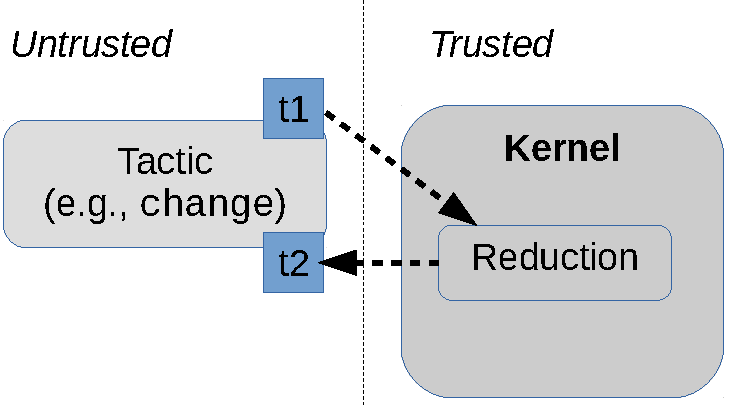
\includegraphics[width=0.48\textwidth]{rewriting/trust1}
    \label{subfig:change}} \hfill %\\
  \subfloat[Rewriting via proved rules]{%
    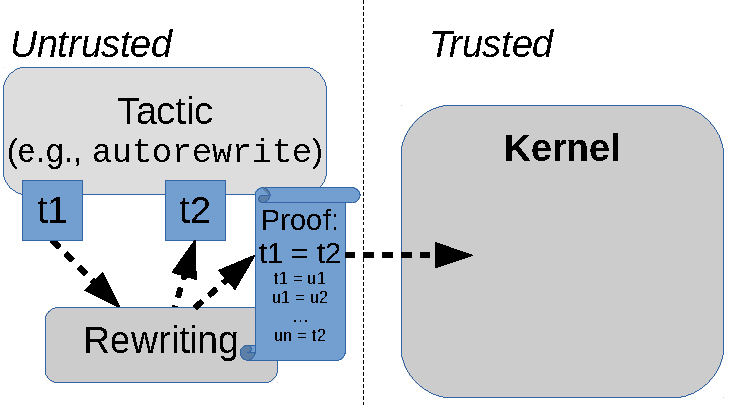
\includegraphics[width=0.48\textwidth]{rewriting/trust2}
    \label{subfig:autorewrite}} \\
  \subfloat[Approach of \textcite{Aehlig}]{%
    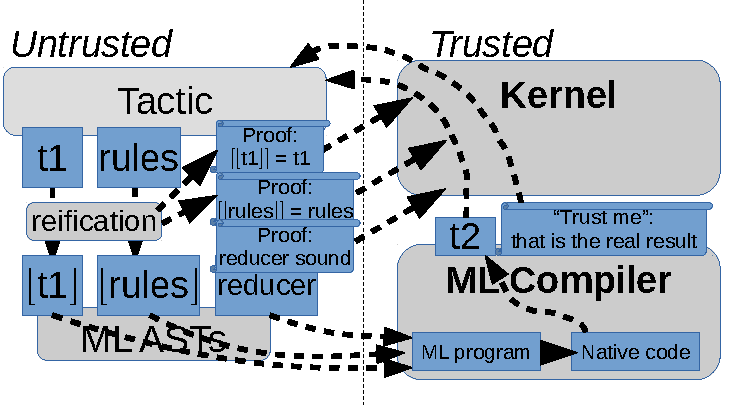
\includegraphics[width=0.48\textwidth]{rewriting/trust3}
    \label{subfig:aehlig}} \hfill %\\
  \subfloat[Our approach]{%
    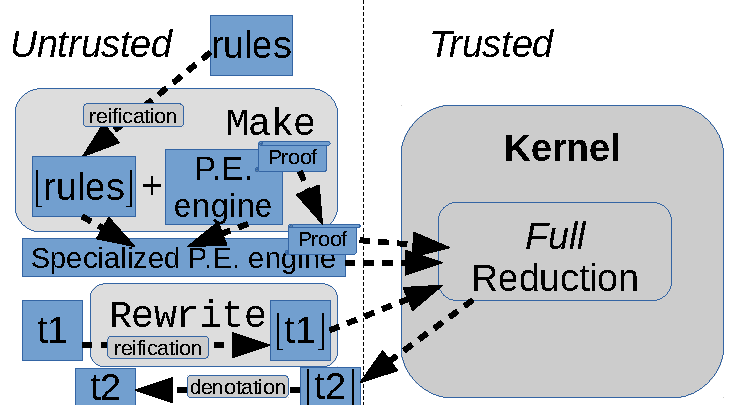
\includegraphics[width=0.48\textwidth]{rewriting/trust4}
    \label{subfig:perfect}}

  \caption{Different approaches to reduction and rewriting}
  \label{fig:trust}
\end{figure}

Now we summarize how \textcite{Aehlig} provide flexible and fast interleaving of standard $\lambda$-calculus reduction and use of proved equalities (the next section will go into more detail).
\autoref{subfig:aehlig} demonstrates a workflow based on \emph{a deep embedding of a core ML-like language}.
That is, within the logic of the proof assistant (Isabelle/HOL, in their case), a type of syntax trees for ML programs is defined, with an associated operational semantics.
The basic strategy is, for a particular set of rewrite rules and a particular term to simplify, to \emph{generate a (deeply embedded) ML program that, if it terminates, produces a syntax tree for the simplified term}.
Their tactic uses \emph{reification} to create ML versions of rule sets and terms.
They also wrote a reduction function in ML and proved it sound once and for all, against the ML operational semantics.
Combining that proof with proofs generated by reification, we conclude that an application of the reduction function to the reified rules and term is indeed an ML term that generates correct answers.
The tactic then ``throws the ML term over the wall,'' using a general code-generation framework for Isabelle/HOL~\cite{CodeGen}.
Trusted code compiles the ML code into the concrete syntax of a mainstream ML language, Standard ML in their case, and compiles it with an off-the-shelf compiler.
The output of that compiled program is then passed back over to the tactic, in terms of an axiomatic assertion that the ML semantics really yields that answer.

As \textcite{Aehlig} argue, their use of external compilation and evaluation of ML code adds no real complexity on top of that required by the proof assistant -- after all, the proof assistant itself must be compiled and executed somehow.
However, the perceived increase of trusted code base is not spurious:
it is one thing to trust that the toolchain and execution environment used by the proof assistant and the partial evaluator are well-behaved,
and another to rely on two descriptions of ML (one deeply embedded in the proof assistant and another implied by the compiler) to agree on every detail of the semantics.
Furthermore, there still is new trusted code to translate from the deeply embedded ML subset into the concrete syntax of the full-scale ML language.
% Aehlig et al. defined an ML language quite specialized to their use case, building in exactly the one algebraic datatype they need to represent NbE results, and it is unsatisfying to add such a specialized translator to the trusted base.
% However, we could imagine using a very general deep embedding of the proof assistant in itself, as with Template-Coq~\cite{TemplateCoq}.
% In that case, the expansion of the trusted code base would be even more worrying, to include an interpretation function from a complete syntactic embedding of the language within itself.
% Any inconsistency between the mechanized operational semantics (which would not be small, for a full-scale practical logic) and the actual implementation could break logical soundness.
The vast majority of proof-assistant developments today rely on no such embeddings with associated mechanized semantics, so need we really add one to a proof-checking kernel to support efficient partial evaluation?

Our answer, diagrammed in \autoref{subfig:perfect}, shows a different way.
We still reify terms and rules into a deeply embedded language.
However, \emph{the reduction engine is implemented directly in the logic}, rather than as a deeply embedded syntax tree of an ML program.
As a result, the kernel's own reduction engine is prepared to execute our reduction engine for us -- using an operation that would be included in a type-theoretic proof assistant in any case, with no special support for a language deep embedding.
We also stage the process for performance reasons.
First, the \mintinline{coq}{Make} command creates a rewriter out of a list of rewrite rules, by specializing a generic partial-evaluation engine, which has a generic proof that applies to any set of proved rewrite rules.
We perform partial evaluation on the specialized partial evaluator, using Coq's normal reduction mechanisms, under the theory that we can afford to pay performance costs at this stage because we only need to create new rewriters relatively infrequently.
Then individual rewritings involve reifying terms, asking the kernel to execute the specialized evaluator on them, and simplifying an application of an interpretation function to the result (this last step must be done using Coq's normal reduction, and it is the bottleneck for outputs with enormous numbers of nested binders as discussed in section \ref{sec:micro}).

We would like to emphasize that, while we prototyped our implementation in Coq in particular, the trade-off space that we navigate seems fundamental, so that it should be the case both that our approach can be adapted to other proof assistants and that this case study may inform proof-assistant design.
The general game here is to stock the trusted proof-checking kernel with as few primitive rules as we can get away with, while still providing enough flexibility and performance.
Every proof assistant we are aware of has a small functional language at its core, and we argue that is quite natural to include a primitive for efficient full reduction of programs.
Our empirical result is that such a primitive can form the basis for bootstrapping other kinds of efficient reduction, perhaps suggesting that a future Coq version could fruitfully shrink its kernel by eliminating other built-in reduction strategies.

\subsection{Our Approach in Nine Steps} \label{sec:nine-steps}

Here is a bit more detail on the steps that go into applying our Coq plugin, many of which we expand on in the following sections.
In order to build a precomputed rewriter with the \mintinline{coq}{Make} command, the following actions are performed:
\begin{enumerate}
\item
  The given lemma statements are scraped for which named functions and types the rewriter package will support.
\item
  Inductive types enumerating all available primitive types and functions are emitted.
\item
  Tactics generate all of the necessary definitions and prove all of the necessary lemmas for dealing with this particular set of inductive codes.
  Definitions include operations like Boolean equality on type codes and lemmas like ``all representable primitive types have decidable equality.''
\item
  The statements of rewrite rules are reified and soundness and syntactic-well-formedness lemmas are proven about each of them.
  Each instance of the former involves wrapping the user-provided proof with the right adapter to apply to the reified version.
\item
  The definitions needed to perform reification and rewriting and the lemmas needed to prove correctness are assembled into a single package that can be passed by name to the rewriting tactic.
\end{enumerate}

When we want to rewrite with a rewriter package in a goal, the following steps are performed:
\begin{enumerate}
\item
  We rearrange the goal into a single logical formula: all free-variable quantification in the proof context is replaced by changing the equality goal into an equality between two functions (taking the free variables as inputs).
  %\todo{Pedantic Note From Jason: it's not actually an equality between two functions, it's an \mintinline{coq}{equiv} between two functions where \mintinline{coq}{equiv} is a custom relation we define indexed over type codes that is equality up to function extensionality}
\item
  We reify the side of the goal we want to simplify, using the inductive codes in the specified package.  That side of the goal is then replaced with a call to a denotation function on the reified version.
\item
  We use a theorem stating that rewriting preserves denotations of well-formed terms to replace the denotation subterm with the denotation of the rewriter applied to the same reified term.
  We use Coq's built-in full reduction (\texttt{vm\_compute}) to reduce the application of the rewriter to the reified term.
\item
  Finally, we run \texttt{cbv} (a standard call-by-value reducer) to simplify away the invocation of the denotation function on the concrete syntax tree from rewriting.
  %\todo{Is it worth mentioning that we'd instead use \texttt{vm\_compute} if it supported whitelists (and also said whitelists were recorded in the casts)?}
\end{enumerate}


\section{The Structure of a Rewriter} \label{sec:structure}

We now simultaneously review the approach of \textcite{Aehlig} and introduce some notable differences in our own approach, noting similarities to the reflective rewriter of \textcite{rtac} where applicable.

First, let us describe the language of terms we support rewriting in.
Note that, while we support rewriting in full-scale Coq proofs, where the metalanguage is dependently typed, the object language of our rewriter is nearly simply typed, with limited support for calling polymorphic functions.
However, we still support identifiers whose definitions use dependent types, since our reducer does not need to look into definitions.
\begin{align*}
  e ::={}& \phantom{\mid} \texttt{App }e_1\texttt{ }e_2 \mid \texttt{Let }v \defeq e_1\texttt{ In }e_2 %\\
  %&
  \mid \texttt{Abs }(\lambda v.\,e) \mid \texttt{Var }v \mid \texttt{Ident }i
\end{align*}
The \texttt{Ident} case is for identifiers, which are described by an enumeration specific to a use of our library.
For example, the identifiers might be codes for $+$, $\cdot$, and literal constants.
We write $\llbracket e \rrbracket$ for a standard denotational semantics.

\subsection{Pattern-Matching Compilation and Evaluation} \label{sec:pattern-matching-compilation-and-evaluation}

\textcite{Aehlig} feed a specific set of user-provided rewrite rules to their engine by generating code for an ML function, which takes in deeply embedded term syntax (actually \emph{doubly} deeply embedded, within the syntax of the deeply embedded ML!) and uses ML pattern matching to decide which rule to apply at the top level.
Thus, they delegate efficient implementation of pattern matching to the underlying ML implementation.
As we instead build our rewriter in Coq's logic, we have no such option to defer to ML.
Indeed, Coq's logic only includes primitive pattern-matching constructs to match one constructor at a time.
%The frontend desugars nested pattern matching into trees of matches, but we do not have access to that desugaring within the language.
%It is arguably a good design decision to keep Coq working this way, since putting efficient nested pattern matching into the kernel would grow the trusted base substantially.

We could follow a naive strategy of repeatedly matching each subterm against a pattern for every rewrite rule, as in the rewriter of \textcite{rtac}, but in that case we do a lot of duplicate work when rewrite rules use overlapping function symbols.
Instead, we adopted the approach of \textcite{maranget2008compiling}, who describes compilation of pattern matches in OCaml to decision trees that eliminate needless repeated work (for example, decomposing an expression into $x + y + z$ only once even if two different rules match on that pattern).
We have not yet implemented any of the optimizations described therein for finding \emph{minimal} decision trees.

There are three steps to turn a set of rewrite rules into a functional program that takes in an expression and reduces according to the rules.
The first step is pattern-matching compilation: we must compile the left-hand sides of the rewrite rules to a decision tree that describes how and in what order to decompose the expression, as well as describing which rewrite rules to try at which steps of decomposition.
Because the decision tree is merely a decomposition hint, we require no proofs about it to ensure soundness of our rewriter.
The second step is decision-tree evaluation, during which we decompose the expression as per the decision tree, selecting which rewrite rules to attempt.
The only correctness lemma needed for this stage is that any result it returns is equivalent to picking some rewrite rule and rewriting with it.
The third and final step is to actually rewrite with the chosen rule.
Here the correctness condition is that we must not change the semantics of the expression.
Said another way, any rewrite-rule replacement expression must match the semantics of the rewrite-rule pattern.

While pattern matching begins with comparing one pattern against one expression, Maranget's approach works with intermediate goals that check multiple patterns against multiple expressions.
A decision tree describes how to match a vector (or list) of patterns against a vector of expressions.
It is built from these constructors:
\begin{itemize}
  \item \texttt{TryLeaf k onfailure}: Try the $k^\text{th}$ rewrite rule; if it fails, keep going with \texttt{onfailure}.
  \item \texttt{Failure}: Abort; nothing left to try.
  \item \texttt{Switch icases app\_case default}:
    With the first element of the vector, match on its kind; if it is an identifier matching something in \texttt{icases}, which is a list of pairs of identifiers and decision trees, remove the first element of the vector and run that decision tree; if it is an application and \texttt{app\_case} is not \texttt{None}, try the \texttt{app\_case} decision tree, replacing the first element of each vector with the two elements of the function and the argument it is applied to; otherwise, do not modify the vectors and use the \texttt{default} decision tree.
  \item \texttt{Swap i cont}: Swap the first element of the vector with the $i^\texttt{th}$ element (0-indexed) and keep going with \texttt{cont}.
\end{itemize}

Consider the encoding of two simple example rewrite rules, where we follow Coq's \Ltac{} language in prefacing pattern variables with question marks.
\begin{align*}
  ?n + 0 & \to n %\\
  &
  \texttt{fst}_{\mathbb{Z},\mathbb{Z}}(?x, ?y) & \to x
\end{align*}
We embed them in an AST type for patterns, which largely follows our ASTs for expressions.
\begin{verbatim}
0. App (App (Ident +) Wildcard) (Ident (Literal 0))
1. App (Ident fst) (App (App (Ident pair) Wildcard) Wildcard)
\end{verbatim}
The decision tree produced is \label{sec:compiled-pattern}
\[\resizebox{230px}{!}{\xymatrix@R-1pc{
  *++[o][F-]\txt{} \ar[d]_{\txt{App}} \\
  *++[o][F-]\txt{} \ar[r]^-{\txt{App}} \ar@/_1.5pc/[dr]_{\txt{\texttt{fst}}} & *++[o][F-]\txt{} \ar[r]^-{+} & *++[o][F-]\txt{Swap 0$\leftrightarrow$1} \ar[r] & *++[o][F-]\txt{} \ar[rr]^-{\txt{\texttt{Literal~0}}} && *++[o][F-]\txt{TryLeaf 0} \\
  & *++[o][F-]\txt{} \ar[r]_-{\txt{App}} & *++[o][F-]\txt{} \ar[r]_-{\txt{App}} & *++[o][F-]\txt{} \ar[rr]_-{\txt{\texttt{pair}}} && *++[o][F-]\txt{TryLeaf 1}
}}\]
\noindent where every non-swap node implicitly has a ``default'' case arrow to \texttt{Failure} and circles represent \texttt{Switch} nodes.

We implement, in Coq's logic, an evaluator for these trees against terms.
Note that we use Coq's normal partial evaluation to turn our general decision-tree evaluator into a specialized matcher to get reasonable efficiency.
Although this partial evaluation of our partial evaluator is subject to the same performance challenges we highlighted in the introduction, it only has to be done once for each set of rewrite rules, and we are targeting cases where the time of per-goal reduction dominates this time of meta-compilation.

For our running example of two rules, specializing gives us this match expression.
\begin{minted}[fontsize=\small]{coq}
match e with
| App f y => match f with
  | Ident fst => match y with
    | App (App (Ident pair) x) y => x | _ => e end
  | App (Ident +) x => match y with
    | Ident (Literal 0) => x | _ => e end | _ => e end | _ => e end.
\end{minted}

\subsection{Adding Higher-Order Features} \label{sec:thunk-eval-subst-term}

Fast rewriting at the top level of a term is the key ingredient for supporting customized algebraic simplification.
However, not only do we want to rewrite throughout the structure of a term, but we also want to integrate with simplification of higher-order terms, in a way where we can prove to Coq that our syntax-simplification function always terminates.
Normalization by evaluation (NbE)~\cite{NbE} is an elegant technique for adding the latter aspect, in a way where we avoid needing to implement our own $\lambda$-term reducer or prove it terminating.

To orient expectations: we would like to enable the following reduction
\begin{align*}
  (\lambda f\ x\ y.\, f\ x\ y)\ (+)\ z\ 0 & \leadsto z
\end{align*}
\noindent using the rewrite rule
\begin{align*}
  ?n + 0 & \to n
\end{align*}

\textcite{Aehlig} also use NbE, and we begin by reviewing its most classic variant, for performing full $\beta$-reduction in a simply typed term in a guaranteed-terminating way.
The simply typed $\lambda$-calculus syntax we use is:
\begin{align*}
  t & ::= t \to t ~|~ b
  & e & ::= \lambda v.\, e ~|~ e~e ~|~ v ~|~ c
\end{align*}
\noindent with $v$ for variables, $c$ for constants, and $b$ for base types.

We can now define normalization by evaluation.
First, we choose a ``semantic'' representation for each syntactic type, which serves as the result type of an intermediate interpreter.
\begin{align*}
  \text{NbE}_t(t_1 \to t_2) & \defeq \text{NbE}_t(t_1) \to \text{NbE}_t(t_2) \\
  \text{NbE}_t(b) & \defeq \texttt{expr}(b)
\end{align*}
Function types are handled as in a simple denotational semantics, while base types receive the perhaps-counterintuitive treatment that the result of ``executing'' one is a syntactic expression of the same type.
We write $\texttt{expr}(b)$ for the metalanguage type of object-language syntax trees of type $b$, relying on a type family $\texttt{expr}$.

\begin{figure}%[b]
\begin{align*}
  \text{reify}_t & : \text{NbE}_t(t) \to \text{expr}(t) \\
  \text{reify}_{t_1 \to t_2}(f) & \defeq \lambda v.\,\text{reify}_{t_2}(f(\text{reflect}_{t_1}(v))) \\
  \text{reify}_{b}(f) & \defeq f \\ \noalign{\vskip7pt}
  \text{reflect}_t & : \text{expr}(t) \to \text{NbE}_t(t) \\
  \text{reflect}_{t_1\to t_2}(e) & \defeq \lambda x.\,\text{reflect}_{t_2}(e(\text{reify}_{t_1}(x)) \\
  \text{reflect}_{b}(e) & \defeq e \\ \noalign{\vskip7pt}
  \text{reduce} & : \text{expr}(t) \to \text{NbE}_t(t) \\
  \text{reduce}(\lambda v. \; e) & \defeq \lambda x. \; \text{reduce}([x/v]e) \\
  \text{reduce}(e_1~e_2) & \defeq \left(\text{reduce}(e_1)\right)(\text{reduce}(e_2)) \\
  \text{reduce}(x) & \defeq x \\
  \text{reduce}(c) & \defeq \text{reflect}(c) \\ \noalign{\vskip7pt}
  \text{NbE} & : \text{expr}(t) \to \text{expr}(t) \\
  \text{NbE}(e) & \defeq \text{reify}(\text{reduce}(e))
\end{align*}
\caption{\label{fig:nbe}Implementation of normalization by evaluation}
\end{figure}

Now the core of NbE, shown in \autoref{fig:nbe}, is a pair of dual functions reify and reflect, for converting back and forth between syntax and semantics of the object language, defined by primitive recursion on type syntax.
We split out analysis of term syntax in a separate function reduce, defined by primitive recursion on term syntax, when usually this functionality would be mixed in with reflect.
The reason for this choice will become clear when we extend NbE to handle our full problem domain.

% These definitions apply some of the usual corner-cutting that we see in on-paper descriptions of $\lambda$-term transformations.
We write $v$ for object-language variables and $x$ for metalanguage (Coq) variables, and we overload $\lambda$ notation using the metavariable kind to signal whether we are building a host $\lambda$ or a $\lambda$ syntax tree for the embedded language.
The crucial first clause for reduce replaces object-language variable $v$ with fresh metalanguage variable $x$, and then we are somehow tracking that all free variables in an argument to reduce must have been replaced with metalanguage variables by the time we reach them.
We reveal in \autoref{sec:PHOAS} the encoding decisions that make all the above legitimate, but first let us see how to integrate use of the rewriting operation from the previous section.
To fuse NbE with rewriting, we only modify the constant case of \texttt{reduce}.
First, we bind our specialized decision-tree engine under the name rewrite-head.
Recall that this function only tries to apply rewrite rules at the top level of its input.

In the constant case, we still reflect the constant, but underneath the binders introduced by full $\eta$-expansion, we perform one instance of rewriting.
In other words, we change this one function-definition clause:
\begin{align*}
  \text{reflect}_{b}(e) & \defeq \text{rewrite-head}(e)
\end{align*}

It is important to note that a constant of function type will be $\eta$-expanded only once for each syntactic occurrence in the starting term, though the expanded function is effectively a thunk, waiting to perform rewriting again each time it is called.
From first principles, it is not clear why such a strategy terminates on all possible input terms, though we work up to convincing Coq of that fact.

The details so far are essentially the same as in the approach of \textcite{Aehlig}.
Recall that their rewriter was implemented in a deeply embedded ML, while ours is implemented in Coq's logic, which enforces termination of all functions.
Aehlig et al. did not prove termination, which indeed does not hold for their rewriter in general, which works with untyped terms, not to mention the possibility of rule-specific ML functions that diverge themselves.
In contrast, we need to convince Coq up-front that our interleaved $\lambda$-term normalization and algebraic simplification always terminate.
Additionally, we need to prove that our rewriter preserves denotations of terms, which can easily devolve into tedious binder bookkeeping, depending on encoding.

The next section introduces the techniques we use to avoid explicit termination proof or binder bookkeeping, in the context of a more general analysis of scaling challenges.


\section{Scaling Challenges} \label{sec:scaling}

\textcite{Aehlig} only evaluated their implementation against closed programs.
What happens when we try to apply the approach to partial-evaluation problems that should generate thousands of lines of low-level code?

\subsection{Variable Environments Will Be Large} \label{sec:PHOAS}
We should think carefully about representation of ASTs, since many primitive operations on variables will run in the course of a single partial evaluation.
For instance, \textcite{Aehlig} reported a significant performance improvement changing variable nodes from using strings to using de Bruijn indices~\cite{debruijn1972}.
However, de Bruijn indices and other first-order representations remain painful to work with.
We often need to fix up indices in a term being substituted in a new context.
Even looking up a variable in an environment tends to incur linear time overhead, thanks to traversal of a list.
Perhaps we can do better with some kind of balanced-tree data structure, but there is a fundamental performance gap versus the arrays that can be used in imperative implementations.
Unfortunately, it is difficult to integrate arrays soundly in a logic.
Also, even ignoring performance overheads, tedious binder bookkeeping complicates proofs.

Our strategy is to use a variable encoding that pushes all first-order bookkeeping off on Coq's kernel, which is itself performance-tuned with some crucial pieces of imperative code.
Parametric higher-order abstract syntax (PHOAS)~\cite{PhoasICFP08} is a dependently typed encoding of syntax where binders are managed by the enclosing type system.
It allows for relatively easy implementation and proof for NbE, so we adopted it for our framework.

Here is the actual inductive definition of term syntax for our object language, PHOAS-style.
The characteristic oddity is that the core syntax type \texttt{expr} is parameterized on a dependent type family for representing variables.
However, the final representation type \texttt{Expr} uses first-class polymorphism over choices of variable type, bootstrapping on the metalanguage's parametricity to ensure that a syntax tree is agnostic to variable type.
\begin{minted}[fontsize=\small]{coq}
  Inductive type := arrow (s d : type) | base (b : base_type).
  Infix "→" := arrow.
  Inductive expr (var : type -> Type) : type -> Type :=
  | Var {t} (v : var t) : expr var t
  | Abs {s d} (f : var s -> expr var d) : expr var (s → d)
  | App {s d} (f : expr var (s → d)) (x : expr var s) : expr var d
  | Const {t} (c : const t) : expr var t
  Definition Expr (t : type) : Type := forall var, expr var t.
\end{minted}

A good example of encoding adequacy is assigning a simple denotational semantics.
First, a simple recursive function assigns meanings to types.
\begin{minted}[fontsize=\small]{coq}
Fixpoint denoteT (t : type) : Type
  := match t with
     | arrow s d => denoteT s -> denoteT d
     | base b    => denote_base_type b
     end.
\end{minted}

Next we see the convenience of being able to \emph{use} an expression by choosing how it should represent variables.
Specifically, it is natural to choose \emph{the type-denotation function itself} as the variable representation.
Especially note how this choice makes rigorous the convention we followed in the prior section (e.g., in the suspicious function-abstraction clause of function reduce), where a recursive function enforces that values have always been substituted for variables early enough.
\begin{minted}[fontsize=\small]{coq}
Fixpoint denoteE {t} (e : expr denoteT t) : denoteT t
  := match e with
     | Var v     => v
     | Abs f     => λ x, denoteE (f x)
     | App f x   => (denoteE f) (denoteE x)
     | Ident c   => denoteI c
     end.
Definition DenoteE {t} (E : Expr t) : denoteT t
  := denoteE (E denoteT).
\end{minted}

It is now easy to follow the same script in making our rewriting-enabled NbE fully formal.
Note especially the first clause of \texttt{reduce}, where we avoid variable substitution precisely because we have chosen to represent variables with normalized semantic values.
The subtlety there is that base-type semantic values are themselves expression syntax trees, which depend on a nested choice of variable representation, which we retain as a parameter throughout these recursive functions.
The final definition $\lambda$-quantifies over that choice.
\begin{minted}[fontsize=\small]{coq}
Fixpoint nbeT var (t : type) : Type
  := match t with
     | arrow s d => nbeT var s -> nbeT var d
     | base b    => expr var b
     end.
Fixpoint reify {var t} : nbeT var t -> expr var t
  := match t with
     | arrow s d => λ f, Abs (λ x, reify (f (reflect (Var x))))
     | base b    => λ e, e
     end
with reflect {var t} : expr var t -> nbeT var t
  := match t with
     | arrow s d => λ e, λ x, reflect (App e (reify x))
     | base b    => rewrite_head
     end.
Fixpoint reduce {var t}
  (e : expr (nbeT var) t) : nbeT var t
  := match e with
     | Abs e     => λ x, reduce (e (Var x))
     | App e1 e2 => (reduce e1) (reduce e2)
     | Var x     => x
     | Ident c   => reflect (Ident c)
     end.
Definition Rewrite {t} (E : Expr t) : Expr t
  := λ var, reify (reduce (E (nbeT var t))).
\end{minted}

One subtlety hidden above in implicit arguments is in the final clause of \texttt{reduce}, where the two applications of the \texttt{Ident} constructor use different variable representations.
With all those details hashed out, we can prove a pleasingly simple correctness theorem, with a lemma for each main definition, with inductive structure mirroring recursive structure of the definition, also appealing to correctness of last section's pattern-compilation operations.
$$\forall t, E : \mintinline{coq}{Expr t}. \; \llbracket \mintinline{coq}{Rewrite}(E) \rrbracket = \llbracket E \rrbracket$$

Even before getting to the correctness theorem, we needed to convince Coq that the function terminates.
While for \textcite{Aehlig}, a termination proof would have been a whole separate enterprise, it turns out that PHOAS and NbE line up so well that Coq accepts the above code with no additional termination proof.
As a result, the Coq kernel is ready to run our \mintinline{coq}{Rewrite} procedure during checking.

To understand how we now apply the soundness theorem in a tactic, it is important to note how the Coq kernel builds in reduction strategies.
These strategies have, to an extent, been tuned to work well to show equivalence between a simple denotational-semantics application and the semantic value it produces.
In contrast, it is rather difficult to code up one reduction strategy that works well for all partial-evaluation tasks.
Therefore, we should restrict ourselves to (1) running full reduction in the style of functional-language interpreters and (2) running normal reduction on ``known-good'' goals like correctness of evaluation of a denotational semantics on a concrete input.

Operationally, then, we apply our tactic in a goal containing a term $e$ that we want to partially evaluate.
In standard proof-by-reflection style, we \emph{reify} $e$ into some $E$ where $\llbracket E \rrbracket = e$, replacing $e$ accordingly, asking Coq's kernel to validate the equivalence via standard reduction.
Now we use the \mintinline{coq}{Rewrite} correctness theorem to replace $\llbracket E \rrbracket$ with $\llbracket \mintinline{coq}{Rewrite}(E) \rrbracket$.
Next we may ask the Coq kernel to simplify $\mintinline{coq}{Rewrite}(E)$ by \emph{full reduction via compilation to native code}, since we carefully designed $\mintinline{coq}{Rewrite}(E)$ and its dependencies to produce closed syntax trees, so that reduction will not get stuck pattern-matching on free variables.
Finally, where $E'$ is the result of that reduction, we simplify $\llbracket E' \rrbracket$ with standard reduction, producing a normal-looking Coq term.

%% The payoffs from fully satisfying Coq's type checker are:
%% \begin{enumerate}
%% \item We know that this procedure always terminates, and Coq's kernel is therefore willing to run the procedure for us implicitly during proof checking.  In a sense, we have bootstrapped this reduction strategy into the conversion rule of the type theory.
%% \item In that setting, all bookkeeping about variable binding and environments is handled by the kernel, whose implementation in OCaml allows certain efficient implementation strategies not available to us in the logic.
%% \end{enumerate}

\subsection{Subterm Sharing is Crucial} \label{sec:under-lets}

For some large-scale partial-evaluation problems, it is important to represent output programs with sharing of common subterms.
Redundantly inlining shared subterms can lead to exponential increase in space requirements.
Consider the Fiat Cryptography~\cite{FiatCryptoSP19} example of generating a 64-bit implementation of field arithmetic for the P-256 elliptic curve.
The library has been converted manually to continuation-passing style, allowing proper generation of \mintinline{coq}{let} binders, whose variables are often mentioned multiple times.
We ran their code generator (actually just a subset of its functionality, but optimized by us a bit further, as explained in \autoref{sec:macro}) on the P-256 example and found it took about 15 seconds to finish.
Then we modified reduction to inline \mintinline{coq}{let} binders instead of preserving them, at which point the reduction job terminated with an out-of-memory error, on a machine with 64 GB of RAM.
(The successful run uses under 2 GB.)

We see a tension here between performance and niceness of library implementation.
The Fiat Cryptography authors found it necessary to CPS-convert their code to coax Coq into adequate reduction performance.
Then all of their correctness theorems were complicated by reasoning about continuations.
It feels like a slippery slope on the path to implementing a domain-specific compiler, rather than taking advantage of the pleasing simplicity of partial evaluation on natural functional programs.
Our reduction engine takes shared-subterm preservation seriously while applying to libraries in direct style.

Our approach is \mintinline{coq}{let}-lifting: we lift \mintinline{coq}{let}s to top level, so that applications of functions to \mintinline{coq}{let}s are available for rewriting.
For example, we can perform the rewriting
\begin{align*}
  \texttt{map}\ (\lambda x.\, y+x)\ (\letin[{z:=e}{[0;1;2;z;z+1]}]) \\
  \leadsto \; \letin[{z:=e}{[y;y+1;y+2;y+z;y+(z+1)]}]
\end{align*}
using the rules
\begin{align*}
  \texttt{map}\ {?f}\ [] & \to []
  &
  \texttt{map}\ {?f}\ ({?x} :: {?xs}) & \to f\ x :: \texttt{map}\ f\ xs
  & {?n} + 0 & \to n %\\
\end{align*}

Our approach is to define a telescope-style type family called \mintinline{coq}{UnderLets}:
\begin{minted}[fontsize=\small]{coq}
Inductive UnderLets {var} (T : Type) :=
| Base (v : T)
| UnderLet {A}(e : @expr var A)(f : var A -> UnderLets T).
\end{minted}
A value of type \mintinline{coq}{UnderLets T} is a series of \texttt{let} binders (where each expression \mintinline{coq}{e} may mention earlier-bound variables) ending in a value of type \mintinline{coq}{T}.
It is easy to build various ``smart constructors'' working with this type, for instance to construct a function application by lifting the \texttt{let}s of both function and argument to a common top level.

Such constructors are used to implement an NbE strategy that outputs \mintinline{coq}{UnderLets} telescopes.
Recall that the NbE type interpretation mapped base types to expression syntax trees.
We now parameterize that type interpretation by a Boolean declaring whether we want to introduce telescopes.

\begin{minted}[fontsize=\small]{coq}
Fixpoint nbeT' {var} (with_lets : bool) (t : type)
  := match t with
     | base t => if with_lets then @UnderLets var (@expr var t) else @expr var t
     | arrow s d => nbeT' false s -> nbeT' true d
     end.
Definition nbeT := nbeT' false.
Definition nbeT_with_lets := nbeT' true.
\end{minted}

%%  - Here are some examples:
%%    - `value Z := UnderLets (expr Z)`
%%    - `value (Z -> Z) := expr Z -> UnderLets (expr Z)`
%%    - `value (Z -> Z -> Z) := expr Z -> expr Z -> UnderLets (expr Z)`
%%    - `value ((Z -> Z) -> Z) := (expr Z -> UnderLets (expr Z)) -> UnderLets (expr Z)`

There are cases where naive preservation of \texttt{let} binders blocks later rewrites from triggering and leads to suboptimal performance, so we include some heuristics.
For instance, when the expression being bound is a constant, we always inline.
When the expression being bound is a series of list ``cons'' operations, we introduce a name for each individual list element, since such a list might be traversed multiple times in different ways.

\subsection{Rules Need Side Conditions} \label{sec:side-conditions}

Many useful algebraic simplifications require side conditions.
One simple case is supporting \emph{nonlinear} patterns, where a pattern variable appears multiple times.
We can encode nonlinearity on top of linear patterns via side conditions.
\begin{align*}
  {?n_1} + {?m} - {?n_2} & \to m\text{\ \ if\ \ }n_1 = n_2
\end{align*}

The trouble is how to support predictable solving of side conditions during partial evaluation, where we may be rewriting in open terms.
We decided to sidestep this problem by allowing side conditions only as executable Boolean functions, to be applied only to variables that are confirmed as \emph{compile-time constants}, unlike \textcite{rtac} who support general unification variables.
We added a variant of pattern variable that only matches constants.
Semantically, this variable style has no additional meaning, and in fact we implement it as a special identity function that should be called in the right places within Coq lemma statements.
Rather, use of this identity function triggers the right behavior in our tactic code that reifies lemma statements.
We introduce a notation where a prefixed apostrophe signals a call to the ``constants only'' function.

Our reification inspects the hypotheses of lemma statements, using type classes to find decidable realizations of the predicates that are used, synthesizing one Boolean expression of our deeply embedded term language, standing for a decision procedure for the hypotheses.
The \mintinline{coq}{Make} command fails if any such expression contains pattern variables not marked as constants.
Therefore, matching of rules can safely run side conditions, knowing that Coq's full-reduction engine can determine their truth efficiently.

\subsection{Side Conditions Need Abstract Interpretation} \label{sec:abs-int}

With our limitation that side conditions are decided by executable Boolean procedures, we cannot yet handle directly some of the rewrites needed for realistic partial evaluation.
For instance, Fiat Cryptography reduces high-level functional to low-level code that only uses integer types available on the target hardware.
The starting library code works with arbitrary-precision integers, while the generated low-level code should be careful to avoid unintended integer overflow.
As a result, the setup may be too naive for our running example rule ${?n} + 0 \to n$.
When we get to reducing fixed-precision-integer terms, we must be legalistic:
\begin{align*}
  \texttt{add\_with\_carry}_{64}({?n}, 0) & \to (0, n)\text{\ \ if\ \ }0 \le n < 2^{64}
\end{align*}

We developed a design pattern to handle this kind of rule.

First, we introduce a family of functions $\texttt{clip}_{l,u}$, each of which forces its integer argument to respect lower bound $l$ and upper bound $u$.
Partial evaluation is proved with respect to unknown realizations of these functions, only requiring that $\texttt{clip}_{l, u}(n) = n$ when $l \leq n < u$.
Now, before we begin partial evaluation, we can run a verified abstract interpreter to find conservative bounds for each program variable.
When bounds $l$ and $u$ are found for variable $x$, it is sound to replace $x$ with $\texttt{clip}_{l,u}(x)$.
Therefore, at the end of this phase, we assume all variable occurrences have been rewritten in this manner to record their proved bounds.

Second, we proceed with our example rule refactored:
\begin{align*}
  \texttt{add\_with\_carry}_{64}(\texttt{clip}_{'{?l},'{?u}}({?n}), 0) & \to (0, \texttt{clip}_{l,u}(n)) %\\
  %&
  \text{\ \ if\ \ }u < 2^{64}
\end{align*}
If the abstract interpreter did its job, then all lower and upper bounds are constants, and we can execute side conditions straightforwardly during pattern matching.

\subsection{Limitations and Preprocessing} \label{sec:implementation-and-usage}

%\todo{It's not clear to Jason what in this section belongs here, and what isn't interesting (yet?) to readers}
%\todo{I (Jason) have no idea what the story for this section should be}
%\todo{Insofar as text is actually kept in this section, make sure any duplication between here and the out-of-paper appendix is deliberate}
%\todo{If this section is moved or removed, be sure to restructure \autoref{sec:code-from-implementation-and-usage} accordingly}

We now note some details of the rewriting framework that were previously glossed over, which are useful for using the code or implementing something similar, but which do not add fundamental capabilities to the approach.
Although the rewriting framework does not support dependently typed constants, we can automatically preprocess uses of eliminators like \mintinline{coq}{nat_rect} and \mintinline{coq}{list_rect} into non-dependent versions.
The tactic that does this preprocessing is extensible via \Ltac{}'s reassignment feature.
Since pattern-matching compilation mixed with NbE requires knowing how many arguments a constant can be applied to, internally we must use a version of the recursion principle whose type arguments do not contain arrows; current preprocessing can handle recursion principles with either no arrows or one arrow in the motive.

Recall from \autoref{sec:explain-eval-rect} that \mintinline{coq}{eval_rect} is a definition provided by our framework for eagerly evaluating recursion associated with certain types.
It functions by triggering typeclass resolution for the lemmas reducing the recursion principle associated to the given type.
We provide instances for \texttt{nat}, \texttt{prod}, \texttt{list}, \texttt{option}, and \texttt{bool}.
Users may add more instances if they desire.

Recall again from \autoref{sec:explain-ident.eagerly} that we use \mintinline{coq}{ident.eagerly} to ask the reducer to simplify a case of primitive recursion by complete traversal of the designated argument's constructor tree.
Our current version only allows a limited, hard-coded set of eliminators with \mintinline{coq}{ident.eagerly} (\texttt{nat\_rect} on return types with either zero or one arrows, \texttt{list\_rect} on return types with either zero or one arrows, and \texttt{List.nth\_default}), but nothing in principle prevents automatic generation of the necessary code.

Note that \mintinline{coq}{Let_In} is the constant we use for writing \letin{} expressions that do not reduce under $\zeta$ (Coq's reduction rule for \mintinline{coq}{let}-inlining).
Throughout most of this paper, anywhere that \letin{} appears, we have actually used \mintinline{coq}{Let_In} in the code.
It would alternatively be possible to extend the reification preprocessor to automatically convert \letin{} to \mintinline{coq}{Let_In}, but this strategy may cause problems when converting the interpretation of the reified term with the pre-reified term, as Coq's conversion does not allow fine-tuning of when to inline or unfold \mintinline{coq}{let}s.

\section{Evaluation}\label{sec:evaluation}

% TODO: Presumably ``attached to this submission as an anonymized supplement'' will change for the final submission
Our implementation, attached to this submission as an anonymized supplement with a roadmap in \autoref{sec:CodeSupplement-more}, includes a mix of Coq code for the proved core of rewriting, tactic code for setting up proper use of that core, and OCaml plugin code for the manipulations beyond the current capabilities of the tactic language.
We report here on experiments to isolate performance benefits for rewriting under binders and reducing higher-order structure.

\subsection{Microbenchmarks} \label{sec:micro}

\def\NoBindersSubfloatNval{3}%
\def\NoBindersSubfloatXRow{\thisrowno{0}*(2^(\nval+1)-1)}%

We start with microbenchmarks focusing attention on particular aspects of reduction and rewriting, with \autoref{sec:additionalMicro} going into more detail.

\subsubsection{Rewriting Without Binders} \label{sec:micro:Plus0Tree}

Consider the code defined by the expression $\text{tree}_{n,m}(v)$ in \autoref{fig:micro:Plus0Tree:code}.
%\todo{make sure the figure spacing is okay}
%RSolve[{t[0]==m, t[n]==2*t[n-1] + m},t[n],n]
%t[n]=m(2^{n+1}-1)
We want to remove all of the${}+0$s.
There are $\Theta(m \cdot 2^n)$ such rewriting locations.
We can start from this expression directly, in which case reification alone takes as much time as Coq's \texttt{rewrite}.
\begin{wrapfigure}[7]{r}{0pt}
{\small $\begin{aligned}
\text{iter}_m(v) & = v + \underbrace{0 + 0 + \cdots + 0}_m \\
\text{tree}_{0,m}(v) &= \text{iter}_m(v + v) \\
\text{tree}_{n+1,m}(v) &= \text{iter}_m(\text{tree}_{n,m}(v) + \text{tree}_{n,m}(v))
\end{aligned}$}%
\caption{\label{fig:micro:Plus0Tree:code}Expressions computing initial code}
\end{wrapfigure}
As the reification method was not especially optimized, and there exist fast reification methods~\cite{ReificationITP18}, we instead start from a call to a recursive function that generates such an expression.


\begin{figure*}[b]
  \newsavebox{\NestedBindersSubfloat}%
  \sbox{\NestedBindersSubfloat}{%
    \adjustbox{valign=t}{\resizebox{0.4\textwidth}{!}{\beginTikzpictureStamped[only marks]{
      \einput{rewriting/perf-UnderLetsPlus0-cbv;rewrite-strat(bottomup).txt}
      \einput{rewriting/perf-UnderLetsPlus0-cbv;rewrite-strat(topdown).txt}
      \einput{rewriting/perf-UnderLetsPlus0-cbv;setoid-rewrite.txt}
      \einput{rewriting/perf-UnderLetsPlus0-Rewrite-for.txt}
      \einput{rewriting/perf-UnderLetsPlus0-rewriting.txt}
    }
      \pgfplotsset{every axis legend/.append style={
          at={(0.5,-0.2)},
          anchor=north}}
      \begin{axis}[xlabel=\# of let binders,ylabel=time (s),ymax=65]
        \addplot[mark=o,color=red] table{rewriting/perf-UnderLetsPlus0-cbv;rewrite-strat(bottomup).txt};
        \addplot[mark=triangle,color=red] table{rewriting/perf-UnderLetsPlus0-cbv;rewrite-strat(topdown).txt};
        \addplot[mark=square,color=red] table{rewriting/perf-UnderLetsPlus0-cbv;setoid-rewrite.txt};
        \addplot[mark=+,color=blue] table{rewriting/perf-UnderLetsPlus0-Rewrite-for.txt};
        \addplot[mark=x,color=ForestGreen] table{rewriting/perf-UnderLetsPlus0-rewriting.txt};
        \legend{rewrite\_strat bottomup,rewrite\_strat topdown,setoid\_rewrite,{Our approach including reification, cbv, etc.},Our approach (only rewriting)}
      \end{axis}
    \end{tikzpicture}}}}%
  \newsavebox{\BindersAndRecursiveFunctionsSubfloat}%
  \sbox{\BindersAndRecursiveFunctionsSubfloat}{%
    \adjustbox{valign=t}{\resizebox{0.4\textwidth}{!}{\beginTikzpictureStamped[only marks]{
        \einput{rewriting/perf-LiftLetsMap-rewrite-strat(bottomup,bottomup).txt}
        \einput{rewriting/perf-LiftLetsMap-rewrite-strat(topdown,bottomup).txt}
        \einput{rewriting/perf-LiftLetsMap-setoid-rewrite.txt}
        \einput{rewriting/perf-LiftLetsMap-Rewrite-for.txt}
        \einput{rewriting/perf-LiftLetsMap-rewriting.txt}
        \einput{rewriting/perf-LiftLetsMap-cps+vm-compute.txt}
    }
      \pgfplotsset{every axis legend/.append style={
          at={(0.5,-0.2)},
          anchor=north}}
      \begin{axis}[xlabel=$n\cdot m$,ylabel=time (s),scaled x ticks=false,ymax=27]
        \addplot[mark=o,color=red] table{rewriting/perf-LiftLetsMap-rewrite-strat(bottomup,bottomup).txt};
        \addplot[mark=triangle,color=red] table{rewriting/perf-LiftLetsMap-rewrite-strat(topdown,bottomup).txt};
        \addplot[mark=square,color=red] table{rewriting/perf-LiftLetsMap-setoid-rewrite.txt};
        \addplot[mark=+,color=blue] table{rewriting/perf-LiftLetsMap-Rewrite-for.txt};
        \addplot[mark=x,color=ForestGreen] table{rewriting/perf-LiftLetsMap-rewriting.txt};
        \addplot[mark=*,color=purple] table{rewriting/perf-LiftLetsMap-cps+vm-compute.txt};
        \legend{rewrite\_strat bottomup,rewrite\_strat topdown,repeat setoid\_rewrite,{Our approach including reification, cbv, etc.},Our approach (only rewriting),cps+vm\_compute}
      \end{axis}
    \end{tikzpicture}}}}%
  \newsavebox{\NoBindersSubfloat}%
  \sbox{\NoBindersSubfloat}{%
    \edef\nval{\NoBindersSubfloatNval}%
    \adjustbox{valign=t}{\resizebox{0.4\textwidth}{!}{\beginTikzpictureStamped[only marks]{
        \einput{rewriting/perf-Plus0Tree-only-n-\nval-cbv;rewrite-strat(bottomup).txt}
        \einput{rewriting/perf-Plus0Tree-only-n-\nval-cbv;setoid-rewrite.txt}
        \einput{rewriting/perf-Plus0Tree-only-n-\nval-cbv;rewrite-strat(topdown).txt}
        \einput{rewriting/perf-Plus0Tree-only-n-\nval-cbv;rewrite!.txt}
        \einput{rewriting/perf-Plus0Tree-only-n-\nval-Rewrite-for.txt}
        \einput{rewriting/perf-Plus0Tree-only-n-\nval-rewriting.txt}
        \nval
    }
      \pgfplotsset{every axis legend/.append style={
          at={(0.5,-0.2)},
          anchor=north}}
      % since n = 1, we have 2^n=twice as many rewrite locations as the value on the x axis, so we need to double things
      %,xticklabel={\pgfkeys{/pgf/fpu}\pgfmathparse{2^\nval*\tick}$\mathsf{\pgfmathprintnumber{\pgfmathresult}}$}
      \begin{axis}[xlabel=\# of rewrite locations,scaled x ticks=false,ylabel=time (s),ymax=7]% ymax=10]
        \addplot[mark=square,color=red] table[x expr={\NoBindersSubfloatXRow}]{rewriting/perf-Plus0Tree-only-n-\nval-cbv;rewrite-strat(bottomup).txt};
        \addplot[mark=*,color=red] table[x expr={\NoBindersSubfloatXRow}]{rewriting/perf-Plus0Tree-only-n-\nval-cbv;setoid-rewrite.txt};
        \addplot[mark=triangle,color=red] table[x expr={\NoBindersSubfloatXRow}]{rewriting/perf-Plus0Tree-only-n-\nval-cbv;rewrite-strat(topdown).txt};
        \addplot[mark=o,color=red] table[x expr={\NoBindersSubfloatXRow}]{rewriting/perf-Plus0Tree-only-n-\nval-cbv;rewrite!.txt};
        \addplot[mark=+,color=blue] table[x expr={\NoBindersSubfloatXRow}]{rewriting/perf-Plus0Tree-only-n-\nval-Rewrite-for.txt};
        \addplot[mark=x,color=ForestGreen] table[x expr={\NoBindersSubfloatXRow}]{rewriting/perf-Plus0Tree-only-n-\nval-rewriting.txt};
        \legend{rewrite\_strat bottomup,setoid\_rewrite,rewrite\_strat topdown,rewrite!,{Our approach including reification, cbv, etc.},Our approach (only rewriting)}
      \end{axis}
    \end{tikzpicture}}}}%
  \newsavebox{\FiatCryptoSubfloat}%
  \sbox{\FiatCryptoSubfloat}{%
    \adjustbox{valign=t}{\resizebox{0.4\textwidth}{!}{\beginTikzpictureStamped[only marks]{
      \einput{rewriting/perf-new-vm-over-old-vm.txt.md5}
      \einput{rewriting/perf-old-vm-over-old-vm.txt.md5}
      \einput{rewriting/perf-new-extraction-over-old-vm.txt.md5}
    }
      \pgfplotsset{every axis legend/.append style={
          at={(0.5,-0.2)},
          anchor=north}}
      \begin{axis}[xlabel=prime,ylabel=slowdown factor over old approach,xmode=log, ymode=log,log basis x={2}]
        \addplot[mark=+] table{rewriting/perf-new-vm-over-old-vm.txt};
        \addplot[mark=o] table{rewriting/perf-old-vm-over-old-vm.txt};
        \addplot[mark=*] table{rewriting/perf-new-extraction-over-old-vm.txt};
        \legend{Our approach w/ Coq's VM,Old approach (handwritten-CPS+VM),Our approach w/ extracted OCaml}
      \end{axis}
    \end{tikzpicture}}}}%
  \newcommand{\vphantomSubfloatOne}{\vphantom{\usebox{\NestedBindersSubfloat}}\vphantom{\usebox{\NoBindersSubfloat}}}%
  \newcommand{\vphantomSubfloatTwo}{\vphantom{\usebox{\BindersAndRecursiveFunctionsSubfloat}}\vphantom{\usebox{\FiatCryptoSubfloat}}}%
  \subfloat[No binders]{\usebox{\NoBindersSubfloat}\vphantomSubfloatOne\label{fig:timing-Plus0Tree}}%
  \quad
  \subfloat[Nested binders]{\usebox{\NestedBindersSubfloat}\vphantomSubfloatOne\label{fig:timing-UnderLetsPlus0}}%
  \quad
  \subfloat[Binders and recursive functions]{\usebox{\BindersAndRecursiveFunctionsSubfloat}\vphantomSubfloatTwo\label{fig:timing-LiftLetsMap}}%
  \quad
  \subfloat[Fiat Cryptography]{\usebox{\FiatCryptoSubfloat}\vphantomSubfloatTwo\label{fig:scaling}}

  \caption{Timing of different partial-evaluation implementations} \label{fig:multi-timing}
\end{figure*}

%RSolve[{t[0]==m, t[n]==2*t[n-1] + m},t[n],n]
%t[n]=m(2^{n+1}-1)
\autoref{fig:timing-Plus0Tree} shows the results for $n = \NoBindersSubfloatNval$ as we scale $m$.
The comparison points are Coq's \texttt{rewrite!}, \texttt{setoid\_rewrite}, and \texttt{rewrite\_strat}.
The first two perform one rewrite at a time, taking minimal advantage of commonalities across them and thus generating quite large, redundant proof terms.
The third makes top-down or bottom-up passes with combined generation of proof terms.
For our own approach, we list both the total time and the time taken for core execution of a verified rewrite engine, without counting reification (converting goals to ASTs) or its inverse (interpreting results back to normal-looking goals).

The comparison here is very favorable for our approach so long as $m > 2$.
The competing tactics spike upward toward timeouts at just around a thousand rewrite locations, while our engine is still under two seconds for examples with tens of thousands of rewrite locations.
When $m < 2$, Coq's \texttt{rewrite!} tactic does a little bit better than our engine, corresponding roughly to the overhead incurred by our term representation (which, for example, stores the types at every application node) when most of the term is in fact unchanged by rewriting.
See \autoref{sec:additionalPlots:Plus0Tree}\footnote{Like several forward references in this section, this one goes to an appendix included within the main submission page limit, to avoid interrupting the flow in presenting the most important results.} for more detailed plots.

\subsubsection{Rewriting Under Binders} \label{sec:micro:UnderLetsPlus0}

\begin{wrapfigure}[7]{r}{0pt}
{\small $\begin{aligned}
  & \letin[{v_1 := v_0 + v_0 + 0}{}] \\ \noalign{\vskip-7pt}
  & \vdots \\ \noalign{\vskip-3pt}
  & \letin[{v_n := v_{n-1} + v_{n-1} + 0}{}] \\
  & v_n + v_n + 0
\end{aligned}$}%
%  & \letin[{v_2 := v_1 + v_1 + 0}{}] \\
\caption{\label{fig:micro:UnderLetsPlus0:code}Initial code}
\end{wrapfigure}

Consider now the code in \autoref{fig:micro:UnderLetsPlus0:code}, which is a version of the code above where redundant expressions are shared via \mintinline{coq}{let} bindings.

\autoref{fig:timing-UnderLetsPlus0} shows the results.
The comparison here is again very favorable for our approach.
The competing tactics spike upward toward timeouts at just a few hundred generated binders, while our engine is only taking about 10 seconds for examples with 5,000 nested binders.

\subsubsection{Performance Bottlenecks of Proof-Producing Rewriting} \label{sec:micro:setoid-rewrite-bottlenecks-lite}

Although we have made our comparison against the built-in tactics \mintinline{coq}{setoid_rewrite} and \mintinline{coq}{rewrite_strat}, by analyzing the performance in detail, we can argue that these performance bottlenecks are likely to hold for any proof assistant designed like Coq.
Detailed debugging reveals five performance bottlenecks in the existing rewriting tactics, which we discuss in \autoref{sec:setoid-rewrite-bottlenecks}.\footnote{Also included within the submission page limit, though of interest mostly to proof-assistant-implementation experts.}

\subsubsection{Binders and Recursive Functions} \label{sec:micro:LiftLetsMap}

\begin{wrapfigure}[11]{r}{0pt}
{\small %\allowdisplaybreaks
$\begin{aligned}
  \text{map\_dbl}(\ell) & \defeq \begin{cases} [] & \text{if }\ell = [] \\
      \letin[{y := h + h}{}] & \text{if }\ell = h::t \\
      y :: \text{map\_dbl}(t) &
      \end{cases} \\
  \text{make}(n, m, v) & \defeq \begin{cases} [\underbrace{v, \ldots, v}_n] & \text{if }m = 0 \\
      \text{map\_dbl}(\text{make}(n, m-1, v)) & \text{if }m > 0
      \end{cases} \\
  \text{example}_{n, m} & \defeq \forall v,\ \text{make}(n, m, v) = []
\end{aligned}$}%
\caption{\label{fig:micro:LiftLetsMap:code}Initial code for binders and recursive functions}
\end{wrapfigure}

The next experiment uses the code in \autoref{fig:micro:LiftLetsMap:code}.
%Note that the ${}=[]$ at the end is just a dummy placeholder to allow us to check reduction and rewriting of this term.
Note that the \letin{} binding blocks further reduction of map\_dbl when we iterate it $m$ times in make, and so we need to take care to preserve sharing when reducing here.

\autoref{fig:timing-LiftLetsMap} compares performance between our approach, \texttt{repeat setoid\_rewrite}, and two variants of \texttt{rewrite\_strat}.
Additionally, we consider another option, which was adopted by Fiat Cryptography at a larger scale: rewrite our functions to improve reduction behavior.
Specifically, both functions are rewritten in continuation-passing style, which makes them harder to read and reason about but allows standard VM-based reduction to achieve good performance.
The figure shows that \texttt{rewrite\_strat} variants are essentially unusable for this example, with \texttt{setoid\_rewrite} performing only marginally better, while our approach applied to the original, more readable definitions loses ground steadily to VM-based reduction on CPS'd code.
On the largest terms ($n \cdot m > 20,000$), the gap is 6s vs.\ 0.1s of compilation time, which should often be acceptable in return for simplified coding and proofs, plus the ability to mix proved rewrite rules with built-in reductions.
Note that about 99\% of the difference between the full time of our method and just the rewriting is spent in the final \texttt{cbv} at the end, used to denote our output term from reified syntax.
We blame this performance on the unfortunate fact that reduction in Coq is quadratic in the number of nested binders present; see Coq bug \coqbug{11151}.
%traded for simplified coding and proofs, plus the ability to mix proved rewrite rules with built-in reductions.
See \autoref{sec:LiftLetsMap-more} for more on this microbenchmark.

\subsubsection{Full Reduction} \label{sec:micro:Eratosthenes}

\begin{wrapfigure}[18]{r}{0pt}
  \resizebox{0.4\textwidth}{!}{\beginTikzpictureStamped[only marks]{
      \einput{rewriting/perf-SieveOfEratosthenes-simpl.txt}
      \einput{rewriting/perf-SieveOfEratosthenes-cbn.txt}
      \einput{rewriting/perf-SieveOfEratosthenes-lazy.txt}
      \einput{rewriting/perf-SieveOfEratosthenes-Rewrite-for.txt}
      \einput{rewriting/perf-SieveOfEratosthenes-rewriting.txt}
      \einput{rewriting/perf-SieveOfEratosthenes-cbv.txt}
      \einput{rewriting/perf-SieveOfEratosthenes-vm-compute.txt}
      \einput{rewriting/perf-SieveOfEratosthenes-native(2)(real).txt}
  }
    \pgfplotsset{every axis legend/.append style={
        at={(0.5,-0.2)},
        anchor=north}}
    \begin{axis}[xlabel=upper bound,ylabel=time (s),ymax=65]
      \addplot[mark=square,color=red] table{rewriting/perf-SieveOfEratosthenes-simpl.txt};
      \addplot[mark=triangle,color=red] table{rewriting/perf-SieveOfEratosthenes-cbn.txt};
      \addplot[mark=square*,color=red] table{rewriting/perf-SieveOfEratosthenes-lazy.txt};
      \addplot[mark=+,color=blue] table{rewriting/perf-SieveOfEratosthenes-Rewrite-for.txt};
      \addplot[mark=x,color=ForestGreen] table{rewriting/perf-SieveOfEratosthenes-rewriting.txt};
      \addplot[mark=triangle*,color=orange] table{rewriting/perf-SieveOfEratosthenes-cbv.txt};
      \addplot[mark=*,color=purple] table{rewriting/perf-SieveOfEratosthenes-vm-compute.txt};
      \addplot[mark=-,color=red] table{rewriting/perf-SieveOfEratosthenes-native(2)(real).txt};
      \legend{simpl,cbn,lazy,{Our approach including reification, cbv, etc.},Our approach (only rewriting),cbv,vm\_compute,native\_compute}
    \end{axis}
  \end{tikzpicture}}
  \caption{\label{fig:timing-SieveOfEratosthenes}Full evaluation, Sieve of Eratosthenes}
\end{wrapfigure}

The final experiment involves full reduction in computing the Sieve of Eratosthenes, taking inspiration on benchmark choice from \textcite{Aehlig}.
We find in \autoref{fig:timing-SieveOfEratosthenes} that we are slower than \texttt{vm\_compute}, \mintinline{coq}{native_compute}, and \texttt{cbv}, but faster than \mintinline{coq}{lazy}, and of course much faster than \texttt{simpl} and \texttt{cbn}, which are quite slow.

\subsection{Macrobenchmark: Fiat Cryptography} \label{sec:macro}

Finally, we consider an experiment (described in more detail in \autoref{sec:additionalMacro}) replicating the generation of performance-competitive finite-field-arithmetic code for all popular elliptic curves by \textcite{FiatCryptoSP19}.
In all cases, we generate essentially the same code as they did, so we only measure performance of the code-generation process.
We stage partial evaluation with three different reduction engines (i.e., three \mintinline{coq}{Make} invocations), respectively applying 85, 56, and 44 rewrite rules (with only 2 rules shared across engines), taking total time of about 5 minutes to generate all three engines.
These engines support 95 distinct function symbols.

\autoref{fig:scaling} graphs running time of three different partial-evaluation methods for Fiat Cryptography, as the prime modulus of arithmetic scales up.
Times are normalized to the performance of the original method, which relied entirely on standard Coq reduction.
Actually, in the course of running this experiment, we found a way to improve the old approach for a fairer comparison.
It had relied on Coq's configurable \texttt{cbv} tactic to perform reduction with selected rules of the definitional equality, which the Fiat Cryptography developers had applied to blacklist identifiers that should be left for compile-time execution.
By instead hiding those identifiers behind opaque module-signature ascription, we were able to run Coq's more-optimized virtual-machine-based reducer.

As the figure shows, our approach running partial evaluation inside Coq's kernel begins with about a 10$\times$ performance disadvantage vs.\ the original method.
With log scale on both axes, we see that this disadvantage narrows to become nearly negligible for the largest primes, of around 500 bits.
(We used the same set of prime moduli as in the experiments run by \textcite{FiatCryptoSP19}, which were chosen based on searching the archives of an elliptic-curves mailing list for all prime numbers.)
It makes sense that execution inside Coq leaves our new approach at a disadvantage, as we are essentially running an interpreter (our normalizer) within an interpreter (Coq's kernel), while the old approach ran just the latter directly.
Also recall that the old approach required rewriting Fiat Cryptography's library of arithmetic functions in continuation-passing style, enduring this complexity in library correctness proofs, while our new approach applies to a direct-style library.
Finally, the old approach included a custom reflection-based arithmetic simplifier for term syntax, run after traditional reduction, whereas now we are able to apply a generic engine that combines both, without requiring more than proving traditional rewrite rules.

The figure also confirms clear performance advantage of running reduction in code extracted to OCaml, which is possible because our plugin produces verified code in Coq's functional language.
By the time we reach middle-of-the-pack prime size around 300 bits, the extracted version is running about 10$\times$ as quickly as the baseline.


\section{Related Work}\label{sec:related}

We have already discussed the work of \textcite{Aehlig}, which introduced the basic structure that our engine shares, but which required a substantially larger trusted code base, did not tackle certain challenges in scaling to large partial-evaluation problems, and did not report any performance experiments in partial evaluation.

We have also mentioned \Rtac{}~\cite{rtac}, which implements an experimental reflective version of \texttt{rewrite\_strat} supporting arbitrary setoid relations, unification variables, and arbitrary semi-decidable side conditions solvable by other reflective tactics, using de Bruijn indexing to manage binders.
We were unfortunately unable to get the rewriter to work with Coq 8.10 and were also not able to determine from the paper how to repurpose the rewriter to handle our benchmarks.

Our implementation builds on fast full reduction in Coq's kernel, via a virtual machine~\cite{vmcompute} or compilation to native code~\cite{nativecompute}.
Especially the latter is similar in adopting an NbE style for full reduction, simplifying even under $\lambda$s, on top of a more traditional implementation of OCaml that never executes preemptively under $\lambda$s.
Neither approach unifies support for rewriting with proved rules, and partial evaluation only applies in very limited cases, where functions that should not be evaluated at compile time must have properly opaque definitions that the evaluator will not consult.
Neither implementation involved a machine-checked proof suitable to bootstrap on top of reduction support in a kernel providing simpler reduction.

% A more limited form of code generation for cryptography was already widespread through libraries like OpenSSL, which specifically uses Perl scripts to generate assembly code.
% The Vale tool suite~\cite{Vale} formalizes these practices with a more principled language and associated verification tools.
% However, code generation done in this style is significantly simpler than what we treat here, amounting mostly to loop unrolling, macro substitution, and computation of compile-time constants.
% Also, Vale involves a significantly larger trusted code base than with our approach, with no reduction to some kernel proof checker, instead placing trust in language-specific tooling and an SMT solver.

A variety of forms of pragmatic partial evaluation have been demonstrated, with Lightweight Modular Staging~\cite{LMS} in Scala as one of the best-known current examples.
A kind of type-based overloading for staging annotations is used to smooth the rough edges in writing code that manipulates syntax trees.
The LMS-Verify system~\cite{LMSVerify} can be used for formal verification of generated code after-the-fact.
Typically LMS-Verify has been used with relatively shallow properties (though potentially applied to larger and more sophisticated code bases than we tackle), not scaling to the kinds of functional-correctness properties that concern us here, justifying investment in verified partial evaluators.

\section{Future Work}

There are a number of natural extensions to our engine.
For instance, we do not yet allow pattern variables marked as ``constants only'' to apply to container datatypes; we limit the mixing of higher-order and polymorphic types, as well as limiting use of first-class polymorphism; we do not support rewriting with equalities of non-fully-applied functions; we only support decidable predicates as rule side conditions, and the predicates may only mention pattern variables restricted to matching constants; we have hardcoded support for a small set of container types and their eliminators; we support rewriting with equality and no other relations (e.g., subset inclusion); and we require decidable equality for all types mentioned in rules.
It may be helpful to design an engine that lifts some or all of these limitations, building on the basic structure that we present here.

%%% Bibliography
%\clearpage
%\nocite{*}
%\bibliography{rewriting}
\clearpage

\begin{subappendices}
%\appendix

\section{Performance Bottlenecks of Proof-Producing Rewriting} \label{sec:setoid-rewrite-bottlenecks}

Although we have made our performance comparison against the built-in Coq tactics \mintinline{coq}{setoid_rewrite} and \mintinline{coq}{rewrite_strat}, by analyzing the performance in detail, we can argue that these performance bottlenecks are likely to hold for any proof assistant designed like Coq.
Detailed debugging reveals five performance bottlenecks in the existing rewriting tactics.
%(This section goes into detail that readers not interested in proof-assistant minutiae may want to skip, turning ahead to \autoref{sec:micro:LiftLetsMap}.)

\subsection{Bad performance scaling in sizes of existential-variable contexts}

We found that even when there are no occurrences fully matching the rule, \mintinline{coq}{setoid_rewrite} can still be \emph{cubic} in the number of binders (or, more accurately, quadratic in the number of binders with an additional multiplicative linear factor of the number of head-symbol matches).
Rewriting without any successful matches takes nearly as much time as \mintinline{coq}{setoid_rewrite} in this microbenchmark; by the time we are looking at goals with 400 binders, the difference is less than 5\%.

We posit that this overhead comes from \mintinline{coq}{setoid_rewrite} looking for head-symbol matches and then creating evars (existential variables) to instantiate the arguments of the lemmas for each head-symbol-match location; hence even if there are no matches of the rule as a whole, there may still be head-symbol matches.
Since Coq uses a locally nameless representation~\cite{LocallyNameless} for its terms, evar contexts are necessarily represented as \emph{named} contexts.
Representing a substitution between named contexts takes linear space, even when the substitution is trivial, and hence each evar incurs overhead linear in the number of binders above it.
Furthermore, fresh-name generation in Coq is quadratic in the size of the context, and since evar-context creation uses fresh-name generation, the additional multiplicative factor likely comes from fresh-name generation.
(Note, though, that this pattern suggests that the true performance is quartic rather than merely cubic.  However, doing a linear regression on a $\log$-$\log$ of the data suggests that the performance is genuinely cubic rather than quartic.)
%\todo{Can we cite an Coq issue that would de-anonymize us? 12524 (Andres says ``I would not cite, just claim coqdev acceptance if appropriate''}

Note that this overhead is inherent to the use of a locally nameless term representation.
To fix it, Coq would likely have to represent identity evar contexts using a compact representation, which is only naturally available for de Bruijn representations.
Any rewriting system that uses unification variables with a locally nameless (or named) context will incur at least quadratic overhead on this benchmark.

Note that \mintinline{coq}{rewrite_strat} uses exactly the same rewriting engine as \mintinline{coq}{setoid_rewrite}, just with a different strategy.
We found that \mintinline{coq}{setoid_rewrite} and \mintinline{coq}{rewrite_strat} have identical performance when there are no matches and generate identical proof terms when there are matches.
Hence we can conclude that the difference in performance between \mintinline{coq}{rewrite_strat} and \mintinline{coq}{setoid_rewrite} is entirely due to an increased number of failed rewrite attempts.

\subsection{Proof-term size}

Setting aside the performance bottleneck in constructing the matches in the first place, we can ask the question: how much cost is associated to the proof terms?
One way to ask this question in Coq is to see how long it takes to run \mintinline{coq}{Qed}.
While \mintinline{coq}{Qed}-time is asymptotically better, it is still quadratic in the number of binders.
This outcome is unsurprising, because the proof-term size is quadratic in the number of binders.
On this microbenchmark, we found that \mintinline{coq}{Qed}-time hits one second at about 250 binders, and using the best-fit quadratic line suggests that it would hit 10 seconds at about 800 binders and 100 seconds at about 2\,500 binders.
While this may be reasonable for the microbenchmarks, which only contain as many rewrite occurrences as there are binders, it would become unwieldy to try to build and typecheck such a proof with a rule for every primitive reduction step, which would be required if we want to avoid manually CPS-converting the code in Fiat Cryptography.

The quadratic factor in the proof term comes because we repeat subterms of the goal linearly in the number of rewrites.
For example, if we want to rewrite \mintinline{coq}{f (f x)} into \mintinline{coq}{g (g x)} by the equation \mintinline{coq}{∀ x, f x = g x}, then we will first rewrite \mintinline{coq}{f x} into \mintinline{coq}{g x}, and then rewrite \mintinline{coq}{f (g x)} into \mintinline{coq}{g (g x)}.
Note that \mintinline{coq}{g x} occurs three times (and will continue to occur in every subsequent step).

% We put this figure here so that the layout is better.
\begin{figure*}
\newcommand{\PlusZeroTreeMValSubfloat}[1]{%
  \def\mval{#1}%
  \subfloat[No binders ($m=\mval$)]{%
  \resizebox{0.4\textwidth}{!}{\beginTikzpictureStamped[only marks]{
    \einput{rewriting/perf-Plus0Tree-only-m-\mval-cbv;rewrite-strat(bottomup).txt}
    \einput{rewriting/perf-Plus0Tree-only-m-\mval-cbv;setoid-rewrite.txt}
    \einput{rewriting/perf-Plus0Tree-only-m-\mval-cbv;rewrite-strat(topdown).txt}
    \einput{rewriting/perf-Plus0Tree-only-m-\mval-cbv;rewrite!.txt}
    \einput{rewriting/perf-Plus0Tree-only-m-\mval-Rewrite-for.txt}
    \einput{rewriting/perf-Plus0Tree-only-m-\mval-rewriting.txt}
    \mval
  }
    \pgfplotsset{every axis legend/.append style={
        at={(0.5,-0.2)},
        anchor=north}}
    \begin{axis}[xlabel=$n$,ylabel=time (s),ymode=log,ymin=0.002,ymax=110]
      \addplot[mark=square,color=red] table{rewriting/perf-Plus0Tree-only-m-\mval-cbv;rewrite-strat(bottomup).txt};
      \addplot[mark=*,color=red] table{rewriting/perf-Plus0Tree-only-m-\mval-cbv;setoid-rewrite.txt};
      \addplot[mark=triangle,color=red] table{rewriting/perf-Plus0Tree-only-m-\mval-cbv;rewrite-strat(topdown).txt};
      \addplot[mark=o,color=red] table{rewriting/perf-Plus0Tree-only-m-\mval-cbv;rewrite!.txt};
      \addplot[mark=+,color=blue] table{rewriting/perf-Plus0Tree-only-m-\mval-Rewrite-for.txt};
      \addplot[mark=x,color=ForestGreen] table{rewriting/perf-Plus0Tree-only-m-\mval-rewriting.txt};
      \legend{rewrite\_strat bottomup,setoid\_rewrite,rewrite\_strat topdown,rewrite!,{Our approach including reification, cbv, etc.},Our approach (only rewriting)}
    \end{axis}
  \end{tikzpicture}}%
  \label{fig:timing-Plus0Tree-m=\mval}}%
}%
\PlusZeroTreeMValSubfloat{1}\qquad
\PlusZeroTreeMValSubfloat{2}\qquad
\PlusZeroTreeMValSubfloat{3}
  \caption{Timing of different partial-evaluation implementations for code with no binders for fixed $m$.  Note that we have a logarithmic time scale, because term size is proportional to $2^n$.} \label{fig:timing-Plus0Tree-fixed-m}
\end{figure*}

\subsection{Poor subterm sharing}

How easy is it to share subterms and create a linearly sized proof?
While it is relatively straightforward to share subterms using \mintinline{coq}{let} binders when the rewrite locations are not under any binders, it is not at all obvious how to share subterms when the terms occur under different binders.
Hence any rewriting algorithm that does not find a way to share subterms across different contexts will incur a quadratic factor in proof-building and proof-checking time, and we expect this factor will be significant enough to make applications to projects as large as Fiat Crypto infeasible.

\subsection{Overhead from the \mintinline{coq}{let} typing rule}

Suppose we had a proof-producing rewriting algorithm that shared subterms even under binders.
Would it be enough?
It turns out that even when the proof size is linear in the number of binders, the cost to typecheck it in Coq is still quadratic!
The reason is that when checking that \texttt{f : T} in a context \mintinline{coq}{x := v}, to check that \mintinline{coq}{let x := v in f} has type \texttt{T} (assuming that \mintinline{coq}{x} does not occur in \texttt{T}), Coq will substitute \mintinline{coq}{v} for \mintinline{coq}{x} in \texttt{T}.
So if a proof term has $n$ \mintinline{coq}{let} binders (e.g., used for sharing subterms), Coq will perform $n$ substitutions on the type of the proof term, even if none of the \mintinline{coq}{let}-binders are used.
If the number of \mintinline{coq}{let}-binders is linear in the size of the type, there is quadratic overhead in proof-checking time, even when the proof-term size is linear.

We performed a microbenchmark on a rewriting goal with no binders (because there is an obvious algorithm for sharing subterms in that case) and found that the proof-checking time reached about one second at about 2\,000 binders and reached 10 seconds at about 7\,000 binders.
While these results might seem good enough for Fiat Cryptography, we expect that there are hundreds of thousands of primitive reduction/rewriting steps even when there are only a few hundred binders in the output term, and we would need \mintinline{coq}{let}-binders for each of them.
Furthermore, we expect that getting such an algorithm correct would be quite tricky.

% We put this figure here so that the layout is better.
\begin{figure*}
\newcommand{\PlusZeroTreeNValSubfloat}[1]{%
  \def\nval{#1}%
  \subfloat[No binders ($n=\nval$)]{%
  \resizebox{0.4\textwidth}{!}{\beginTikzpictureStamped[only marks]{
      \einput{rewriting/perf-Plus0Tree-only-n-\nval-cbv;rewrite-strat(bottomup).txt}
      \einput{rewriting/perf-Plus0Tree-only-n-\nval-cbv;setoid-rewrite.txt}
      \einput{rewriting/perf-Plus0Tree-only-n-\nval-cbv;rewrite-strat(topdown).txt}
      \einput{rewriting/perf-Plus0Tree-only-n-\nval-cbv;rewrite!.txt}
      \einput{rewriting/perf-Plus0Tree-only-n-\nval-Rewrite-for.txt}
      \einput{rewriting/perf-Plus0Tree-only-n-\nval-rewriting.txt}
      \nval
  }
    \pgfplotsset{every axis legend/.append style={
        at={(0.5,-0.2)},
        anchor=north}}
    \begin{axis}[xlabel=$m$,ylabel=time (s),ymax=10]
      \addplot[mark=square,color=red] table{rewriting/perf-Plus0Tree-only-n-\nval-cbv;rewrite-strat(bottomup).txt};
      \addplot[mark=*,color=red] table{rewriting/perf-Plus0Tree-only-n-\nval-cbv;setoid-rewrite.txt};
      \addplot[mark=triangle,color=red] table{rewriting/perf-Plus0Tree-only-n-\nval-cbv;rewrite-strat(topdown).txt};
      \addplot[mark=o,color=red] table{rewriting/perf-Plus0Tree-only-n-\nval-cbv;rewrite!.txt};
      \addplot[mark=+,color=blue] table{rewriting/perf-Plus0Tree-only-n-\nval-Rewrite-for.txt};
      \addplot[mark=x,color=ForestGreen] table{rewriting/perf-Plus0Tree-only-n-\nval-rewriting.txt};
      \legend{rewrite\_strat bottomup,setoid\_rewrite,rewrite\_strat topdown,rewrite!,{Our approach including reification, cbv, etc.},Our approach (only rewriting)}
    \end{axis}
  \end{tikzpicture}}%
  \label{fig:timing-Plus0Tree-n=\nval}}%
}%
\PlusZeroTreeNValSubfloat{1}\qquad
\PlusZeroTreeNValSubfloat{2}\qquad
\PlusZeroTreeNValSubfloat{3}\qquad
%\PlusZeroTreeNValSubfloat{4}\qquad
%\PlusZeroTreeNValSubfloat{5}\qquad
%\PlusZeroTreeNValSubfloat{6}\qquad
%\PlusZeroTreeNValSubfloat{7}\qquad
%\PlusZeroTreeNValSubfloat{8}\qquad
\PlusZeroTreeNValSubfloat{9}
  \caption{Timing of different partial-evaluation implementations for code with no binders for fixed $n$ (1, 2, 3, and then we jump to 9)} \label{fig:timing-Plus0Tree-fixed-n}
\end{figure*}

% \begin{figure}
%   \begin{tikzpicture}[only marks]
%   \pgfplotsset{every axis legend/.append style={
%       at={(0.5,-0.2)},
%       anchor=north}}
%     \begin{axis}[xlabel=$\text{term size} = (m+1)\cdot 2^{n+1}-m$,ylabel=time (s)]
%       \addplot[mark=+,color=blue] table{rewriting/perf-Plus0Tree-Rewrite-for.txt};
%       \addplot[mark=x,color=ForestGreen] table{rewriting/perf-Plus0Tree-rewriting.txt};
%       \addplot[mark=o,color=red] table{rewriting/perf-Plus0Tree-cbv;rewrite!.txt};
%       \addplot[mark=*,color=red] table{rewriting/perf-Plus0Tree-cbv;setoid-rewrite.txt};
%       \addplot[mark=square,color=red] table{rewriting/perf-Plus0Tree-cbv;rewrite-strat(bottomup).txt};
%       \addplot[mark=triangle,color=red] table{rewriting/perf-Plus0Tree-cbv;rewrite-strat(topdown).txt};
%       \legend{Our approach including reification,Our approach (only rewriting),rewrite!,setoid\_rewrite,rewrite\_strat bottomup,rewrite\_strat topdown}
%     \end{axis}
%   \end{tikzpicture}
%   \caption{\label{fig:timing-Plus0Tree}Timing of different partial-evaluation implementations for code with no binders}
% \end{figure}

Fixing this quadratic bottleneck would, as far as we can tell, require deep changes in how Coq is implemented; it would either require reworking all of Coq to operate on some efficient representation of delayed substitutions paired with unsubstituted terms, or else it would require changing the typing rules of the type theory itself to remove this substitution from the typing rule for \mintinline{coq}{let}.
Note that there is a similar issue that crops up for function application and abstraction.

\subsection{Inherent advantages of reflection}

Finally, even if this quadratic bottleneck were fixed, \textcite{Aehlig} reported a $10\times$--$100\times$ speed-up over the \emph{simp} tactic in Isabelle, which performs all of the intermediate rewriting steps via the kernel API.
Their results suggest that even if all of the super-linear bottlenecks were fixed---no small undertaking---rewriting and partial evaluation via reflection might still be orders of magnitude faster than any proof-term-generating tactic.


\section{Additional Benchmarking Plots} \label{sec:additionalPlots}

\subsection{Rewriting Without Binders} \label{sec:additionalPlots:Plus0Tree}

The code in \autoref{fig:micro:Plus0Tree:code} in \autoref{sec:micro:Plus0Tree} is parameterized on both $n$, the height of the tree, and $m$, the number of rewriting occurrences per node.
The plot in \autoref{fig:timing-Plus0Tree} displays only the case of $n=\NoBindersSubfloatNval$.
The plots in \autoref{fig:timing-Plus0Tree-fixed-m} display how performance scales as a factor of $n$ for fixed $m$, and the plots in \autoref{fig:timing-Plus0Tree-fixed-n} display how performance scales as a factor of $m$ for fixed $n$.
Note the logarithmic scaling on the time axis in the plots in \autoref{fig:timing-Plus0Tree-fixed-m}, as term size is proportional to $m\cdot 2^n$.

We can see from these graphs and the ones in \autoref{fig:timing-Plus0Tree-fixed-n} that
(a) we incur constant overhead over most of the other methods, which dominates on small examples;
(b) when the term is quite large and there are few opportunities for rewriting relative to the term size (i.e., $m \le 2$), we are worse than \mintinline{coq}{rewrite !Z.add_0_r} but still better than the other methods; and
(c) when there are many opportunities for rewriting relative to the term size ($m > 2$), we thoroughly dominate the other methods.

\clearpage

\subsection{Additional Information on the Fiat Cryptography Benchmark} \label{sec:additionalPlots:FiatCrypto} \label{sec:additionalMacro}

\begin{figure*}[b]
  \newcommand{\MacroSubfloat}[3]{%
    \subfloat[Timing of different partial-evaluation implementations for Fiat Cryptography as prime modulus grows (only #2 #3)]{%
  \resizebox{0.45\textwidth}{!}{\beginTikzpictureStamped[only marks]{
      \einput{rewriting/perf-new-vm-times--only-#1-#3.txt}
      \einput{rewriting/perf-old-vm-times--only-#1-#3.txt}
      \einput{rewriting/perf-new-extraction-times--only-#1-#3.txt}
  }
    \pgfplotsset{every axis legend/.append style={
        at={(0.5,-0.2)},
        anchor=north}}
    \begin{axis}[xlabel=prime,ylabel=time (s),xmode=log, ymode=log,log basis x={2}]
      \addplot[mark=+] table{rewriting/perf-new-vm-times--only-#1-#3.txt};
      \addplot[mark=o] table{rewriting/perf-old-vm-times--only-#1-#3.txt};
      \addplot[mark=*] table{rewriting/perf-new-extraction-times--only-#1-#3.txt};
      \legend{Our approach w/ Coq's VM,Old approach (handwritten-CPS+VM),Our approach w/ extracted OCaml}
    \end{axis}
  \end{tikzpicture}}%
  \label{fig:timing--only-#1-#3}}%
  }%
  \MacroSubfloat{UnsaturatedSolinas}{unsaturated Solinas}{x32}\qquad
  \MacroSubfloat{UnsaturatedSolinas}{unsaturated Solinas}{x64}\\
  \MacroSubfloat{WordByWordMontgomery}{word-by-word Montgomery}{x32}\qquad
  \MacroSubfloat{WordByWordMontgomery}{word-by-word Montgomery}{x64}%
  \caption{\label{fig:timing-macro-various}Timing of different partial-evaluation implementations for Fiat Cryptography {vs.} prime modulus}
\end{figure*}

It may also be useful to see performance results with absolute times, rather than normalized execution ratios {vs.} the original Fiat Cryptography implementation.
Furthermore, the benchmarks fit into four quite different groupings: elements of the cross product of two algorithms (unsaturated Solinas and word-by-word Montgomery) and bitwidths of target architectures (32-bit or 64-bit).
Here we provide absolute-time graphs by grouping in \autoref{fig:timing-macro-various}.

\clearpage
%\supplement

\section{Additional Information on Microbenchmarks} \label{sec:additionalMicro}

We performed all benchmarks on a 3.5 GHz Intel Haswell running Linux and Coq 8.10.0.
We name the subsections here with the names that show up in the code supplement.

\subsection{UnderLetsPlus0} \label{sec:UnderLetsPlus0-more}

We provide more detail on the ``nested binders'' microbenchmark of \autoref{sec:micro:UnderLetsPlus0} displayed in \autoref{fig:timing-UnderLetsPlus0}.

Recall that we are removing all of the${}+0$s from
{\small \begin{align*}
  & \letin[{v_1 := v_0 + v_0 + 0}{}] \\
%  & \letin[{v_2 := v_1 + v_1 + 0}{}] \\
  & \vdots \\
  & \letin[{v_n := v_{n-1} + v_{n-1} + 0}{}] \\
  & v_n + v_n + 0
\end{align*}}%

The code used to define this microbenchmark is
\begin{minted}[fontsize=\small]{coq}
Definition make_lets_def (n:nat) (v acc : Z) :=
 @nat_rect (fun _ => Z * Z -> Z)
   (fun '(v, acc) => acc + acc + v)
   (fun _ rec '(v, acc) =>
     dlet acc := acc + acc + v in rec (v, acc))
   n
   (v, acc).
\end{minted}
We note some details of the rewriting framework that were glossed over in the main body of the paper, which are useful for using the code:
Although the rewriting framework does not support dependently typed constants, we can automatically preprocess uses of eliminators like \mintinline{coq}{nat_rect} and \mintinline{coq}{list_rect} into non-dependent versions.
The tactic that does this preprocessing is extensible via \Ltac{}'s reassignment feature.
Since pattern-matching compilation mixed with NbE requires knowing how many arguments a constant can be applied to, we must internally use a version of the recursion principle whose type arguments do not contain arrows; current preprocessing can handle recursion principles with either no arrows or one arrow in the motive.
Even though we will eventually plug in 0 for $v$, we jump through some extra hoops to ensure that our rewriter cannot cheat by rewriting away the ${}+0$ before reducing the recursion on $n$.

We can reduce this expression in three ways.

\subsubsection{Our Rewriter}
One lemma is required for rewriting with our rewriter:
\begin{minted}[fontsize=\small]{coq}
Lemma Z.add_0_r : forall z, z + 0 = z.
\end{minted}

Creating the rewriter takes about 12 seconds on the machine we used for running the performance experiments:
\begin{minted}[fontsize=\small]{coq}
Make myrew := Rewriter For (Z.add_0_r, eval_rect nat, eval_rect prod).
\end{minted}
Recall from \autoref{sec:explain-eval-rect} that \mintinline{coq}{eval_rect} is a definition provided by our framework for eagerly evaluating recursion associated with certain types.
It functions by triggering typeclass resolution for the lemmas reducing the recursion principle associated to the given type.
We provide instances for \texttt{nat}, \texttt{prod}, \texttt{list}, \texttt{option}, and \texttt{bool}.
Users may add more instances if they desire.

\subsubsection{\texorpdfstring{\texttt{setoid\_rewrite}}{setoid\_rewrite} and \texorpdfstring{\texttt{rewrite\_strat}}{rewrite\_strat}}
To give as many advantages as we can to the preexisting work on rewriting, we pre-reduce the recursion on \mintinline{coq}{nat}s using \texttt{cbv} before performing \texttt{setoid\_rewrite}.
(Note that \texttt{setoid\_rewrite} cannot itself perform reduction without generating large proof terms, and \texttt{rewrite\_strat} is not currently capable of sequencing reduction with rewriting internally due to bugs such as \coqbug{10923}.)
Rewriting itself is easy; we may use any of \texttt{repeat setoid\_rewrite Z.add\_0\_r}, \texttt{rewrite\_strat topdown Z.add\_0\_r}, or \texttt{rewrite\_strat bottomup Z.add\_0\_r}.

\subsection{Plus0Tree} \label{sec:Plus0Tree-more}

This is a version of \autoref{sec:UnderLetsPlus0-more} without any let binders, discussed in \autoref{sec:micro:Plus0Tree} but not displayed in \autoref{fig:multi-timing}.

We use two definitions for this microbenchmark:
\begin{minted}[fontsize=\small]{coq}
Definition iter (m : nat) (acc v : Z) :=
  @nat_rect (fun _ => Z -> Z)
    (fun acc => acc)
    (fun _ rec acc => rec (acc + v))
    m
    acc.
Definition make_tree (n m : nat) (v acc : Z) :=
 Eval cbv [iter] in
  @nat_rect (fun _ => Z * Z -> Z)
    (fun '(v, acc) => iter m (acc + acc) v)
    (fun _ rec '(v, acc) =>
      iter m (rec (v, acc) + rec (v, acc)) v)
    n
    (v, acc).
\end{minted}

\subsection{LiftLetsMap} \label{sec:LiftLetsMap-more}

We now discuss in more detail the ``binders and recursive functions'' example from \autoref{sec:micro:LiftLetsMap}.

The expression we want to get out at the end looks like:
\begin{align*}
    & \letin[{v_{1,1} := v + v}{}] \\
    & \vdots \\
    & \letin[{v_{1,n} := v + v}{}] \\
    & \letin[{v_{2,1} := v_{1,1} + v_{1,1}}{}] \\
    & \vdots \\
    & \letin[{v_{2,n} := v_{1,n} + v_{1,n}}{}] \\
    & \vdots \\
    & [v_{m,1}, \ldots, v_{m,n}]
\end{align*}

Recall that we make this example with the code
\begin{minted}[fontsize=\small]{coq}
Definition map_double (ls : list Z) :=
  list_rect _ [] (λ x xs rec, let y := x + x in y :: rec) ls.
Definition make (n : nat) (m : nat) (v : Z) :=
  nat_rect _ (List.repeat v n) (λ _ rec, map_double rec) m.
\end{minted}

We can perform this rewriting in four ways; see \autoref{fig:timing-LiftLetsMap}.

\subsubsection{Our Rewriter}
One lemma is required for rewriting with our rewriter:
\begin{minted}[fontsize=\small]{coq}
Lemma eval_repeat A x n
: @List.repeat A x ('n) = ident.eagerly nat_rect _ [] (λ k repeat_k, x :: repeat_k) ('n).
\end{minted}
Recall that the apostrophe marker (\verb|'|) is explained in \autoref{sec:explain-'}.
Recall again from \autoref{sec:explain-ident.eagerly} that we use \mintinline{coq}{ident.eagerly} to ask the reducer to simplify a case of primitive recursion by complete traversal of the designated argument's constructor tree.
Our current version only allows a limited, hard-coded set of eliminators with \mintinline{coq}{ident.eagerly} (\texttt{nat\_rect} on return types with either zero or one arrows, \texttt{list\_rect} on return types with either zero or one arrows, and \texttt{List.nth\_default}), but nothing in principle prevents automatic generation of the necessary code.
% Note that we use eliminators in the \mintinline{coq}{Thunked} namespace, which we provide in our library, to encode a version of the eliminator whose non-function cases are thunked rather than eagerly evaluated.
% That is, the type of, e.g., \mintinline{coq}{Thunked.nat_rect} is \mintinline{coq}{forall P, (unit -> P) -> (nat -> P -> P) -> nat -> P}.
% This is required in general for good performance with a call-by-value strategy, where you don't want to compute recursive cases that are then thrown away.
% Note that we don't really support any dependently typed constants; the use of \mintinline{coq}{nat_rect} in the first lemma is turned into a \mintinline{coq}{Thunked.nat_rect} automatically.
% Finally, we will note that our rewriter does not support matching on $\lambda$s on the left-hand-side, which is why the thunking cannot be done entirely internally on the left-hand-side.
% (It is performed during a preprocessing stage internally on the right-hand-side.)
% That is, the rewrite rule \emph{must} bind the thunked cases as part of the pattern.

We construct our rewriter with
\begin{minted}[fontsize=\small]{coq}
Make myrew := Rewriter For (eval_repeat, eval_rect list, eval_rect nat)
  (with extra idents (Z.add)).
\end{minted}
On the machine we used for running all our performance experiments, this command takes about 13 seconds to run.
Note that all identifiers which appear in any goal to be rewritten must either appear in the type of one of the rewrite rules or in the tuple passed to \texttt{with extra idents}.

Rewriting is relatively simple, now.
Simply invoke the tactic \mintinline{coq}{Rewrite_for myrew}.
We support rewriting on only the left-hand-side and on only the right-hand-side using either the tactic \mintinline{coq}{Rewrite_lhs_for myrew} or else the tactic \mintinline{coq}{Rewrite_rhs_for myrew}, respectively.

\subsubsection{\texorpdfstring{\texttt{rewrite\_strat}}{rewrite\_strat}}

To reduce adequately using \texttt{rewrite\_strat}, we need the following two lemmas:
\begin{minted}[fontsize=\small]{coq}
Lemma lift_let_list_rect T A P N C (v : A) fls
: @list_rect T P N C (Let_In v fls) = Let_In v (fun v => @list_rect T P N C (fls v)).
Lemma lift_let_cons T A x (v : A) f
: @cons T x (Let_In v f) = Let_In v (fun v => @cons T x (f v)).
\end{minted}

Note that \mintinline{coq}{Let_In} is the constant we use for writing \letin{} expressions that do not reduce under $\zeta$.
Throughout most of this paper, anywhere that \letin{} appears, we have actually used \mintinline{coq}{Let_In} in the code.
It would alternatively be possible to extend the reification preprocessor to automatically convert \letin{} to \mintinline{coq}{Let_In}, but this may cause problems when converting the interpretation of the reified term with the pre-reified term, as Coq's conversion does not allow fine-tuning of when to inline or unfold \mintinline{coq}{let}s.

To rewrite, we start with \mintinline{coq}{cbv [example make map_dbl]} to expose the underlying term to rewriting.
One would hope that one could just add these two hints to a database \mintinline{coq}{db} and then write \texttt{rewrite\_strat (repeat (eval cbn [list\_rect]; try bottomup hints db))}, but unfortunately this does not work due to a number of bugs in Coq: \coqbug{10934}, \coqbug{10923}, \coqbug{4175}, \coqbug{10955}, and the potential to hit \coqbug{10972}.
Instead, we must put the two lemmas in separate databases, and then write \texttt{repeat (cbn [list\_rect]; (rewrite\_strat (try repeat bottomup hints db1)); (rewrite\_strat (try repeat bottomup hints db2)))}.
Note that the rewriting with \mintinline{coq}{lift_let_cons} can be done either top-down or bottom-up, but \texttt{rewrite\_strat} breaks if the rewriting with \mintinline{coq}{lift_let_list_rect} is done top-down.

\subsubsection{CPS and the VM}
If we want to use Coq's built-in VM reduction without our rewriter, to achieve the prior state-of-the-art performance, we can do so on this example, because it only involves partial reduction and not equational rewriting.
However, we must (a) module-opacify the constants which are not to be unfolded, and (b) rewrite all of our code in CPS.

Then we are looking at
\begin{align*}
    \text{map\_dbl\_cps}(\ell,k) & \defeq \begin{cases} k([]) & \text{if }\ell = [] \\
        \letin[{y := h +_\text{ax} h}{}] & \text{if }\ell = h::t \\
        \text{map\_dbl\_cps}(t, \\
        \qquad(\lambda ys, k(y :: ys)))
    \end{cases} \\
    \text{make\_cps}(n, m, v, k) & \defeq \begin{cases} k([\underbrace{v, \ldots, v}_n]) & \text{if }m = 0 \\
        \text{make\_cps}(n, m-1, v, & \text{if }m > 0 \\
        \quad(\lambda \ell,\text{map\_dbl\_cps}(\ell, k))
    \end{cases} \\
    \text{example\_cps}_{n, m} & \defeq \forall v,\ \text{make\_cps}(n, m, v, \lambda x.\,x) = []
\end{align*}

Then we can just run \texttt{vm\_compute}.
Note that this strategy, while quite fast, results in a stack overflow when $n \cdot m$ is larger than approximately $2.5\cdot 10^4$.
This is unsurprising, as we are generating quite large terms.
Our framework can handle terms of this size but stack-overflows on only slightly larger terms.

\subsubsection{Takeaway}

From this example, we conclude that \texttt{rewrite\_strat} is unsuitable for computations involving large terms with many binders, especially in cases where reduction and rewriting need to be interwoven, and that the many bugs in \texttt{rewrite\_strat} result in confusing gymnastics required for success.
The prior state of the art---writing code in CPS---suitably tweaked by using module opacity to allow \texttt{vm\_compute}, remains the best performer here, though the cost of rewriting everything is CPS may be prohibitive.
Our method soundly beats \texttt{rewrite\_strat}.
We are additionally bottlenecked on \texttt{cbv}, which is used to unfold the goal post-rewriting and costs about a minute on the largest of terms; see Coq bug \coqbug{11151} for a discussion on what is wrong with Coq's reduction here.

\subsection{SieveOfEratosthenes} \label{sec:Eratosthenes}

We define the sieve using \mintinline{coq}{PositiveMap.t} and \mintinline{coq}{list Z}:
\begin{minted}[fontsize=\small]{coq}
Definition sieve' (fuel : nat) (max : Z) :=
 List.rev
  (fst
   (@nat_rect
    (λ _, list Z (* primes *) *
     PositiveSet.t (* composites *) *
     positive (* np (next_prime) *) ->
     list Z (* primes *) *
     PositiveSet.t (* composites *))
    (λ '(primes, composites, next_prime),
     (primes, composites))
    (λ _ rec '(primes, composites, np),
      rec
       (if (PositiveSet.mem np composites ||
            (Z.pos np >? max))%bool%Z
        then
         (primes, composites, Pos.succ np)
        else
         (Z.pos np :: primes,
          List.fold_right
           PositiveSet.add
           composites
           (List.map
            (λ n, Pos.mul (Pos.of_nat (S n)) np)
            (List.seq 0 (Z.to_nat(max/Z.pos np)))),
          Pos.succ np)))
    fuel
    (nil, PositiveSet.empty, 2%positive))).

Definition sieve (n : Z)
  := Eval cbv [sieve'] in sieve' (Z.to_nat n) n.
\end{minted}

We need four lemmas and an additional instance to create the rewriter:
\begin{minted}[fontsize=\small]{coq}
Lemma eval_fold_right A B f x ls :
@List.fold_right A B f x ls
= ident.eagerly list_rect _ _
    x
    (λ l ls fold_right_ls, f l fold_right_ls)
    ls.

Lemma eval_app A xs ys :
xs ++ ys
= ident.eagerly list_rect A _
    ys
    (λ x xs app_xs_ys, x :: app_xs_ys)
    xs.

Lemma eval_map A B f ls :
@List.map A B f ls
= ident.eagerly list_rect _ _
    []
    (λ l ls map_ls, f l :: map_ls)
    ls.

Lemma eval_rev A xs :
@List.rev A xs
= (@list_rect _ (fun _ => _))
    []
    (λ x xs rev_xs, rev_xs ++ [x])%list
    xs.

Scheme Equality for PositiveSet.tree.

Definition PositiveSet_t_beq
   : PositiveSet.t -> PositiveSet.t -> bool
  := tree_beq.

Global Instance PositiveSet_reflect_eqb
 : reflect_rel (@eq PositiveSet.t) PositiveSet_t_beq
 := reflect_of_brel
      internal_tree_dec_bl internal_tree_dec_lb.
\end{minted}

We then create the rewriter with
\begin{minted}[fontsize=\small]{coq}
Make myrew := Rewriter For
  (eval_rect nat, eval_rect prod, eval_fold_right,
   eval_map, do_again eval_rev, eval_rect bool,
   @fst_pair, eval_rect list, eval_app)
   (with extra idents (Z.eqb, orb, Z.gtb,
    PositiveSet.elements, @fst, @snd,
    PositiveSet.mem, Pos.succ, PositiveSet.add,
    List.fold_right, List.map, List.seq, Pos.mul,
    S, Pos.of_nat, Z.to_nat, Z.div, Z.pos, O,
    PositiveSet.empty))
  (with delta).
\end{minted}

To get \texttt{cbn} and \texttt{simpl} to unfold our term fully, we emit
\begin{minted}[fontsize=\small]{coq}
Global Arguments Pos.to_nat !_ / .
\end{minted}


\section{Experience vs.\ Lean and \texorpdfstring{\texttt{setoid\_rewrite}}{setoid\_rewrite}\label{sec:lean}}

Although all of our toy examples work with \texttt{setoid\_rewrite} or \texttt{rewrite\_strat} (until the terms get too big), even the smallest of examples in Fiat Cryptography fell over using these tactics.
When attempting to use \texttt{rewrite\_strat} for partial evaluation and rewriting on unsaturated Solinas with 1 limb on small primes (such as 29), we were able to get \texttt{rewrite\_strat} to finish after about 90 seconds.
The bugs in \texttt{rewrite\_strat} made finding the right magic invocation quite painful, nonetheless; the invocation we settled on involved \emph{sixteen} consecutive calls to \texttt{rewrite\_strat} with varying arguments and strategies.
Trying to synthesize code for two limbs on slightly larger primes (such as 113, which needs two limbs on a 64-bit machine) took about three hours.
The widely used primes tend to have around five to ten limbs; we leave extrapolating this slowdown to the reader.

We have attached this experiment using \verb|rewrite_strat| as \verb|fiat_crypto_via_rewrite_strat.v|, which is meant to be run in emacs/PG from inside the \verb|fiat-crypto| directory, or in \verb|coqc| by setting \verb|COQPATH| to the value emitted by \texttt{make printenv} in \verb|fiat-crypto| and then invoking the command \texttt{coqc -q -R /path/to/fiat-crypto/src Crypto /path/to/fiat\_crypto\_via\_rewrite\_strat.v}.
To test with the two-limb prime 113, change \verb|of_string "2^5-3" 8| in the definition of \verb|p| to \verb|of_string "2^7-15" 64|.

We also tried Lean, in the hopes that rewriting in Lean, specifically optimized for performance, would be up to the challenge.
Although Lean performed about 30\% better than Coq on the 1-limb example, taking a bit under a minute, it did not complete on the two-limb example even after four hours (after which we stopped trying), and a five-limb example was still going after 40 hours.

We have attached our experiments with running \texttt{rewrite} in Lean on the Fiat Cryptography code as a supplement as well.
We used Lean version 3.4.2, commit cbd2b6686ddb, Release.
Run \texttt{make} in \texttt{fiat-crypto-lean} to run the one-limb example;
change \texttt{open ex} to \texttt{open ex2} to try the two-limb example, or to \texttt{open ex5} to try the five-limb example.

\section{Reading the Code Supplement} \label{sec:CodeSupplement-more}

% allow breaks after slashes, for long paths
\catcode`\/=\active
\def/{\slash}%

We have attached both the code for implementing the rewriter, as well as a copy of Fiat Cryptography adapted to use the rewriting framework.
Both code supplements build with Coq 8.9 and Coq 8.10, and they require that whichever OCaml was used to build Coq be installed on the system to permit building plugins.
(If Coq was installed via opam, then the correct version of OCaml will automatically be available.)
Both code bases can be built by running \texttt{make} in the top-level directory.

The performance data for both repositories are included at the top level as \texttt{.txt} and \texttt{.csv} files.

The performance data for the microbenchmarks can be rebuilt using \texttt{make perf-SuperFast perf-Fast perf-Medium} followed by \texttt{make perf-csv} to get the \texttt{.txt} and \texttt{.csv} files.
The microbenchmarks should run in about 24 hours when run with \texttt{-j5} on a 3.5 GHz machine.
There also exist targets \texttt{perf-Slow} and \texttt{perf-VerySlow}, but these take significantly longer.

The performance data for the macrobenchmark can be rebuilt from the Fiat Cryptography copy included by running \texttt{make perf -k}.
We ran this with \texttt{PERF\_MAX\_TIME=3600} to allow each benchmark to run for up to an hour; the default is 10 minutes per benchmark.
Expect the benchmarks to take over a week of time with an hour timeout and five cores.
Some tests are expected to fail, making \texttt{-k} a necessary flag.
Again, the \texttt{perf-csv} target will aggregate the logs and turn them into \texttt{.txt} and \texttt{.csv} files.

The entry point for the rewriter is the Coq source file \texttt{rewriter/src/Rewriter/Util/plugins/RewriterBuild.v}.

The rewrite rules used in Fiat Cryptography are defined in \texttt{fiat-crypto/src/Rewriter/Rules.v} and proven in \texttt{fiat-crypto/src/Rewriter/RulesProofs.v}.
Note that the Fiat Cryptography copy uses \verb|COQPATH| for dependency management, and \verb|.dir-locals.el| to set \verb|COQPATH| in emacs/PG; you must accept the setting when opening a file in the directory for interactive compilation to work.
Thus interactive editing either requires ProofGeneral or manual setting of \verb|COQPATH|.
The correct value of \verb|COQPATH| can be found by running \verb|make printenv|.

We will now go through this paper and describe where to find each reference in the code base.

\newcommand{\autocommanameref}[1]{\autoref{#1}, \nameref{#1}}

\subsection{Code from \autocommanameref{sec:intro}}

\subsubsection{Code from \autocommanameref{sec:motivating-example}}

The \texttt{prefixSums} example appears in the Coq source file \texttt{rewriter/src/Rewriter/Rewriter/Examples/PrefixSums.v}.
Note that we use \texttt{dlet} rather than \mintinline{coq}{let} in binding \texttt{acc'} so that we can preserve the \mintinline{coq}{let} binder even under $\iota$ reduction, which much of Coq's infrastructure performs eagerly.
Because we attempt to isolate the dependency on the axiom of functional extensionality as much as possible, we also in practice require \texttt{Proper} instances for each higher-order identifier saying that each constant respects function extensionality.
We hope to remove the dependency on function extensionality altogether in the future.
Although we glossed over this detail in the body of this paper, we also prove
\begin{minted}[fontsize=\small]{coq}
Global Instance: forall A B,
 Proper ((eq ==> eq ==> eq) ==> eq ==> eq ==> eq)
        (@fold_left A B).
\end{minted}

The \mintinline{coq}{Make} command is exposed in \texttt{rewriter/src/Rewriter/Util/plugins/RewriterBuild.v} and defined in \texttt{rewriter/src/Rewriter/Util/plugins/rewriter\_build\_plugin.mlg}.
Note that one must run \texttt{make} to create this latter file; it is copied over from a version-specific file at the beginning of the build.

\label{sec:code:eval-rect}%
\label{sec:code:ident.eagerly}%
The \verb|do_again|, \verb|eval_rect|, and \verb|ident.eagerly| constants are defined at the bottom of module \verb|RewriteRuleNotations| in \texttt{rewriter/src/Rewriter/Language/Pre.v}.

\subsubsection{Code from \autocommanameref{sec:trusted-code-base-size}}

There is no code mentioned in this section.

\subsubsection{Code from \autocommanameref{sec:our-solution}}

We claimed that our solution meets five criteria.
We briefly justify each criterion with a sentence or a pointer to code:
\begin{itemize}
  \item
    We claimed that we \textbf{did not grow the trusted base} (excepting the axiom of functional extensionality).
    In any example file (of which a couple can be found in \texttt{rewriter/src/Rewriter/Rewriter/Examples/}), the \mintinline{coq}{Make} command creates a rewriter package.
    Running \texttt{Print Assumptions} on this new constant (often named \texttt{rewriter} or \texttt{myrew}) should demonstrate a lack of axioms other than functional extensionality.
    \texttt{Print Assumptions} may also be run on the proof that results from using the rewriter.
  \item
    We claimed \textbf{fast} partial evaluation with reasonable memory use; we assume that the performance graphs stand on their own to support this claim.
    Note that memory usage can be observed by making the benchmarks while passing \texttt{TIMED=1} to \texttt{make}.
  \item
    We claimed to allow reduction that \textbf{mixes} \emph{rules of the definitional equality} with \emph{equalities proven explicitly as theorems}; the ``rules of the definitional equality'' are, for example, $\beta$ reduction, and we assert that it should be self-evident that our rewriter supports this.
  \item
    We claimed common-subterm \textbf{sharing preservation}.
    This is implemented by supporting the use of the \texttt{dlet} notation which is defined in \texttt{rewriter/src/Rewriter/Util/LetIn.v} via the \texttt{Let\_In} constant.
    We will come back to the infrastructure that supports this.
  \item
    We claimed \textbf{extraction of standalone partial evaluators}.
    The extraction is performed in the files \texttt{perf\_unsaturated\_solinas.v} and \texttt{perf\_word\_by\_word\_montgomery.v}, and the files \texttt{saturated\_solinas.v}, \texttt{unsaturated\_solinas.v}, and \texttt{word\_by\_word\_montgomery.v}, all in the directory \texttt{fiat-crypto/src/ExtractionOCaml/}.
    The OCaml code can be extracted and built using the target \texttt{make standalone-ocaml} (or \texttt{make perf-standalone} for the \texttt{perf\_} binaries).
    There may be some issues with building these binaries on Windows as some versions of \texttt{ocamlopt} on Windows seem not to support outputting binaries without the \texttt{.exe} extension.
\end{itemize}

The P-384 curve is mentioned.
This is the curve with modulus $2^{384} - 2^{128} - 2^{96} + 2^{32} - 1$; its benchmarks can be found in files matching the glob \texttt{fiat-crypto/src/Rewriter/PerfTesting/Specific/generated/p2384m2128m296p232m1\_\_*\_\_word\_by\_word\_montgomery\_*}.
The output \texttt{.log} files are included in the tarball; the \texttt{.v} and \texttt{.sh} files are automatically generated in the course of running \texttt{make perf -k}.

We mention integration with abstract interpretation; the abstract-interpretation pass is implemented in \texttt{fiat-crypto/src/AbstractInterpretation/}.

\subsection{Code from \autocommanameref{sec:trust}}

The individual rewritings mentioned are implemented via the \texttt{Rewrite\_*} tactics exported at the top of \texttt{rewriter/src/Rewriter/Util/plugins/RewriterBuild.v}.
These tactics bottom out in tactics defined at the bottom of \texttt{rewriter/src/Rewriter/Rewriter/AllTactics.v}.

\subsubsection{Code from \autocommanameref{sec:nine-steps}} \label{sec:code:nine-steps}

We match the nine steps with functions from the source code:
\begin{enumerate}
  \item
    The given lemma statements are scraped for which named functions and types the rewriter package will support.
    This is performed by \texttt{rewriter\_scrape\_data} in the file \texttt{rewriter/src/Rewriter/Util/plugins/rewriter\_build.ml} which invokes the \Ltac{} tactic named \texttt{make\_scrape\_data} in a submodule in the source file \texttt{rewriter/src/Rewriter/Language/IdentifiersBasicGenerate.v} on a goal headed by the constant we provide under the name \texttt{Pre.ScrapedData.t\_with\_args} in \texttt{rewriter/src/Rewriter/Language/PreCommon.v}.
  \item
    Inductive types enumerating all available primitive types and functions are emitted.
    This step is performed by \texttt{rewriter\_emit\_inductives} in file \texttt{rewriter/src/Rewriter/Util/plugins/rewriter\_build.ml} invoking tactics, like \texttt{make\_base\_elim} in \texttt{rewriter/src/Rewriter/Language/IdentifiersBasicGenerate.v}, on goals headed by constants from \texttt{rewriter/src/Rewriter/Language/IdentifiersBasicLibrary.v}, including the constant \texttt{base\_elim\_with\_args} for example, to turn scraped data into eliminators for the inductives.
    The actual emitting of inductives is performed by code in the file \texttt{rewriter/src/Rewriter/Util/plugins/inductive\_from\_elim.ml}.
  \item
    Tactics generate all of the necessary definitions and prove all of the necessary lemmas for dealing with this particular set of inductive codes.
    This step is performed by the tactic \texttt{make\_rewriter\_of\_scraped\_and\_ind} in the source file \texttt{rewriter/src/Rewriter/Util/plugins/rewriter\_build.ml} which invokes the tactic \texttt{make\_rewriter\_all} defined in the file \texttt{rewriter/src/Rewriter/Rewriter/AllTactics.v} on a goal headed by the provided constant \texttt{VerifiedRewriter\_with\_ind\_args} defined in \texttt{rewriter/src/Rewriter/Rewriter/ProofsCommon.v}.
    The definitions emitted can be found by looking at the tactic \texttt{Build\_Rewriter} in \texttt{rewriter/src/Rewriter/Rewriter/AllTactics.v}, the \Ltac{} tactics \texttt{build\_package} in \texttt{rewriter/src/Rewriter/Language/IdentifiersBasicGenerate.v} and also in \texttt{rewriter/src/Rewriter/Language/IdentifiersGenerate.v} (there is a different tactic named \texttt{build\_package} in each of these files), and \texttt{prove\_package\_proofs\_via} which can be found in \texttt{rewriter/src/Rewriter/Language/IdentifiersGenerateProofs.v}.
  \item
    The statements of rewrite rules are reified and soundness and syntactic-well-formedness lemmas are proven about each of them.
    This is done as part of the previous step, when the tactic \texttt{make\_rewriter\_all} transitively calls \texttt{Build\_Rewriter} from \texttt{rewriter/src/Rewriter/Rewriter/AllTactics.v}.
    Reification is handled by the tactic \texttt{Build\_RewriterT} in \texttt{rewriter/src/Rewriter/Rewriter/Reify.v}, while soundness and the syntactic-well-formedness proofs are handled by the tactics \texttt{prove\_interp\_good} and \texttt{prove\_good} respectively, both in the source file \texttt{rewriter/src/Rewriter/Rewriter/ProofsCommonTactics.v}.
  \item
    The definitions needed to perform reification and rewriting and the lemmas needed to prove correctness are assembled into a single package that can be passed by name to the rewriting tactic.
    This step is also performed by \texttt{make\_rewriter\_of\_scraped\_and\_ind} in the source file \texttt{rewriter/src/Rewriter/Util/plugins/rewriter\_build.ml}.
\end{enumerate}

When we want to rewrite with a rewriter package in a goal, the following steps are performed, with code in the following places:
\begin{enumerate}
  \item
    We rearrange the goal into a closed logical formula: all free-variable quantification in the proof context is replaced by changing the equality goal into an equality between two functions (taking the free variables as inputs).
    Note that it is not actually an equality between two functions but rather an \texttt{equiv} between two functions, where \texttt{equiv} is a custom relation we define indexed over type codes that is equality up to function extensionality.
    This step is performed by the tactic \texttt{generalize\_hyps\_for\_rewriting} in \texttt{rewriter/src/Rewriter/Rewriter/AllTactics.v}.
  \item
    We reify the side of the goal we want to simplify, using the inductive codes in the specified package.  That side of the goal is then replaced with a call to a denotation function on the reified version.
    This step is performed by the tactic \texttt{do\_reify\_rhs\_with} in \texttt{rewriter/src/Rewriter/Rewriter/AllTactics.v}.
  \item
    We use a theorem stating that rewriting preserves denotations of well-formed terms to replace the denotation subterm with the denotation of the rewriter applied to the same reified term.
    We use Coq's built-in full reduction (\texttt{vm\_compute}) to reduce the application of the rewriter to the reified term.
    This step is performed by the tactic \texttt{do\_rewrite\_with} in \texttt{rewriter/src/Rewriter/Rewriter/AllTactics.v}.
  \item
    Finally, we run \texttt{cbv} (a standard call-by-value reducer) to simplify away the invocation of the denotation function on the concrete syntax tree from rewriting.
    This step is performed by the tactic \texttt{do\_final\_cbv} in \texttt{rewriter/src/Rewriter/Rewriter/AllTactics.v}.
\end{enumerate}
These steps are put together in the tactic \texttt{Rewrite\_for\_gen} in \texttt{rewriter/src/Rewriter/Rewriter/AllTactics.v}.

\subsubsection{Our Approach in More Than Nine Steps}

As the nine steps of \autoref{sec:nine-steps} do not exactly match the code, we describe here a more accurate version of what is going on.
For ease of readability, we do not clutter this description with references to the code supplement, instead allowing the reader to match up the steps here with the more coarse-grained ones in \autoref{sec:nine-steps} or \autoref{sec:code:nine-steps}.

In order to allow easy invocation of our rewriter, a great deal of code (about 6500 lines) needed to be written.
Some of this code is about reifying rewrite rules into a form that the rewriter can deal with them in.
Other code is about proving that the reified rewrite rules preserve interpretation and are well-formed.
We wrote some plugin code to automatically generate the inductive type of base-type codes and identifier codes, as well as the two variants of the identifier-code inductive used internally in the rewriter.
One interesting bit of code that resulted was a plugin that can emit an inductive declaration given the Church encoding (or eliminator) of the inductive type to be defined.
We wrote a great deal of tactic code to prove basic properties about these inductive types, from the fact that one can unify two identifier codes and extract constraints on their type variables from this unification, to the fact that type codes have decidable equality.
Additional plugin code was written to invoke the tactics that construct these definitions and prove these properties, so that we could generate an entire rewriter from a single command, rather than having the user separately invoke multiple commands in sequence.

In order to build the precomputed rewriter, the following actions are performed:
\begin{enumerate}
    \item
    The terms and types to be supported by the rewriter package are scraped from the given lemmas.
    \item
    An inductive type of codes for the types is emitted, and then three different versions of inductive codes for the identifiers are emitted (one with type arguments, one with type arguments supporting pattern type variables, and one without any type arguments, to be used internally in pattern-matching compilation).
    \item
    Tactics generate all of the necessary definitions and prove all of the necessary lemmas for dealing with this particular set of inductive codes.
    Definitions cover categories like ``Boolean equality on type codes'' and ``how to extract the pattern type variables from a given identifier code,'' and lemma categories include ``type codes have decidable equality'' and ``the types being coded for have decidable equality'' and ``the identifiers all respect function extensionality.''
    \item
    The rewrite rules are reified, and we prove interpretation-correctness and well-formedness lemmas about each of them.
    \item
    The definitions needed to perform reification and rewriting and the lemmas needed to prove correctness are assembled into a single package that can be passed by name to the rewriting tactic.
    \item
    The denotation functions for type and identifier codes are marked for early expansion in the kernel via the \mintinline{coq}{Strategy} command;
    this is necessary for conversion at \mintinline{coq}{Qed}-time to perform reasonably on enormous goals.
\end{enumerate}

When we want to rewrite with a rewriter package in a goal, the following steps are performed:
\begin{enumerate}
    \item
    We use \mintinline{coq}{etransitivity} to allow rewriting separately on the left- and right-hand-sides of an equality.
    Note that we do not currently support rewriting in non-equality goals, but this is easily worked around using \texttt{let v := open\_constr:(\_) in replace <some term> with v} and then rewriting in the second goal.
    \item
    We revert all hypotheses mentioned in the goal, and change the form of the goal from a universally quantified statement about equality into a statement that two functions are extensionally equal.
    Note that this step will fail if any hypotheses are functions not known to respect function extensionality via typeclass search.
    \item
    We reify the side of the goal that is not an existential variable using the inductive codes in the specified package; the resulting goal equates the denotation of the newly reified term with the original evar.
    \item
    We use a lemma stating that rewriting preserves denotations of well-formed terms to replace the goal with the rewriter applied to our reified term.
    We use \texttt{vm\_compute} to prove the well-formedness side condition reflectively.
    We use \texttt{vm\_compute} again to reduce the application of the rewriter to the reified term.
    \item
    Finally, we run \texttt{cbv} to unfold the denotation function, and we instantiate the evar with the resulting rewritten term.
\end{enumerate}

There are a couple of steps that contribute to the trusted base.
We must trust that the rewriter package we generate from the rewrite rules in fact matches the rewrite rules we want to rewrite with.
This involves partially trusting the scraper, the reifier, and the glue code.
We must also trust the VM we use for reduction at various points in rewriting.
Otherwise, everything is checked by Coq.
We do, however, depend on the axiom of function extensionality in one place in the rewriter proof; after spending a couple of hours trying to remove this axiom, we temporarily gave up.


\subsection{Code from \autocommanameref{sec:structure}}

The expression language $e$ corresponds to the inductive \texttt{expr} type defined in module \texttt{Compilers.expr} in \texttt{rewriter/src/Rewriter/Language/Language.v}.

\subsubsection{Code from \autocommanameref{sec:pattern-matching-compilation-and-evaluation}}

The pattern-matching compilation step is done by the tactic \texttt{CompileRewrites} in \texttt{rewriter/src/Rewriter/Rewriter/Rewriter.v}, which just invokes the Gallina definition named \texttt{compile\_rewrites} with ever-increasing amounts of fuel until it succeeds.
(It should never fail for reasons other than insufficient fuel, unless there is a bug in the code.)
The workhorse function here is \texttt{compile\_rewrites\_step}.

The decision-tree evaluation step is done by the definition \texttt{eval\_rewrite\_rules}, also in the file \texttt{rewriter/src/Rewriter/Rewriter/Rewriter.v}.
The correctness lemmas are the theorem \texttt{eval\_rewrite\_rules\_correct} in the file \texttt{rewriter/src/Rewriter/Rewriter/InterpProofs.v} and the theorem \texttt{wf\_eval\_rewrite\_rules} in \texttt{rewriter/src/Rewriter/Rewriter/Wf.v}.
Note that the second of these lemmas, not mentioned in the paper, is effectively saying that for two related syntax trees, \texttt{eval\_rewrite\_rules} picks the same rewrite rule for both.
(We actually prove a slightly weaker lemma, which is a bit harder to state in English.)

The third step of rewriting with a given rule is performed by the definition \texttt{rewrite\_with\_rule} in \texttt{rewriter/src/Rewriter/Rewriter/Rewriter.v}.
The correctness proof goes by the name \texttt{interp\_rewrite\_with\_rule} in \texttt{rewriter/src/Rewriter/Rewriter/InterpProofs.v}.
Note that the well-formedness-preservation proof for this definition in inlined into the proof of the lemma \verb|wf_eval_rewrite_rules| mentioned above.

The inductive description of decision trees is \verb|decision_tree| in \texttt{rewriter/src/Rewriter/Rewriter/Rewriter.v}.

The pattern language is defined as the inductive \verb|pattern| in \texttt{rewriter/src/Rewriter/Rewriter/Rewriter.v}.
Note that we have a \verb|Raw| version and a typed version; the pattern-matching compilation and decision-tree evaluation of \textcite{Aehlig} is an algorithm on untyped patterns and untyped terms.
We found that trying to maintain typing constraints led to headaches with dependent types.
Therefore when doing the actual decision-tree evaluation, we wrap all of our expressions in the dynamically typed \verb|rawexpr| type and all of our patterns in the dynamically typed \verb|Raw.pattern| type.
We also emit separate inductives of identifier codes for each of the \verb|expr|, \verb|pattern|, and \verb|Raw.pattern| type families.

We partially evaluate the partial evaluator defined by \verb|eval_rewrite_rules| in the \Ltac{} tactic \verb|make_rewrite_head| in \texttt{rewriter/src/Rewriter/Rewriter/Reify.v}.

\subsubsection{Code from \autocommanameref{sec:thunk-eval-subst-term}}

The type $\text{NbE}_t$ mentioned in this paper is not actually used in the code; the version we have is described in \autoref{sec:under-lets} as the definition \verb|value'| in \texttt{rewriter/src/Rewriter/Rewriter/Rewriter.v}.

The functions \verb|reify| and \verb|reflect| are defined in \texttt{rewriter/src/Rewriter/Rewriter/Rewriter.v} and share names with the functions in the paper.
The function \texttt{reduce} is named \verb|rewrite_bottomup| in the code, and the closest match to NbE is \verb|rewrite|.

\subsection{Code from \autocommanameref{sec:scaling}}

\subsubsection{Code from \autocommanameref{sec:PHOAS}}

The inductives \verb|type|, \verb|base_type| (actually the inductive type \verb|base.type.type| in the supplemental code), and \verb|expr|, as well as the definition \verb|Expr|, are all defined in \texttt{rewriter/src/Rewriter/Language/Language.v}.
The definition \verb|denoteT| is the fixpoint \verb|type.interp| (the fixpoint \verb|interp| in the module \verb|type|) in \texttt{rewriter/src/Rewriter/Language/Language.v}.
The definition \verb|denoteE| is \verb|expr.interp|, and \verb|DenoteE| is the fixpoint \verb|expr.Interp|.

As mentioned above, \verb|nbeT| does not actually exist as stated but is close to \verb|value'| in \texttt{rewriter/src/Rewriter/Rewriter/Rewriter.v}.
The functions \verb|reify| and \verb|reflect| are defined in \texttt{rewriter/src/Rewriter/Rewriter/Rewriter.v} and share names with the functions in the paper.
The actual code is somewhat more complicated than the version presented in the paper, due to needing to deal with converting well-typed-by-construction expressions to dynamically typed expressions for use in decision-tree evaluation and also due to the need to support early partial evaluation against a concrete decision tree.
Thus the version of \verb|reflect| that actually invokes rewriting at base types is a separate definition \verb|assemble_identifier_rewriters|, while \verb|reify| invokes a version of \verb|reflect| (named \verb|reflect|) that does not call rewriting.
The function named \texttt{reduce} is what we call \verb|rewrite_bottomup| in the code; the name \verb|Rewrite| is shared between this paper and the code.
Note that we eventually instantiate the argument \verb|rewrite_head| of \verb|rewrite_bottomup| with a partially evaluated version of the definition named \verb|assemble_identifier_rewriters|.
Note also that we use fuel to support \verb|do_again|, and this is used in the definition \verb|repeat_rewrite| that calls \verb|rewrite_bottomup|.

The correctness proofs are \verb|InterpRewrite| in the Coq source file \texttt{rewriter/src/Rewriter/Rewriter/InterpProofs.v} and \verb|Wf_Rewrite| in \texttt{rewriter/src/Rewriter/Rewriter/Wf.v}.

Packages containing rewriters and their correctness theorems are in the record \verb|VerifiedRewriter| in \texttt{rewriter/src/Rewriter/Rewriter/ProofsCommon.v};
a package of this type is then passed to the tactic \verb|Rewrite_for_gen| from \texttt{rewriter/src/Rewriter/Rewriter/AllTactics.v} to perform the actual rewriting.
The correspondence of the code to the various steps in rewriting is described in the second list of \autoref{sec:code:nine-steps}.

\subsubsection{Code from \autocommanameref{sec:under-lets}}

To run the P-256 example in the copy of Fiat Cryptography attached as a code supplement, after building the library, run the code
\begin{minted}[fontsize=\small]{coq}
Require Import Crypto.Rewriter.PerfTesting.Core.
Require Import Crypto.Util.Option.

Import WordByWordMontgomery.
Import Core.RuntimeDefinitions.

Definition p : params
  := Eval compute in invert_Some (of_string "2^256-2^224+2^192+2^96-1" 64).

Goal True.
  (* Successful run: *)
  Time let v := (eval cbv
    -[Let_In
      runtime_nth_default
      runtime_add runtime_sub runtime_mul runtime_opp runtime_div runtime_modulo
      RT_Z.add_get_carry_full RT_Z.add_with_get_carry_full RT_Z.mul_split]
    in (GallinaDefOf p)) in
    idtac.
  (* Unsuccessful OOM run: *)
  Time let v := (eval cbv
    -[(*Let_In*)
      runtime_nth_default
      runtime_add runtime_sub runtime_mul runtime_opp runtime_div runtime_modulo
      RT_Z.add_get_carry_full RT_Z.add_with_get_carry_full RT_Z.mul_split]
    in (GallinaDefOf p)) in
    idtac.
Abort.
\end{minted}

The \verb|UnderLets| monad is defined in the file \texttt{rewriter/src/Rewriter/Language/UnderLets.v}.

The definitions \verb|nbeT'|, \verb|nbeT|, and \verb|nbeT_with_lets| are in \texttt{rewriter/src/Rewriter/Rewriter/Rewriter.v} and are named \verb|value'|, \verb|value|, and \verb|value_with_lets|, respectively.

\subsubsection{Code from \autocommanameref{sec:side-conditions}}

The ``variant of pattern variable that only matches constants'' is actually special support for the reification of \verb|ident.literal| (defined in the module \verb|RewriteRuleNotations| in \texttt{rewriter/src/Rewriter/Language/Pre.v}) threaded throughout the rewriter.
The apostrophe notation \verb|'| is also introduced in the module \verb|RewriteRuleNotations| in \texttt{rewriter/src/Rewriter/Language/Pre.v}.
The support for side conditions is handled by permitting rewrite-rule-replacement expressions to return \verb|option expr| instead of \verb|expr|, allowing the function \verb|expr_to_pattern_and_replacement| in the file \texttt{rewriter/src/Rewriter/Rewriter/Reify.v} to fold the side conditions into a choice of whether to return \verb|Some| or \verb|None|.

\subsubsection{Code from \autocommanameref{sec:abs-int}}

The abstract-interpretation pass is defined in \texttt{fiat-crypto/src/AbstractInterpretation/}, and the rewrite rules handling abstract-interpretation results are the Gallina definitions \verb|arith_with_casts_rewrite_rulesT|, as well as \verb|strip_literal_casts_rewrite_rulesT|, as well as \verb|fancy_with_casts_rewrite_rulesT|, and finally as well as \verb|mul_split_rewrite_rulesT|, all defined in \texttt{fiat-crypto/src/Rewriter/Rules.v}.

The \verb|clip| function is the definition \verb|ident.cast| in \texttt{fiat-crypto/src/Language/PreExtra.v}.

\subsubsection{Code from \autocommanameref{sec:implementation-and-usage}} \label{sec:code-from-implementation-and-usage}

The \Ltac{} hooks for extending the preprocessing of eliminators are \mintinline{coq}{reify_preprocess_extra} and \mintinline{coq}{reify_ident_preprocess_extra} in a submodule of \texttt{rewriter/src/Rewriter/Language/PreCommon.v}.
These hooks are called by \mintinline{coq}{reify_preprocess} and \mintinline{coq}{reify_ident_preprocess} in a submodule of \texttt{rewriter/src/Rewriter/Language/Language.v}.
Some recursion lemmas for use with these tactics are defined in the \verb|Thunked| module in \texttt{fiat-crypto/src/Language/PreExtra.v}.
These tactics are overridden in the file \texttt{fiat-crypto/src/Language/IdentifierParameters.v}.

The typeclass associated to \mintinline{coq}{eval_rect} ({c.f.} \autoref{sec:code:eval-rect}) is \mintinline{coq}{rules_proofs_for_eager_type} defined in \texttt{rewriter/src/Rewriter/Language/Pre.v}.
The instances we provide by default are defined in a submodule of \texttt{src/Rewriter/Language/PreLemmas.v}.

The hard-coding of the eliminators for use with \mintinline{coq}{ident.eagerly} ({c.f.} \autoref{sec:code:ident.eagerly}) is done in the tactics \mintinline{coq}{reify_ident_preprocess} and \mintinline{coq}{rewrite_interp_eager} in \texttt{rewriter/src/Rewriter/Language/Language.v}, in the inductive type \mintinline{coq}{restricted_ident} and the typeclass \mintinline{coq}{BuildEagerIdentT} in \texttt{rewriter/src/Rewriter/Language/Language.v}, and in the \Ltac{} tactic \mintinline{coq}{handle_reified_rewrite_rules_interp} defined in the file \texttt{rewriter/src/Rewriter/Rewriter/ProofsCommonTactics.v}.

The \mintinline{coq}{Let_In} constant is defined in \texttt{rewriter/src/Rewriter/Util/LetIn.v}.

\subsection{Code from \autocommanameref{sec:evaluation}}

\subsubsection{Code from \autocommanameref{sec:micro}}

This code is found in the files in \texttt{rewriter/src/Rewriter/Rewriter/Examples/}.
We ran the microbenchmarks using the code in \texttt{rewriter/src/Rewriter/Rewriter/Examples/PerfTesting/Harness.v} together with some \texttt{Makefile} cleverness.

The code from \autocommanameref{sec:micro:Plus0Tree} can be found in \texttt{Plus0Tree.v}.

The code from \autocommanameref{sec:micro:UnderLetsPlus0} can be found in \texttt{UnderLetsPlus0.v}.

The code used for the performance investigation mentioned in \autocommanameref{sec:micro:setoid-rewrite-bottlenecks-lite} and detailed in \autoref{sec:setoid-rewrite-bottlenecks} is not part of the framework we are presenting, and thus not in the supplement.

The code from \autocommanameref{sec:micro:LiftLetsMap} can be found in \texttt{LiftLetsMap.v}.

The code from \autocommanameref{sec:micro:Eratosthenes} can be found in \texttt{SieveOfEratosthenes.v}.

\subsubsection{Code from \autocommanameref{sec:macro}}

The rewrite rules are defined in \texttt{fiat-crypto/src/Rewriter/Rules.v} and proven in the file \texttt{fiat-crypto/src/Rewriter/RulesProofs.v}.
They are turned into rewriters in the various files in \texttt{fiat-crypto/src/Rewriter/Passes/}.
The shared inductives and definitions are defined in the Coq source file \texttt{fiat-crypto/src/Language/IdentifiersBasicGENERATED.v}, the Coq source file \texttt{fiat-crypto/src/Language/IdentifiersGENERATED.v}, and finally also the Coq source file \texttt{fiat-crypto/src/Language/IdentifiersGENERATEDProofs.v}.
Note that we invoke the subtactics of the \mintinline{coq}{Make} command manually to increase parallelism in the build and to allow a shared language across multiple rewriter packages.

\end{subappendices}

\chapter{Engineering Challenges in the Rewriter}\label{ch:rewriting-more}
\setboolean{zerowidthscripts}{true}%

\begin{quote}
  premature optimization is the root of all evil
\end{quote}
\begin{flushright}
  --- Donald Knuth
\end{flushright}

\todo{Better chapter title?}
\todo{consider replacing ``pain'' with more formal words like ``overhead'', ``bottleneck'', etc (Adam says it's possibly too informal)}
%\section{Introduction}\label{sec:rewriting-more:intro}
\autoref{ch:rewriting} discussed in detail our framework for building verified partial evaluators, going into the context, motivation, and the techniques used to put the framework together.
However, there was a great deal of engineering effort that went into building this tool which we glossed over.
Much of the engineering effort was mundane, and we elide the details entirely.
However, we believe some of the engineering effort serves as a good case-study for the difficulties of building proof-based systems at scale.
This chapter is about exposing the details relevant to understanding how the bottlenecks and principles identified elsewhere in this thesis played out in designing and implementing this tool.
Note that many of the examples and descriptions in this chapter are highly technical, and we expect the discussion will only be of interest to the motivated reader, familiar with Coq, who wants to see more concrete non-toy examples of the bottlenecks and principles we've been describing; other readers are encouraged to skip this chapter.

%\section{A Brief Survey of the Engineering Challenges}\label{sec:rewriting-more:challenges-overview}

While the core rewriting engine of the framework is about 1\,300 lines of code, and early simplified versions of the core engine were only about 150 lines of code%
\footnote{%
See \href{https://web.archive.org/web/20200716002534/https://github.com/JasonGross/fiat-crypto/blob/3b3e926e4186caa1a4003c81c65dad0a1c04b43d/src/Experiments/RewriteRulesSimpleNat.v}{\texttt{https://github.com/JasonGross/fiat-crypto/blob/3b3e926e4186caa1a4003c81c65dad0a1c04b43d/src/Experiments/RewriteRulesSimpleNat.v}} for the file \texttt{src/Experiments/RewriteRulesSimpleNat.v} from \href{https://github.com/JasonGross/fiat-crypto/tree/experiments-small-rewrite-rule-compilation}{the branch \texttt{experiments-small-rewrite-rule-compilation} on \texttt{JasonGross/fiat-crypto}} on GitHub.%
}%
, the correctness proofs take nearly another 8\,000 lines of code!
% git ls-files "src/Rewriter/Rewriter/*.v" | grep -o 'src/Rewriter/Rewriter/[^/]*\.v' | xargs coqwc  | sort -h | less
% add up totals, subtract off the lines in Rewriter.v
As such, this tool, developed to solve performance scaling issues in verified syntax transformation, itself serves as a good case study of some of the pain that arises when scaling proof-based engineering projects.

Our discussion in this section is organized by the conceptual structure of the normalization and pattern matching compilation engine;
we hope that organizing the discussion in this way will make the examples more understandable, motivated, and incremental.
We note, however, that many of the challenges fall into the same broad categories that we've identified earlier in this thesis:
issues arising from the power and (mis)use of dependent types, as introduced in \fullref{sec:why-how-dependent-types};
and issues arising arising from API mismatches, as described in \fullref{ch:api-design}.

\section{Pre-Reduction}\label{sec:rewriting-more:pre-reduction}
The the two biggest underlying causes of engineering challenges are expression API mismatch, which we'll discuss in \fullref{sec:rewriting-more:AST:choices}, and our desire to reduce away known computations in the rewriting engine once and for all when compiling rewriting rules, rather than again and again every time we perform a rewrite.
In practice, performing this early reduction nets us an approximately $2\times$ speed-up.

\subsection{What does this reduction consist of?}\label{sec:rewriting-more:pre-reduction:what-reduction}
Recall from \autoref{sec:pattern-matching-compilation-and-evaluation} that the core of our rewriting engine consists of three steps:
\begin{enumerate}
\item
  The first step is pattern-matching compilation: we must compile the left-hand sides of the rewrite rules to a decision tree that describes how and in what order to decompose the expression, as well as describing which rewrite rules to try at which steps of decomposition.
\item
  The second step is decision-tree evaluation, during which we decompose the expression as per the decision tree, selecting which rewrite rules to attempt.
\item
  The third and final step is to actually rewrite with the chosen rule.
\end{enumerate}
The first step is performed once and for all; it depends only on the rewrite rules, and not on the expression we are rewriting in.
The second and third steps do, in fact, depend on the expression being rewritten, and it is in these steps that we seek to eliminate needless work early.

The key insight, which allows us to perform this precompilation at all, is that the most of the decisions we seek to eliminate depend only on the \emph{head identifier} of any application.%
\footnote{%
  In order to make this simplification, we need to restrict the rewrite rules we support a little bit.
  In particular, we only support rewrite rules operating on $\eta$-long applications of concrete identifiers to arguments.
  This means that we cannot support identifiers with variable arrow structure (e.g., a variadic \mintinline{coq}{curry} function) nor do we support rewriting things like \mintinline{coq}{List.map f} to \mintinline{coq}{List.map g}---we only support rewriting \mintinline{coq}{List.map f xs} to \mintinline{coq}{List.map g ys}.%
}
We thus augment the $\text{reduce}(c)$ constant case of \autoref{fig:nbe} in \autoref{sec:thunk-eval-subst-term} by first $\eta$-expanding the identifier, before proceeding to $\eta$-expand the identifier application and perform rewriting with \text{rewrite-head} once we have an $\eta$-long form.

Now that we know what the reduction consists of, we can now discuss what goes in to making the reduction possible, and the engineering challenges that arise.

\subsection{CPS}\label{sec:rewriting-more:pre-reduction:cps}
Due to the pervasive use of Gallina \mintinline{coq}{match} statements on terms which are not known during this compilation phase, we need to write essentially all of the decision-tree-evaluation code in continuation-passing style.
This causes a moderate amount of pain, distributed over the entire rewriter.
%We will come back to this in \autoref{sec:rewriting-more:pre-reduction-again:cps}, after we have introduced the constructions necessary to understand the code.

\todo{find a better transition}
The way that CPS permits reduction under blocked \mintinline{coq}{match} statements is essentially the same as the way it permits reduction of functions in the presence of unreduced \mintinline{coq}{let} binders in \fullref{sec:under-lets}.
Consider the expression
\begin{center}
\begin{minted}{coq}
option_map List.length (option_map (λ x. List.repeat x 5) y)
\end{minted}
\end{center}
\noindent
where \mintinline{coq}{option_map : (A → B) → option A → option B} maps a function over an option, and \mintinline{coq}{List.repeat x n} creates a list consisting of \mintinline{coq}{n} copies of \mintinline{coq}{x}.
If we fully reduce this term, we get the Gallina term
\begin{minted}{coq}
match
  match y with
  | Some x => Some [x; x; x; x; x]
  | None => None
  end
with
| Some x =>
    Some
      ((fix Ffix (x0 : list _) : nat :=
          match x0 with
          | [] => 0
          | _ :: x2 => S (Ffix x2)
          end) x)
| None => None
end
\end{minted}

Consider now a CPS'd version of \mintinline{coq}{option_map}:
\begin{minted}{coq}
Definition option_map_cps {A B} (f : A → B) (x : option A)
   : ∀ {T}, (option B → T) → T
  := λ T cont.
        match x with
        | Some x => cont (Some (f x))
        | None => cont None
        end.
\end{minted}
\noindent
Then we could write the somewhat more confusing term
\begin{minted}{coq}
option_map_cps (λ x. List.repeat x 5) y (option_map List.length)
\end{minted}
\noindent
whence reduction gives us
\begin{minted}{coq}
match y with
| Some _ => Some 5
| None => None
end
\end{minted}
\noindent
So we see that rewriting terms in continuation-passing style allows reduction to proceed without getting blocked on unknown terms.

Note that if we wanted to pass this list length into a further continuation, we'd need to instead write a term like
\begin{minted}{coq}
λ cont.
   option_map_cps (λ x. List.repeat x 5) y
     (λ ls. option_map_cps List.length ls cont)
\end{minted}
\noindent
which reduces to
\begin{minted}{coq}
λ cont. match y with
        | Some _ => cont (Some 5)
        | None => cont None
        end
\end{minted}

\subsection{Type Codes}\label{sec:rewriting-more:pre-reduction:type-codes}
The pattern-matching compilation algorithm of \textcite{Aehlig} does not deal with types.
In general, unification of types is somewhat more complicated than unification of terms, because terms are indexed over types.
We have two options, here:
\begin{enumerate}
\item
  We can treat terms and types as independent and untyped, simply collecting a map of unification variables to types, checking non-linear occurrences (such as the types in \mintinline{coq}{@fst ?A ?B (@pair ?A ?B ?x ?y)}) for equality, and run a typechecking pass afterwards to reconstruct well-typedness.
  In this case, we would consider the rewriting to have failed if the replacement is not well-typed.
\item
  We can perform matching on types first, taking care to preserve typing information, and then perform matching on terms afterwards, taking care to preserve typing information.
\end{enumerate}

The obvious trade-off between these options is that the former option requires doing more work at runtime, because we end up doing needless comparisons that we could know in advance will always turn out a particular way.
Importantly, note that Coq's reduction will not be able to reduce away these runtime comparisons; reduction alone is not enough to deduce that a boolean equality function defined by recursion will return true when passed identical arguments, if the arguments are not also concrete terms.
%
%\todo{mention a trade-off here: note that we can't eliminate equality tests/casts early if we introduce them in the wrong place, c.f.~\texttt{app\_transport\_with\_unification\_resultT'\_cps}}
%
%\todo{talk about the general tradeoff between runtime checks and static proofs} % ``However, the proofs are much simpler if we simply do a wholesale check at the very end

Following standard practice in dependently-typed languages, we chose the second option.
We now believe that this was a mistake, as it's fiendishly hard to deconstruct the expressions in a way that preserves enough typing information to completely avoid the need to compare type codes for equality and cast across proofs.
For example, to preserve typing information when matching for \mintinline{coq}{@fst ?A ?B (@pair ?A ?B ?x ?y)}, we would have to end up with the following \mintinline{coq}{match} statement.
Note that the reader is not expected to understand this statement, and the author was only able to construct it with some help from Coq's typechecker.
\begin{minted}{coq}
| App f v =>
 let f :=
  match f in expr t return option (ident t) with
  | Ident idc => Some idc
  | _ => None
  end in
 match f with
 | Some maybe_fst =>
   match v in expr s return ident (s -> _) -> _ with
   | App f y =>
     match f in expr _s
      return
       match _s with arrow b _ => expr b | _ => unit end
       -> match _s with arrow _ ab => ident (ab -> _) | _ => unit end
       -> _
     with
     | App f x =>
       let f :=
        match f in expr t return option (ident t) with
        | Ident idc => Some idc
        | _ => None
        end in
       match f with
       | Some maybe_pair =>
         match maybe_pair in ident t
          return
           match t with arrow a _ => expr a | _ => unit end
           -> match t with arrow a (arrow b _) => expr b | _ => unit end
           -> match t with arrow a (arrow b ab) => ident (ab -> _) | _ => unit end
           -> _
         with
         | @pair a b =>
           fun (x : expr a) (y : expr b) (maybe_fst : ident _) =>
            let is_fst := match maybe_fst with fst => true | _ => false end in
            if is_fst
            then … (* now we can finally do something with a, b, x, and y *)
            else …
         | _ => …
         end x
       | None => …
       end
     | _ => …
     end y
   | _ => …
   end maybe_fst
 | None => …
 end
\end{minted}
\begin{comment}
\begin{minted}{coq}
Require Import Coq.Program.Program.
Inductive type := arrow (a b : type) | prod (a b : type).
Delimit Scope etype_scope with etype.
Bind Scope etype_scope with type.
Infix "->" := arrow : etype_scope.
Infix "*" := prod : etype_scope.
Inductive ident : type -> Set :=
| fst {a b : type} : ident (a * b -> a)
| pair {a b : type} : ident (a -> b -> a * b)
.
Inductive expr {var : type -> Type} : type -> Type :=
| App {s d} (f : expr (s -> d)) (x : expr s) : expr d
| Ident {t} (idc : ident t) : expr t
.

Definition foo : forall var t (e : @expr var t),
    match e : @expr var _ in expr t return option (@expr var t) with
    | App f v
      => let f
             := (match f in expr t return option (ident t) with
                 | Ident idc => Some idc
                 | _ => None
                 end) in
         match f with
         | Some maybe_fst
           => match v in expr s return ident (s -> _) -> _ with
              | App f y
                => match f in expr _s
                         return match _s with arrow b _ => expr b | _ => unit end
                                -> match _s with arrow _ ab => ident (ab -> _) | _ => unit end
                                -> _
                   with
                   | App f x
                     => let f := (match f in expr t return option (ident t) with
                                  | Ident idc => Some idc
                                  | _ => None
                                  end) in
                        match f with
                        | Some maybe_pair
                          => match maybe_pair in ident t
                                   return
                                   match t with arrow a _ => expr a | _ => unit end
                                   -> match t with arrow a (arrow b _) => expr b | _ => unit end
                                   -> match t with arrow a (arrow b ab) => ident (ab -> _) | _ => unit end
                                   -> _
                             with
                             | @pair a b
                               => fun (x : expr a) (y : expr b) (maybe_fst : ident _)
                                  => let is_fst := match maybe_fst with fst => true | _ => false end in
                                     if is_fst
                                     then None
                                     else None
                             | _ => fun _ _ _ => None
                             end x
                        | None => fun _ _ => None
                        end
                   | _ => fun _ _ => None
                   end y
              | _ => fun _ => None
              end maybe_fst
         | None => None
         end
    | _ => None
    end
    = None.
repeat first [ progress cbv beta iota zeta
             | progress intros
             | reflexivity
             | match goal with
               | [ |- context[match ?e with _ => _ end] ] => is_var e; destruct e || dependent destruction e
               end ].
Defined.
\end{minted}
\end{comment}
This is quite the mouthful.

Furthermore, there are two additional complications.
First, this sort of match expression must be generated \emph{automatically}.
Since pattern-matching evaluation happens on \emph{lists} of expressions, we'd need to know exactly what each match reveals about the types of all other expressions in the list.
Additionally, in order to allow reduction to happen where it should, we need to make sure to match the head identifier \emph{first}, without convoying it across matches on unknown variables.
Note that in the code above, we did not follow this requirement, as it would complicate the \mintinline{coq}{return} clauses even more (presuming we wanted to propagate typing information as we'd have to in the general case rather than cutting corners).
The convoy pattern, for those unfamiliar with it, is explained in detail in \href{http://adam.chlipala.net/cpdt/html/Cpdt.MoreDep.html#lab54}{Chapter 8 (``More Dependent Types'') of \emph{Certified Programming with Dependent Types}}~\cite{cpdt}.

Second, trying to prove anything about functions written like this is an enormous pain.
Because of the intricate dependencies in typing information involved in the convoy pattern, Coq's \mintinline{coq}{destruct} tactic is useless.
The \mintinline{coq}{dependent destruction} tactic is sometimes able to handle such goals, but even when it can, it often introduces a dependency on the axiom \mintinline{coq}{JMeq_eq}, which is equivalent to assuming \emph{uniqueness of identity proofs} (UIP), that all proofs of equality are equal---note that this contradicts, for example, the popular univalence axiom of homotopy type theory~\cite{HoTTBook}.
In order to prove anything about such functions without assuming UIP, the proof effectively needs to replicate the complicated \mintinline{coq}{return} clauses of the function definition.
However, since they are not to be replicated exactly, but merely be generated from the same insights, such proof terms often have to be written almost entirely by hand.
These proofs are furthermore quite hard to maintain, as even small changes in the structure of the function often require intricate changes in the proof script.

Due to a lack of foresight and an unfortunate reluctance to take the design back to the drawing board after we already had working code, we ended up mixing these two approaches, getting, not quite the worst of both worlds, but definitely a significant fraction of the pain of both worlds:
We must deal with both the pain of indexing our term unification information over our type unification information, and we must still insert typecasts in places where we have lost the information that the types will line up.
% \todo{talk about the cost of inconsistent decisions spreading pain elsewhere} % ``Here we pay the price of an imperfect abstraction barrier (that we have types lying around, and we rely in some places on types lining up, but do not track everywhere that types line up).''

\subsection{How Do We Know What We Can Unfold?}\label{sec:rewriting-more:pre-reduction:tracking-unfolding}
Coq's built-in reduction is somewhat limited, especially when we want it to have reasonable performance.
This is, after all, a large part of the problem this tool is intended to solve.

In practice, we make use of three reduction passes; that we cannot interleave them is a limitation of the built-in reduction:
\begin{enumerate}
\item First, we unfold everything except for a specific list of constants; these constants are the ones that contain computations on information not fully known at pre-evaluation time.
\item Next, we unfold all instances of a particular set of constants; these constants are the ones that we make sure to only use when we know that inlining them won't incur extra overhead.
\item Finally, we use \mintinline{coq}{cbn} to simplify a small set of constants in only the locations that these constants are applied to constructors.
\end{enumerate}

Ideally, we'd either be able to do the entire simplification in the third step, or we'd be able to avoid the third step entirely.
Unfortunately, Coq's reduction is not fast enough to do the former, and the latter requires a significant amount of effort.
In particular, the strategy that we'd need to follow is to have two versions of every function which sometimes computes on known data and sometimes computes on unknown data, and we'd need to track in all locations which data is known and which data is unknown.

We already track known and unknown data to some extent (see, for example, the \mintinline{coq}{known} argument to the \mintinline{coq}{rIdent} constructor discussed below).
Additionally, we have two versions of a couple of functions, such as the bind function of the option monad, where we decide which to use based on, e.g., whether or not the option value that we're binding will definitely be known at pre-reduction time.

Note that tracking this sort of information is non-trivial, as there's no help from the typechecker.

We'll come back to this in \autoref{sec:rewriting-more:pre-reduction-again:tracking-unfolding}.

\section{NbE vs.~Pattern Matching Compilation: Mismatched Expression APIs and Leaky Abstraction Barriers}\label{sec:rewriting-more:AST:choices}
\todo{should I be consistent about naming syntax that's well-typed by construction?  I call it ``intrinsically-typed syntax'', ``syntax that is well-typed by construction'', ``intrinsically-well-typed syntax'', and ``type-indexed syntax''\ldots}
We introduced normalization by evaluation (NbE)~\cite{NbE} in \autoref{sec:our-solution} and expanded on it in \autoref{sec:thunk-eval-subst-term} as a way to support higher-order reduction of $\lambda$-terms.
The termination argument for NbE proceeds by recursion on the type of the term we're reducing.
In particular, the most natural way to define these functions in a proof assistant is to proceed by structural recursion on the type of the term being reduced.
This feature suggests that using intrinsically-typed syntax is more natural for NbE, and we saw in \autoref{sec:binders:de-bruijn} that denotation functions are also simpler on syntax that is well-typed by construction.

However, the pattern-matching compilation algorithm of \textcite{maranget2008compiling} inherently operates on untyped syntax.
We thus have four options:
\begin{enumerate}[(1)]
\item
  use intrinsically-well-typed syntax everywhere, paying the cost in the pattern-matching compilation and evaluation algorithm;
\item
  use untyped syntax in both NbE and rewriting, paying the associated costs in NbE, denotation, and in our proofs;
\item
  use intrinsically-well-typed syntax in most passes, and untyped syntax for pattern matching compilation;
\item
  invent a pattern-matching compilation algorithm that is well-suited to type-indexed syntax.
\end{enumerate}
We ultimately chose option (3).
I was not clever enough to follow through on option (4), and while options (1) and (2) are both interesting, option (3) seemed to follow the well-established convention of using whichever datatype is best-suited to the task at hand.
As we'll shortly see, all of these options come with significant costs, and (3) is not as obviously a good choice as it might seem at first glance.

\subsection{Pattern-Matching Evaluation on Type-Indexed Terms}\label{sec:rewriting-more:AST:type-indexed-pattern-matching}
While the cost of performing pattern-matching compilation on type-indexed terms is noticeable, it's relatively insignificant compared to the cost of evaluating decisions trees directly on type-indexed terms.
In particular, pattern-matching compilation effectively throws away the type information whenever it encounters it; whether we do this early or late does not matter much, and we only perform this compilation once for any given set of rewrite rules.

By contrast, evaluation of the decision tree needs to produce \emph{term ASTs} that are used in rewriting, and hence we need to preserve type information in the input.
Recall from \autoref{sec:pattern-matching-compilation-and-evaluation} that decision-tree evaluation operates on lists of terms.
Here already we hit our first snag: if we want to operate on well-typed terms, we must index our lists over a list of types.
This is not so bad, but recall also from \autoref{sec:pattern-matching-compilation-and-evaluation} that decision trees contain four constructors:
\begin{itemize}
  \item \texttt{TryLeaf k onfailure}: Try the $k^\text{th}$ rewrite rule; if it fails, keep going with \texttt{onfailure}.
  \item \texttt{Failure}: Abort; nothing left to try.
  \item \texttt{Switch icases app\_case default}:
    With the first element of the vector, match on its kind; if it is an identifier matching something in \texttt{icases}, which is a list of pairs of identifiers and decision trees, remove the first element of the vector and run that decision tree; if it is an application and \texttt{app\_case} is not \texttt{None}, try the \texttt{app\_case} decision tree, replacing the first element of each vector with the two elements of the function and the argument it is applied to; otherwise, do not modify the vectors and use the \texttt{default} decision tree.
  \item \texttt{Swap i cont}: Swap the first element of the vector with the $i^\texttt{th}$ element (0-indexed) and keep going with \texttt{cont}.
\end{itemize}
The first two constructors are not very interesting, as far as overhead goes, but the third and fourth constructors are quite painful.

Note that the type of \mintinline{coq}{eval_decision_tree} would be something like \mintinline{coq}{∀ {T : Type} (d : decision_tree) (ts : list type) (es : exprlist ts) (K : exprlist ts → option T), option T}.


We cover the \mintinline{coq}{Swap} case first, because it is simpler.
To perform a \mintinline{coq}{Swap}, we must exchange two elements of the type-indexed list.
Hence we need both two swap the elements of the list of types, and then to have a separate, dependently-typed swap function for the vector of expressions.
Moreover, since we need to undo the swapping inside the continuation \todo{does this need more explanation or code?}, we must have an \emph{separate} unswap function on expression vectors which goes from a swapped type list to the original one.
We could instead elide the swap node, but then we could no longer use matching, \mintinline{coq}{hd}, and \mintinline{coq}{tl} to operate on the expressions, and would instead need special operations to do surgery in the middle of the list, in a way that preserves type-indexing.

To perform a \mintinline{coq}{Switch}, we must break apart the first element of our type-indexed list, determining whether it is an application, and identifier, or other.
Note that even with dependent types, we cannot avoid needing a failure case for when the type-indexed list is empty, even though such a case should never occur because good decision trees will never have a \mintinline{coq}{Switch} node after consuming the entire vector of expressions.
This failure case cannot be avoided because there is no type-level relation between the expression vector and the decision tree.
This mismatch---the need to include failure cases that one might expect to be eliminated by dependent typing information---is a sign that the amount of dependency in the types is wrong.
It may be too little, whence the developer should see if there is a way to incorporate the lack-of-error into the typing information (which in this case would require indexing the type of the decision tree over the length of the vector).
It may alternatively be to much dependent typing, and the developer might be well-served by removing more dependency from the types and letting more things fall into the error case.

After breaking apart the first element, we must convoy the continuation across the \mintinline{coq}{match} statement so that we can pass an expression vector of the correct type to the continuation \mintinline{coq}{K}.
In code, this branch might look something like
\todo{Note that Adam found this code hard to understand; should more prose be added to clarify it?}
\begin{minted}{coq}
…
| Switch icases app_case default
  => match es in exprlist ts
       return (exprlist ts → option T) → option T
     with
     | [] => λ _, None
     | e :: es
       => match e in expr t
            return (exprlist (t :: ts) → option T) → option T
          with
          | App s d f x => λ K,
              let K' : exprlist ((s → d) :: s :: ts)
                 (* new continuation to pass on recursively *)
                := λ es', K (App (hd es') (hd (tl es')) :: tl (tl es')) in
              … (* do something with app_case *)
          | Ident t idc => λ K,
              let K' : exprlist ts
                 (* new continuation to pass on recursively *)
                := λ es', K (Ident idc :: es') in
              … (* do something with icases *)
          | _ => λ K, … (* do something with default *)
          end
     end K
…
\end{minted}
Note that \mintinline{coq}{hd} and \mintinline{coq}{tl} \emph{must} be type-indexed, and we \emph{cannot} simply match on \mintinline{coq}{es'} in the \mintinline{coq}{App} case;
there is no way to preserve the connection between the types of the first two elements of \mintinline{coq}{es'} inside such a \mintinline{coq}{match} statement.

This may not look too bad, but it gets worse.
Since the \mintinline{coq}{match} on \mintinline{coq}{e} will not be known until we are actually doing the rewriting on a concrete expression, and the continuation is convoyed across this \mintinline{coq}{match}, there is no way to evaluate the continuation during compilation of rewrite rules.
If we don't want to evaluate the continuation early, we'd have to be very careful not to duplicate it across all of the decision tree evaluation cases, as we might otherwise incur a super-linear runtime factor in the number of rewrite rules.
As noted in \autoref{sec:rewriting-more:pre-reduction}, our early reduction nets us a $2\times$ speedup in runtime of rewriting, and is therefore relatively important to be able to do.
\todo{redo performance experiments here, maybe insert a plot}

Here we see something interesting, which does not appear to be as much of a concern in other programming languages:
the representation of our data forces our hand about how much efficiency can be gained from precomputation, even when the representation choices are relatively minor.

\subsection{Untyped Syntax in NbE}\label{sec:rewriting-more:AST:untyped-nbe}
There is no good way around the fact that NbE requires typing information to argue termination.
Since NbE will be called on subterms of the overall term, even if we use syntax that is not guaranteed to be type-correct, we must still store the type information in the nodes of the AST.

Furthermore, as we say in \fullref{sec:binders:de-bruijn}, converting from untyped syntax to intrinsically-typed syntax, as well as writing a denotation function, requires either that all types be non-empty, or that we carry around a proof of well-typedness to use during recursion.
\todoask{Is there a good reference for these sorts of issues?  Are they well-known?  Well-studied?}
As discussed in \autoref{ch:design} and specifically in \fullref{sec:when-how-dependent-types}, needing to mix proofs with programs is often a big warning flag, unless the mixing can be hidden behind a well-designed API.
However, if we are going to be hiding the syntax behind an API of being well-typed, it seems like we might as well just use intrinsically well-typed syntax, which naturally inhabits that API.
Furthermore, unlike in many cases where the API is best treated as opaque everywhere, here the API mixing proofs and programs needs to have adequate behavior under reduction, and ought to have good behavior even under partial reduction.
This severely complicates the task of building a good abstraction barrier, as we not only need to ensure that the abstraction barrier does not need to be broken in the course of term-building and typechecking, but we must also ensure that the abstraction barrier can be broken in a principled way via reduction without introducing significant overhead.

%Despite all of these problems, in retrospect, it seems that this option might in fact be the least-costly option to choose.
%Admittedly, we have not actually implemented it, so there might remain hidden engineering challenges.

\subsection{Mixing Typed and Untyped Syntax}\label{sec:rewriting-more:AST:both}
The third option is to use whichever datatype is most naturally suited for each pass, and to convert between them as necessary.
This is the option that we ultimately chose, and the one, we believe, that would be most natural to choose to engineers and developers coming from non-dependently-typed languages.

There are a number of considerations that arose when fleshing out this design, and a number of engineering-pain-points that we encountered.
The theme to all of these, as in \autoref{ch:api-design}, is that imperfectly opaque abstraction barriers cause headaches in a non-local manner.

We got lucky, in some sense, that the rewriting pass \emph{always} has a well-typed default option: do no rewriting.
Hence we do not need to worry about carrying around proofs of well-typedness, and this avoids some of the biggest issues described in \nameref{sec:rewriting-more:AST:untyped-nbe}.

The biggest constraint driving our design decisions is that we need conversion between the two representations to be $\mathcal{O}(1)$; if we need to walk the entire syntax tree to convert between typed and untyped representations at every rewriting location, we'll incur quadratic overhead in the size of the term being rewritten.
We can actually relax this constraint a little bit: by designing the untyped representation to be completely evaluated away during the compilation of rewrite rules, we can allow conversion from the untyped syntax to the typed syntax to walk any part of the term that already needed to be revealed for rewriting, giving us amortized constant time rather than truly constant time.
\todo{is this last sentence understandable?}
As such, we need to be able to embed well-typed syntax directly into the non-type-indexed representation at cost $\mathcal{O}(1)$.

As the entire purpose of the untyped syntax is to (a) allow us to perform matching on the AST to determine which rewrite rule to use, and furthermore (b) allow us to reuse the decomposition work so as to avoid needing to decompose the term multiple times, we need an inductive type which can embed PHOAS expressions, and has separate nodes for the structure that we need, namely application and identifiers:

\begin{minted}{coq}
Inductive rawexpr : Type :=
| rIdent (known : bool) {t} (idc : ident t) {t'} (alt : expr t')
| rApp (f x : rawexpr) {t} (alt : expr t)
| rExpr {t} (e : expr t)
| rValue {t} (e : NbEₜ t).
\end{minted}
\label{sec:rewriting-more:rawexpr-def}%
There are three perhaps-unexpected things to note about this inductive type, which we will discuss in later subsections:
\begin{enumerate}
\item
  The constructor \mintinline{coq}{rValue} holds an NbE-value of the type \mintinline{coq}{NbEₜ} introduced in \autoref{sec:thunk-eval-subst-term}.
  We will discuss this in \fullref{sec:rewriting-more:delayed-rewriting}.
\item
  The constructors \mintinline{coq}{rIdent} and \mintinline{coq}{rExpr} hold ``alternate'' PHOAS expressions.
  We will discuss this in \fullref{sec:rewriting-more:revealing-enough-structure}.
\item
  The constructor \mintinline{coq}{rIdent} has an extra boolean \mintinline{coq}{known}.
  We will discuss this in \fullref{sec:rewriting-more:rIdent-known}.
\end{enumerate}

With this inductive type in hand, it's easy to see how \mintinline{coq}{rExpr} allows us $\mathcal{O}(1)$ embedding of intrinsically typed \mintinline{coq}{expr}s into untyped \mintinline{coq}{rawexpr}s.

While it's likely that sufficiently good abstraction barriers around this datatype would allow us to use it with relatively little pain, we did not succeed in designing good enough abstraction barriers.
The bright side of this failure is that we now have a number of examples for this thesis of ways in which inadequate abstraction barriers cause pain.

We will discuss the many issues that arise from leaks in this abstraction barrier in the upcoming subsections.
%While some of these issues will be discussed in \Autoref{sec:rewriting-more:delayed-rewriting,sec:rewriting-more:revealing-enough-structure,sec:rewriting-more:rIdent-known} where we discuss the perhaps-unexpected additions to the \mintinline{coq}{rawexpr} constructors, we can discuss a few complications here.

%\paragraph{Equivalence Relations}
%Correctness conditions on PHOAS transformations are frequently stated in terms of two (partial) equivalence relations: the well-formedness relation \mintinline{coq}{Wf} defined in \autoref{sec:PHOAS:Wf-def}; and pointwise equality---that is, equality up to function extensionality---of the interpretations of the expressions.
%\todo{make sure I'm being consistent about ``interpretation'' vs ``denotation'' across the thesis}

\subsection{Pattern Matching Compilation Made For Intrinsically-Typed Syntax}\label{sec:rewriting-more:AST:better-pattern-matching}
The cost of this fourth option is the cleverness required to come up with a version of the pattern matching compilation which, rather than being hindered by types in its syntax, instead puts them to good use.
Lacking this cleverness, we were unable to pay the requisite cost, and hence have not much to say in this section.

\section{Patterns with Type Variables -- The Three Kinds of Identifiers}\label{sec:rewriting-more:three-identifier-inductives}
We have one final bit of infrastructure to explain and motivate before we have enough of the structure sketched out to give all of the rest of the engineering challenges: representing the identifiers.
Recall from \fullref{sec:nine-steps} that we automatically emit an inductive type describing all available primitive functions.

When deciding how to represent identifiers, there are roughly three options we have to choose from:
\begin{enumerate}
\item
  We could use an untyped representation of identifiers, such as Coq strings (as in \textcite{TemplateCoq}, for example), or integers indexing into some finite map.
\item
  We could index the expression type over a finite map of valid identifiers, and use dependent typing to ensure that we only have well-typed identifiers.
\item
  We could have a fixed set of valid identifiers, using types to ensure that we have only valid expressions.
\end{enumerate}

The first option results in expressions that are not always well-typed.
As discussed in \autoref{ch:design} and seen in the preceding sections, having leaky abstraction barriers is often worse than having none at all, and we expect that having partially-well-typed expressions would be no exception.

The second option is probably the way to go if we want truly extensible identifier-sets.
There are two issues.
First, this adds a linear overhead in the number of identifiers---or more precisely, in the total size of the types of the identifiers---because every AST node will store a copy of the entire finite map.
Second, because our expression syntax is simply typed, polymorphic identifiers pose a problem.
To support identifiers like \mintinline{coq}{fst} and \mintinline{coq}{snd}, which have types \mintinline{coq}{∀ A B, A * B → A} and \mintinline{coq}{∀ A B, A * B → B} respectively, we must either replicate the identifiers with all of the ways they might be applied, or else we must add support in our language for dependent types or for explicit type polymorphism.

Instead, we chose to go with the third option, which we believe is the simplest.
The inductive type of identifiers is indexed over the type of the identifier, and type polymorphism is expressed via meta-level arguments to the constructor.
So, for example, the identifier code for \mintinline{coq}{fst} takes two type-code arguments \mintinline{coq}{A} and \mintinline{coq}{B}, and has type \mintinline{coq}{ident (A * B → A)}.
Hence all fully-applied identifier codes have simple types (such as \mintinline{coq}{A * B → A}), and our inductive type still supports polymorphic constants.
An additional benefit of this approach is that unification of identifiers is just pattern matching in Gallina, and hence we can rely on the pattern-matching compilation schemes of Coq's fast reduction machines, or the OCaml compiler itself, to further speed up our rewriting.

\paragraph{Aside: Why Use Pattern Matching Compilation At All?}
Given the fact that, after pre-reduction, there is no trace of the decision tree remaining, one might ask why we use pattern matching compilation at all, rather than just leaving it to the pattern-matching compiler of Coq or OCaml to be performant.
We have three answers to this question.

The first, perhaps most honest answer, is that it is a historical accident; we prematurely optimized this part of the rewriting engine when writing it.

The second answer is that pattern matching compilation is a good abstraction barrier for factoring out the work of revealing enough structure from the work of unifying a pattern with an expression.
Said another way, even though we reduce away the decision tree and its evaluation, there is basically no wasted work; removing pattern matching compilation while preserving all the benefits would effectively just be inlining all of the functions, and there would be no dead code revealed by this inlining.
%\todo{does this need more or better explanation?}

The third and final answer is that it allows us to easily prune useless work.
The pattern matching compilation algorithm naturally prunes away patterns that can be known to not work, given the structure that we've revealed.
By contrast, if we just record what information we've already revealed as we're performing pattern unification, it's quite tricky to avoid decomposition which can be known to be useless based on only the structure that's been revealed already.

Consider, for example, rewriting with two rules whose left-hand-sides are $x + (y + 1)$ and $(a + b) + (c * 2)$.
When revealing structure for the first rewrite rule, the engine will first decompose the (unknown) expression into the application of the $+$ identifier to two arguments, and then decompose the second argument into the application of the $+$ identifier to two arguments, and then finally decompose the second inner argument into a literal identifier to check if it is the literal $1$.
If the decomposition succeeds, but the literal is not $1$ (or if the second inner argument is not a literal at all), then rewriting will fall back to the second rewrite rule.
If we are doing structure decomposition in the naïve way, we will then decompose the outer first argument (bound to $x$ in the first rewrite rule) into the application of the identifier $+$ to two arguments.
We will then attempt to decompose the second outer argument into the application of the identifier $*$ to two arguments.
Since there is no way an identifier can be both $+$ and $*$, this decomposition will fail.
However, we could have avoided doing the work of decomposing $x$ into $a + b$ by realizing that the second rewrite rule is incompatible with the first; this is exactly what pattern-matching compilation and decision-tree evaluation does.
\todo{Does this need more explanation?  Is it understandable?}
\todo{be consistent about ``pattern matching compilation'' vs ``pattern-matching compilation''?}

\paragraph{Pattern Matching For Rewriting}
We now arrive at the question of how to do pattern matching for rewriting with identifiers.
We want to be able to support type variables, for example to rewrite \mintinline{coq}{@fst ?A ?B (@pair ?A ?B ?x ?y)} to \mintinline{coq}{x}.
While it would arguably be more elegant to treat term and type variables identically, doing this would require a language supporting dependent types, and we are not aware of any extension of PHOAS to dependent types.
Extensions of HOAS to dependent types are known~\cite{Outrageous2010McBride}, but the obvious modifications of such syntax that in the simply-typed case turn HOAS into PHOAS result in infinite self-referential types in the dependently-typed case.

As such, insofar as we are using intrinsically well-typed syntax at all, we need to treat type variables separately from term variables.
We need three different sorts of identifiers:
\begin{itemize}
\item
  identifiers whose types contain no type variables, for use in external-facing expressions and the denotation function,
\item
  identifiers whose types are permitted to contain type variables, for use in patterns, and
\item
  identifiers with no type information, for use in pattern-matching compilation.
\end{itemize}
The first two are relatively self-explanatory.
The third of these is required because pattern-matching compilation proceeds in an untyped way; there's no obvious place to keep the typing information associated to identifiers in the decision tree, which must be computed before we do any unification, type variables or otherwise.
\todo{is this sufficiently understandable?}

We could, in theory, use a single inductive type of type codes for all three of these.
We could parameterize the inductive of type codes over the set of free type variables (or even just over a boolean declaring whether or not type variables are allowed), and conventionally use the type code for unit in all type-code arguments when building decision trees.

This sort of reuse, however, is likely to introduce more problems than it solves.

The identifier codes used in pattern-matching compilation must be untyped, to match the decision we made for expressions in \autoref{sec:rewriting-more:AST:choices}.
Having them conventionally be typed pattern codes instantiated with unit types is, in some sense, just more opportunity to mess up and try to inspect the types when we really shouldn't.
There is a clear abstraction barrier here, of having these identifier codes not carry types, and we might as well take advantage of that and codify the abstraction barrier in our code.

The question of type variables is more nuanced.
If we are only tracking whether or not a type is allowed to have type variables, then we might as well use two different inductive types; there is not much benefit to indexing the type codes over a boolean rather than having two copies of the inductive, for there's not much that can be done generically in whether or not type variables are allowed.
Note also that we must track at least this much information, for identifiers in expressions passed to the denotation function must not have uninstantiated type variables, and identifiers in patterns must be permitted to have uninstantiated type variables.

However, there is some potential benefit to indexing over the set of uninstantiated type variables.
This might allow us to write type signatures for functions that guarantee some invariants, possibly allowing for easier proofs.
However, it's not clear to us where this would actually be useful; most functions already care only about whether or not we permit type variables at all.
Our current code in fact performs a poor approximation of this strategy in some places: we index over the entire pattern where indexing over the free variables of the pattern would suffice.

This unneeded indexing causes an enormous amount of pain, and is yet another example of how poorly designed abstraction barriers incur outsized overhead.
Rewrite rule replacements are expressed as dependently-typed towers indexed first over the type variables of a pattern, and then again over the term variables.
This design is a historical artifact, from when we expected to be writing rewrite rule ASTs by hand rather than reifying them from Gallina, and found the curried towers more convenient to write.
\todo{should I elaborate more on the pain?}
%``\ldots\space both conceptually simple but in practice complicated by dependent types.
%We must unify a pattern with an expression, gathering binding data for the replacement rule as we go; and we must apply the replacement rule to the binding data (which is non-trivial because the rewrite rules are expressed as curried dependently-typed towers indexed over the rewrite rule pattern).
%In order to state the correctness conditions for gathering binding data, we must first talk about applying replacement rules to binding data.''
%``We can define a transformation that takes in a \texttt{PositiveMap.t} of pattern type variables to types, together with a \texttt{PositiveSet.t} of type variables that we care about, and re-creates a new \texttt{PositiveMap.t} in accordance with the \texttt{PositiveSet.t}.
%This is required to get some theorem types to line up, and is possibly an indication of a leaky abstraction barrier.''
This design, however, is absolutely a mistake, especially given the concession we make in \fullref{sec:rewriting-more:pre-reduction:type-codes} to not track enough typing information to avoid all typechecking.

While indexing over only the set of permitted type variables would simplify proofs significantly, we'd benefit even more by indexing only over whether or not we permit type variables at all.
None of our proofs are made simpler by tracking the set of permitted type variables.
%
%\todo{talk about ``There are two steps to rewriting with a rule \ldots''}
%
%\todo{talk about how lifting causes pain due to dependent types, also linear traversal of term}
%
%\todo{talk about how we can unify types at all (c.f.~\texttt{preunify\_types})}

\section{Pre-evaluation Revisited}\label{sec:rewriting-more:pre-reduction-again}

Having built up enough infrastructure to give a bit more in the way of code examples, we now return to the engineering challenges posed by reducing early, first investigated in \autoref{sec:rewriting-more:pre-reduction}

%\subsection{CPS}\label{sec:rewriting-more:pre-reduction-again:cps}
%Recall from \autoref{sec:rewriting-more:pre-reduction:cps} that we need to write essentially all of the decision-tree-evaluation code in continuation-passing style to allow reduction even in the presence of unreduced Gallina \mintinline{coq}{match} statements on unknown terms.
%While this is only a moderate annoyance at the term-level, it becomes a severe headache when mixed with proofs and dependent types.
%\todo{insert code examples}

\subsection{How Do We Know What We Can Unfold?}\label{sec:rewriting-more:pre-reduction-again:tracking-unfolding}
We can now revisit \autoref{sec:rewriting-more:pre-reduction:tracking-unfolding} in a bit more detail.

\paragraph{The \mintinline{coq}{known} argument}\label{sec:rewriting-more:rIdent-known}
We noted in \autoref{sec:rewriting-more:rawexpr-def} the \mintinline{coq}{known} argument of the \mintinline{coq}{rIdent} constructor of \mintinline{coq}{rawexpr}.
This argument is used to track what sorts of operations can be unfolded early.
In particular, if a given identifier has no type arguments (for example, addition on $\mathbb{Z}$s), and we have already matched against it, then when performing further matches to unify with other patterns, we can directly match it against pattern identifiers.
By contrast, if the identifier has not yet been matched against, or if it has unknown type arguments, we cannot guarantee that \mintinline{coq}{match}es will reduce.
Tracking this information adds a not-insignificant amount of pain to the code.

Consider the following two cases, where we will make use of both \mintinline{coq}{true} and \mintinline{coq}{false} for the \mintinline{coq}{known} argument.

First, let us consider the simpler case of wanting \mintinline{coq}{known} to be \mintinline{coq}{false}.
As a toy example, suppose we are rewriting with the rules \mintinline{coq}{@List.map A B f (x::xs) = f x :: List.map f xs} and \mintinline{coq}{@List.map (option A) (option B) (option_map f) (List.map (@Some A) xs) = xs}.
When decomposing structure for the first rewrite rule, we will match on the head identifier to see if it is \mintinline{coq}{List.map}.
Supposing that the final argument is not a cons cell, we will fall back to the second rewrite rule.
While we know that the first identifier is a \mintinline{coq}{List.map}, we do not know its type arguments.
Therefore, when we want to try to substitute with the second rewrite rule, we must match on the type structure of the first type argument to \mintinline{coq}{List.map} to see if it is an option, and, if so, extract the underlying type to put into unification data.
However, this decomposition will block on the type arguments to \mintinline{coq}{List.map}, so we don't want to fully unfold it during early reduction.
Note that the first rewrite rule is not really necessary in this example; the essential point is that we don't want to be unfolding complicated recursive matches on the type structure that are not going to reduce.\footnote{%
  In the current codebase, removing the first rewrite rule would, unfortunately, result in unfolding of the matching on the type structure, due to an oversight in how we compute the \mintinline{coq}{known} argument.
  See the next footnote for more details.%
}

There are two cases where we want to reduce the \mintinline{coq}{match} on an identifier.
One of them is when the identifier is known from the initial $\eta$-expansion of identifiers discussed in \autoref{sec:rewriting-more:pre-reduction:what-reduction} (note that this is distinct from the $\eta$-expansion of identifier applications), and the identifier has no type arguments.\footnote{%
  In our current implementation we don't actually check that the identifier has no type arguments in this case.
  This is an oversight, and the correct design would be able to distinguish between ``this identifier is known and it has no type arguments'', ``this identifier is known but it has unknown type arguments'', and ``this identifier is completely unknown''.
  Failure to distinguish these cases does not seem to cause too much trouble, because the way the code is structured luckily ensures that we only match on the type arguments once, and because everything is CPS'd, this matching does not block further reduction.%
}
The other case is when we have tested an identifier against a pattern identifier, and it has no type arguments.
In this case, when we eventually get around to collecting unification data for this identifier, we know that we can reduce away the check on this identifier.
Whether or not the overhead is worth it in this second case is unclear; the design of this part of the rewriting engine suffers from the lack of a unified picture about what, exactly, is worth reducing, and what is not.

%Note that, so far, we could instead case on the status of the pattern identifier, and whether or not it has type arguments, rather than carrying around data about whther or not the identifier we've revealed has type arguments and is known.
%This would not actually let us track, however, which equality tests could be reduced early and which couldn't, as we'll see in the next paragraph.

\begin{comment}
Note: This paragraph is FALSE.  It does not match the implementation.  So we comment it out.
Let us consider the case of setting \mintinline{coq}{known} to be \mintinline{coq}{true}.
This is, essentially, the case of communicating information about expressions between different branches of the decision tree.
Consider now the example of rewriting with the rules $(x + y) + (z + w) = (x + (y + z)) + w$, $x + 0 = x$, and $(x + y) * z = x * z + y * z$.
A partial decision tree for this is
\[\resizebox{230px}{!}{\xymatrix@R-1pc{
  *++[o][F-]\txt{} \ar[d]_{\txt{App}} \\
  *++[o][F-]\txt{} \ar[d]_{\txt{App}} \\
  *++[o][F-]\txt{} \ar[d]_{+} \\
  *++[o][F-]\txt{} \ar[r]^{\txt{App}} \ar[d]_{\txt{default}} & *++[o][F-]\txt{} \ar[r]^-{\txt{App}} & *++[o][F-]\txt{} \ar[r]^-{\txt{App}} & \cdots & *++[o][F-]\txt{TryLeaf 0} \\
  *++[o][F-]\txt{Swap 0$\leftrightarrow$1} \ar[rr]^-{\txt{\texttt{Literal~0}}} \ar[d]_{\txt{default}} && *++[o][F-]\txt{TryLeaf 1} \\
  *++[o][F-]\txt{Swap 0$\leftrightarrow$1} \ar[r]_{\txt{App}} & *++[o][F-]\txt{} \ar[r]^-{\txt{App}} & \cdots & *++[o][F-]\txt{TryLeaf 2}
}}\]
Let us walk through the decomposition in words.
The engine will first decompose the expression into an application of $+$ to two arguments; all three rules require this.
Then, we decompose the first argument into an application of $+$ to two arguments $x$ and $y$.
Assuming that succeeds, we will decompose the second argument into an application of $+$ to two arguments.
If it succeeds, we'll rewrite with the rule.
The interesting case is when this third decomposition fails; we will then fall into the default case, because we don't require that the decomposition of the first argument into $x + y$ succeeded to apply the second rewrite rule.
If the decomposition for the second rewrite rule also fails---due to the second argument to the top-level $+$ not being the literal 0---then we move on to the third rule.
In this case, we want to reuse the knowledge, from the first rule's decomposition, that
\end{comment}

\paragraph{Gratuitous Dependent Types: How much do we actually want to unfold?}
When computing the replacement of a given expression, how much do we want to unfold?
Here we encounter a case of premature optimization being the root of, if not evil, at least headaches.
The simplest path to take here would be to have unification output a map of type-variable indices to types and a map of expression-variable indices to expressions of unknown types.
We could then have a function, not to be unfolded early, which substitutes the expressions into some untyped representation of terms, and then performs a typechecking pass to convert back to a well-typed expression.

Instead, we decided to reduce as much as we possibly could.
Following the common practice of eager students looking to use dependent types, we defined a dependently typed data structure indexed over the pattern type which holds the mapping of each pattern type variable to a corresponding type.
While this mapping cannot be fully computed at rewrite-rule-compilation time---we may not know enough type structure in the \mintinline{coq}{rawexpr}---we can reduce effectively all of the lookups by turning them into matches on this which \emph{can} be reduced.
This, unfortunately, complicates our proofs significantly while likely not providing any measurable speedup, serving only as yet another example of the pain induced by needless dependency at the type level.
%\item \todo{talk about whether or not to eliminate PositiveMap.t?} % ``In a possibly-gratuitous use of dependent typing to ensure that''
\todo{is this enough?  does it need more? should we keep it here at all?}

%\begin{itemize}
%\item \todo{talk about ``Note that here we are jumping through some extra hoops to get the right reduction behavior at rewrite-rule-compilation time.'' for \texttt{eval\_decision\_tree}}
%\item \todo{foward-reference pain with casts?}
%\end{itemize}

\subsection{Revealing ``Enough'' Structure}\label{sec:rewriting-more:revealing-enough-structure}
We noted in \autoref{sec:rewriting-more:rawexpr-def} that the constructors \mintinline{coq}{rIdent} and \mintinline{coq}{rExpr} hold ``alternate'' PHOAS expressions.
We now discuss the reason for this.

Consider the example where we have two rewrite rules: that $(x + y) + 1 = x + (y + 1)$ and that $x + 0 = x$.
If we have the expression $(a + b) + 0$, we would first try to match this against $(x + y) + 1$.
If we didn't store the expression $a + b$ as a PHOAS expression, and had it only as a \mintinline{coq}{rawexpr}, then we'd have to retypecheck it, inserting casts as necessary, in order to get a PHOAS expression to return from unification of $a + b$ with $x$ in $x + 0$.

Instead of incurring this overhead, we store the undecomposed PHOAS expression in the \mintinline{coq}{rawexpr}, allowing us to reuse it when no more decomposition is needed.
This does, however, complicate proofs: we need to talk about matching the revealed and unrevealed structure, sometimes just on the type level, and other times on both the term level and the type level.
%\item \todo{talk about rawexpr\_types\_ok}
%\item \todo{talk about $\eta$-expanding identifier matches, reference \autoref{sec:rewriting-more:pre-reduction}}

\section{Monads: Missing Abstraction Barriers at the Type Level}\label{sec:rewriting-more:monads}
We introduce in \autoref{sec:under-lets} the \mintinline{coq}{UnderLets} monad for let-lifting, which we inline into the definition of the \mintinline{coq}{NbEₜ} value type.
We use two other monads in the rewriting engine: the option monad to encode possible failure of rewrite rule side-conditions and substitutions, and the CPS monad discussed in \autoref{sec:rewriting-more:pre-reduction:cps}.

Although we introduce a bit of syntactic sugar for monadic binds in an ad-hoc way, we do not fully commit to a monadic abstraction barrier in our code.
This lack of principle incurs pain when we have to deal with mismatched monads in different functions, especially when we haven't ordered the monadic applications in a principled way.

The simplest example of this pain is in our mixing of the option and CPS monads in \mintinline{coq}{eval_decision_tree}.
The type of \mintinline{coq}{eval_decision_tree} is \mintinline{coq}{∀ {T : Type} (es : list rawexpr) (d : decision_tree) (K : ℕ → list rawexpr → option T), option T}.
Recall that the function of \mintinline{coq}{eval_decision_tree} is to reveal structure on the list of expressions \mintinline{coq}{es} by evaluating the decision tree \mintinline{coq}{d}, calling \mintinline{coq}{K} to perform rewriting with a given rewrite rule (referred to by index) whenever it hits a leaf node, and continuing on when \mintinline{coq}{K} fails with \mintinline{coq}{None}.
What is the correctness condition for \mintinline{coq}{eval_decision_tree}?

We need two correctness conditions.
One of them is that, if \mintinline{coq}{eval_decision_tree} succeeds at all, it is equivalent to calling \mintinline{coq}{K} on some index with some list of expressions which is appropriately equivalent to \mintinline{coq}{es}.
(See \autoref{sec:rewriting-more:values-and-expressions} discussion of what, exactly, ``equivalent'' means in this case.)
This is the interpretation correctness condition.

The other correctness condition is significantly more subtle, and corresponds to the property that the rewriter must map related PHOAS expressions to related PHOAS expressions.
This one is a monster.
We present the code before explaining it to show just how much of a mouthful it is.
\begin{minted}{coq}
Lemma wf_eval_decision_tree {T1 T2} G d
 : ∀ (P : option T1 → option T2 → Prop)
     (HPNone : P None None)
     (ctx1 : list (@rawexpr var1))
     (ctx2 : list (@rawexpr var2))
     (ctxe : list { t : type & @expr var1 t * @expr var2 t }%type)
     (Hctx1 : length ctx1 = length ctxe)
     (Hctx2 : length ctx2 = length ctxe)
     (Hwf : ∀ t re1 e1 re2 e2,
         List.In ((re1, re2), existT _ t (e1, e2))
                 (List.combine (List.combine ctx1 ctx2) ctxe)
         → @wf_rawexpr G t re1 e1 re2 e2)
     cont1 cont2
     (Hcont : ∀ n ls1 ls2,
         length ls1 = length ctxe
         → length ls2 = length ctxe
         → (forall t re1 e1 re2 e2,
                List.In ((re1, re2), existT _ t (e1, e2))
                        (List.combine (List.combine ls1 ls2) ctxe)
                → @wf_rawexpr G t re1 e1 re2 e2)
         → (cont1 n ls1 = None ↔ cont2 n ls2 = None)
            ∧ P (cont1 n ls1) (cont2 n ls2)),
   P (@eval_decision_tree var1 T1 ctx1 d cont1)
     (@eval_decision_tree var2 T2 ctx2 d cont2).
\end{minted}
This is one particular way to express the following meaning:
Suppose that we have two calls to \mintinline{coq}{eval_decision_tree} with different PHOAS \mintinline{coq}{var} types, different return types \mintinline{coq}{T1} and \mintinline{coq}{T2}, different continuations \mintinline{coq}{cont1} and \mintinline{coq}{cont1}, different expression lists \mintinline{coq}{ctx1} and \mintinline{coq}{ctx2}, and the same decision tree.
Suppose further that we have two lists of PHOAS expressions, and a relation relating elements of \mintinline{coq}{T1} to elements of \mintinline{coq}{T2}.
Let us assume the following properties of the expression lists and the continuations:
The two lists of untyped \mintinline{coq}{rawexpr}s match with each other and the two lists of typed expressions, and all of the types line up.
The two continuations, when fed identical indices, and fed lists of \mintinline{coq}{rawexpr}s which match with the given lists of typed expressions, either both fail, or both succeed with related outputs.
Then we can conclude that the calls to \mintinline{coq}{eval_decision_tree} either both fail, or both succeed with related outputs.
Note, importantly, that we connect the lists of \mintinline{coq}{rawexpr}s fed to the continuations with the lists \mintinline{coq}{rawexpr}s fed to \mintinline{coq}{eval_decision_tree} only via the lists of typed expressions.

Why do we need such complication here?
The \mintinline{coq}{eval_decision_tree} makes no guarantee about how much of the expression it reveals, but we must capture the fact that related PHOAS inputs result in the \emph{same} amount of revealing, however much revealing that is.
We do, however, also guarantee that the revealed expressions are both related to each other as well as to the original expressions, modulo the amount of revealing.
Finally, the continuations that we use assume that enough structure is revealed, and hence are not guaranteed to do the same thing regardless of the level of revealing.

There are a couple of ways that this correctness condition might be simplified, all of which essentially amount to better enforcement of abstraction barriers.

The function that rewrites with a particular rule relies on the invariant that \mintinline{coq}{eval_decision_tree} reveals enough structure.
This breaks the abstraction barrier that rewriting with a particular rule is only supposed to care about the expression structure.
If we enforced this abstraction barrier, we'd no longer need to talk about whether or not two \mintinline{coq}{rawexpr}s had the same level of revealed structure, which would vastly simplify the definition \mintinline{coq}{wf_rawexpr} (discussed more in the upcoming \autoref{sec:rewriting-more:which-equivalence}).
Furthermore, we could potentially remove the lists of typed expressions, mandating only that the lists of \mintinline{coq}{rawexpr}s be related to each other.

Finally, we could split apart the behavior of the continuation from the behavior of \mintinline{coq}{eval_decision_tree}.
Since the behavior of the continuations could be assumed to not depend on the amount of revealed structure, we could prove that invoking \mintinline{coq}{eval_decision_tree} on any such ``good'' continuation returned a result \emph{equal} to invoking the continuation on the same list of \mintinline{coq}{rawexpr}s, rather than merely one equivalent to it modulo the amount of revealing.
This would bypass the need for this lemma entirely, allowing us to merely strengthen the previous lemma used for interpretation-correctness.

So here we see that a minor leak in an abstraction barrier (allowing the behavior of rewriting to depend on how much structure has been revealed) can vastly complicate correctness proofs, even forcing us to break other abstraction barriers by inlining the behavior of various monads.

%\todo{Talk also about the pain of wf statements for, e.g., \texttt{wf\_normalize\_deep\_rewrite\_rule}, having to go underneath multiple monads}

\section{Rewriting Again in the Output of a Rewrite Rule}\label{sec:rewriting-more:do-again}
We now come to the feature of the rewriter that caused the most pain: allowing some rules to be designated as subject to a second bottomup rewriting pass in their output.
This feature is important for allowing users to express one operation (for example, \mintinline{coq}{List.flat_map}) in terms of other operations (for example, \mintinline{coq}{list_rect}) which are themselves subject to reduction.

The technical challenge, here, is that the PHOAS \mintinline{coq}{var} type of the input of normalization by evaluation is not the same as the \mintinline{coq}{var} type of the output.
Hence the rewrite-rule replacement phase of rules marked for subsequent rewriting passes must change the \mintinline{coq}{var} type when they do replacement.
This can be done, roughly, by wrapping arguments passed in to the replacement rule in an extra layer of \mintinline{coq}{Var} nodes.

However, this incurs severe cost in phrasing and proving the correctness condition of the rewriter.
\todo{should I try to talk about more of this pain?}
While most of the nitty-gritty details are beyond the scope even of this chapter, we will look at one particular implication of supporting this feature in \fullref{sec:rewriting-more:which-equivalence}.

\section{Delayed Rewriting in Variable Nodes}\label{sec:rewriting-more:delayed-rewriting}
We saw in \autoref{sec:rewriting-more:rawexpr-def} that the \mintinline{coq}{rawexpr} inductive has separate constructors for PHOAS expressions and for \mintinline{coq}{NbEₜ} values.
The reason for this distinction lies at the heart of fusing normalization by evaluation and pattern matching compilation.

Consider rewriting in the expression \mintinline{coq}{List.map (λ x. y + x) [0; 1]} with the rules $x + 0 = x$, and \mintinline{coq}{List.map f [x ; … ; y] = [f x ; … ; f y]}.
We want to get out the list \mintinline{coq}{[y; y + 1]} and \emph{not} \mintinline{coq}{[y + 0; y + 1]}.
In the bottomup approach, we first perform rewriting on the arguments to \mintinline{coq}{List.map} before applying rewriting to \mintinline{coq}{List.map} itself.
Although it would seem that no rewrite rule applies to either argument, in fact what happens is that \mintinline{coq}{(λ x. y + x)} becomes an \mintinline{coq}{NbEₜ} thunk which is waiting for the structure of \mintinline{coq}{x} before deciding whether or not rewriting applies.
Hence when doing decision tree evaluation, it's important to keep this thunk waiting, rather than forcing it early with a generic variable node.
The \mintinline{coq}{rValue} constructor allows us to do this.
The \mintinline{coq}{rExpr} constructor, by contrast, holds expressions which we are allowed to do further matching on.

How does the use of these different constructors show up?
Recall from \autoref{fig:nbe} in \autoref{sec:thunk-eval-subst-term} that we put constants into $\eta$-long application form by calling $\text{reflect}$ at the base case of $\text{reduce}(c)$.
When performing this $\eta$-expansion, we build up a \mintinline{coq}{rawexpr}.
When we encounter an argument with an arrow type, we drop it directly into an \mintinline{coq}{rValue} constructor, marking it as not subject to structure revealing.
When we encounter an argument whose type is not an arrow, we can guarantee that there is no thunked rewriting, and so we can put the value into an \mintinline{coq}{rExpr} constructor, marking it as subject to structure decomposition.

One might ask: since we distinguish the creation of \mintinline{coq}{rExpr} and \mintinline{coq}{rValue} on the basis of their type, could we not just use the same constructor for both?
The reason we cannot do this is that when revealing structure, we may decompose an expression in an \mintinline{coq}{rExpr} node into an application of an expression to another expression.
In this case, the first of these will have an arrow type, and both must be placed into the \mintinline{coq}{rExpr} constructor and be marked as subject to further decomposition.
Hence we cannot distinguish these cases just on the basis of the type, and we do in fact need two constructors.

\subsection{Relating Expressions and Values}\label{sec:rewriting-more:values-and-expressions}
First, some background context:
When writing PHOAS compiler passes, there are in general two correctness conditions that must be proven about them.
The first is a soundness theorem.
In \autoref{sec:PHOAS:Wf-def}, we called this theorem \mintinline{coq}{check_is_even_expr_sound}.
For compiler passes that produce syntax trees, this theorem will relate the denotation of the input AST to the denotation of the output AST, and might hence alternatively be called a \emph{semantics preservation} theorem, or an \emph{interpretation correctness} theorem.
The second theorem, only applicable to compiler passes that produce ASTs (unlike our evenness checker from \autoref{sec:evenness}), is a syntactic well-formedness theorem.
It will say that if the input AST is well-formed, then the output AST will also be well-formed.
As seen in \autoref{sec:PHOAS:Wf-def}, the definition of well-formed for PHOAS relates two expressions with different \mintinline{coq}{var} arguments.
Hence most PHOAS well-formedness theorems are proven by showing that a given compiler pass preserves relatedness between PHOASTs with different \mintinline{coq}{var} arguments.

The fact that NbE values contain thunked rewriting creates a great deal of subtlety in relating \mintinline{coq}{rawexpr}s.
As the only correctness conditions on the rewriter are that it preserves denotational semantics of expressions and that it maps related expressions to related expressions, these are the only facts that hold about the \mintinline{coq}{NbEₜ} values in \mintinline{coq}{rValue}.
Since native PHOAS expressions do not permit such thunked values, we can only relate \mintinline{coq}{NbEₜ} values to the interpretation of such expressions.
Even this is not straightforward, as we must use an extensional equivalence relation, saying that an \mintinline{coq}{NbEₜ} value of arrow type is equivalent to an interpreted function only when equivalence between the \mintinline{coq}{NbEₜ} value argument and the interpreted function argument implies equivalence of their outputs.

\subsection{Which Equivalence Relation?}\label{sec:rewriting-more:which-equivalence}
Generalizing the challenge \autoref{sec:rewriting-more:values-and-expressions}, it turns out that describing how to relate two (or more!) objects was one of the most challenging parts of the proof effort.
All told, we needed approximately \emph{two dozen} ways of relating various objects.
% wf_rawexpr : list { t : type & var1 t * var2 t }%type -> forall {t}, @rawexpr var1 -> @expr var1 t -> @rawexpr var2 -> @expr var2 t -> Prop :=
% wf_value' {with_lets : bool} G {t : type} : value'1 with_lets t -> value'2 with_lets t -> Prop
% related_unification_resultT' {var1 var2} (R : forall t, var1 t -> var2 t -> Prop) {t p evm} : @unification_resultT' var1 t p evm -> @unification_resultT' var2 t p evm -> Prop
% wf_unification_resultT' (G : list {t1 : type & (var1 t1 * var2 t1)%type}) {t p evm} : @unification_resultT' value t p evm -> @unification_resultT' value t p evm -> Prop
% related_unification_resultT {var1 var2} (R : forall t, var1 t -> var2 t -> Prop) {t p} : @unification_resultT _ t p -> @unification_resultT _ t p -> Prop
% wf_unification_resultT (G : list {t1 : type & (var1 t1 * var2 t1)%type}) {t p} : @unification_resultT (@value var1) t p -> @unification_resultT (@value var2) t p -> Prop
% wf_maybe_do_again_expr
% wf_maybe_under_lets_expr
% wf_deep_rewrite_ruleTP_gen
% wf_with_unif_rewrite_ruleTP_gen
% wf_rewrite_rule_data
%
% rawexpr_equiv
% rawexpr_equiv_expr
% interp_related_gen
% UnderLets.interp_related
% value_interp_related
% type.eqv
% rawexpr_interp_related
% unification_resultT'_interp_related
% unification_resultT_interp_related
% deep_rewrite_ruleTP_gen_good_relation
% rewrite_rule_data_interp_goodT
% expr.interp_related_gen
%
% rawexpr_types_ok

We begin with the equivalence relations hinted at in previous sections.

\paragraph{\texorpdfstring{\mintinline{coq}{wf_rawexpr}}{wf\_rawexpr}}
In \autoref{sec:rewriting-more:monads}, we introduced without definition the four-place \mintinline{coq}{wf_rawexpr} relation.
This relation, a beefed up version of the PHOAS definition of \mintinline{coq}{related} in \autoref{sec:PHOAS:Wf-def}, takes in two \mintinline{coq}{rawexpr}s, two PHOAS expressions (of the same type), and is parameterized over a list of pairs of allowed and related variables, much like the definition of \mintinline{coq}{related}.
It requires that both \mintinline{coq}{rawexpr}s have the same amount of revealed structure (important only because we broke the abstraction barrier of revealed structure only mattering as an optimization); that the unrevealed structure, the ``alternate'' expression of the \mintinline{coq}{rApp} and \mintinline{coq}{rIdent} nodes, match exactly with the given expressions; and that the structure that is revealed matches as well with the given expressions.
The only nontrivial case in this definition is what to say about \mintinline{coq}{NbEₜ} values match expressions.
We say that an \mintinline{coq}{NbEₜ} value is equivalent only to the result of calling NbE's \mintinline{coq}{reify} function on that value.
That this definition sufficies is highly non-obvious; we refer the reader to our Coq proofs, performed with no axioms other than functional extensionality, as our justification of sufficiency.
That each \mintinline{coq}{NbEₜ} value must match at least the result of calling NbE's \mintinline{coq}{reify} function on that value is a result of how we handle unrevealed forms when building up the arguments to an $\eta$-long identifier application as discussed briefly in \fullref{sec:rewriting-more:pre-reduction:what-reduction}.
Namely, when forming applications of \mintinline{coq}{rawexpr}s to \mintinline{coq}{NbEₜ} values during $\eta$-expansion, we say that the ``unrevealed'' structure of an \mintinline{coq}{NbEₜ} value \mintinline{coq}{v} is \mintinline{coq}{reify v}.

\paragraph{\texorpdfstring{\mintinline{coq}{interp_maybe_do_again}}{interp\_maybe\_do\_again}}
In \autoref{sec:rewriting-more:do-again}, we discussed a small subset of the implications of supporting rewriting again in the output of a rewrite rule.
The most easily describable pain caused by this feature shows up in the definition of what it means for a rewrite rule to preserve denotational semantics.
At the user-level, this is quite obvious: the left-hand side of the rewrite rule (prior to reification\footnote{%
  Note that this reification is a tactic procedure reifying Gallina to PHOAS, \emph{not} the \mintinline{coq}{reify} function of normalization by evaluation discussed elsewhere in this chapter.%
}) must equal the right-hand side.
However, there are two subtleties to expressing the correctness condition to intermediate representations of the rewrite rule.
We will discuss one of them here, and the other in \fullref{sec:rewriting-more:patterns-vs-expressions}.

At some point in the rewriting process, the rewrite rule must be expressed in terms of a PHOAS expression whose \mintinline{coq}{var} type is either the output \mintinline{coq}{var} type---if this rule is not subject to more rewriting---or else is the \mintinline{coq}{NbEₜ} value type---if the rule is subject to more rewriting.
Hence we must be able to relate an object of this type to the denotational interpretation that we are hoping to preserve.
There are two subtleties here.
The first is that we cannot simply ``interpret'' the \mintinline{coq}{NbEₜ} values stored in \mintinline{coq}{Var} nodes; we must use the extensional relation described above in \fullref{sec:rewriting-more:delayed-rewriting}, saying that an \mintinline{coq}{NbEₜ} value of arrow type is equivalent to an interpreted function only when equivalence between the \mintinline{coq}{NbEₜ} value argument and the interpreted function argument implies equivalence of their outputs.

Second, we cannot simply interpret the expression which surrounds the \mintinline{coq}{Var} node, and must instead ensure that the ``interpretation'' of $\lambda$s in the AST is extensional over all appropriately-related \mintinline{coq}{NbEₜ} values they might be passed.
Note that it's not even obvious how to materialize the function they must be extensionally related to.
When trying to prove that the application of \mintinline{coq}{(λ f x. v₁ (f x))} to \mintinline{coq}{NbEₜ} values \mintinline{coq}{v₂} and \mintinline{coq}{v₃} is appropriately related to the interpreted integer $5$, how do we materialize the interpreted functions equivalent to \mintinline{coq}{(λ f x. v₁ (f x))} and \mintinline{coq}{v₂}?
The answer is ``not very well'', as we were unable to materialize them in a sufficiently constructive manner as to eliminate all uses of the axiom of function extensionality, despite sinking many hours into our attempt to eliminate this axiom.\footnote{%
  Our current thoughts are that it might be possible to prove that an interpreted function being related to any expression implies that the function respects function extensionality.
  We invite any brave and masochistic readers to take a stab at eliminating this axiom for us.%
}

\paragraph{Related Miscellanea}
While delving into the details of all two-dozen ways of relating objects is beyond the scope of this thesis, we mention a couple of other non-obvious design questions that we found challenging to answer.

Recall from \autoref{sec:thunk-eval-subst-term} that \mintinline{coq}{NbEₜ} values are Gallina functions on arrow types; dropping the subtleties of the \mintinline{coq}{UnderLets} monad, we had
\begin{align*}
  \text{NbE}_t(t_1 \to t_2) & \defeq \text{NbE}_t(t_1) \to \text{NbE}_t(t_2) \\
  \text{NbE}_t(b) & \defeq \texttt{expr}(b)
\end{align*}
The PHOAS relatedness condition of \fullref{sec:PHOAS:Wf-def} is parameterized over a list of pairs of permitted related variables.
Design Question: What is the relation between the permitted related variables lists of the terms of types $\text{NbE}_t(t_1)$, $\text{NbE}_t(t_2)$, and $\text{NbE}_t(t_1 \to t_2)$.
Spoiler: The list for $\text{NbE}_t(t_1)$ is unconstrained, and is prepended to the list for $\text{NbE}_t(t_1 \to t_2)$ (which is given) to get the list for $\text{NbE}_t(t_2)$.
That is, we write
\begin{align*}
  \text{related\_NbE}_{t_1 \to t_2}(\Gamma, f_1, f_2) & \defeq \forall\ \Gamma'\ v_1\ v_2, \text{related\_NbE}_{t_1}(\Gamma', v_1, v_2) \\
  & \phantom{\defeq\forall~~}\to \text{related\_NbE}_{t_2}(\Gamma' \mathop{++} \Gamma, f_1(v_1), f_2(v_2)) \\
  \text{related\_NbE}_b(\Gamma, e_1, e_2) & \defeq \text{related}(\Gamma, e_1, e_2)
\end{align*}

Some correctness lemmas do not need full-blown relatedness conditions.
For example, in some places, we do not need that a \mintinline{coq}{rawexpr} is fully consistent with its alternate expression structure, only that the types match and that the top-level structure of each alternate PHOAS expression matches the node of the \mintinline{coq}{rawexpr}.
Design Question: Is it better to minimize the number of relations and fold these ``self-matching'' or ``goodness'' properties into the definitions of relatedness, which are then used everywhere; or is it better to have separate definitions for goodness and relatedness, and have correctness conditions which more tightly pin down the behavior of the corresponding functions.
(Non-Spoiler: We don't have an answer to this one.)

\todo{should I talk about anything else here?}
%\todo{talk about \texttt{rawexpr\_equiv}, 4-place \texttt{wf\_rawexpr}, nuance of revealing structure in CPS'd \texttt{eval\_decision\_tree}, non-obvious \texttt{wf\_value} binding list, \texttt{interp\_related\_gen} unsuccessfully avoiding funext (and also needing to be instantiated with \texttt{value\_interp\_related} sometimes), \texttt{rawexpr\_interp\_related} and separating (or not) goodness from relatedness, \texttt{rawexpr\_types\_ok}?, \texttt{unification\_resultT'\_interp\_related}?, \texttt{interp\_unify\_pattern'}?, interpretation-correctness related to rewriting again}

\section{What's the Ground Truth: Patterns Or Expressions?}\label{sec:rewriting-more:patterns-vs-expressions}
We mentioned in \fullref{sec:rewriting-more:which-equivalence} that there were two subtleties to expressing the interpretation correctness condition for intermediate representations of rewrite rules, and proceeded to discuss only one of them.
We discuss the other one here.

We must answer the question, in proving our rewriter correct:
What denotational semantics do we use for a rewrite rule?

In our current framework, we talk about rewrite rules in terms of patterns, which are special ASTs which contain extra pattern variables in both the types and the terms, and in terms of a replacement function, which takes in unification data and returns either failure or else a PHOAST with the data plugged in.
While this design is sort-of a historical accident of originally intending to write rewrite rules by hand, there is also a genuine question of how to relate patterns to replacement functions.
While we could, in theory, in a better designed rewriter, indirect through the expressions that each of these came from, the functions turning expressions into patterns and replacement rules are likely to be quite complicated, especially with the support for rewriting again described in \fullref{sec:rewriting-more:do-again}.

The way we currently relate these is that we write an interpretation function for patterns, parameterized over unification data, and relate this to the interpretation of the replacement function applied to unification data, suitably restricted to just the type variables of the pattern in question to make various dependent types line up.
Note that this restriction of the unification data would likely be unnecessary if we stripped out all of the dependent types that we don't actually need; c.f.~\fullref{sec:rewriting-more:pre-reduction:type-codes}.
This interpretation function is itself also severely complicated by the use of dependent types in talking about unification data.

\section{What's The Takeaway?}
This chapter has been a brief survey of the engineering challenges we encountered in designing and implementing a framework for building verified partial evaluators with rewriting.
We hope that this deep-dive into the details of our framework has fleshed out some of the design principles and challenges we've discussed in previous sections.

If the reader wishes to take only one thing from this chapter, we invite it to be a sense and understanding of just how important good abstraction barriers and API design are to engineering at scale in verified and dependently-typed settings.

\begin{comment}
\clearpage

%\todo{this chapter}
\todo{mention frowned-upon Perl scripts previously in BoringSSL(?) OpenSSL?; (ask Andres for reference?)} Perl scripts were complicated, a number of steps removed from actual running code, hard to maintain and verify.
\todo{Refer back to representation changes (good abstraction barriers / equivalences) being important in fiat-crypto, and being cheap only because we have a rewriter}
\setlistdepth{20}
\renewlist{itemize}{itemize}{20}%
\setlist[itemize,1]{label=\textbullet}%
\setlist[itemize,2]{label=\normalfont \bfseries \textendash}%
\setlist[itemize,3]{label=\textasteriskcentered}%
\setlist[itemize,4]{label=\textperiodcentered}%
\setlist[itemize,5]{label=\textbullet}%
\setlist[itemize,6]{label=\normalfont \bfseries \textendash}%
\setlist[itemize,7]{label=\textasteriskcentered}%
\setlist[itemize,8]{label=\textperiodcentered}%
\setlist[itemize,9]{label=\textbullet}%
\setlist[itemize,10]{label=\normalfont \bfseries \textendash}%
\setlist[itemize,11]{label=\textasteriskcentered}%
\setlist[itemize,12]{label=\textperiodcentered}%
\setlist[itemize,13]{label=\textbullet}%
\setlist[itemize,14]{label=\normalfont \bfseries \textendash}%
\setlist[itemize,15]{label=\textasteriskcentered}%
\setlist[itemize,16]{label=\textperiodcentered}%
\setlist[itemize,17]{label=\textbullet}%
\setlist[itemize,18]{label=\normalfont \bfseries \textendash}%
\setlist[itemize,19]{label=\textasteriskcentered}%
\setlist[itemize,20]{label=\textperiodcentered}%

\hypertarget{rewriter}{%
\section{Rewriter}\label{rewriter}}

\hypertarget{introduction}{%
\subsection{Introduction}\label{introduction}}

\begin{itemize}
\tightlist
\item
  The goal of the rewriter is to take an abstract syntax tree and
  perform reduction or rewriting.
\item
  There are three things that happen in rewriting: beta reduction,
  let-lifting, and replacement of rewrite patterns with their
  substitutions

  \begin{itemize}
  \tightlist
  \item
    Beta reduction is replacing \texttt{(λ\ x.\ F)\ y} with
    \texttt{F{[}x\ ⇒\ y{]}}. We do this with a
    normalization-by-evaluation strategy.
  \item
    Let-lifting involves replacing \texttt{f\ (let\ x\ :=\ y\ in\ z)}
    with \texttt{let\ x\ :=\ y\ in\ f\ x}. Note that for higher-order
    functions, we push lets under lambads, rather than lifting them; we
    replace \texttt{f\ (let\ x\ :=\ y\ in\ (λ\ z.\ w))} with
    \texttt{f\ (λ\ z.\ let\ x\ :=\ y\ in\ w)}. This is done for the
    convenience of not having to track the let-binding-structure at
    every level of arrow.
  \item
    Replacing rewriting patterns with substitutions involves, for
    example, replacing \texttt{x\ +\ 0} with \texttt{x}.
  \item
    There's actually a fourth thing, which happens during let-lifting:
    some let binders get inlined: In particular, any let-bound value
    which is a combination of variables, literals, and the identifiers
    \texttt{nil}, \texttt{cons}, \texttt{pair}, \texttt{fst},
    \texttt{snd}, \texttt{Z.opp}, \texttt{Z.cast}, and \texttt{Z.cast2}
    gets inlined. If the let-bound variable contains any lambdas, lets,
    or applications of identifiers other than the above, then it is not
    inlined.
  \end{itemize}
\end{itemize}

\hypertarget{beta-reduction-and-let-lifting}{%
\subsection{Beta-Reduction and
Let-Lifting}\label{beta-reduction-and-let-lifting}}

\begin{itemize}
\item
  We use the following data-type:

\begin{verbatim}
Fixpoint value' (with_lets : bool) (t : type)
  := match t with
     | type.base t
       => if with_lets then UnderLets (expr t) else expr t
     | type.arrow s d
       => value' false s -> value' true d
     end.
Definition value := value' false.
Definition value_with_lets := value' true.
\end{verbatim}
\item
  Here are some examples:

  \begin{itemize}
  \tightlist
  \item
    \texttt{value\ Z\ :=\ UnderLets\ (expr\ Z)}
  \item
    \texttt{value\ (Z\ -\textgreater{}\ Z)\ :=\ expr\ Z\ -\textgreater{}\ UnderLets\ (expr\ Z)}
  \item
    \texttt{value\ (Z\ -\textgreater{}\ Z\ -\textgreater{}\ Z)\ :=\ expr\ Z\ -\textgreater{}\ expr\ Z\ -\textgreater{}\ UnderLets\ (expr\ Z)}
  \item
    \texttt{value\ ((Z\ -\textgreater{}\ Z)\ -\textgreater{}\ Z)\ :=\ (expr\ Z\ -\textgreater{}\ UnderLets\ (expr\ Z))\ -\textgreater{}\ UnderLets\ (expr\ Z)}
  \end{itemize}
\item
  By converting expressions to values and using
  normalization-by-evaluation, we get beta reduction in the standard
  way.
\item
  We use a couple of splicing combinators to perform let-lifting:

  \begin{itemize}
  \tightlist
  \item
    \texttt{Fixpoint\ splice\ \{A\ B\}\ (x\ :\ UnderLets\ A)\ (e\ :\ A\ -\textgreater{}\ UnderLets\ B)\ :\ UnderLets\ B}
  \item
    \texttt{Fixpoint\ splice\_list\ \{A\ B\}\ (ls\ :\ list\ (UnderLets\ A))\ (e\ :\ list\ A\ -\textgreater{}\ UnderLets\ B)\ :\ UnderLets\ B}
  \item
    \texttt{Fixpoint\ splice\_under\_lets\_with\_value\ \{T\ t\}\ (x\ :\ UnderLets\ T)\ :\ (T\ -\textgreater{}\ value\_with\_lets\ t)\ -\textgreater{}\ value\_with\_lets\ t}
  \item
    \texttt{Definition\ splice\_value\_with\_lets\ \{t\ t\textquotesingle{}\}\ :\ value\_with\_lets\ t\ -\textgreater{}\ (value\ t\ -\textgreater{}\ value\_with\_lets\ t\textquotesingle{})\ -\textgreater{}\ value\_with\_lets\ t\textquotesingle{}}
  \end{itemize}
\item
  There's one additional building block, which is responsible for
  deciding which lets to inline:

  \begin{itemize}
  \tightlist
  \item
    \texttt{Fixpoint\ reify\_and\_let\_binds\_base\_cps\ \{t\ :\ base.type\}\ :\ expr\ t\ -\textgreater{}\ forall\ T,\ (expr\ t\ -\textgreater{}\ UnderLets\ T)\ -\textgreater{}\ UnderLets\ T}
  \end{itemize}
\item
  As is typical for NBE, we make use of a reify-reflect pair of
  functions:

\begin{verbatim}
Fixpoint reify {with_lets} {t} : value' with_lets t -> expr t
with reflect {with_lets} {t} : expr t -> value' with_lets t
\end{verbatim}
\item
  The NBE part of the rewriter, responsible for beta reduction and
  let-lifting, is now expressible:

\begin{verbatim}
Local Notation "e <---- e' ; f" := (splice_value_with_lets e' (fun e => f%under_lets)) : under_lets_scope.
Local Notation "e <----- e' ; f" := (splice_under_lets_with_value e' (fun e => f%under_lets)) : under_lets_scope.

Fixpoint rewrite_bottomup {t} (e : @expr value t) : value_with_lets t
  := match e with
     | expr.Ident t idc
       => rewrite_head _ idc
     | expr.App s d f x => let f : value s -> value_with_lets d := @rewrite_bottomup _ f in x <---- @rewrite_bottomup _ x; f x
     | expr.LetIn A B x f => x <---- @rewrite_bottomup A x;
                               xv <----- reify_and_let_binds_cps x _ UnderLets.Base;
                               @rewrite_bottomup B (f (reflect xv))
     | expr.Var t v => Base_value v
     | expr.Abs s d f => fun x : value s => @rewrite_bottomup d (f x)
     end%under_lets.
\end{verbatim}

  \hypertarget{rewriting}{%
  \subsection{Rewriting}\label{rewriting}}

  \hypertarget{there-are-three-parts-and-one-additional-detail-to-rewriting}{%
  \subsubsection{There are three parts and one additional detail to
  rewriting:}\label{there-are-three-parts-and-one-additional-detail-to-rewriting}}
\item
  Pattern matching compilation
\item
  Decision tree evaluation
\item
  Rewriting with a particular rewrite rule
\item
  Rewriting again in the output of a rewrite rule \#\#\# Overview
\item
  Rewrite rules are patterns (things like \texttt{??\ +\ \#?} meaning
  ``any variable added to any literal'') paired with dependently typed
  replacement values indexed over the pattern. The replacement value
  takes in types for each type variable, \texttt{value}s for each
  variable (\texttt{??}), and interpreted values for each literal
  wildcard. Additionally, any identifier that takes extra parameters
  will result in the parameters being passed into the rewrite rule. The
  return type for replacement values is an option UnderLets expr of the
  correct type.
\item
  A list of rewrite rules is compiled into (a) a decision tree, and (b)
  a rewriter that functions by evaluating that decision tree. \#\#\# The
  small extra detail: Rewriting again in the output of a rewrite rule
\item
  We tie the entire rewriter together with a fueled repeat\_rewrite; the
  fuel is set to the length of the list of rewrite rules. This means
  that as long as the intended rewrite sequences form a DAG, then the
  rewriter will find all occurrences.

\begin{verbatim}
Notation nbe := (@rewrite_bottomup (fun t idc => reflect (expr.Ident idc))).

Fixpoint repeat_rewrite
         (rewrite_head : forall (do_again : forall t : base.type, @expr value (type.base t) -> UnderLets (@expr var (type.base t)))
                                    t (idc : ident t), value_with_lets t)
         (fuel : nat) {t} e : value_with_lets t
  := @rewrite_bottomup
       (rewrite_head
          (fun t' e'
           => match fuel with
              | Datatypes.O => nbe e'
              | Datatypes.S fuel' => @repeat_rewrite rewrite_head fuel' (type.base t') e'
              end%under_lets))
       t e.
\end{verbatim}
\item
  This feature is used to rewrite again with the literal-list append
  rule (appending two lists of cons cells results in a single list of
  cons cells) in the output of the \texttt{flat\_map} rule
  (\texttt{flat\_map} on a literal list of cons cells maps the function
  over the list and joins the resulting lists with \texttt{List.app}).
  \#\#\# Pattern matching compilation
\item
  This part of the rewriter does not need to be verified, because the
  rewriter-compiler is proven correct independent of the decision tree
  used. Note that we could avoid this stage all together, and simply try
  each rewrite rule in sequence. We include this for efficiency. TODO:
  perf comparison of this method.
\item
  We follow \emph{Compiling Pattern Matching to Good Decision Trees} by
  Luc Maranget
  (http://moscova.inria.fr/\textasciitilde maranget/papers/ml05e-maranget.pdf),
  which describes compilation of pattern matches in OCaml to a decision
  tree that eliminates needless repeated work (for example, decomposing
  an expression into \texttt{x\ +\ y\ +\ z} only once even if two
  different rules match on that pattern).
\item
  We do \emph{not} bother implementing the optimizations that they
  describe for finding minimal decision trees. TODO: Mention something
  about future work? Perf testing?
\item
  The type of decision trees

  \begin{itemize}
  \item
    A \texttt{decision\_tree} describes how to match a vector (or list)
    of patterns against a vector of expressions. The cases of a
    \texttt{decision\_tree} are:

    \begin{itemize}
    \tightlist
    \item
      \texttt{TryLeaf\ k\ onfailure}: Try the kth rewrite rule; if it
      fails, keep going with \texttt{onfailure}
    \item
      \texttt{Failure}: Abort; nothing left to try
    \item
      \texttt{Switch\ icases\ app\_case\ default}: With the first
      element of the vector, match on its kind; if it is an identifier
      matching something in \texttt{icases}, remove the first element of
      the vector run that decision tree; if it is an application and
      \texttt{app\_case} is not \texttt{None}, try the
      \texttt{app\_case} decision\_tree, replacing the first element of
      each vector with the two elements of the function and the argument
      its applied to; otherwise, don't modify the vectors, and use the
      \texttt{default} decision tree.
    \item
      \texttt{Swap\ i\ cont}: Swap the first element of the vector with
      the ith element, and keep going with \texttt{cont}
    \end{itemize}
  \item
    The inductive type:

\begin{verbatim}
Inductive decision_tree :=
| TryLeaf (k : nat) (onfailure : decision_tree)
| Failure
| Switch (icases : list (raw_pident * decision_tree))
         (app_case : option decision_tree)
         (default : decision_tree)
| Swap (i : nat) (cont : decision_tree).
\end{verbatim}
  \end{itemize}
\item
  Raw identifiers

  \begin{itemize}
  \tightlist
  \item
    Note that the type of \texttt{icases}, the list of identifier cases
    in the \texttt{Switch} constructor above, maps what we call a
    \texttt{raw\_pident} (``p'' for ``pattern'') to a decision tree. The
    rewriter is parameterized over a type of \texttt{raw\_pident}s,
    which is instantiated with a python-generated inductive type which
    names all of the identifiers we care about, except without any
    arguments. We call them ``raw'' because they are not type-indexed.
  \item
    An example where this is important: We want to be able to express a
    decision tree for the pattern \texttt{fst\ (x,\ y)}. This involves
    an application of the identifier \texttt{fst} to a pair. We want to
    be able to talk about ``\texttt{fst}, of any type'' in the decision
    tree, without needing to list out all of the possible type arguments
    to \texttt{fst}.
  \end{itemize}
\item
  Swap vs indices

  \begin{itemize}
  \tightlist
  \item
    One design decision we copy from \emph{Compiling Pattern Matching to
    Good Decision Trees} is to have a \texttt{Swap} case. We could
    instead augment each \texttt{Switch} with the index in the vector
    being examined. If we did this, we'd need to talk about splicing a
    new list into the middle of an existing list, which is harder than
    talking about swapping two indices of a list.
  \item
    Note that swapping is \emph{significantly} more painful over typed
    patterns and terms than over untyped ones. If we index our vectors
    over a list of types, then we need to swap the types, and later swap
    them back (when reconstructing the term for evaluation), and then we
    need to unswap the terms in a way that has unswap (swap ls) on the
    term level \emph{judgmentally} indexed on the type level over the
    same index-list as ls. This is painful, and is an example of pain
    caused by picking the wrong abstraction, in a way that causes
    exponential blow-up with each extra layer of dependency added.
  \end{itemize}
\item
  The type of patterns

  \begin{itemize}
  \item
    Patterns describe the LHS of rewrite rules, or the LHS of cases of a
    match statement. We index patterns over their type:

\begin{verbatim}
Inductive pattern.base.type := var (p : positive) | type_base (t : Compilers.base.type.base) | prod (A B : type) | list (A : type).
\end{verbatim}
  \item
    The type of a pattern is either an arrow or a pattern.base.type, and
    a pattern.base.type is either a positive-indexed type-variable
    (written '1, '2, \ldots), or a product, a list, or a standard
    base.type (with no type-variables)
  \item
    A pattern is either a wildcard, an identifier, or an application of
    patterns. Note that our rewriter only handles fully applied
    patterns, i.e., only things of type
    \texttt{pattern\ (type.base\ t)}, not things of type
    \texttt{pattern\ t}. (This is not actually true. The rewriter can
    kind-of handle non-fully-applied patterns, but the Gallina won't
    reduce in the right places, so we restrict ourselves to
    fully-applied patterns.)

\begin{verbatim}
Inductive pattern {ident : type -> Type} : type -> Type :=
| Wildcard (t : type) : pattern t
| Ident {t} (idc : ident t) : pattern t
| App {s d} (f : pattern (s -> d)) (x : pattern s) : pattern d.
\end{verbatim}
  \item
    Pattern matching \emph{compilation} to decision trees actually uses
    a more raw version of patterns, which come from these patterns:

\begin{verbatim}
Module Raw.
  Inductive pattern {ident : Type} :=
  | Wildcard
  | Ident (idc : ident)
  | App (f x : pattern).
End Raw.
\end{verbatim}

    \begin{itemize}
    \tightlist
    \item
      This is because the pattern matching compilation algorithm is
      morally done over untyped patterns and terms.
    \end{itemize}
  \end{itemize}
\item
  The definitions

  \begin{itemize}
  \tightlist
  \item
    TODO: How much detail should I include about intermediate things?
  \item
    Pattern matching compilation at the top-level, takes in a list of
    patterns, and spits out a decision tree. Note that each
    \texttt{TryLeaf} node in the decision tree has an index \texttt{k},
    which denotes the index in this initial list of patterns of the
    chosen rewrite rule.
  \item
    The workhorse of pattern matching compilation is
    \texttt{Fixpoint\ compile\_rewrites\textquotesingle{}\ (fuel\ :\ nat)\ (pattern\_matrix\ :\ list\ (nat\ *\ list\ rawpattern))\ :\ option\ decision\_tree}.
    This takes the list rows of the matrix of patterns, each one
    containing a list (vector in the original source paper) of patterns
    to match against, and the original index of the rewrite rule that
    this list of patterns came from. Note that all of these lists are in
    fact the same length, but we do not track this invariant anywhere,
    because it would add additional overhead for little-to-no gain.

    \begin{itemize}
    \tightlist
    \item
      The \texttt{compile\_rewrites\textquotesingle{}} procedure
      operates as follows:

      \begin{itemize}
      \item
        If we are out of fuel, then we fail (return \texttt{None})
      \item
        If the \texttt{pattern\_matrix} is empty, we indicate
        \texttt{Failure} to match
      \item
        If the first row is made up entirely of wildcards, we indicate
        to \texttt{TryLeaf} with the rewrite rule corresponding to the
        first row, and then to continue on with the decision tree
        corresponding to the rest of the rows.
      \item
        If the first element of the first row is a wildcard, we
        \texttt{Swap} the first element with the index \texttt{i} of the
        first non-wildcard pattern in the first row. We then swap the
        first element with the \texttt{i}th element in every row of the
        matrix, and continue on with the result of compiling that
        matrix.
      \item
        If the first element of the first row is not a wildcard, we
        issue a \texttt{Switch}. We first split the pattern matrix by
        finding the first row where the first element in that row is a
        wildcard, and aggregating that row and all rows after it into
        the \texttt{default\_pattern\_matrix}. We partition the rows
        before that row into the ones where the first element is an
        application node and the ones where the first element is an
        identifier node. The application nodes get split into the
        pattern for the function, and the pattern for the argument, and
        these two are prepended to the row. We group the rows that start
        with identifier patterns into groups according to the pattern
        identifier at the beginning of the row, and then take the tail
        of each of these rows. We then compile all of these decision
        trees to make up the Switch case.
      \item
        In code, this looks like:

\begin{verbatim}
Definition compile_rewrites_step
           (compile_rewrites : list (nat * list rawpattern) -> option decision_tree)
           (pattern_matrix : list (nat * list rawpattern))
  : option decision_tree
  := match pattern_matrix with
     | nil => Some Failure
     | (n1, p1) :: ps
       => match get_index_of_first_non_wildcard p1 with
         | None (* p1 is all wildcards *)
           => (onfailure <- compile_rewrites ps;
                Some (TryLeaf n1 onfailure))
         | Some Datatypes.O
           => let '(pattern_matrix, default_pattern_matrix) := split_at_first_pattern_wildcard pattern_matrix in
              default_case <- compile_rewrites default_pattern_matrix;
                app_case <- (if contains_pattern_app pattern_matrix
                             then option_map Some (compile_rewrites (Option.List.map filter_pattern_app pattern_matrix))
                             else Some None);
                let pidcs := get_unique_pattern_ident pattern_matrix in
                let icases := Option.List.map
                                (fun pidc => option_map (pair pidc) (compile_rewrites (Option.List.map (filter_pattern_pident pidc) pattern_matrix)))
                                pidcs in
                Some (Switch icases app_case default_case)
         | Some i
           => let pattern_matrix'
                 := List.map
                      (fun '(n, ps)
                       => (n,
                          match swap_list 0 i ps with
                          | Some ps' => ps'
                          | None => nil (* should be impossible *)
                          end))
                      pattern_matrix in
             d <- compile_rewrites pattern_matrix';
               Some (Swap i d)
         end
     end%option.
\end{verbatim}
      \end{itemize}
    \item
      We wrap \texttt{compile\_rewrites\textquotesingle{}} in a
      definition \texttt{compile\_rewrites} which extracts the
      well-typed patterns from a list of rewrite rules, associates them
      to indices, and strips the typing information off of the patterns
      to create raw (untyped) patterns. \#\#\# Decision Tree Evaluation
    \end{itemize}
  \end{itemize}
\item
  The next step in rewriting is to evaluate the decision tree to
  construct Gallina procedure that takes in an unknown (at
  rewrite-rule-compile-time) AST and performs the rewrite. This is
  broken up into two steps. The first step is to create the
  \texttt{match} structure that exposes all of the relevant information
  in the AST, and picks which rewrite rules to try in which order, and
  glues together failure and success of rewriting. The second step is to
  actually try to rewrite with a given rule, under the assumption that
  enough structure has been exposed.
\item
  Because we have multiple phases of compilation, we need to track which
  information we have (and therefore can perform reduction on) when we
  know only the patterns but not the AST being rewritten in, and which
  reductions have to wait until we know the AST. The way we track this
  information is by creating a wrapper type for ASTs. Note that the
  wrapper type is not indexed over type codes, because pattern matching
  compilation naturally operates over untyped terms, and adjusting it to
  work when indexed over a vector of types is painful.
\item
  The wrapper type, and revealing structure

  \begin{itemize}
  \item
    Because different rewrite rules require different amounts of
    structure, we want to feed in only as much structure as is required
    for a given rewrite rule. For example, if we have one rewrite rule
    that is looking at \texttt{(?\ +\ ?)\ +\ ?}, and another that is
    looking at \texttt{?\ +\ 0}, we want to feed in the argument to the
    top-level \texttt{+} into the second rewrite rule, not a reassembled
    version of all of the different things an expression might be after
    checking for \texttt{+}-like structure of the first argument. If we
    did not do this, every rewrite rule replacement pattern would end up
    being as complicated as the deepest rewrite rule being considered,
    and we expect this would incur performance overhead. TODO: Perf
    testing?
  \item
    Because we want our rewrite-rule-compilation to happen by reduction
    in Coq, we define many operations in CPS-style, so that we can
    carefully manage the exact judgmental structures of the discriminees
    of \texttt{match} statements.
  \item
    An \texttt{Inductive\ rawexpr\ :\ Type} is one of the following
    things:

\begin{verbatim}
Inductive rawexpr : Type :=
| rIdent (known : bool) {t} (idc : ident t) {t'} (alt : expr t')
| rApp (f x : rawexpr) {t} (alt : expr t)
| rExpr {t} (e : expr t)
| rValue {t} (e : value t).
\end{verbatim}

    \begin{itemize}
    \tightlist
    \item
      \texttt{rIdent\ known\ t\ idc\ t\textquotesingle{}\ alt} - an
      identifier \texttt{idc\ :\ ident\ t}, whose unrevealed structure
      is \texttt{alt\ :\ expr\ t\textquotesingle{}}. The boolean
      \texttt{known} indicates if the identifier is known to be simple
      enough that we can fully reduce matching on its type arguments
      during rewrite-rule-compilation-time. For example, if we know an
      identifier to be \texttt{Z.add} (perhaps because we have matched
      on it already), we can reduce equality tests against the type.
      However, if an identifier is \texttt{nil\ T}, we are not
      guaranteed to know the type of the list judgmentally, and so we do
      not want to reduce type-equality tests against the list. Note that
      type-equality tests and type-transports are introduced as the
      least-evil thing we could find to cross the broken abstraction
      barrier between the untyped terms of pattern matching compilation,
      and the typed PHOASTs that we are operating on.
    \item
      \texttt{rApp\ f\ x\ t\ alt} is the application of the
      \texttt{rawexpr} \texttt{f} to the \texttt{rawexpr} \texttt{x},
      whose unrevealed structure is \texttt{alt\ :\ expr\ t}.
    \item
      \texttt{rExpr\ t\ e} is a not-as-yet revealed expression
      \texttt{e\ :\ expr\ t}.
    \item
      \texttt{rValue\ t\ e} is an unrevealed value
      \texttt{e\ :\ value\ t}. Such NBE-style values may contain thunked
      computation, such as deferred rewriting opportunities. This is
      essential for fully evaluating rewriting in expressions such as
      \texttt{map\ (fun\ x\ =\textgreater{}\ x\ +\ x\ +\ 0)\ ls}, where
      you want to rewrite away the \texttt{map} (when \texttt{ls} is a
      concrete list of cons cells), the \texttt{+\ 0} (always), and the
      \texttt{x\ +\ x} whenever \texttt{x} is a literal (which you do
      not know until you have distributed the function over the list).
      Allowing thunked computation in the ASTs allows us to do all of
      this rewriting in a single pass.
    \end{itemize}
  \item
    Revealing structure:
    \texttt{Definition\ reveal\_rawexpr\_cps\ (e\ :\ rawexpr)\ :\ \textasciitilde{}\textgreater{}\ rawexpr}

    \begin{itemize}
    \item
      For the sake of proofs, we actually define a slightly more general
      version of revealing structure, which allows us to specify whether
      or not we have already matched against the putative identifier at
      the top-level of the \texttt{rawexpr}.
    \item
      The code:

\begin{verbatim}
Definition reveal_rawexpr_cps_gen (assume_known : option bool)
           (e : rawexpr) : ~> rawexpr
  := fun T k
     => match e, assume_known with
        | rExpr _ e as r, _
        | rValue (type.base _) e as r, _
          => match e with
             | expr.Ident t idc => k (rIdent (match assume_known with Some known => known | _ => false end) idc e)
             | expr.App s d f x => k (rApp (rExpr f) (rExpr x) e)
             | _ => k r
             end
        | rIdent _ t idc t' alt, Some known => k (rIdent known idc alt)
        | e', _ => k e'
        end.
\end{verbatim}
    \item
      To reveal a \texttt{rawexpr}, CPS-style, we first match on the
      \texttt{rawexpr}.

      \begin{itemize}
      \tightlist
      \item
        If it is an \texttt{rExpr}, or a \texttt{rValue} at a base type
        (and thus just an expression), we then match on the resulting
        expression.

        \begin{itemize}
        \tightlist
        \item
          If it is an identifier or an application node, we encode that,
          and then invoke the continuation
        \item
          Otherwise, we invoke the continuation with the existing
          \texttt{rExpr} or \texttt{rValue}, because there was no more
          accessible structure to reveal; we do not allow matching on
          lambdas syntactically.
        \end{itemize}
      \item
        If it is an identifier and we are hard-coding the \texttt{known}
        status about if matches on the type of the identifier can be
        reduced, then we re-assemble the \texttt{rIdent} node with the
        new \texttt{known} status and invoke the continuation.
      \item
        Otherwise, we just invoke the continuation on the reassembled
        \texttt{rawexpr}.
      \end{itemize}
    \item
      Correctness conditions

      \begin{itemize}
      \tightlist
      \item
        There are a couple of properties that must hold of
        \texttt{reveal\_rawexpr\_cps}.
      \item
        The first is a \texttt{cps\_id} rule, which says that applying
        \texttt{reveal\_rawexpr\_cps} to any continuation is the same as
        invoking the continuation with \texttt{reveal\_rawexpr\_cps}
        applied to the identity continuation.
      \item
        The next rule talks about a property we call
        \texttt{rawexpr\_types\_ok}. To say that this property holds is
        to say that the \texttt{rawexper}s are well-typed in accordance
        with the unrevealed expressions stored in the tree.

        \begin{itemize}
        \item
          Code:

\begin{verbatim}
Fixpoint rawexpr_types_ok (r : @rawexpr var) (t : type) : Prop
  := match r with
     | rExpr t' _
     | rValue t' _
       => t' = t
     | rIdent _ t1 _ t2 _
       => t1 = t /\ t2 = t
     | rApp f x t' alt
       => t' = t
          /\ match alt with
             | expr.App s d _ _
               => rawexpr_types_ok f (type.arrow s d)
                  /\ rawexpr_types_ok x s
             | _ => False
             end
     end.
\end{verbatim}
        \item
          We must then have that a \texttt{rawexpr} is
          \texttt{rawexpr\_types\_ok} if and only if the result of
          revealing one layer of structure via
          \texttt{reveal\_rawexpr\_cps} is \texttt{rawexpr\_types\_ok}.
        \end{itemize}
      \item
        We also define a relation \texttt{rawexpr\_equiv} which says
        that two \texttt{rawexpr}s represent the same expression, up to
        different amounts of revealed structure.

        \begin{itemize}
        \item
          Code:

\begin{verbatim}
Local Notation "e1 === e2" := (existT expr _ e1 = existT expr _ e2) : type_scope.

Fixpoint rawexpr_equiv_expr {t0} (e1 : expr t0) (r2 : rawexpr) {struct r2} : Prop
  := match r2 with
     | rIdent _ t idc t' alt
       => alt === e1 /\ expr.Ident idc === e1
     | rApp f x t alt
       => alt === e1
          /\ match e1 with
             | expr.App _ _ f' x'
               => rawexpr_equiv_expr f' f /\ rawexpr_equiv_expr x' x
             | _ => False
             end
     | rExpr t e
     | rValue (type.base t) e
       => e === e1
     | rValue t e => False
     end.

Fixpoint rawexpr_equiv (r1 r2 : rawexpr) : Prop
  := match r1, r2 with
     | rExpr t e, r
     | r, rExpr t e
     | rValue (type.base t) e, r
     | r, rValue (type.base t) e
       => rawexpr_equiv_expr e r
     | rValue t1 e1, rValue t2 e2
       => existT _ t1 e1 = existT _ t2 e2
     | rIdent _ t1 idc1 t'1 alt1, rIdent _ t2 idc2 t'2 alt2
       => alt1 === alt2
          /\ (existT ident _ idc1 = existT ident _ idc2)
     | rApp f1 x1 t1 alt1, rApp f2 x2 t2 alt2
       => alt1 === alt2
          /\ rawexpr_equiv f1 f2
          /\ rawexpr_equiv x1 x2
     | rValue _ _, _
     | rIdent _ _ _ _ _, _
     | rApp _ _ _ _, _
       => False
     end.
\end{verbatim}
        \item
          The relation \texttt{rawexpr\_equiv} is effectively the
          recursive closure of \texttt{reveal\_rawexpr\_cps}, and we
          must prove that \texttt{reveal\_rawexpr\ e} and \texttt{e} are
          \texttt{rawexpr\_equiv}. \textless!---
        \end{itemize}
      \item
        Finally, we define a notation of \texttt{wf} for
        \texttt{rawexpr}s called \texttt{wf\_rawexpr}, and we prove that
        if two \texttt{rawexpr}s are \texttt{wf\_rawexpr}-related, then
        the results of calling \texttt{reveal\_rawexpr} on both of them
        are \texttt{wf\_rawexpr}-related.

        \begin{itemize}
        \item
          The definition of \texttt{wf\_rawexpr} is:

\begin{verbatim}
Inductive wf_rawexpr : list { t : type & var1 t * var2 t }%type -> forall {t}, @rawexpr var1 -> @expr var1 t -> @rawexpr var2 -> @expr var2 t -> Prop :=
| Wf_rIdent {t} G known (idc : ident t) : wf_rawexpr G (rIdent known idc (expr.Ident idc)) (expr.Ident idc) (rIdent known idc (expr.Ident idc)) (expr.Ident idc)
| Wf_rApp {s d} G
          f1 (f1e : @expr var1 (s -> d)) x1 (x1e : @expr var1 s)
          f2 (f2e : @expr var2 (s -> d)) x2 (x2e : @expr var2 s)
  : wf_rawexpr G f1 f1e f2 f2e
    -> wf_rawexpr G x1 x1e x2 x2e
    -> wf_rawexpr G
                  (rApp f1 x1 (expr.App f1e x1e)) (expr.App f1e x1e)
                  (rApp f2 x2 (expr.App f2e x2e)) (expr.App f2e x2e)
| Wf_rExpr {t} G (e1 e2 : expr t)
  : expr.wf G e1 e2 -> wf_rawexpr G (rExpr e1) e1 (rExpr e2) e2
| Wf_rValue {t} G (v1 v2 : value t)
  : wf_value G v1 v2
    -> wf_rawexpr G (rValue v1) (reify v1) (rValue v2) (reify v2).
\end{verbatim}

          ---\textgreater{}
        \end{itemize}
      \end{itemize}
    \end{itemize}
  \end{itemize}
\item
  Evaluating the decision tree

  \begin{itemize}
  \item
    Decision tree evaluation is performed by a single monolithic
    recursive function:
    \texttt{Fixpoint\ eval\_decision\_tree\ \{T\}\ (ctx\ :\ list\ rawexpr)\ (d\ :\ decision\_tree)\ (cont\ :\ nat\ -\textgreater{}\ list\ rawexpr\ -\textgreater{}\ option\ T)\ \{struct\ d\}\ :\ option\ T}

\begin{verbatim}
Fixpoint eval_decision_tree {T} (ctx : list rawexpr) (d : decision_tree) (cont : nat -> list rawexpr -> option T) {struct d} : option T
  := match d with
     | TryLeaf k onfailure
       => let res := cont k ctx in
          match onfailure with
          | Failure => res
          | _ => res ;; (@eval_decision_tree T ctx onfailure cont)
          end
     | Failure => None
     | Switch icases app_case default_case
       => match ctx with
          | nil => None
          | ctx0 :: ctx'
            => let res
                   := reveal_rawexpr_cps
                        ctx0 _
                        (fun ctx0'
                         => match ctx0' with
                            | rIdent known t idc t' alt
                              => fold_right
                                   (fun '(pidc, icase) rest
                                    => let res
                                           := if known
                                              then
                                                (args <- invert_bind_args _ idc pidc;
                                                   @eval_decision_tree
                                                     T ctx' icase
                                                     (fun k ctx''
                                                      => cont k (rIdent
                                                                   (raw_pident_is_simple pidc)
                                                                   (raw_pident_to_typed pidc args) alt :: ctx'')))
                                              else
                                                @eval_decision_tree
                                                  T ctx' icase
                                                  (fun k ctx''
                                                   => option_bind'
                                                        (invert_bind_args_unknown _ idc pidc)
                                                        (fun args
                                                         => cont k (rIdent
                                                                      (raw_pident_is_simple pidc)
                                                                      (raw_pident_to_typed pidc args) alt :: ctx'')))
                                       in
                                       match rest with
                                       | None => Some res
                                       | Some rest => Some (res ;; rest)
                                       end)
                                   None
                                   icases;;;
                                   None
                            | rApp f x t alt
                              => match app_case with
                                 | Some app_case
                                   => @eval_decision_tree
                                        T (f :: x :: ctx') app_case
                                        (fun k ctx''
                                         => match ctx'' with
                                            | f' :: x' :: ctx'''
                                              => cont k (rApp f' x' alt :: ctx''')
                                            | _ => None
                                            end)
                                 | None => None
                                 end
                            | rExpr t e
                            | rValue t e
                              => None
                            end) in
               match default_case with
               | Failure => res
               | _ => res ;; (@eval_decision_tree T ctx default_case cont)
               end
          end
     | Swap i d'
       => match swap_list 0 i ctx with
          | Some ctx'
            => @eval_decision_tree
                 T ctx' d'
                 (fun k ctx''
                  => match swap_list 0 i ctx'' with
                     | Some ctx''' => cont k ctx'''
                     | None => None
                     end)
          | None => None
          end
     end%option.
\end{verbatim}
  \item
    This function takes a list (vector in the original source paper)
    \texttt{ctx} of \texttt{rawexpr}s to match against, a
    \texttt{decision\_tree} \texttt{d} to evaluate, and a
    ``continuation'' \texttt{cont} which tries a given rewrite rule
    based on the index of the rewrite rule (in the original list of
    rewrite rules) and the list of \texttt{rawexpr}s to feed into the
    rewrite rule. This continuation is threaded through the decision
    tree evaluation procedure, and each time we split up the structure
    of the pattern matrix (virtually, in the decision tree) and the list
    of \texttt{rawexpr}s (concretely, as an argument), we add a bit to
    the continuation that ``undoes'' the splitting. In the end, the
    top-level ``continuation'' gets fed a singleton list containing a
    \texttt{rawexpr} with enough structure for the rewrite rule it is
    trying. TODO: Figure out how to be more clear here; I anticipate
    this is unclear, and I'm not sure how to fix it except by randomly
    throwing more sentences in to try to explain it in various different
    ways.
  \item
    Correctness conditions

    \begin{itemize}
    \tightlist
    \item
      There are two correctness conditions for
      \texttt{eval\_decision\_tree}: one for \texttt{wf}, and the other
      for \texttt{Interp}.

      \begin{itemize}
      \tightlist
      \item
        The interpretation-correctness rule says that either
        \texttt{eval\_decision\_tree} returns \texttt{None}, or it
        returns the result of calling the continuation on some index and
        with some list of \texttt{rawexpr}s which is element-wise
        \texttt{rawexpr\_equiv} to the input list. In other words,
        \texttt{eval\_decision\_tree} does nothing more than revealing
        some structure, and then eventually calling the continuation
        (which is to be filled in with ``rewrite with this rule'') on
        the revealed \texttt{rawexpr}.
      \end{itemize}
    \item
      The \texttt{wf} correctness condition is significantly more
      verbose to state, but it boils down to saying that as long as the
      continuation behaves ``the same'' (for some parameterized notion
      of ``the same'') on \texttt{wf\_rawexpr}-related
      \texttt{rawexpr}s, then \texttt{eval\_decision\_tree} will
      similarly behave ``the same'' on element-wise
      \texttt{wf\_rawexpr}-related lists of \texttt{rawexpr}s.
    \end{itemize}
  \item
    Definition

    \begin{itemize}
    \tightlist
    \item
      The \texttt{eval\_decision\_tree} procedure proceeds recursively
      on the structure of the \texttt{decision\_tree}.

      \begin{itemize}
      \tightlist
      \item
        If the decision tree is a \texttt{TryLeaf\ k\ onfailure}, then
        we try the continuation on the \texttt{k}th rewrite rule. If it
        fails (by returning \texttt{None}), we proceed with
        \texttt{onfailure}. In the code, there is a bit of extra care
        taken to simplify the resulting output code when
        \texttt{onfailure} is just \texttt{Failure}, i.e., no remaining
        matches to try. This probably does not impact performance, but
        it makes the output of the rewrite-rule-compilation procedure
        slightly easier to read and debug.
      \item
        If the decision tree is \texttt{Failure} return \texttt{None},
        i.e., we did not succeed in rewriting.
      \item
        If the decision tree starts with
        \texttt{Swap\ i\ d\textquotesingle{}}, we swap the first element
        with the \texttt{i}th element in the list of \texttt{rawexpr}s
        we are matching on (to mirror the swapping in the pattern matrix
        that happened when compiling the decision tree), and then
        continue on evaluating \texttt{d\textquotesingle{}}. We augment
        the continuation by reversing the swap in the list of
        \texttt{rawexpr}s passed in at the beginning, to cancel out the
        swap we did ``on the outside'' before continuing with evaluation
        of the decision tree. Note that here we are jumping through some
        extra hoops to get the right reduction behavior at
        rewrite-rule-compilation time.
      \item
        If none of the above match, the decision tree must begin with
        \texttt{Switch\ icases\ app\_case\ default\_case}. In this case,
        we start by revealing the structure of the first element of the
        list of \texttt{rawexpr}s. (If there is no first element, which
        should never happen, we indicate failure by returning
        \texttt{None}.) In the continuation of
        \texttt{reveal\_rawexpr\_cps}, we check which sort of
        \texttt{rawexpr} we have. Note that in all cases of failure
        below, we try again with the \texttt{default\_case}.

        \begin{itemize}
        \tightlist
        \item
          If we have no accessible structure (\texttt{rExpr} or
          \texttt{rValue}), then we fail with \texttt{None}.
        \item
          If we have an application, we take the two arguments of
          \texttt{rApp}, the function and its argument, and prepend them
          to the tail of the list of \texttt{rawexpr}s. We then continue
          evaluation with \texttt{app\_case} (if it is
          non-\texttt{None}), and, in the continuation, we reassemble
          the \texttt{rawexpr} by taking the first two elements of the
          passed-in-list, and combining them in a new \texttt{rApp}
          node. We keep the unrevealed structure in \texttt{alt} the
          same as it was in the \texttt{rApp} that we started with.
        \item
          If we have an identifier, then we look at \texttt{icases}. We
          fold through the list of identifiers, looking to see if any of
          them match the identifier that we have. If the identifier is
          \texttt{known}, then we perform the match before evaluating
          the corresponding decision tree, because we want to avoid
          revealing useless structure. If the identifier is not
          \texttt{known}, then first we reveal all of the necessary
          structure for this identifier by continuing decision tree
          evaluation, and only then in the continuation do we try to
          match against the identifier.

          \begin{itemize}
          \tightlist
          \item
            In both cases, we drop the first element of the list of
            \texttt{rawexpr}s being matched against when continuing
            evaluation, to mirror the dropping that happens in
            compilation of the decision tree. We then prepend a re-built
            identifier onto the head of the list inside the
            continuation. We have a table of which pattern identifiers
            have \texttt{known} types, and we have conversion functions
            between pattern identifiers and PHOAST identifiers
            (autogenerated in Python) which allow us to extract the
            arguments from the PHOAST identifier and re-insert them into
            the pattern identifier. For example, this will extract the
            list type from \texttt{nil} (because the pattern-identifier
            version does not specify what the type of the list is---we
            will say more about this in the next section), or the
            literal value from the \texttt{Literal} identifier, and
            allow recreating the fully-typed identifier from the
            pattern-identifier with these arguments. This allows more
            rewriter-compile-time reduction opportunities which allows
            us to deduplicate matches against the same identifier. Note
            that we have two different constants that we use for binding
            these arguments; they do the same thing, but one is reduced
            away completely at rewrite-rule-compilation time, and the
            other is preserved. \#\#\# Rewriting with a particular
            rewrite rule
          \end{itemize}
        \end{itemize}
      \end{itemize}
    \end{itemize}
  \end{itemize}
\item
  The final big piece of the rewriter is to rewrite with a particular
  rule, given a \texttt{rawexpr} with enough revealed structure, a
  \texttt{pattern} against which we bind arguments, and a replacement
  rule which is a function indexed over the \texttt{pattern}. We saw
  above the inductive type of patterns. Let us now discuss the structure
  of the replacement rules.
\item
  Replacement rule types

  \begin{itemize}
  \item
    The data for a replacement rule is indexed over a pattern-type
    \texttt{t} and a \texttt{p\ :\ pattern\ t}. It has three options, in
    addition to the actual replacement rule:

\begin{verbatim}
Record rewrite_rule_data {t} {p : pattern t} :=
  { rew_should_do_again : bool;
    rew_with_opt : bool;
    rew_under_lets : bool;
    rew_replacement : @with_unif_rewrite_ruleTP_gen value t p rew_should_do_again rew_with_opt rew_under_lets }.
\end{verbatim}

    \begin{itemize}
    \tightlist
    \item
      \texttt{rew\_should\_do\_again} determines whether or not to
      rewrite again in the output of this rewrite rule. For example, the
      rewrite rule for \texttt{flat\_map} on a concrete list of cons
      cells maps the function over the list, and joins the resulting
      list of lists with append. We want to rewrite again with the rule
      for \texttt{List.app} in the output of this replacement.
    \item
      \texttt{rew\_with\_opt} determines whether or not the rewrite rule
      might fail. For example, rewrite rules like
      \texttt{x\ +\ 0\ \textasciitilde{}\textgreater{}\ x} are encoded
      by talking about the pattern of a wildcard added to a literal, and
      say that the rewrite only succeeds if the literal is 0.
      Additionally, as another example, all rewrite rules involving
      casts fail if bounds on the input do not line up; in the pattern
      \texttt{Z.cast\ @\ ((Z.cast\ @\ ??)\ +\ (Z.cast\ @\ ??))} the cast
      node in front of an addition must be loose enough to hold the sum
      of the ranges taken from the two cast nodes in front of each of
      the wildcards.
    \item
      \texttt{rew\_under\_lets} determines whether or not the
      replacement rule returns an explicit \texttt{UnderLets} structure.
      This can be used for let-binding a part of the replacement value.
    \end{itemize}
  \item
    The rewrite rule replacement itself is a function. It takes in first
    all type variables which are mentioned in the pattern, and then, in
    an in-order traversal of the pattern syntax tree, the non-type
    arguments for each identifier (e.g., interpreted values of literals,
    ranges of cast nodes) and a
    \texttt{value\ (pattern.type.subst\_default\ t\ evm)} for each
    wildcard of type \texttt{t} (that is, we plug in the known type
    variables into the pattern-type, and use \texttt{unit} for any
    unknown type variables). It may return a thing in the
    \texttt{option} and/or \texttt{UnderLets} monads, depending on
    \texttt{rew\_with\_opt} and \texttt{rew\_under\_lets}. Underneath
    these possible monads, it returns an \texttt{expr} of the correct
    type (we substitute the type variables we take in into the type of
    the pattern), whose \texttt{var} type is either \texttt{@value\ var}
    (if \texttt{rew\_should\_do\_again}) or \texttt{var} (if not
    \texttt{rew\_should\_do\_again}). The different \texttt{var} types
    are primarily to make the type of the output of the rewrite rule
    line up with the expression type that is fed into the rewriter as a
    whole. We have a number of definitions that describe this in a
    dependently typed mess:

    \begin{itemize}
    \item
      We aggregate the type variables into a \texttt{PositiveSet.t} with
      \texttt{Fixpoint\ pattern.base.collect\_vars\ (t\ :\ base.type)\ :\ PositiveSet.t}
      and
      \texttt{Fixpoint\ pattern.type.collect\_vars\ (t\ :\ type)\ :\ PositiveSet.t}:

\begin{verbatim}
Module base.
  Fixpoint collect_vars (t : type) : PositiveSet.t
    := match t with
       | type.var p => PositiveSet.add p PositiveSet.empty
       | type.type_base t => PositiveSet.empty
       | type.prod A B => PositiveSet.union (collect_vars A) (collect_vars B)
       | type.list A => collect_vars A
       end.
End base.
Module type.
    Fixpoint collect_vars (t : type) : PositiveSet.t
      := match t with
         | type.base t => base.collect_vars t
         | type.arrow s d => PositiveSet.union (collect_vars s) (collect_vars d)
         end.
End type.
\end{verbatim}
    \item
      We quantify over type variables for each of the numbers in the
      \texttt{PositiveSet.t} and aggregate the bound types into a
      \texttt{PositiveMap.t} with \texttt{pattern.type.forall\_vars}.
      Note that we use the possibly ill-chosen abbreviation
      \texttt{EvarMap} for \texttt{PositiveMap.t\ Compilers.base.type}.

\begin{verbatim}
Local Notation forall_vars_body K LS EVM0
  := (fold_right
        (fun i k evm => forall t : Compilers.base.type, k (PositiveMap.add i t evm))
        K
        LS
        EVM0).

Definition forall_vars (p : PositiveSet.t) (k : EvarMap -> Type)
  := forall_vars_body k (List.rev (PositiveSet.elements p)) (PositiveMap.empty _).
\end{verbatim}
    \item
      We take in the context variable
      \texttt{pident\_arg\_types\ :\ forall\ t,\ pident\ t\ -\textgreater{}\ list\ Type}
      which describes the arguments bound for a given pattern
      identifier.
    \item
      We then quantify over identifier arguments and wildcard values
      with \texttt{with\_unification\_resultT}:

\begin{verbatim}
Local Notation type_of_list_cps
  := (fold_right (fun a K => a -> K)).

Fixpoint with_unification_resultT' {var} {t} (p : pattern t) (evm : EvarMap) (K : Type) : Type
  := match p return Type with
     | pattern.Wildcard t => var (pattern.type.subst_default t evm) -> K
     | pattern.Ident t idc => type_of_list_cps K (pident_arg_types t idc)
     | pattern.App s d f x
       => @with_unification_resultT' var _ f evm (@with_unification_resultT' var _ x evm K)
     end%type.

Definition with_unification_resultT {var t} (p : pattern t) (K : type -> Type) : Type
  := pattern.type.forall_vars
       (@pattern.collect_vars _ t p)
       (fun evm => @with_unification_resultT' var t p evm (K (pattern.type.subst_default t evm))).
\end{verbatim}
    \item
      Finally, we can define the type of rewrite replacement rules:

\begin{verbatim}
Local Notation deep_rewrite_ruleTP_gen' should_do_again with_opt under_lets t
  := (match (@expr.expr base.type ident (if should_do_again then value else var) t) with
      | x0 => match (if under_lets then UnderLets x0 else x0) with
              | x1 => if with_opt then option x1 else x1
              end
      end).

Definition deep_rewrite_ruleTP_gen (should_do_again : bool) (with_opt : bool) (under_lets : bool) t
  := deep_rewrite_ruleTP_gen' should_do_again with_opt under_lets t.

Definition with_unif_rewrite_ruleTP_gen {var t} (p : pattern t) (should_do_again : bool) (with_opt : bool) (under_lets : bool)
  := @with_unification_resultT var t p (fun t => deep_rewrite_ruleTP_gen' should_do_again with_opt under_lets t).
\end{verbatim}

      Whence we have

\begin{verbatim}
rew_replacement : @with_unif_rewrite_ruleTP_gen value t p rew_should_do_again rew_with_opt rew_under_lets
\end{verbatim}
    \end{itemize}
  \end{itemize}
\item
  There are two steps to rewriting with a rule, both conceptually simple
  but in practice complicated by dependent types. We must unify a
  pattern with an expression, gathering binding data for the replacement
  rule as we go; and we must apply the replacement rule to the binding
  data (which is non-trivial because the rewrite rules are expressed as
  curried dependently-typed towers indexed over the rewrite rule
  pattern). In order to state the correctness conditions for gathering
  binding data, we must first talk about applying replacement rules to
  binding data.
\item
  Applying binding data

  \begin{itemize}
  \tightlist
  \item
    The general strategy for applying binding data is to define an
    uncurried package (sigma type, or dependent pair) holding all of the
    arguments, and to define an application function that applies the
    replacement rule (at various stages of construction) to the binding
    data package.
  \item
    The uncurried package types

    \begin{itemize}
    \item
      To turn a list of Types into a Type, we define
      \texttt{Local\ Notation\ type\_of\_list\ :=\ (fold\_right\ (fun\ a\ b\ =\textgreater{}\ prod\ a\ b)\ unit)}.
    \item
      The type \texttt{unification\_resultT\textquotesingle{}} describes
      the binding data for a pattern, given a map of pattern type
      variables to types:

\begin{verbatim}
Fixpoint unification_resultT' {var} {t} (p : pattern t) (evm : EvarMap) : Type
  := match p return Type with
     | pattern.Wildcard t => var (pattern.type.subst_default t evm)
     | pattern.Ident t idc => type_of_list (pident_arg_types t idc)
     | pattern.App s d f x
       => @unification_resultT' var _ f evm * @unification_resultT' var _ x evm
     end%type.
\end{verbatim}
    \item
      A \texttt{unification\_resultT} packages up the type variable
      replacement map with the bound values:

\begin{verbatim}
Definition unification_resultT {var t} (p : pattern t) : Type
  := { evm : EvarMap & @unification_resultT' var t p evm }.
\end{verbatim}
    \end{itemize}
  \item
    The application functions

    \begin{itemize}
    \item
      The definition \texttt{app\_type\_of\_list} applies a CPS-type
      \texttt{type\_of\_list\_cps} function to uncurried arguments:

\begin{verbatim}
Definition app_type_of_list {K} {ls : list Type} (f : type_of_list_cps K ls) (args : type_of_list ls) : K
  := list_rect
       (fun ls
        => type_of_list_cps K ls -> type_of_list ls -> K)
       (fun v _ => v)
       (fun T Ts rec f x
        => rec (f (fst x)) (snd x))
       ls
       f args.
\end{verbatim}
    \item
      Given two different maps of type variables (another instance of
      abstraction-barrier-breaking), we can apply a
      \texttt{with\_unification\_resultT\textquotesingle{}} to a
      \texttt{unification\_resultT\textquotesingle{}} by inserting casts
      in the appropriate places:

\begin{verbatim}
(** TODO: Maybe have a fancier version of this that doesn't
     actually need to insert casts, by doing a fixpoint on the
     list of elements / the evar map *)
Fixpoint app_transport_with_unification_resultT'_cps {var t p evm1 evm2 K} {struct p}
  : @with_unification_resultT' var t p evm1 K -> @unification_resultT' var t p evm2 -> forall T, (K -> option T) -> option T
  := fun f x T k
     => match p return with_unification_resultT' p evm1 K -> unification_resultT' p evm2 -> option T with
        | pattern.Wildcard t
          => fun f x
             => (tr <- type.try_make_transport_cps base.try_make_transport_cps var _ _;
                   (tr <- tr;
                      k (f (tr x)))%option)%cps
     | pattern.Ident t idc => fun f x => k (app_type_of_list f x)
     | pattern.App s d f x
       => fun F (xy : unification_resultT' f _ * unification_resultT' x _)
          => @app_transport_with_unification_resultT'_cps
               _ _ f _ _ _ F (fst xy) T
               (fun F'
                => @app_transport_with_unification_resultT'_cps
                     _ _ x _ _ _ F' (snd xy) T
                     (fun x' => k x'))
     end%option f x.
\end{verbatim}
    \item
      We can apply a \texttt{forall\_vars} tower over the type variables
      in a pattern to a particular mapping of type variables to types,
      with a headache of dependently typed code:

\begin{verbatim}
Fixpoint app_forall_vars_gen {k : EvarMap -> Type}
           (evm : EvarMap)
           (ls : list PositiveMap.key)
  : forall evm0, forall_vars_body k ls evm0
                 -> option (k (fold_right (fun i k evm'
                                           => k (match PositiveMap.find i evm with Some v => PositiveMap.add i v evm' | None => evm' end))
                                          (fun evm => evm)
                                          ls
                                          evm0))
  := match ls return forall evm0, forall_vars_body k ls evm0
                                  -> option (k (fold_right (fun i k evm'
                                                            => k (match PositiveMap.find i evm with Some v => PositiveMap.add i v evm' | None => evm' end))
                                                           (fun evm => evm)
                                                           ls
                                                           evm0)) with
     | nil => fun evm0 val => Some val
     | cons x xs
       => match PositiveMap.find x evm as xt
                return (forall evm0,
                           (forall t, fold_right _ k xs (PositiveMap.add x t evm0))
                           -> option (k (fold_right
                                           _ _ xs
                                           match xt with
                                           | Some v => PositiveMap.add x v evm0
                                           | None => evm0
                                           end)))
          with
          | Some v => fun evm0 val => @app_forall_vars_gen k evm xs _ (val v)
          | None => fun evm0 val => None
          end
     end.

Definition app_forall_vars {p : PositiveSet.t} {k : EvarMap -> Type}
           (f : forall_vars p k)
           (evm : EvarMap)
  : option (k (fold_right (fun i k evm'
                           => k (match PositiveMap.find i evm with Some v => PositiveMap.add i v evm' | None => evm' end))
                          (fun evm => evm)
                          (List.rev (PositiveSet.elements p))
                          (PositiveMap.empty _)))
  := @app_forall_vars_gen
       k evm
       (List.rev (PositiveSet.elements p))
       (PositiveMap.empty _)
       f.
\end{verbatim}
    \item
      Finally, we can apply a \texttt{with\_unification\_resultT} to a
      \texttt{unification\_resultT} package in the obvious way,
      inserting casts as needed:

\begin{verbatim}
Definition app_with_unification_resultT_cps {var t p K}
  : @with_unification_resultT var t p K -> @unification_resultT var t p -> forall T, ({ evm' : _ & K (pattern.type.subst_default t evm') } -> option T) -> option T
  := fun f x T k
     => (f' <- pattern.type.app_forall_vars f (projT1 x);
           app_transport_with_unification_resultT'_cps
             f' (projT2 x) _
             (fun fx
              => k (existT _ _ fx)))%option.
\end{verbatim}
    \end{itemize}
  \end{itemize}
\item
  Unifying patterns with expressions

  \begin{itemize}
  \tightlist
  \item
    First, we unify the types, in continuation-passing-style, returning
    an optional \texttt{PositiveMap.t} from type variable indices to
    types.

    \begin{itemize}
    \tightlist
    \item
      This is actually done in two steps, so that
      rewrite-rule-compilation can reduce away all occurrences of
      patterns. First, we check that the expression has the right
      structure, and extract all of the relevant types both from the
      pattern and from the expression. Then we connect the types with
      \texttt{type.arrow} (used simply for convenience, so we don't have
      to unify lists of types, only individual types), and we unify the
      two resulting types, extracting a \texttt{PositiveMap.t}
      describing the assignments resulting from the unification problem.

      \begin{itemize}
      \item
        We first define a few helper definitions that should be
        self-explanatory:

        \begin{itemize}
        \item
          The function \texttt{type\_of\_rawexpr} gets the type of a
          \texttt{rawexpr}:

\begin{verbatim}
Definition type_of_rawexpr (e : rawexpr) : type
  := match e with
     | rIdent _ t idc t' alt => t'
     | rApp f x t alt => t
     | rExpr t e => t
     | rValue t e => t
     end.
\end{verbatim}
        \item
          The functions \texttt{pattern.base.relax} and
          \texttt{pattern.type.relax} take a PHOAST type and turn it
          into a pattern type, which just happens to have no pattern
          type variables.

\begin{verbatim}
Module base.
  Fixpoint relax (t : Compilers.base.type) : type
    := match t with
       | Compilers.base.type.type_base t => type.type_base t
       | Compilers.base.type.prod A B => type.prod (relax A) (relax B)
       | Compilers.base.type.list A => type.list (relax A)
       end.
End base.
Module type.
  Fixpoint relax (t : type.type Compilers.base.type) : type
    := match t with
       | type.base t => type.base (base.relax t)
       | type.arrow s d => type.arrow (relax s) (relax d)
       end.
End type.
\end{verbatim}
        \end{itemize}
      \item
        The function responsible for checking the structure of patterns
        and extracting the types to be unified is
        \texttt{preunify\_types\ \{t\}\ (e\ :\ rawexpr)\ (p\ :\ pattern\ t)\ :\ \ option\ (option\ (ptype\ *\ type))}.
        It will return \texttt{None} if the structure does not match,
        \texttt{Some\ None} if the type of an identifier of known type
        in the \texttt{rawexpr} does not match the type of the
        identifier in the pattern (which is guaranteed to always be
        known, and thus this comparison is safe to perform at
        rewriter-rule-compilation time), and will return
        \texttt{Some\ (Some\ (t1,\ t2))} if the structures match, where
        \texttt{t1} and \texttt{t2} are the types to be unified.

\begin{verbatim}
Fixpoint preunify_types {t} (e : rawexpr) (p : pattern t) {struct p}
  : option (option (ptype * type))
  := match p, e with
     | pattern.Wildcard t, _
       => Some (Some (t, type_of_rawexpr e))
     | pattern.Ident pt pidc, rIdent known t idc _ _
       => if andb known (type.type_beq _ pattern.base.type.type_beq pt (pattern.type.relax t)) (* relies on evaluating to `false` if `known` is `false` *)
          then Some None
          else Some (Some (pt, t))
     | pattern.App s d pf px, rApp f x _ _
       => (resa <- @preunify_types _ f pf;
             resb <- @preunify_types _ x px;
             Some match resa, resb with
                  | None, None => None
                  | None, Some t
                  | Some t, None => Some t
                  | Some (a, a'), Some (b, b')
                    => Some (type.arrow a b, type.arrow a' b')
                  end)
     | pattern.Ident _ _, _
     | pattern.App _ _ _ _, _
       => None
     end%option.
\end{verbatim}
      \item
        We have two correctness conditions on \texttt{preunify\_types}.

        \begin{itemize}
        \item
          The \texttt{wf} correctness condition says that if two
          \texttt{rawexpr}s are \texttt{wf\_rawexpr}-related, then the
          result of pre-unifying one of them with a pattern \texttt{p}
          is the same as the result of pre-unifying the other with the
          same pattern \texttt{p}.
        \item
          Second, for interpretation-correctness, we define a recursive
          proposition encoding the well-matching of patterns with
          \texttt{rawexpr}s under a given map of pattern type variables
          to types:

\begin{verbatim}
Fixpoint types_match_with (evm : EvarMap) {t} (e : rawexpr) (p : pattern t) {struct p} : Prop
  := match p, e with
     | pattern.Wildcard t, e
       => pattern.type.subst t evm = Some (type_of_rawexpr e)
     | pattern.Ident t idc, rIdent known t' _ _ _
       => pattern.type.subst t evm = Some t'
     | pattern.App s d f x, rApp f' x' _ _
       => @types_match_with evm _ f' f
          /\ @types_match_with evm _ x' x
     | pattern.Ident _ _, _
     | pattern.App _ _ _ _, _
       => False
     end.
\end{verbatim}
        \item
          Then we prove that for any map \texttt{evm} of pattern type
          variables to types, if \texttt{preunify\_types\ re\ p} returns
          \texttt{Some\ (Some\ (pt,\ t\textquotesingle{}))}, and the
          result of substituting into \texttt{pt} the pattern type
          variables in the given map is \texttt{t\textquotesingle{}},
          then \texttt{types\_match\_with\ evm\ re\ p} holds.
          Symbolically, this is

\begin{verbatim}
Lemma preunify_types_to_match_with {t re p evm}
  : match @preunify_types ident var pident t re p with
    | Some None => True
    | Some (Some (pt, t')) => pattern.type.subst pt evm = Some t'
    | None => False
    end
    -> types_match_with evm re p.
\end{verbatim}
        \end{itemize}
      \item
        In a possibly-gratuitous use of dependent typing to ensure that
        no uses of \texttt{PositiveMap.t} remain after
        rewrite-rule-compilation, we define a dependently typed data
        structure indexed over the pattern type which holds the mapping
        of each pattern type variable to a corresponding type. This step
        cannot be fully reduced at rewrite-rule-compilation time,
        because we may not know enough type structure in the
        \texttt{rawexpr}. We then collect these variables into a
        \texttt{PositiveMap.t}; this step \emph{can} be fully reduced at
        rewrite-rule-compilation time, because the pattern always has a
        well-defined type structure, and so we know \emph{which} type
        variables will have assignments in the \texttt{PositiveMap.t},
        even if we don't necessarily know concretely (at
        rewrite-rule-compilation time) \emph{what} those type variables
        will be assigned to. We must also add a final check that
        substituting into the pattern type according the resulting
        \texttt{PositiveMap.t} actually does give the expected type; we
        do not want
        \texttt{\textquotesingle{}1\ -\textgreater{}\ \textquotesingle{}1}
        and \texttt{nat\ -\textgreater{}\ bool} to unify. We could check
        at each addition to the \texttt{PositiveMap.t} that we are not
        replacing one type with a different type. However, the proofs
        are much simpler if we simply do a wholesale check at the very
        end. We eventually perform this check in \texttt{unify\_types}.

        \begin{itemize}
        \item
          We thus define the dependently typed structures:

\begin{verbatim}
Module base.
  Fixpoint var_types_of (t : type) : Set
    := match t with
       | type.var _ => Compilers.base.type
       | type.type_base _ => unit
       | type.prod A B => var_types_of A * var_types_of B
       | type.list A => var_types_of A
       end%type.

  Fixpoint add_var_types_cps {t : type} (v : var_types_of t) (evm : EvarMap) : ~> EvarMap
    := fun T k
       => match t return var_types_of t -> T with
          | type.var p
            => fun t => k (PositiveMap.add p t evm)
          | type.prod A B
            => fun '(a, b) => @add_var_types_cps A a evm _ (fun evm => @add_var_types_cps B b evm _ k)
          | type.list A => fun t => @add_var_types_cps A t evm _ k
          | type.type_base _ => fun _ => k evm
          end v.
End base.
Module type.
  Fixpoint var_types_of (t : type) : Set
    := match t with
       | type.base t => base.var_types_of t
       | type.arrow s d => var_types_of s * var_types_of d
       end%type.

  Fixpoint add_var_types_cps {t : type} (v : var_types_of t) (evm : EvarMap) : ~> EvarMap
    := fun T k
       => match t return var_types_of t -> T with
          | type.base t => fun v => @base.add_var_types_cps t v evm _ k
          | type.arrow A B
            => fun '(a, b) => @add_var_types_cps A a evm _ (fun evm => @add_var_types_cps B b evm _ k)
          end v.
End type.
\end{verbatim}
        \item
          We can now write down the unifier that produces
          \texttt{var\_types\_of} from a unification problem; it is
          straightforward:

\begin{verbatim}
Module base.
  Fixpoint unify_extracted
           (ptype : type) (etype : Compilers.base.type)
    : option (var_types_of ptype)
    := match ptype, etype return option (var_types_of ptype) with
       | type.var p, _ => Some etype
       | type.type_base t, Compilers.base.type.type_base t'
         => if base.type.base_beq t t'
            then Some tt
            else None
       | type.prod A B, Compilers.base.type.prod A' B'
         => a <- unify_extracted A A';
              b <- unify_extracted B B';
              Some (a, b)
       | type.list A, Compilers.base.type.list A'
         => unify_extracted A A'
       | type.type_base _, _
       | type.prod _ _, _
       | type.list _, _
         => None
       end%option.
End base.
Module type.
  Fixpoint unify_extracted
           (ptype : type) (etype : type.type Compilers.base.type)
    : option (var_types_of ptype)
    := match ptype, etype return option (var_types_of ptype) with
       | type.base t, type.base t'
         => base.unify_extracted t t'
       | type.arrow A B, type.arrow A' B'
         => a <- unify_extracted A A';
              b <- unify_extracted B B';
              Some (a, b)
       | type.base _, _
       | type.arrow _ _, _
         => None
       end%option.
End type.
\end{verbatim}
        \end{itemize}
      \item
        Finally, we can write down the type-unifier for patterns and
        \texttt{rawexpr}s. Note that the final equality check, described
        and motivated above, is performed in this function.

\begin{verbatim}
(* for unfolding help *)
Definition option_type_type_beq := option_beq (type.type_beq _ base.type.type_beq).

Definition unify_types {t} (e : rawexpr) (p : pattern t) : ~> option EvarMap
  := fun T k
     => match preunify_types e p with
        | Some (Some (pt, t))
          => match pattern.type.unify_extracted pt t with
             | Some vars
               => pattern.type.add_var_types_cps
                    vars (PositiveMap.empty _) _
                    (fun evm
                     => (* there might be multiple type variables which map to incompatible types; we check for that here *)
                       if option_type_type_beq (pattern.type.subst pt evm) (Some t)
                       then k (Some evm)
                       else k None)
             | None => k None
             end
        | Some None
          => k (Some (PositiveMap.empty _))
        | None => k None
        end.
\end{verbatim}
      \end{itemize}
    \end{itemize}
  \item
    Now that we have unified the types and gotten a
    \texttt{PositiveMap.t} of pattern type variables to types, we are
    ready to unify the patterns, and extract the identifier arguments
    and \texttt{value}s from the \texttt{rawexpr}. Because it would be
    entirely too painful to track at the type-level that the type
    unifier guarantees a match on structure and types, we instead
    sprinkle type transports all over this definition to get the types
    to line up. Here we pay the price of an imperfect abstraction
    barrier (that we have types lying around, and we rely in some places
    on types lining up, but do not track everywhere that types line up).
    Most of the other complications in this function come from (a)
    working in continuation-passing-style (for getting the right
    reduction behavior) or (b) tracking the differences between things
    we can reduce at rewrite-rule-compilation time, and things we can't.

    \begin{itemize}
    \item
      We first describe some helper definitions and context variables.

      \begin{itemize}
      \item
        The context variable
        \texttt{pident\_arg\_types\ :\ forall\ t,\ pident\ t\ -\textgreater{}\ list\ Type}
        describes for each pattern identifier what arguments should be
        bound for it.
      \item
        The context variables
        \texttt{(pident\_unify\ pident\_unify\_unknown\ :\ forall\ t\ t\textquotesingle{}\ (idc\ :\ pident\ t)\ (idc\textquotesingle{}\ :\ ident\ t\textquotesingle{}),\ option\ (type\_of\_list\ (pident\_arg\_types\ t\ idc)))}
        are the to-be-unfolded and not-to-be-unfolded versions of
        unifying a pattern identifier with a PHOAST identifier.
      \item
        We can convert a \texttt{rawexpr} into a \texttt{value} or an
        \texttt{expr}:

\begin{verbatim}
Definition expr_of_rawexpr (e : rawexpr) : expr (type_of_rawexpr e)
  := match e with
     | rIdent _ t idc t' alt => alt
     | rApp f x t alt => alt
     | rExpr t e => e
     | rValue t e => reify e
     end.
Definition value_of_rawexpr (e : rawexpr) : value (type_of_rawexpr e)
  := Eval cbv `expr_of_rawexpr` in
      match e with
      | rValue t e => e
      | e => reflect (expr_of_rawexpr e)
      end.
\end{verbatim}
      \end{itemize}
    \item
      We can now write down the pattern-expression-unifier:

\begin{verbatim}
Definition option_bind' {A B} := @Option.bind A B. (* for help with unfolding *)

Fixpoint unify_pattern' {t} (e : rawexpr) (p : pattern t) (evm : EvarMap) {struct p}
  : forall T, (unification_resultT' p evm -> option T) -> option T
  := match p, e return forall T, (unification_resultT' p evm -> option T) -> option T with
     | pattern.Wildcard t', _
       => fun T k
          => (tro <- type.try_make_transport_cps (@base.try_make_transport_cps) value (type_of_rawexpr e) (pattern.type.subst_default t' evm);
                (tr <- tro;
                   _ <- pattern.type.subst t' evm; (* ensure that we did not fall into the default case *)
                   (k (tr (value_of_rawexpr e))))%option)%cps
     | pattern.Ident t pidc, rIdent known _ idc _ _
       => fun T k
          => (if known
              then Option.bind (pident_unify _ _ pidc idc)
              else option_bind' (pident_unify_unknown _ _ pidc idc))
               k
     | pattern.App s d pf px, rApp f x _ _
       => fun T k
          => @unify_pattern'
               _ f pf evm T
               (fun fv
                => @unify_pattern'
                     _ x px evm T
                     (fun xv
                      => k (fv, xv)))
     | pattern.Ident _ _, _
     | pattern.App _ _ _ _, _
       => fun _ k => None
     end%option.
\end{verbatim}

      \begin{itemize}
      \tightlist
      \item
        We have three correctness conditions on
        \texttt{unify\_pattern\textquotesingle{}}:

        \begin{itemize}
        \item
          It must be the case that if we invoke
          \texttt{unify\_pattern\textquotesingle{}} with any
          continuation, the result is the same as invoking it with the
          continuation \texttt{Some}, binding the result in the option
          monad, and then invoking the continuation on the bound value.
        \item
          There is the \texttt{wf} correctness condition, which says
          that if two \texttt{rawexpr}s are
          \texttt{wf\_rawexpr}-related, then invoking
          \texttt{unify\_pattern\textquotesingle{}} with the
          continuation \texttt{Some} either results in \texttt{None} on
          both of them, or it results in two
          \texttt{wf\_unification\_resultT\textquotesingle{}}-related
          results. We define
          \texttt{wf\_unification\_resultT\textquotesingle{}} as

\begin{verbatim}
Fixpoint wf_value' {with_lets : bool} G {t : type} : value'1 with_lets t -> value'2 with_lets t -> Prop
  := match t, with_lets with
     | type.base t, true => UnderLets.wf (fun G' => expr.wf G') G
     | type.base t, false => expr.wf G
     | type.arrow s d, _
       => fun f1 f2
          => (forall seg G' v1 v2,
                 G' = (seg ++ G)%list
                 -> @wf_value' false seg s v1 v2
                 -> @wf_value' true G' d (f1 v1) (f2 v2))
     end.

Definition wf_value G {t} : value1 t -> value2 t -> Prop := @wf_value' false G t.
Definition wf_value_with_lets G {t} : value_with_lets1 t -> value_with_lets2 t -> Prop := @wf_value' true G t.

Fixpoint related_unification_resultT' {var1 var2} (R : forall t, var1 t -> var2 t -> Prop) {t p evm}
  : @unification_resultT' var1 t p evm -> @unification_resultT' var2 t p evm -> Prop
  := match p in pattern.pattern t return @unification_resultT' var1 t p evm -> @unification_resultT' var2 t p evm -> Prop with
     | pattern.Wildcard t => R _
     | pattern.Ident t idc => eq
     | pattern.App s d f x
       => fun (v1 : unification_resultT' f evm * unification_resultT' x evm)
              (v2 : unification_resultT' f evm * unification_resultT' x evm)
          => @related_unification_resultT' _ _ R _ _ _ (fst v1) (fst v2)
             /\ @related_unification_resultT' _ _ R _ _ _ (snd v1) (snd v2)
     end.

Definition wf_unification_resultT' (G : list {t1 : type & (var1 t1 * var2 t1)%type}) {t p evm}
  : @unification_resultT' value t p evm -> @unification_resultT' value t p evm -> Prop
  := @related_unification_resultT' _ _ (fun _ => wf_value G) t p evm.
\end{verbatim}
        \item
          The interp-correctness condition is (a bit more than) a bit of
          a mouthful, and requires some auxiliary definitions.

          \begin{itemize}
          \item
            It is a bit hard to say what makes an expression
            interp-related to an interpreted value. Under the assumption
            of function extensionality, an expression is interp-related
            to a interpreted value if and only if the interpretation of
            the expression is equal to the interpreted value. Thus
            \texttt{expr.interp\_related} is an attempt to avoid
            function extensionality that is not fully successful, likely
            because I cannot say in words what exactly it is supposed to
            mean. The definition is

\begin{verbatim}
Section with_interp.
  Context {base_type : Type}
          {ident : type base_type -> Type}
          {interp_base_type : base_type -> Type}
          (interp_ident : forall t, ident t -> type.interp interp_base_type t).

  Fixpoint interp_related_gen
           {var : type base_type -> Type}
           (R : forall t, var t -> type.interp interp_base_type t -> Prop)
           {t} (e : @expr base_type ident var t)
    : type.interp interp_base_type t -> Prop
    := match e in expr t return type.interp interp_base_type t -> Prop with
       | expr.Var t v1 => R t v1
       | expr.App s d f x
         => fun v2
            => exists fv xv,
                @interp_related_gen var R _ f fv
                /\ @interp_related_gen var R _ x xv
                /\ fv xv = v2
       | expr.Ident t idc
         => fun v2 => interp_ident _ idc == v2
       | expr.Abs s d f1
         => fun f2
            => forall x1 x2,
                R _ x1 x2
                -> @interp_related_gen var R d (f1 x1) (f2 x2)
       | expr.LetIn s d x f (* combine the App rule with the Abs rule *)
         => fun v2
            => exists fv xv,
                @interp_related_gen var R _ x xv
                /\ (forall x1 x2,
                       R _ x1 x2
                       -> @interp_related_gen var R d (f x1) (fv x2))
                /\ fv xv = v2
       end.

  Definition interp_related {t} (e : @expr base_type ident (type.interp interp_base_type) t) : type.interp interp_base_type t -> Prop
    := @interp_related_gen (type.interp interp_base_type) (@type.eqv) t e.
End with_interp.
\end{verbatim}
          \item
            A term in the \texttt{UnderLets} monad is
            \texttt{UnderLets.interp\_related} to an interpreted value
            \texttt{v} if and only if converting the \texttt{UnderLets}
            expression to an \texttt{expr} (by replacing all of the
            \texttt{UnderLets}-let-binders with
            \texttt{expr}-let-binders) results in an expression that is
            \texttt{expr.interp\_related} to \texttt{v}.
          \item
            A \texttt{value} is \texttt{value\_interp\_related} to an
            interpreted value \texttt{v} whenever it sends
            \texttt{interp\_related} things to \texttt{interp\_related}
            things (the arrow case), and satisfies the appropriate
            notion of \texttt{interp\_related} in the base case:

\begin{verbatim}
Fixpoint value_interp_related {t with_lets} : @value' var with_lets t -> type.interp base.interp t -> Prop
  := match t, with_lets with
     | type.base _, true => UnderLets_interp_related
     | type.base _, false => expr_interp_related
     | type.arrow s d, _
       => fun (f1 : @value' _ _ s -> @value' _ _ d) (f2 : type.interp _ s -> type.interp _ d)
          => forall x1 x2,
              @value_interp_related s _ x1 x2
              -> @value_interp_related d _ (f1 x1) (f2 x2)
     end.
\end{verbatim}
          \item
            A \texttt{rawexpr} is \texttt{rawexpr\_interp\_related} to
            an interpreted value \texttt{v} if both the revealed and
            unrevealed structures are appropriately
            \texttt{interp\_related} to \texttt{v}. This one, too, is a
            bit hard to explain in any detail without simply displaying
            the code:

\begin{verbatim}
Fixpoint rawexpr_interp_related (r1 : rawexpr) : type.interp base.interp (type_of_rawexpr r1) -> Prop
  := match r1 return type.interp base.interp (type_of_rawexpr r1) -> Prop with
     | rExpr _ e1
     | rValue (type.base _) e1
       => expr_interp_related e1
     | rValue t1 v1
       => value_interp_related v1
     | rIdent _ t1 idc1 t'1 alt1
       => fun v2
          => expr.interp ident_interp alt1 == v2
             /\ existT expr t1 (expr.Ident idc1) = existT expr t'1 alt1
     | rApp f1 x1 t1 alt1
       => match alt1 in expr.expr t return type.interp base.interp t -> Prop with
          | expr.App s d af ax
            => fun v2
               => exists fv xv (pff : type.arrow s d = type_of_rawexpr f1) (pfx : s = type_of_rawexpr x1),
                   @expr_interp_related _ af fv
                   /\ @expr_interp_related _ ax xv
                   /\ @rawexpr_interp_related f1 (rew pff in fv)
                   /\ @rawexpr_interp_related x1 (rew pfx in xv)
                   /\ fv xv = v2
          | _ => fun _ => False
          end
     end.
\end{verbatim}
          \item
            We can say when a
            \texttt{unification\_resultT\textquotesingle{}} returning an
            \texttt{expr} whose \texttt{var} type is
            \texttt{@value\ (type.interp\ base.interp)} is
            interp-related to a
            \texttt{unification\_resultT\textquotesingle{}} returning an
            \texttt{expr} whose \texttt{var} type is
            \texttt{type.interp\ base.interp} in the semi-obvious way:

\begin{verbatim}
Local Notation var := (type.interp base.interp) (only parsing).

Definition unification_resultT'_interp_related {t p evm}
  : @unification_resultT' (@value var) t p evm -> @unification_resultT' var t p evm -> Prop
  := related_unification_resultT' (fun t => value_interp_related).
\end{verbatim}
          \item
            We say that a \texttt{rawexpr}'s types are ok if the
            revealed and unrevealed structure match on the type level:

\begin{verbatim}
Fixpoint rawexpr_types_ok (r : @rawexpr var) (t : type) : Prop
  := match r with
     | rExpr t' _
     | rValue t' _
       => t' = t
     | rIdent _ t1 _ t2 _
       => t1 = t /\ t2 = t
     | rApp f x t' alt
       => t' = t
          /\ match alt with
             | expr.App s d _ _
               => rawexpr_types_ok f (type.arrow s d)
                  /\ rawexpr_types_ok x s
             | _ => False
             end
     end.
\end{verbatim}
          \item
            We can define a transformation that takes in a
            \texttt{PositiveMap.t} of pattern type variables to types,
            together with a \texttt{PositiveSet.t} of type variables
            that we care about, and re-creates a new
            \texttt{PositiveMap.t} in accordance with the
            \texttt{PositiveSet.t}. This is required to get some theorem
            types to line up, and is possibly an indication of a leaky
            abstraction barrier.

\begin{verbatim}
Local Notation mk_new_evm0 evm ls
  := (fold_right
        (fun i k evm'
         => k match PositiveMap.find i evm with
              | Some v => PositiveMap.add i v evm'
              | None => evm'
              end) (fun evm' => evm')
        (List.rev ls)) (only parsing).

Local Notation mk_new_evm' evm ps
  := (mk_new_evm0
        evm
        (PositiveSet.elements ps)) (only parsing).

Local Notation mk_new_evm evm ps
  := (mk_new_evm' evm ps (PositiveMap.empty _)) (only parsing).
\end{verbatim}
          \item
            Given a proof of \texttt{@types\_match\_with\ evm\ t\ re\ p}
            that the types of \texttt{re\ :\ rawexpr} and
            \texttt{p\ :\ pattern\ t} line up under the mapping
            \texttt{evm}, and a proof of
            \texttt{rawexpr\_types\_ok\ re\ (type\_of\_rawexpr\ re)}, we
            can prove that
            \texttt{type\_of\_rawexpr\ re\ =\ pattern.type.subst\_default\ t\ mk\_new\_evm\ evm\ (pattern\_collect\_vars\ p)}.
            We call this theorem
            \texttt{eq\_type\_of\_rawexpr\_of\_types\_match\_with\textquotesingle{}}.
          \item
            The final and perhaps most important auxiliary component is
            the notation of the default interpretation of a pattern.
            This is a
            \texttt{with\_unification\_resultT\textquotesingle{}} which
            returns the obvious interpreted value after getting all of
            its data; application nodes become applications, identifiers
            get interpreted, wildcards are passed through.

            \begin{itemize}
            \item
              This definition itself needs a few auxiliary definitions
              and context variables.
            \item
              We have a context variable
              \texttt{(pident\_to\_typed\ :\ forall\ t\ (idc\ :\ pident\ t)\ (evm\ :\ EvarMap),\ type\_of\_list\ (pident\_arg\_types\ t\ idc)\ -\textgreater{}\ ident\ (pattern.type.subst\_default\ t\ evm))}
              which takes in a pattern identifier, a mapping of type
              variables to types, and the arguments bound for that
              identifier, and returns a PHOAST identifier of the correct
              type. We require that all type-instantiations of type
              variables of pattern identifiers be valid; this means that
              it doesn't matter if some type variables are missing from
              the mapping and we fill them in with \texttt{unit}
              instead.
            \item
              We define \texttt{lam\_type\_of\_list} to convert between
              the \texttt{cps} and non-cps versions of type lists:

\begin{verbatim}
Local Notation type_of_list
  := (fold_right (fun a b => prod a b) unit).
Local Notation type_of_list_cps
  := (fold_right (fun a K => a -> K)).

Definition lam_type_of_list {ls K} : (type_of_list ls -> K) -> type_of_list_cps K ls
  := list_rect
       (fun ls => (type_of_list ls -> K) -> type_of_list_cps K ls)
       (fun f => f tt)
       (fun T Ts rec k t => rec (fun ts => k (t, ts)))
       ls.
\end{verbatim}
            \item
              We may now define the default interpretation:

\begin{verbatim}
Fixpoint pattern_default_interp' {K t} (p : pattern t) evm {struct p} : (var (pattern.type.subst_default t evm) -> K) -> @with_unification_resultT' var t p evm K
  := match p in pattern.pattern t return (var (pattern.type.subst_default t evm) -> K) -> @with_unification_resultT' var t p evm K with
     | pattern.Wildcard t => fun k v => k v
     | pattern.Ident t idc
       => fun k
          => lam_type_of_list (fun args => k (ident_interp _(pident_to_typed _ idc _ args)))
     | pattern.App s d f x
       => fun k
          => @pattern_default_interp'
               _ _ f evm
               (fun ef
                => @pattern_default_interp'
                     _ _ x evm
                     (fun ex
                      => k (ef ex)))
     end.
\end{verbatim}
            \item
              To define the unprimed version, which also accounts for
              the type variables, we must first define the lambda of
              \texttt{forall\_vars}:

\begin{verbatim}
Fixpoint lam_forall_vars_gen {k : EvarMap -> Type}
         (f : forall evm, k evm)
         (ls : list PositiveMap.key)
  : forall evm0, forall_vars_body k ls evm0
  := match ls return forall evm0, forall_vars_body k ls evm0 with
     | nil => f
     | cons x xs => fun evm t => @lam_forall_vars_gen k f xs _
     end.

Definition lam_forall_vars {p : PositiveSet.t} {k : EvarMap -> Type}
           (f : forall evm, k evm)
  : forall_vars p k
  := @lam_forall_vars_gen k f _ _.
\end{verbatim}
            \item
              Now we can define the default interpretation as a
              \texttt{with\_unification\_resultT}:

\begin{verbatim}
Definition pattern_default_interp {t} (p : pattern t)
  : @with_unification_resultT var t p var
  := pattern.type.lam_forall_vars
       (fun evm
        => pattern_default_interp' p evm id).
\end{verbatim}
            \end{itemize}
          \item
            Now, finally, we may state the interp-correctness condition
            of the pattern unifier:

\begin{verbatim}
Lemma interp_unify_pattern' {t re p evm res v}
      (Hre : rawexpr_interp_related re v)
      (H : @unify_pattern' t re p evm _ (@Some _) = Some res)
      (Ht : @types_match_with evm t re p)
      (Ht' : rawexpr_types_ok re (type_of_rawexpr re))
      (evm' := mk_new_evm evm (pattern_collect_vars p))
      (Hty : type_of_rawexpr re = pattern.type.subst_default t evm'
       := eq_type_of_rawexpr_of_types_match_with' Ht Ht')
  : exists resv : _,
      unification_resultT'_interp_related res resv
      /\ app_transport_with_unification_resultT'_cps
           (pattern_default_interp' p evm' id) resv _ (@Some _)
         = Some (rew Hty in v).
\end{verbatim}
          \end{itemize}
        \end{itemize}
      \end{itemize}
    \item
      We can now glue the type pattern-unifier with the expression
      pattern-unifier in a straightforward way. Note that this pattern
      unifier also has three correctness conditions.

\begin{verbatim}
Definition unify_pattern {t} (e : rawexpr) (p : pattern t)
  : forall T, (unification_resultT p -> option T) -> option T
  := fun T cont
     => unify_types
          e p _
          (fun evm
           => evm <- evm;
                unify_pattern'
                  e p evm T (fun v => cont (existT _ _ v)))%option.
\end{verbatim}

      \begin{itemize}
      \tightlist
      \item
        The first correctness condition is again the cps-identity rule:
        if you invoke \texttt{unify\_pattern} with any continuation,
        that must be the same as invoking it with \texttt{Some}, binding
        the value in the option monad, and then invoking the
        continuation on the bound value.
      \item
        The \texttt{wf} correctness condition requires us to define a
        notion of \texttt{wf} for \texttt{unification\_resultT}.

        \begin{itemize}
        \item
          We say that two \texttt{unification\_resultT}s are
          \texttt{wf}-related if their type-variable-maps are equal, and
          their identifier-arguments and wildcard binding values are
          appropriately \texttt{wf}-related:

\begin{verbatim}
Definition related_sigT_by_eq {A P1 P2} (R : forall x : A, P1 x -> P2 x -> Prop)
           (x : @sigT A P1) (y : @sigT A P2)
  : Prop
  := { pf : projT1 x = projT1 y
     | R _ (rew pf in projT2 x) (projT2 y) }.

          Definition related_unification_resultT {var1 var2} (R : forall t, var1 t -> var2 t -> Prop) {t p}
            : @unification_resultT _ t p -> @unification_resultT _ t p -> Prop
            := related_sigT_by_eq (@related_unification_resultT' _ _ R t p).

          Definition wf_unification_resultT (G : list {t1 : type & (var1 t1 * var2 t1)%type}) {t p}
            : @unification_resultT (@value var1) t p -> @unification_resultT (@value var2) t p -> Prop
            := @related_unification_resultT _ _ (fun _ => wf_value G) t p.
\end{verbatim}
        \item
          The \texttt{wf} correctness condition is then that if we have
          two \texttt{wf\_rawexpr}-related \texttt{rawexpr}s, invoking
          \texttt{unify\_pattern} on each \texttt{rawexpr} to unify it
          with a singular pattern \texttt{p}, with continuation
          \texttt{Some}, results either in \texttt{None} in both cases,
          or in two \texttt{unification\_resultT}s which are
          \texttt{wf\_unification\_resultT}-related.
        \item
          The interpretation correctness condition is a bit of a
          mouthful.

          \begin{itemize}
          \item
            We say that two \texttt{unification\_resultT}s are
            interp-related if their mappings of type variables to types
            are equal, and their packages of non-type binding data are
            appropriately interp-related.

\begin{verbatim}
Local Notation var := (type.interp base.interp) (only parsing).

Definition unification_resultT_interp_related {t p}
  : @unification_resultT (@value var) t p -> @unification_resultT var t p -> Prop
  := related_unification_resultT (fun t => value_interp_related).
\end{verbatim}
          \item
            We can now state the interpretation correctness condition,
            which is a bit hard for me to meaningfully talk about in
            English words except by saying ``it does the right thing for
            a good notion of `right'\,'':

\begin{verbatim}
Lemma interp_unify_pattern {t re p v res}
      (Hre : rawexpr_interp_related re v)
      (Ht' : rawexpr_types_ok re (type_of_rawexpr re))
      (H : @unify_pattern t re p _ (@Some _) = Some res)
      (evm' := mk_new_evm (projT1 res) (pattern_collect_vars p))
  : exists resv,
    unification_resultT_interp_related res resv
    /\ exists Hty, (app_with_unification_resultT_cps (@pattern_default_interp t p) resv _ (@Some _) = Some (existT (fun evm => type.interp base.interp (pattern.type.subst_default t evm)) evm' (rew Hty in v))).
\end{verbatim}
          \end{itemize}
        \end{itemize}
      \end{itemize}
    \end{itemize}
  \end{itemize}
\item
  Plugging in the arguments to a rewrite rule: Take 2

  \begin{itemize}
  \item
    There is one more definition before we put all of the rewrite
    replacement rule pieces together: we describe a way to handle the
    fact that we are underneath zero, one, or two monads. The way we
    handle this is by just assuming that we are underneath two monads,
    and issuing monad-return statements as necessary to correct:

\begin{verbatim}
Definition normalize_deep_rewrite_rule {should_do_again with_opt under_lets t}
  : deep_rewrite_ruleTP_gen should_do_again with_opt under_lets t
    -> deep_rewrite_ruleTP_gen should_do_again true true t
  := match with_opt, under_lets with
     | true , true  => fun x => x
     | false, true  => fun x => Some x
     | true , false => fun x => (x <- x; Some (UnderLets.Base x))%option
     | false, false => fun x => Some (UnderLets.Base x)
     end%cps.
\end{verbatim}

    \begin{itemize}
    \item
      The \texttt{wf} correctness condition, unsurprisingly, just says
      that if two rewrite replacement rules are appropriately
      \texttt{wf}-related, then their normalizations are too. This is
      quite verbose to state, though, because it requires traversing
      multiple layers of monads and pesky dependent types. TODO: should
      this code actually be included?

\begin{verbatim}
Definition wf_maybe_do_again_expr
           {t}
           {rew_should_do_again1 rew_should_do_again2 : bool}
           (G : list {t : _ & (var1 t * var2 t)%type})
  : expr (var:=if rew_should_do_again1 then @value var1 else var1) t
    -> expr (var:=if rew_should_do_again2 then @value var2 else var2) t
    -> Prop
  := match rew_should_do_again1, rew_should_do_again2
           return expr (var:=if rew_should_do_again1 then @value var1 else var1) t
                  -> expr (var:=if rew_should_do_again2 then @value var2 else var2) t
                  -> Prop
     with
     | true, true
       => fun e1 e2
          => exists G',
              (forall t' v1' v2', List.In (existT _ t' (v1', v2')) G' -> wf_value G v1' v2')
              /\ expr.wf G' e1 e2
     | false, false => expr.wf G
     | _, _ => fun _ _ => False
     end.

Definition wf_maybe_under_lets_expr
           {T1 T2}
           (P : list {t : _ & (var1 t * var2 t)%type} -> T1 -> T2 -> Prop)
           (G : list {t : _ & (var1 t * var2 t)%type})
           {rew_under_lets1 rew_under_lets2 : bool}
  : (if rew_under_lets1 then UnderLets var1 T1 else T1)
    -> (if rew_under_lets2 then UnderLets var2 T2 else T2)
    -> Prop
  := match rew_under_lets1, rew_under_lets2
           return (if rew_under_lets1 then UnderLets var1 T1 else T1)
                  -> (if rew_under_lets2 then UnderLets var2 T2 else T2)
                  -> Prop
     with
     | true, true
       => UnderLets.wf P G
     | false, false
       => P G
     | _, _ => fun _ _ => False
     end.

Definition maybe_option_eq {A B} {opt1 opt2 : bool} (R : A -> B -> Prop)
  : (if opt1 then option A else A) -> (if opt2 then option B else B) -> Prop
  := match opt1, opt2 with
     | true, true => option_eq R
     | false, false => R
     | _, _ => fun _ _ => False
     end.

Definition wf_deep_rewrite_ruleTP_gen
           (G : list {t : _ & (var1 t * var2 t)%type})
           {t}
           {rew_should_do_again1 rew_with_opt1 rew_under_lets1 : bool}
           {rew_should_do_again2 rew_with_opt2 rew_under_lets2 : bool}
  : deep_rewrite_ruleTP_gen1 rew_should_do_again1 rew_with_opt1 rew_under_lets1 t
    -> deep_rewrite_ruleTP_gen2 rew_should_do_again2 rew_with_opt2 rew_under_lets2 t
    -> Prop
  := maybe_option_eq
       (wf_maybe_under_lets_expr
          wf_maybe_do_again_expr
          G).

Lemma wf_normalize_deep_rewrite_rule
      {G}
      {t}
      {should_do_again1 with_opt1 under_lets1}
      {should_do_again2 with_opt2 under_lets2}
      {r1 r2}
      (Hwf : @wf_deep_rewrite_ruleTP_gen G t should_do_again1 with_opt1 under_lets1 should_do_again2 with_opt2 under_lets2 r1 r2)
  : option_eq
      (UnderLets.wf (fun G' => wf_maybe_do_again_expr G') G)
      (normalize_deep_rewrite_rule r1) (normalize_deep_rewrite_rule r2).
\end{verbatim}
    \item
      We do not require any interp-correctness condition on
      \texttt{normalize\_deep\_rewrite\_rule}. Instead, we bake
      \texttt{normalize\_deep\_rewrite\_rule} into the per-rewrite-rule
      correctness conditions that a user must prove of every individual
      rewrite rule.
    \end{itemize}
  \item
    Actually, I lied. We need to define the type of a rewrite rule
    before we can say what it means for one to be correct.

    \begin{itemize}
    \item
      An \texttt{anypattern} is a dynamically-typed pattern. This is
      used so that we can talk about \texttt{list}s of rewrite rules.

\begin{verbatim}
Record > anypattern {ident : type -> Type}
  := { type_of_anypattern : type;
       pattern_of_anypattern :> @pattern ident type_of_anypattern }.
\end{verbatim}
    \item
      A \texttt{rewrite\_ruleT} is just a sigma of a pattern of any
      type, with \texttt{rewrite\_rule\_data} over that pattern:

\begin{verbatim}
Definition rewrite_ruleTP
  := (fun p : anypattern => @rewrite_rule_data _ (pattern.pattern_of_anypattern p)).
Definition rewrite_ruleT := sigT rewrite_ruleTP.
Definition rewrite_rulesT
  := (list rewrite_ruleT).
\end{verbatim}
    \end{itemize}
  \item
    We now define a helper definition to support rewriting again in the
    output of a rewrite rule. This is a separate definition mostly to
    make dependent types slightly less painful.

\begin{verbatim}
Definition maybe_do_againT (should_do_again : bool) (t : base.type)
  := ((@expr.expr base.type ident (if should_do_again then value else var) t) -> UnderLets (expr t)).
Definition maybe_do_again
           (do_again : forall t : base.type, @expr.expr base.type ident value t -> UnderLets (expr t))
           (should_do_again : bool) (t : base.type)
  := if should_do_again return maybe_do_againT should_do_again t
     then do_again t
     else UnderLets.Base.
\end{verbatim}

    \begin{itemize}
    \item
      You might think that the correctness condition for this is
      trivial. And, indeed, the \texttt{wf} correctness condition is
      straightforward. In fact, we have already seen it above in
      \texttt{wf\_maybe\_do\_again\_expr}, as there is no proof, only a
      definition of what it means for things to be related depending on
      whether or not we are rewriting again.
    \item
      The interpretation correctness rule, on the other hand, is
      surprisingly subtle. You may have noticed above that
      \texttt{expr.interp\_related} is parameterized on an arbitrary
      \texttt{var} type, and an arbitrary relation between the
      \texttt{var} type and \texttt{type.interp\ base.interp}. I said
      that it is equivalent to equality of interpretation under the
      assumption of function extensionality, but that is only the case
      if \texttt{var} is instantiated to \texttt{type.interp} and the
      relation is equality or pointwise/extensional equivalence. Here,
      we must instantiate the \texttt{var} type with
      \texttt{@value\ var}, and the relation with
      \texttt{value\_interp\_related}. We then prove that for any
      ``good'' notion of rewriting again, if our input value is
      interp-related to an interpreted value, the result of maybe
      rewriting again is also interp-related to that interpreted value.

\begin{verbatim}
Lemma interp_maybe_do_again
      (do_again : forall t : base.type, @expr.expr base.type ident value t -> UnderLets (expr t))
      (Hdo_again : forall t e v,
          expr.interp_related_gen ident_interp (fun t => value_interp_related) e v
          -> UnderLets_interp_related (do_again t e) v)
      {should_do_again : bool} {t e v}
      (He : (if should_do_again return @expr.expr _ _ (if should_do_again then _ else _) _ -> _
             then expr.interp_related_gen ident_interp (fun t => value_interp_related)
             else expr_interp_related) e v)
  : UnderLets_interp_related (@maybe_do_again _ _ do_again should_do_again t e) v.
\end{verbatim}
    \end{itemize}
  \item
    For the purposes of ensuring that reduction does not get blocked
    where it should not, we only allow rewrite rules to match on fully
    applied patterns, and to return base-typed expressions. We patch
    this broken abstraction barrier with

\begin{verbatim}
Local Notation base_type_of t
  := (match t with type.base t' => t' | type.arrow _ __ => base.type.unit end).
\end{verbatim}
  \item
    Finally, we can define what it means to rewrite with a particular
    rewrite rule. It is messy primarily due to continuation passing
    style, optional values, and type casts. Note that we use
    \texttt{\textless{}-} to mean ``bind in whatever monad is the
    top-most scope''. Other than these complications, it just unifies
    the pattern with the \texttt{rawexpr} to get binding data, applies
    the rewrite replacement rule to the binding data, normalizes the
    applied rewrite replacement rule, calls the rewriter again on the
    output if it should, and returns the result.
    \texttt{coq\ \ \ Definition\ rewrite\_with\_rule\ \{t\}\ e\textquotesingle{}\ (pf\ :\ rewrite\_ruleT)\ \ \ ~\ :\ option\ (UnderLets\ (expr\ t))\ \ \ ~\ :=\ let\ \textquotesingle{}existT\ p\ f\ :=\ pf\ in\ \ \ ~\ ~\ ~let\ should\_do\_again\ :=\ rew\_should\_do\_again\ f\ in\ \ \ ~\ ~\ ~unify\_pattern\ \ \ ~\ ~\ ~\ ~e\textquotesingle{}\ (pattern.pattern\_of\_anypattern\ p)\ \_\ \ \ ~\ ~\ ~\ ~(fun\ x\ \ \ ~\ ~\ ~\ ~\ =\textgreater{}\ app\_with\_unification\_resultT\_cps\ \ \ ~\ ~\ ~\ ~\ ~\ ~\ ~(rew\_replacement\ f)\ x\ \_\ \ \ ~\ ~\ ~\ ~\ ~\ ~\ ~(fun\ f\textquotesingle{}\ \ \ ~\ ~\ ~\ ~\ ~\ ~\ ~\ =\textgreater{}\ (tr\ \textless{}-\ type.try\_make\_transport\_cps\ (@base.try\_make\_transport\_cps)\ \_\ \_\ \_;\ \ \ ~\ ~\ ~\ ~\ ~\ ~\ ~\ ~\ ~\ ~\ (tr\ \textless{}-\ tr;\ \ \ ~\ ~\ ~\ ~\ ~\ ~\ ~\ ~\ ~\ ~\ ~\ ~(tr\textquotesingle{}\ \textless{}-\ type.try\_make\_transport\_cps\ (@base.try\_make\_transport\_cps)\ \_\ \_\ \_;\ \ \ ~\ ~\ ~\ ~\ ~\ ~\ ~\ ~\ ~\ ~\ ~\ ~\ ~\ (tr\textquotesingle{}\ \textless{}-\ tr\textquotesingle{};\ \ \ ~\ ~\ ~\ ~\ ~\ ~\ ~\ ~\ ~\ ~\ ~\ ~\ ~\ ~\ ~option\_bind\textquotesingle{}\ \ \ ~\ ~\ ~\ ~\ ~\ ~\ ~\ ~\ ~\ ~\ ~\ ~\ ~\ ~\ ~\ ~(normalize\_deep\_rewrite\_rule\ (projT2\ f\textquotesingle{}))\ \ \ ~\ ~\ ~\ ~\ ~\ ~\ ~\ ~\ ~\ ~\ ~\ ~\ ~\ ~\ ~\ ~(fun\ fv\ \ \ ~\ ~\ ~\ ~\ ~\ ~\ ~\ ~\ ~\ ~\ ~\ ~\ ~\ ~\ ~\ ~\ =\textgreater{}\ Some\ (fv\ \textless{}-\/-\ fv;\ \ \ ~\ ~\ ~\ ~\ ~\ ~\ ~\ ~\ ~\ ~\ ~\ ~\ ~\ ~\ ~\ ~\ ~\ ~\ ~\ ~\ ~\ ~fv\ \textless{}-\/-\ maybe\_do\_again\ should\_do\_again\ (base\_type\_of\ (type\_of\_rawexpr\ e\textquotesingle{}))\ (tr\ fv);\ \ \ ~\ ~\ ~\ ~\ ~\ ~\ ~\ ~\ ~\ ~\ ~\ ~\ ~\ ~\ ~\ ~\ ~\ ~\ ~\ ~\ ~\ ~UnderLets.Base\ (tr\textquotesingle{}\ fv))\%under\_lets))\%option)\%cps)\%option)\%cps)\%cps).}

    \begin{itemize}
    \tightlist
    \item
      We once again do not have any \texttt{wf} correctness condition
      for \texttt{rewrite\_with\_rule}; we merely unfold it as needed.
    \item
      To write down the correctness condition for
      \texttt{rewrite\_with\_rule}, we must first define what it means
      for \texttt{rewrite\_rule\_data} to be ``good''.

      \begin{itemize}
      \item
        Here is where we use \texttt{normalize\_deep\_rewrite\_rule}.
        Replacement rule data is good with respect to an interpretation
        value if normalizing it gives an appropriately interp-related
        thing to that interpretation value:

\begin{verbatim}
Local Notation var := (type.interp base.interp) (only parsing).

Definition deep_rewrite_ruleTP_gen_good_relation
           {should_do_again with_opt under_lets : bool} {t}
           (v1 : @deep_rewrite_ruleTP_gen should_do_again with_opt under_lets t)
           (v2 : var t)
  : Prop
  := let v1 := normalize_deep_rewrite_rule v1 in
     match v1 with
     | None => True
     | Some v1 => UnderLets.interp_related
                    ident_interp
                    (if should_do_again
                        return (@expr.expr base.type ident (if should_do_again then @value var else var) t) -> _
                     then expr.interp_related_gen ident_interp (fun t => value_interp_related)
                     else expr_interp_related)
                    v1
                    v2
     end.
\end{verbatim}
      \item
        Rewrite rule data is good if, for any interp-related binding
        data, the replacement function applied to the value-binding-data
        is interp-related to the default interpretation of the pattern
        applied to the interpreted-value-binding-data:

\begin{verbatim}
Definition rewrite_rule_data_interp_goodT
           {t} {p : pattern t} (r : @rewrite_rule_data t p)
  : Prop
  := forall x y,
    related_unification_resultT (fun t => value_interp_related) x y
    -> option_eq
         (fun fx gy
          => related_sigT_by_eq
               (fun evm
                => @deep_rewrite_ruleTP_gen_good_relation
                     (rew_should_do_again r) (rew_with_opt r) (rew_under_lets r) (pattern.type.subst_default t evm))
               fx gy)
         (app_with_unification_resultT_cps (rew_replacement r) x _ (@Some _))
         (app_with_unification_resultT_cps (pattern_default_interp p) y _ (@Some _)).
\end{verbatim}
      \item
        The interpretation correctness condition then says that if the
        rewrite rule is good, the \texttt{rawexpr} \texttt{re} has ok
        types, the ``rewrite again'' function is good, and
        \texttt{rewrite\_with\_rule} succeeds and outputs an expression
        \texttt{v1}, then \texttt{v1} is interp-related to any
        interpreted value which \texttt{re} is interp-related to:

\begin{verbatim}
Lemma interp_rewrite_with_rule
      (do_again : forall t : base.type, @expr.expr base.type ident value t -> UnderLets (expr t))
      (Hdo_again : forall t e v,
          expr.interp_related_gen ident_interp (fun t => value_interp_related) e v
          -> UnderLets_interp_related (do_again t e) v)
      (rewr : rewrite_ruleT)
      (Hrewr : rewrite_rule_data_interp_goodT (projT2 rewr))
      t e re v1 v2
      (Ht : t = type_of_rawexpr re)
      (Ht' : rawexpr_types_ok re (type_of_rawexpr re))
  : @rewrite_with_rule do_again t re rewr = Some v1
    -> rawexpr_interp_related re (rew Ht in v2)
    -> UnderLets_interp_related v1 v2.
\end{verbatim}

        \hypertarget{tying-it-all-together}{%
        \subsubsection{Tying it all
        together}\label{tying-it-all-together}}
      \end{itemize}
    \end{itemize}
  \end{itemize}
\item
  We can now say what it means to rewrite with a decision tree in a
  given \texttt{rawexpr} \texttt{re}. We evaluate the decision tree, and
  whenever we are asked to try the \texttt{k}th rewrite rule, we look
  for it in our list of rewrite rules, and invoke
  \texttt{rewrite\_with\_rule}. By default, if rewriting fails, we will
  eventually return \texttt{expr\_of\_rawexpr\ re}.

\begin{verbatim}
Definition eval_rewrite_rules
           (d : decision_tree)
           (rews : rewrite_rulesT)
           (e : rawexpr)
  : UnderLets (expr (type_of_rawexpr e))
  := let defaulte := expr_of_rawexpr e in
     (eval_decision_tree
        (e::nil) d
        (fun k ctx
         => match ctx return option (UnderLets (expr (type_of_rawexpr e))) with
            | e'::nil
              => (pf <- nth_error rews k; rewrite_with_rule e' pf)%option
            | _ => None
            end);;;
        (UnderLets.Base defaulte))%option.
\end{verbatim}

  \begin{itemize}
  \tightlist
  \item
    To define the correctness conditions, we must first define what it
    means for lists of rewrite rules to be good.

    \begin{itemize}
    \item
      For \texttt{wf}, we need to catch up a bit before getting to lists
      of rewrite rules. These say the obvious things:

\begin{verbatim}
          Definition wf_with_unif_rewrite_ruleTP_gen
                     (G : list {t : _ & (var1 t * var2 t)%type})
                     {t} {p : pattern t}
                     {rew_should_do_again1 rew_with_opt1 rew_under_lets1}
                     {rew_should_do_again2 rew_with_opt2 rew_under_lets2}
            : with_unif_rewrite_ruleTP_gen1 p rew_should_do_again1 rew_with_opt1 rew_under_lets1
              -> with_unif_rewrite_ruleTP_gen2 p rew_should_do_again2 rew_with_opt2 rew_under_lets2
              -> Prop
            := fun f g
               => forall x y,
                   wf_unification_resultT G x y
                   -> option_eq
                        (fun (fx : { evm : _ & deep_rewrite_ruleTP_gen1 rew_should_do_again1 rew_with_opt1 rew_under_lets1 _ })
                             (gy : { evm : _ & deep_rewrite_ruleTP_gen2 rew_should_do_again2 rew_with_opt2 rew_under_lets2 _ })
                         => related_sigT_by_eq
                              (fun _ => wf_deep_rewrite_ruleTP_gen G) fx gy)
                        (app_with_unification_resultT_cps f x _ (@Some _))
                        (app_with_unification_resultT_cps g y _ (@Some _)).

          Definition wf_rewrite_rule_data
                     (G : list {t : _ & (var1 t * var2 t)%type})
                     {t} {p : pattern t}
                     (r1 : @rewrite_rule_data1 t p)
                     (r2 : @rewrite_rule_data2 t p)
            : Prop
            := wf_with_unif_rewrite_ruleTP_gen G (rew_replacement r1) (rew_replacement r2).
\end{verbatim}
    \item
      Two lists of rewrite rules are \texttt{wf} related if they have
      the same length, and if any pair of rules in their zipper
      (\texttt{List.combine}) have equal patterns and
      \texttt{wf}-related data:

\begin{verbatim}
Definition rewrite_rules_goodT
           (rew1 : rewrite_rulesT1) (rew2 : rewrite_rulesT2)
  : Prop
  := length rew1 = length rew2
     /\ (forall p1 r1 p2 r2,
            List.In (existT _ p1 r1, existT _ p2 r2) (combine rew1 rew2)
            -> { pf : p1 = p2
               | forall G,
                   wf_rewrite_rule_data
                     G
                     (rew [fun tp => @rewrite_rule_data1 _ (pattern.pattern_of_anypattern tp)] pf in r1)
                     r2 }).
\end{verbatim}
    \item
      A list of rewrite rules is good for interpretation if every
      rewrite rule in that list is good for interpretation:

\begin{verbatim}
Definition rewrite_rules_interp_goodT
           (rews : rewrite_rulesT)
  : Prop
  := forall p r,
    List.In (existT _ p r) rews
    -> rewrite_rule_data_interp_goodT r.
\end{verbatim}
    \item
      The \texttt{wf}-correctness condition for
      \texttt{eval\_rewrite\_rules} says the obvious thing: for
      \texttt{wf}-related ``rewrite again'' functions,
      \texttt{wf}-related lists of rewrite rules, and
      \texttt{wf}-related \texttt{rawexpr}s, the output of
      \texttt{eval\_rewrite\_rules} is \texttt{wf}-related:

\begin{verbatim}
Lemma wf_eval_rewrite_rules
      (do_again1 : forall t : base.type, @expr.expr base.type ident (@value var1) t -> @UnderLets var1 (@expr var1 t))
      (do_again2 : forall t : base.type, @expr.expr base.type ident (@value var2) t -> @UnderLets var2 (@expr var2 t))
      (wf_do_again : forall G (t : base.type) e1 e2,
          (exists G', (forall t v1 v2, List.In (existT _ t (v1, v2)) G' -> Compile.wf_value G v1 v2) /\ expr.wf G' e1 e2)
          -> UnderLets.wf (fun G' => expr.wf G') G (@do_again1 t e1) (@do_again2 t e2))
      (d : @decision_tree raw_pident)
      (rew1 : rewrite_rulesT1) (rew2 : rewrite_rulesT2)
      (Hrew : rewrite_rules_goodT rew1 rew2)
      (re1 : @rawexpr var1) (re2 : @rawexpr var2)
      {t} G e1 e2
      (Hwf : @wf_rawexpr G t re1 e1 re2 e2)
  : UnderLets.wf
      (fun G' => expr.wf G')
      G
      (rew [fun t => @UnderLets var1 (expr t)] (proj1 (eq_type_of_rawexpr_of_wf Hwf)) in (eval_rewrite_rules1 do_again1 d rew1 re1))
      (rew [fun t => @UnderLets var2 (expr t)] (proj2 (eq_type_of_rawexpr_of_wf Hwf)) in (eval_rewrite_rules2 do_again2 d rew2 re2)).
\end{verbatim}
    \item
      The interpretation correctness is also the expected one: for a
      ``rewrite again'' function that preserves interp-relatedness, a
      good-for-interp list of rewrite rules, a \texttt{rawexpr} whose
      types are ok and which is interp-related to a value \texttt{v},
      the result of \texttt{eval\_rewrite\_rules} is interp-related to
      \texttt{v}:

\begin{verbatim}
Lemma interp_eval_rewrite_rules
      (do_again : forall t : base.type, @expr.expr base.type ident value t -> UnderLets (expr t))
      (d : decision_tree)
      (rew_rules : rewrite_rulesT)
      (re : rawexpr) v
      (Hre : rawexpr_types_ok re (type_of_rawexpr re))
      (res := @eval_rewrite_rules do_again d rew_rules re)
      (Hdo_again : forall t e v,
          expr.interp_related_gen ident_interp (fun t => value_interp_related) e v
          -> UnderLets_interp_related (do_again t e) v)
      (Hr : rawexpr_interp_related re v)
      (Hrew_rules : rewrite_rules_interp_goodT rew_rules)
  : UnderLets_interp_related res v.
\end{verbatim}
    \end{itemize}
  \end{itemize}
\item
  Only one piece remains (other than defining particular rewrite rules
  and proving them good). If you were following carefully, you might
  note that \texttt{eval\_rewrite\_rules} takes in a \texttt{rawexpr}
  and produces an \texttt{UnderLets\ expr}, while
  \texttt{rewrite\_bottomup} expects a function
  \texttt{rewrite\_head\ :\ forall\ t\ (idc\ :\ ident\ t),\ value\_with\_lets\ t}.
  From a PHOAST identifier, we must construct a
  \texttt{value\_with\_lets} which collects all of the \texttt{value}
  arguments to the identifier and performs \texttt{eval\_rewrite\_rules}
  once the identifier is fully applied. We call this function
  \texttt{assemble\_identifier\_rewriters}, and it is built out of a
  small number of pieces.

  \begin{itemize}
  \item
    We define a convenience function that takes a \texttt{value} and an
    \texttt{expr} at the same type, and produces a \texttt{rawexpr} by
    using \texttt{rExpr} on the expr if the type is a base type, and
    \texttt{rValue} on the \texttt{value} otherwise. Morally, the
    \texttt{expr} and the \texttt{value} should be the same term, modulo
    \texttt{reify} and/or \texttt{reflect}:

\begin{verbatim}
Definition rValueOrExpr2 {t} : value t -> expr t -> rawexpr
  := match t with
     | type.base _ => fun v e => @rExpr _ e
     | type.arrow _ _ => fun v e => @rValue _ v
     end.
\end{verbatim}
  \item
    We take in a context variable (eventually autogenerated by python)
    which eta-iota-expands a function over an identifier by producing a
    \texttt{match} on the identifier. Its specification is that it is
    pointwise-equal to function application; it exists entirely so that
    we can perform rewrite-rule-compilation time reduction on the
    rewrite rules by writing down the cases for every head identifier
    separately. The context variable is
    \texttt{eta\_ident\_cps\ :\ forall\ \{T\ :\ type.type\ base.type\ -\textgreater{}\ Type\}\ \{t\}\ (idc\ :\ ident\ t)\ (f\ :\ forall\ t\textquotesingle{},\ ident\ t\textquotesingle{}\ -\textgreater{}\ T\ t\textquotesingle{}),\ T\ t},
    and we require that
    \texttt{forall\ T\ t\ idc\ f,\ @eta\_ident\_cps\ T\ t\ idc\ f\ =\ f\ t\ idc}.
  \item
    We can now carefully define the function that turns
    \texttt{eval\_rewrite\_rules} into a thing that can be plugged into
    \texttt{rewrite\_head}. We take care to preserve thunked computation
    in \texttt{rValue} nodes, while describing the alternative structure
    via \texttt{reify}. In general, the stored values are only
    interp-related to the same things that the ``unrevealed structure''
    expressions are interp-related to. There is no other relation (that
    we've found) between the values and the expressions, and this caused
    a great deal of pain when trying to specify the interpretation
    correctness properties.

\begin{verbatim}
Section with_do_again.
  Context (dtree : decision_tree)
          (rewrite_rules : rewrite_rulesT)
          (default_fuel : nat)
          (do_again : forall t : base.type, @expr.expr base.type ident value t -> UnderLets (expr t)).

  Let dorewrite1 (e : rawexpr) : UnderLets (expr (type_of_rawexpr e))
    := eval_rewrite_rules do_again dtree rewrite_rules e.

  Fixpoint assemble_identifier_rewriters' (t : type) : forall e : rawexpr, (forall P, P (type_of_rawexpr e) -> P t) -> value_with_lets t
    := match t return forall e : rawexpr, (forall P, P (type_of_rawexpr e) -> P t) -> value_with_lets t with
       | type.base _
         => fun e k => k (fun t => UnderLets (expr t)) (dorewrite1 e)
       | type.arrow s d
         => fun f k (x : value' _ _)
            => let x' := reify x in
               @assemble_identifier_rewriters' d (rApp f (rValueOrExpr2 x x') (k _ (expr_of_rawexpr f) @ x'))%expr (fun _ => id)
       end%under_lets.

  Definition assemble_identifier_rewriters {t} (idc : ident t) : value_with_lets t
    := eta_ident_cps _ _ idc (fun t' idc' => assemble_identifier_rewriters' t' (rIdent true idc' #idc') (fun _ => id)).
End with_do_again.
\end{verbatim}

    \begin{itemize}
    \item
      The \texttt{wf}-correctness condition for
      \texttt{assemble\_identifier\_rewriters\textquotesingle{}} says
      that if two \texttt{rawexpr}s are \texttt{wf}-related, and both
      continuations are extensionally/pointwise equal to the identity
      function transported across the appropriate equality proof, then
      the results of
      \texttt{assemble\_identifier\_rewriters\textquotesingle{}} are
      \texttt{wf}-related, under the assumption that the ``rewrite
      again'' functions are appropriately \texttt{wf}-related and the
      list of rewrite rules is good.

\begin{verbatim}
Section with_do_again.
  Context (dtree : @decision_tree raw_pident)
          (rew1 : rewrite_rulesT1)
          (rew2 : rewrite_rulesT2)
          (Hrew : rewrite_rules_goodT rew1 rew2)
          (do_again1 : forall t : base.type, @expr.expr base.type ident (@value var1) t -> @UnderLets var1 (@expr var1 t))
          (do_again2 : forall t : base.type, @expr.expr base.type ident (@value var2) t -> @UnderLets var2 (@expr var2 t))
          (wf_do_again : forall G G' (t : base.type) e1 e2,
              (forall t v1 v2, List.In (existT _ t (v1, v2)) G' -> Compile.wf_value G v1 v2)
              -> expr.wf G' e1 e2
              -> UnderLets.wf (fun G' => expr.wf G') G (@do_again1 t e1) (@do_again2 t e2)).

  Lemma wf_assemble_identifier_rewriters' G t re1 e1 re2 e2
        K1 K2
        (He : @wf_rawexpr G t re1 e1 re2 e2)
        (HK1 : forall P v, K1 P v = rew [P] (proj1 (eq_type_of_rawexpr_of_wf He)) in v)
        (HK2 : forall P v, K2 P v = rew [P] (proj2 (eq_type_of_rawexpr_of_wf He)) in v)
    : wf_value_with_lets
        G
        (@assemble_identifier_rewriters' var1 rew1 do_again1 t re1 K1)
        (@assemble_identifier_rewriters' var2 rew2 do_again2 t re2 K2).
\end{verbatim}
    \item
      The \texttt{wf}-correctness condition for
      \texttt{assemble\_identifier\_rewriters} merely says that the
      outputs are always \texttt{wf}-related, again under the assumption
      that the ``rewrite again'' functions are appropriately
      \texttt{wf}-related and the list of rewrite rules is good.

\begin{verbatim}
Lemma wf_assemble_identifier_rewriters G t (idc : ident t)
  : wf_value_with_lets
      G
      (@assemble_identifier_rewriters var1 rew1 do_again1 t idc)
      (@assemble_identifier_rewriters var2 rew2 do_again2 t idc).
Proof.
\end{verbatim}
    \item
      The interpretation correctness condition says that for a good
      ``rewrite again'' function, a good-for-interpretation list of
      rewrite rules, a \texttt{rawexpr} \texttt{re} whose types are ok
      and which is interp-related to an interpreted value \texttt{v},
      the result of
      \texttt{assemble\_identifier\_rewriters\textquotesingle{}} is
      interp-related to \texttt{v}. The actual statement is slightly
      more obscure, parameterizing over types which are equal to
      computed things, primarily for ease of induction in the proof.

\begin{verbatim}
Lemma interp_assemble_identifier_rewriters'
      (do_again : forall t : base.type, @expr.expr base.type ident value t -> UnderLets (expr t))
      (dt : decision_tree)
      (rew_rules : rewrite_rulesT)
      t re K
      (res := @assemble_identifier_rewriters' dt rew_rules do_again t re K)
      (Hre : rawexpr_types_ok re (type_of_rawexpr re))
      (Ht : type_of_rawexpr re = t)
      v
      (HK : K = (fun P v => rew [P] Ht in v))
      (Hdo_again : forall t e v,
          expr.interp_related_gen ident_interp (fun t => value_interp_related) e v
          -> UnderLets_interp_related (do_again t e) v)
      (Hrew_rules : rewrite_rules_interp_goodT rew_rules)
      (Hr : rawexpr_interp_related re v)
  : value_interp_related res (rew Ht in v).
\end{verbatim}
    \item
      The interpretation correctness condition for
      \texttt{assemble\_identifier\_rewriters} is very similar, where
      the \texttt{rawexpr\_interp\_related} hypothesis is replaced by an
      pointwise equality between the interpretation of the identifier
      and the interpreted value.

\begin{verbatim}
Lemma interp_assemble_identifier_rewriters
      (do_again : forall t : base.type, @expr.expr base.type ident value t -> UnderLets (expr t))
      (d : decision_tree)
      (rew_rules : rewrite_rulesT)
      t idc v
      (res := @assemble_identifier_rewriters d rew_rules do_again t idc)
      (Hdo_again : forall t e v,
          expr.interp_related_gen ident_interp (fun t => value_interp_related) e v
          -> UnderLets_interp_related (do_again t e) v)
      (Hrew_rules : rewrite_rules_interp_goodT rew_rules)
      (Hv : ident_interp t idc == v)
  : value_interp_related res v.
\end{verbatim}
    \end{itemize}
  \item
    We have not talked about correctness conditions for the functions we
    looked at in the very beginning, \texttt{rewrite\_bottomup} and
    \texttt{repeat\_rewrite}, but the correctness conditions for these
    two are straightforward, so we state them without explanation.

    \begin{itemize}
    \item
      The \texttt{wf} correctness conditions are

\begin{verbatim}
Section with_rewrite_head.
  Context (rewrite_head1 : forall t (idc : ident t), @value_with_lets var1 t)
          (rewrite_head2 : forall t (idc : ident t), @value_with_lets var2 t)
          (wf_rewrite_head : forall G t (idc1 idc2 : ident t),
              idc1 = idc2 -> wf_value_with_lets G (rewrite_head1 t idc1) (rewrite_head2 t idc2)).

  Local Notation rewrite_bottomup1 := (@rewrite_bottomup var1 rewrite_head1).
  Local Notation rewrite_bottomup2 := (@rewrite_bottomup var2 rewrite_head2).

  Lemma wf_rewrite_bottomup G G' {t} e1 e2 (Hwf : expr.wf G e1 e2)
        (HG : forall t v1 v2, List.In (existT _ t (v1, v2)) G -> wf_value G' v1 v2)
    : wf_value_with_lets G' (@rewrite_bottomup1 t e1) (@rewrite_bottomup2 t e2).
End with_rewrite_head.

Local Notation nbe var := (@rewrite_bottomup var (fun t idc => reflect (expr.Ident idc))).

Lemma wf_nbe G G' {t} e1 e2
      (Hwf : expr.wf G e1 e2)
      (HG : forall t v1 v2, List.In (existT _ t (v1, v2)) G -> wf_value G' v1 v2)
  : wf_value_with_lets G' (@nbe var1 t e1) (@nbe var2 t e2).

Section with_rewrite_head2.
  Context (rewrite_head1 : forall (do_again : forall t : base.type, @expr (@value var1) (type.base t) -> @UnderLets var1 (@expr var1 (type.base t)))
                                  t (idc : ident t), @value_with_lets var1 t)
          (rewrite_head2 : forall (do_again : forall t : base.type, @expr (@value var2) (type.base t) -> @UnderLets var2 (@expr var2 (type.base t)))
                                  t (idc : ident t), @value_with_lets var2 t)
          (wf_rewrite_head
           : forall
              do_again1
              do_again2
              (wf_do_again
               : forall G' G (t : base.type) e1 e2
                        (HG : forall t v1 v2, List.In (existT _ t (v1, v2)) G -> wf_value G' v1 v2),
                  expr.wf G e1 e2
                  -> UnderLets.wf (fun G' => expr.wf G') G' (do_again1 t e1) (do_again2 t e2))
              G t (idc1 idc2 : ident t),
              idc1 = idc2 -> wf_value_with_lets G (rewrite_head1 do_again1 t idc1) (rewrite_head2 do_again2 t idc2)).

  Lemma wf_repeat_rewrite fuel
    : forall {t} G G' e1 e2
             (Hwf : expr.wf G e1 e2)
             (HG : forall t v1 v2, List.In (existT _ t (v1, v2)) G -> wf_value G' v1 v2),
      wf_value_with_lets G' (@repeat_rewrite var1 rewrite_head1 fuel t e1) (@repeat_rewrite var2 rewrite_head2 fuel t e2).
\end{verbatim}
    \item
      The interpretation correctness conditions are

\begin{verbatim}
Section with_rewrite_head.
  Context (rewrite_head : forall t (idc : ident t), value_with_lets t)
          (interp_rewrite_head : forall t idc v, ident_interp idc == v -> value_interp_related (rewrite_head t idc) v).

  Lemma interp_rewrite_bottomup {t e v}
        (He : expr.interp_related_gen (@ident_interp) (fun t => value_interp_related) e v)
    : value_interp_related (@rewrite_bottomup var rewrite_head t e) v.
End with_rewrite_head.

Local Notation nbe := (@rewrite_bottomup var (fun t idc => reflect (expr.Ident idc))).

Lemma interp_nbe {t e v}
      (He : expr.interp_related_gen (@ident_interp) (fun t => value_interp_related) e v)
  : value_interp_related (@nbe t e) v.

Lemma interp_repeat_rewrite
      {rewrite_head fuel t e v}
      (retT := value_interp_related (@repeat_rewrite _ rewrite_head fuel t e) v)
      (Hrewrite_head
       : forall do_again
                (Hdo_again : forall t e v,
                    expr.interp_related_gen (@ident_interp) (fun t => value_interp_related) e v
                    -> UnderLets.interp_related (@ident_interp) (expr.interp_related (@ident_interp)) (do_again t e) v)
                t idc v,
          ident_interp idc == v
          -> value_interp_related (@rewrite_head do_again t idc) v)
      (He : expr.interp_related_gen (@ident_interp) (fun t => value_interp_related) e v)
  : retT.
\end{verbatim}
    \end{itemize}
  \end{itemize}
\end{itemize}

\end{comment}
\setboolean{zerowidthscripts}{false}%

\Chapter{\readyforreading{Reification by Parametricity}: Fast Setup for Proof by Reflection, in Two Lines of \Ltac}\label{ch:reification-by-parametricity}

%\setlength{\belowdisplayskip}{5pt}% \setlength{\belowdisplayshortskip}{0pt}%
%\setlength{\abovedisplayskip}{5pt}% \setlength{\abovedisplayshortskip}{0pt}%

\section{Introduction} \label{sec:reification-by-parametricity:intro}

We introduced reification in \autoref{sec:reif-intro} as the starting point for proof by reflection.
Reification consists of translating a ``native'' term of the logic into an explicit abstract syntax tree, which we may then to verified procedures or any other functional programs in the logic.
As mentioned in \autoref{sec:reif-not-optimized}, the method of reification used in our framework for reflective partial evaluation and rewriting presented in \autoref{ch:rewriting} was not especially optimized and can be a bottleneck for large terms, especially those with many binders.
Popular methods turn out to be surprisingly slow, often to the point where, counter-intuitively, the majority of proof-execution time is spent in reification -- unless the proof engineer invests in writing a plugin directly in the proof assistant's metalanguage (e.g., OCaml for Coq).

In this chapter, we present a new strategy we discovered during my doctoral work, originally presented and published as \cite{reification-by-parametricity}, showing that reification can be both simpler and faster than with standard methods.
Perhaps surprisingly, we demonstrate how to reify terms almost entirely through reduction in the logic, with a small amount of tactic code for setup and no ML programming.
%Though our techniques should be broadly applicable, especially in proof assistants based on type theory, our experience is with Coq
We have already summarized our survey into prior approaches to reification \autoref{sec:reif-survey}, providing high-quality implementations and documentation for them, serving a tutorial function independent of our new contributions.
We will begin in \autoref{sec:reification-by-parametricity} with an explanation of our alternative technique.
We benchmark our approach against 18 competitors in \autoref{sec:perf}.

\section{Reification by Parametricity}\label{sec:reification-by-parametricity}

We propose factoring reification into two passes, both of which essentially have robust, built-in implementations in Coq: \emph{abstraction} or \emph{generalization}, and \emph{substitution} or \emph{specialization}.


\begin{wrapfigure}[10]{r}{7.25cm}
%    \vspace{-40pt}
    \[
    \xymatrix{
        \txt{term}
        \ar@<1ex>[ddr]|-{\txt{\rotatebox{-40}{generalize}}}
        \ar@<-1ex>@{-->}[rr]_{\txt{reify}}
        &&
        \txt{reified \\ syntax}
        \ar@<-1ex>[ll]_{\txt{denote}}
        \ar@<-1ex>[ddl]|-{\txt{\rotatebox{40}{generalize}}}
        \\ \\
        &
        \txt{abstracted term}
        \ar@<1ex>[uul]|-{\txt{\rotatebox{-40}{specialize}}}
        \ar@<-1ex>[uur]|-{\txt{\rotatebox{40}{specialize}}}
    }
    \]
%    \vspace{-20pt}
    \caption{Abstraction and Reification}\label{fig:denote-reify}
\end{wrapfigure}

The key insight to this factoring is that the shape of a reified term is essentially the same as the shape of the term that we start with.
We can make precise the way these shapes are the same by abstracting over the parts that are different, obtaining a function that can be specialized to give either the original term or the reified term.

That is, we have the commutative triangle in \autoref{fig:denote-reify}.

\subsection{Case-By-Case Walkthrough} \label{sec:case-by-case-walkthrough}
\subsubsection{Function Applications And Constants.} \label{sec:reification-by-parametricity-diagram}\label{sec:walkthrough-func-const}
Consider the example of reifying $2\times 2$.
In this case, the \emph{term} is $2 \times 2$ or (mul (S (S O)) (S (S O))).

To reify, we first \emph{generalize} or \emph{abstract} the term $2\times 2$ over the successor function S, the zero constructor O, the multiplication function mul, and the type $\mathbb N$ of natural numbers.
We get a function taking one type argument and three value arguments:
$$\Lambda N. \; \lambda (\textsc{Mul} : N \to N \to N) \; (\text{O} : N) \; (\text{S} : N \to N). \; \text{\textsc{Mul} (S (S O)) (S (S O))}$$

We can now specialize this term in one of two ways: we may substitute $\mathbb N$, mul, O, and S, to get back the term we started with; or we may substitute \texttt{expr}, \texttt{NatMul}, \texttt{NatO}, and \texttt{NatS} to get the reified syntax tree
\[
\texttt{NatMul (NatS (NatS NatO)) (NatS (NatS NatO))}
\]

This simple two-step process is the core of our algorithm for reification:
abstract over all identifiers (and key parts of their types) and specialize to syntax-tree constructors for these identifiers.

\subsubsection{Wrapped Primitives: ``Let'' Binders, Eliminators, Quantifiers.}\label{sec:walkthrough-wrapped}

The above procedure can be applied to a term that contains ``let'' binders to get a
PHOAS tree that represents the original term, but doing so would not capture
sharing. The result would contain native ``let'' bindings of subexpressions, not
PHOAS let expressions. Call-by-value evaluation of any procedure applied to the
reification result would first substitute the let-bound subexpressions --
leading to potentially exponential blowup and, in practice, memory exhaustion.

The abstraction mechanisms in all proof assistants (that we know about) only allow abstracting over terms, not language primitives.
However, primitives can often be wrapped in explicit definitions, which we \emph{can} abstract over.
For example, we already used a wrapper for ``let'' binders, and terms that use it can be reified by abstracting over that definition.
If we start with the expression
\[
\text{\texttt{dlet} }a := 1\texttt{ in }a \times a
\]
and abstract over $(\texttt{@Let\_In $\mathbb N$ $\mathbb N$})$, S, O, mul, and $\mathbb{N}$,
we get a function of one type argument and four value arguments:
\begin{multline*}
\Lambda N.\,\lambda
\ (\textsc{Mul} : N \to N \to N).
\ \lambda (\text{O} : N).
\ \lambda (\text{S} : N \to N). \\
\ \lambda (\textsc{LetIn} : N \to (N\to N)\to N).
\ \textsc{LetIn (S O) ($\lambda a.$ Mul $a$ $a$)}
\end{multline*}
We may once again specialize this term to obtain either our original term or the reified syntax.
Note that to obtain reified PHOAS, we must include a \texttt{Var} node in the \texttt{LetIn} expression; we substitute $(\lambda x\ f.\ \texttt{LetIn}\ x\ (\lambda v.\ f\ (\texttt{Var}\ v)))$ for \textsc{LetIn} to obtain the PHOAS tree
\[
  \texttt{LetIn (NatS NatO) ($\lambda v.$ NatMul (Var $v$) (Var $v$))}
\]

Wrapping a metalanguage primitive in a definition in the code to be reified is in general sufficient for reification by parametricity.
Pattern matching and recursion cannot be abstracted over directly, but if the same code is expressed using eliminators, these can be handled like other functions.
Similarly, even though $\forall$/$\Pi$ cannot be abstracted over, proof automation that itself introduces universal quantifiers before reification can easily wrap them in a marker definition (\texttt{\_forall T P := forall (x:T), P x}) that can be.
Existential quantifiers are not primitive in Coq and can be reified directly.

\subsubsection{Lambdas.}\label{sec:walkthrough-lambdas}

While it would be sufficient to require that, in code to be reified, we write all lambdas with a named wrapper function, that would significantly clutter the code.
We can do better by making use of the fact that a PHOAS object-language lambda (\texttt{Abs} node) consists of a metalanguage lambda that binds a value of type \texttt{var}, which can be used in expressions through constructor $\mathtt{Var} : \mathtt{var} \to \mathtt{expr}$.
Naïve reification by parametricity would turn a lambda of type $N \to N$ into a lambda of type $\mathtt{expr} \to \mathtt{expr}$.
A reification procedure that explicitly recurses over the metalanguage syntax could just precompose this recursive-call result with \texttt{Var} to get the desired object-language encoding of the lambda, but handling lambdas specially does not fit in the framework of abstraction and specialization.

First, let us handle the common case of lambdas that appear as arguments to higher-order functions.
One easy approach: while the parametricity-based framework does not allow for special-casing lambdas, it is up to us to choose how to handle functions that we expect will take lambdas as arguments.
We may replace each higher-order function with a metalanguage lambda that wraps the higher-order arguments in object-language lambdas, inserting \texttt{Var} nodes as appropriate.
Code calling the function $\text{\texttt{sum\_upto} }n\; f := f(0) + f(1) + \cdots + f(n)$ can be reified by abstracting over relevant definitions and substituting
$(\lambda n\ f.\ \texttt{SumUpTo}\ n\ (\texttt{Abs}\ (\lambda v.\ f\ (\texttt{Var}\ v))))$ for $\text{\texttt{sum\_upto}}$.
Note that the expression plugged in for \texttt{sum\_upto} differs from the one plugged in for \texttt{Let\_In} only in the use of a deeply embedded abstraction node.
If we wanted to reify \texttt{LetIn} as just another higher-order function (as opposed to a distinguished wrapper for a primitive), the code would look identical to that for \texttt{sum\_upto}.

It would be convenient if abstracting and substituting for functions that take higher-order arguments were enough to reify lambdas, but here is a counterexample.
\[
  \lambda\ x\ y.\ x \times ((\lambda\ z.\ z \times z)\ y)
\]
\[
  \Lambda N. \; \lambda (\textsc{Mul} : N \to N \to N).\ \lambda\ (x\ y : N).\ \texttt{Mul}\ x\ ((\lambda\ (z : N).\ \texttt{Mul}\ z\  z)\ y)
\]
\[
  \lambda\ (x\ y : \texttt{expr}).\ \texttt{NatMul}\ x\ (\texttt{NatMul}\ y\  y)
\]
The result is not even a PHOAS expression. We claim a desirable reified form is
\[
  \texttt{Abs}(\lambda\ x.\ \texttt{Abs}(\lambda\ y.\ \texttt{NatMul}\ (\texttt{Var}\ x)\ (\texttt{NatMul}\ (\texttt{Var}\ y)\  (\texttt{Var}\ y))))
\]
Admittedly, even our improved form is not quite precise: $\lambda\ z.\, z \times z$ has been lost. However, as almost all standard Coq tactics silently reduce applications of lambdas, working under the assumption that functions not wrapped in definitions will be arbitrarily evaluated during scripting is already the norm.
Accepting that limitation, it remains to consider possible occurrences of metalanguage lambdas in normal forms of outputs of reification as described so far.
As lambdas in \texttt{expr} nodes that take metalanguage functions as arguments (\texttt{LetIn}, \texttt{Abs}) are handled by the rules for these nodes, the remaining lambdas must be exactly at the head of the expression.
Manipulating these is outside of the power of abstraction and specialization; we recommend postprocessing using a simple recursive tactic script.

\subsection{Commuting Abstraction and Reduction} \label{sec:commute-abstraction-reduction}
Sometimes, the term we want to reify is the result of reducing another term.
For example, we might have a function that reduces to a term with a variable number of \texttt{let} binders.\footnote{%
    More realistically, we might have a function that represents big numbers using multiple words of a user-specified width.
    In this case, we may want to specialize the procedure to a couple of different bitwidths, then reifying the resulting partially reduced term.%
}
We might have an inductive type that counts the number of \letindots\space nodes we want in our output.
\label{sec:count-def}
\begin{verbatim}
Inductive count := none | one_more (how_many : count).
\end{verbatim}
It is important that this type be syntactically distinct from $\mathbb N$ for reasons we will see shortly.

\begin{wrapfigure}[5]{r}{8.5cm}
%    \vspace{-33pt}
    \[
    \xymatrix@C=1pt{
        \txt{unreduced term \\ (big $1$ $n$)} \ar[d]_{\txt{\\reduce}} \\
        \txt{reduced \\ term}
        \ar@<1ex>[ddr]|-{\txt{\rotatebox{-45}{generalize}}}
        \ar@<-1ex>@{-->}[rr]_{\txt{reify}}
        &&
        \txt{reified \\ syntax}
        \ar@<-1ex>[ll]_{\txt{denote}}
        \ar@<-1ex>[ddl]|-{\txt{\rotatebox{52}{generalize}}}
        \\ \\
        &
        \txt{abstracted term}
        \ar@<1ex>[uul]|-{\txt{\rotatebox{-45}{specialize}}}
        \ar@<-1ex>[uur]|-{\txt{\rotatebox{52}{specialize}}}
    }
    \]
%    \vspace{-10pt}
    \caption{Abstraction, Reification, Reduction} \label{fig:reduce-denote-reify}
\end{wrapfigure}

We can then define a recursive function that constructs some number of nested \texttt{let} binders:
\label{sec:big-def}
\begin{verbatim}
Fixpoint big (x:nat) (n:count)
  : nat
  := match n with
     | none => x
     | one_more n'
      => dlet x' := x * x in
         big x' n'
     end.
\end{verbatim}
Our commutative diagram in \autoref{fig:denote-reify} now has an additional node, becoming \autoref{fig:reduce-denote-reify}.
Since generalization and specialization are proportional in speed to the size of the term begin handled, we can gain a significant performance boost by performing generalization before reduction.
To explain why, we split apart the commutative diagram a bit more; in reduction, there is a $\delta$ or unfolding step, followed by a $\beta\iota$ step that reduces applications of $\lambda$s and evaluates recursive calls.
In specialization, there is an application step, where the $\lambda$ is applied to arguments, and a $\beta$-reduction step, where the arguments are substituted.
To obtain reified syntax, we may perform generalization after $\delta$-reduction (before $\beta\iota$-reduction), and we are not required to perform the final $\beta$-reduction step of specialization to get a well-typed term.
It is important that unfolding \texttt{big} results in exposing the body for generalization, which we accomplish in Coq by exposing the anonymous recursive function; in other languages, the result may be a primitive eliminator applied to the body of the fixpoint.
Either way, our commutative diagram thus becomes \label{sec:expanded-reif-diagram}
\[
\xymatrix@R=0.5em{
    \txt{unreduced term} \ar[d]^{\delta} \\
    \txt{small partially \\ reduced term}
    \ar[r]^{\beta\iota}
    \ar@<1ex>[ddddrr]
    & \txt{reduced \\ term}
    \ar@<1ex>[ddr]
    \ar@<-1ex>@{-->}[rr]
    &&
    \txt{reduced \\ reified syntax}
    \ar@<-1ex>[ll]
    \ar@<-1ex>[ddl]
    \\ \\
    &&
    \txt{abstracted \\ term}
    \ar@<1ex>[uul]
    \ar@<-1ex>[uur]%|{\text{application; $\beta$-reduction}}
    &
    \txt{unreduced \\ reified syntax}
    \ar@<1ex>[ddl]
    \ar[uu]_{\beta\iota}
    \\ \\
    &&
    \txt{unreduced \\ abstracted term}
    \ar@<1ex>[uuuull]
    \ar@<1ex>[uur]^{\rotatebox{25}{\llap{\text{application\hspace*{-2em}}}}}
}
\]
%\[
%\xymatrix{
%    \txt{unreduced term} \ar[d]^{\delta} \\
%    \txt{small partially \\ reduced term} \ar[r]^{\beta\iota} \ar@/_1pc/[dd]
%    & \txt{reduced term} \ar@/_1pc/[dd] \\
%    &&& \txt{reduced \\ reified syntax}
%    \\
%    \txt{unreduced \\ abstrated term}\ar[r]^{\beta\iota} \ar@/_1pc/[uu] \ar@/_1.5pc/[dr]_{\text{application}}
%    &\txt{abstracted term} \ar@/_1pc/[uu]
%    \ar@/_1.5pc/[urr]|{\text{application; }\beta\text{-reduction}} && \\
%    &\txt{unreduced \\ reified syntax} \ar@/_4pc/[uurr]_{\beta\iota}
%}
%\]
Let us step through this alternative path of reduction using the example of the unreduced term \texttt{big 1 100}, where we take 100 to mean the term represented by $\underbrace{(\texttt{one\_more} \cdots (\texttt{one\_more}}_{100}\  \texttt{none}\underbrace{) \cdots )}_{100}$.

Our first step is to unfold \texttt{big}, rendered as the arrow labeled $\delta$ in the diagram.
In Coq, the result is an anonymous fixpoint; here we will write it using the recursor \texttt{count\_rec} of type $\forall T.\ T \to (\texttt{count} \to T \to T) \to \texttt{count} \to T$.
Performing $\delta$-reduction, that is, unfolding \texttt{big}, gives us the small partially reduced term
\begin{multline*}
\big(\lambda (x:\mathbb N).\ \lambda(n : \texttt{count}). \\
\texttt{count\_rec}\ (\mathbb N \to \mathbb N)\ (\lambda x.\ x)\ (\lambda n'.\ \lambda\texttt{big}_{n'}.\ \lambda x.\ \texttt{dlet }x' := x \times x\texttt{ in } \texttt{big}_{n'}\ x')\big)\ 1\ 100
\end{multline*}

We call this term small, because performing $\beta\iota$ reduction gives us a much larger reduced term:
\begin{align*}
& \texttt{dlet }x_1 := 1 \times 1\texttt{ in } \cdots \texttt{ dlet }x_{100} := x_{99} \times x_{99}\texttt{ in } x_{100}
\end{align*}

Abstracting the small partially reduced term over $(\texttt{@Let\_In $\mathbb N$ $\mathbb N$})$, S, O, mul, and $\mathbb N$ gives us the abstracted unreduced term
\begin{align*}
\Lambda N.\,\lambda & (\textsc{Mul} : N \to N \to N)%.\\
%& \lambda
 (\text{O} : N)%. \\
%& \lambda
 (\text{S} : N \to N)%. \\
%& \lambda
 (\textsc{LetIn} : N \to (N\to N)\to N). \\
& \big(\lambda (x : N).\ \lambda(n : \texttt{count}).\ %\\
%&\phantom{\big(}
\texttt{count\_rec}\ %\\
%&\phantom{\big(\texttt{count}}
(N \to N)\ %\\
%&\phantom{\big(\texttt{count\_rec}\ }
(\lambda x.\ x) \\
&\phantom{\big(\texttt{count}}(\lambda n'.\ \lambda\texttt{big}_{n'}.
  \ \lambda x.
  \ \textsc{LetIn}\ (\textsc{Mul}\ x\ x)\ (\lambda x'.\ \texttt{big}_{n'}\ x'))\big)\\
& (\text{S O})\ \  %\\
%&
 100
\end{align*}

Note that it is essential here that \texttt{count} is not syntactically the same as $\mathbb N$; if they were the same, the abstraction would be ill-typed, as we have not abstracted over \texttt{count\_rec}.
More generally, it is essential that there is a clear separation between types that we reify and types that we do not, and we must reify \emph{all} operations on the types that we reify.

We can now apply this term to \texttt{expr}, \texttt{NatMul}, \texttt{NatS}, \texttt{NatO}, and, finally, to the term $(\lambda v\ f.\ \texttt{LetIn}\ v\ (\lambda x.\ f\ (\texttt{Var}\ x)))$.
We get an unreduced reified syntax tree of type \texttt{expr}.
If we now perform $\beta\iota$ reduction, we get our fully reduced reified term.

We take a moment to emphasize that this technique is not possible with any other method of reification.
We could just as well have not specialized the function to the \texttt{count} of \texttt{100}, yielding a function of type \texttt{count $\to$ expr}, despite the fact that our reflective language knows nothing about \texttt{count}!

This technique is especially useful for terms that will not reduce without concrete parameters, but which should be reified for many different parameters.
Running reduction once is slightly faster than running OCaml reification once, and it is more than twice as fast as running reduction followed by OCaml reification.
For sufficiently large terms and sufficiently many parameter values, this performance beats even OCaml reification.%
\footnote{%
    We discovered this method in the process of needing to reify implementations of cryptographic primitives~\cite{FiatCryptoSP19} for a couple hundred different choices of numeric parameters (e.g., prime modulus of arithmetic).
    A couple hundred is enough to beat the overhead.%
}

\subsection{Implementation in \Ltac}

\texttt{ExampleMoreParametricity.v} in the code supplement, available at \url{https://github.com/mit-plv/reification-by-parametricity}, mirrors the development of reification by parametricity in \autoref{sec:case-by-case-walkthrough}.

Unfortunately, Coq does not have a tactic that performs abstraction.%
\footnote{%
    The \texttt{generalize} tactic returns $\forall$ rather than $\lambda$, and it only works on types.%
}
However, the \texttt{pattern} tactic suffices; it performs abstraction followed by application, making it a sort of one-sided inverse to $\beta$-reduction.
By chaining \texttt{pattern} with an \Ltac-\texttt{match} statement to peel off the application, we can get the abstracted function.
% We can write:
\begin{verbatim}
Ltac Reify x :=
match (eval pattern nat, Nat.mul, S, O, (@Let_In nat nat) in x) with
| ?rx _ _ _ _ _ =>
 constr:( fun var => rx (@expr var) NatMul NatS NatO
                        (fun v f => LetIn v (fun x => f (Var x))) )
end.
\end{verbatim}
Note that if \texttt{@expr var} lives in \texttt{Type} rather than \texttt{Set}, we must \texttt{pattern} over \texttt{(nat : Type)} rather than \texttt{nat}.
In older versions of Coq, an additional step involving retyping the term with the \Ltac\space primitive \texttt{type of} is needed; we refer the reader to \texttt{Parametricity.v} in the code supplement.

The error messages returned by the \texttt{pattern} tactic can be rather opaque at times; in \texttt{ExampleParametricityErrorMessages.v}, we provide a procedure for decoding the error messages.

\subsubsection{Open Terms.}
At some level it is natural to ask about generalizing our method to reify open terms (i.e., with free variables), but we think such phrasing is a red herring.
Any lemma statement about a procedure that acts on a representation of open terms would need to talk about how these terms would be closed.
For example, solvers for algebraic goals without quantifiers treat free variables as implicitly universally quantified.
The encodings are invariably ad-hoc: the free variables might be assigned unique numbers during reification, and the lemma statement would be quantified over a sufficiently long list that these numbers will be used to index into.
Instead, we recommend directly reifying the natural encoding of the goal as interpreted by the solver, e.g. by adding new explicit quantifiers.
Here is a hypothetical goal and a tactic script for this strategy:
\[
  \texttt{(a b : nat) (H : 0 < b) |- ∃ q r, a = q × b + r ∧ r < b}
\]
\begin{verbatim}
repeat match goal with
       | n : nat |- ?P =>
         match eval pattern n in P with
         | ?P' _ => revert n; change (_forall nat P')
         end
       | H : ?A  |- ?B => revert H; change (impl A B)
       | |- ?G => (* ∀ a b, 0 < b -> ∃ q r, a = q × b + r ∧ r < b *)
         let rG := Reify G in
         refine (nonlinear_integer_solver_sound rG _ _);
         [ prove_wf | vm_compute; reflexivity ]
       end.
\end{verbatim}

Briefly, this script replaced the context variables \texttt{a} and \texttt{b} with universal quantifiers in the conclusion, and it replaced the premise \texttt{H} with an implication in the conclusion.
The syntax-tree datatype used in this example can be found in the Coq source file \texttt{ExampleMoreParametricity.v}.

\subsection{Advantages and Disadvantages}
This method is faster than all but \LtacTwo\space and OCaml reification, and commuting reduction and abstraction makes this method faster even than the low-level \LtacTwo\space reification in many cases.
Additionally, this method is much more concise than nearly every other method we have examined, and it is very simple to implement.
%Unlike every other method of reification, reification by parametricity does not require us to start from reduced terms, where every term that appears is one that we can handle.
%We will come back to this point shortly.

%\subsection{Limitations and Usefulness} \label{sec:limitations-and-strengths}
We will emphasize here that this strategy shines when the initial term is small, the partially computed terms are big (and there are many of them), and the operations to evaluate are mostly well-separated by types (e.g., evaluate all of the \texttt{count} operations and none of the \texttt{nat} ones).

%Although this strategy allows fusing partial evaluation with reification, it does not work if the term needs CPS conversion before partial evaluation, and the method is somewhat painful (but workable) if the term is already CPS-converted and involves higher-order or type-level quantification.
%It only works if the precise application-node structure of the term is not important; if every application node (or \texttt{match} or \letindots) needs to show up in the syntax tree, our approach is not a good match.
This strategy is not directly applicable for reification of \texttt{match} (rather than eliminators) or \letindots\space (rather than a definition that unfolds to \letindots), \texttt{forall} (rather than a definition that unfolds to \texttt{forall}), or when reification should not be modulo $\beta\iota\zeta$-reduction.

\section{Performance Comparison} \label{sec:perf}
We have done a performance comparison of the various methods of reification to the PHOAS language \texttt{@expr var} from \autoref{sec:phoas-expr-def} in Coq 8.12.2.
A typical reification routine will obtain the term to be reified from the goal, reify it, run \texttt{transitivity (denote reified\_term)} (possibly after normalizing the reified term), and solve the side condition with something like \texttt{lazy [denote]; reflexivity}.
Our testing on a few samples indicated that using \texttt{change} rather than \texttt{transitivity; lazy [denote]; reflexivity} can be around 3X slower; note that we do not test the time of \texttt{Defined}.

There are two interesting metrics to consider:
(1) how long does it take to reify the term?
and (2) how long does it take to get a normalized reified term, i.e., how long does it take both to reify the term and normalize the reified term?
We have chosen to consider (1), because it provides the most fine-grained analysis of the actual reification method.

\subsection{Without Binders} \label{sec:perf:no-binders}
We look at terms of the form \texttt{1 * 1 * 1 * \ldots} where multiplication is associated to create a balanced binary tree.
We say that the \emph{size of the term} is the number of $1$s.
We refer the reader to the attached code for the exact test cases and the code of each reification method being tested.

We found that the performance of all methods is linear in term size.

\begin{figure}
\noindent 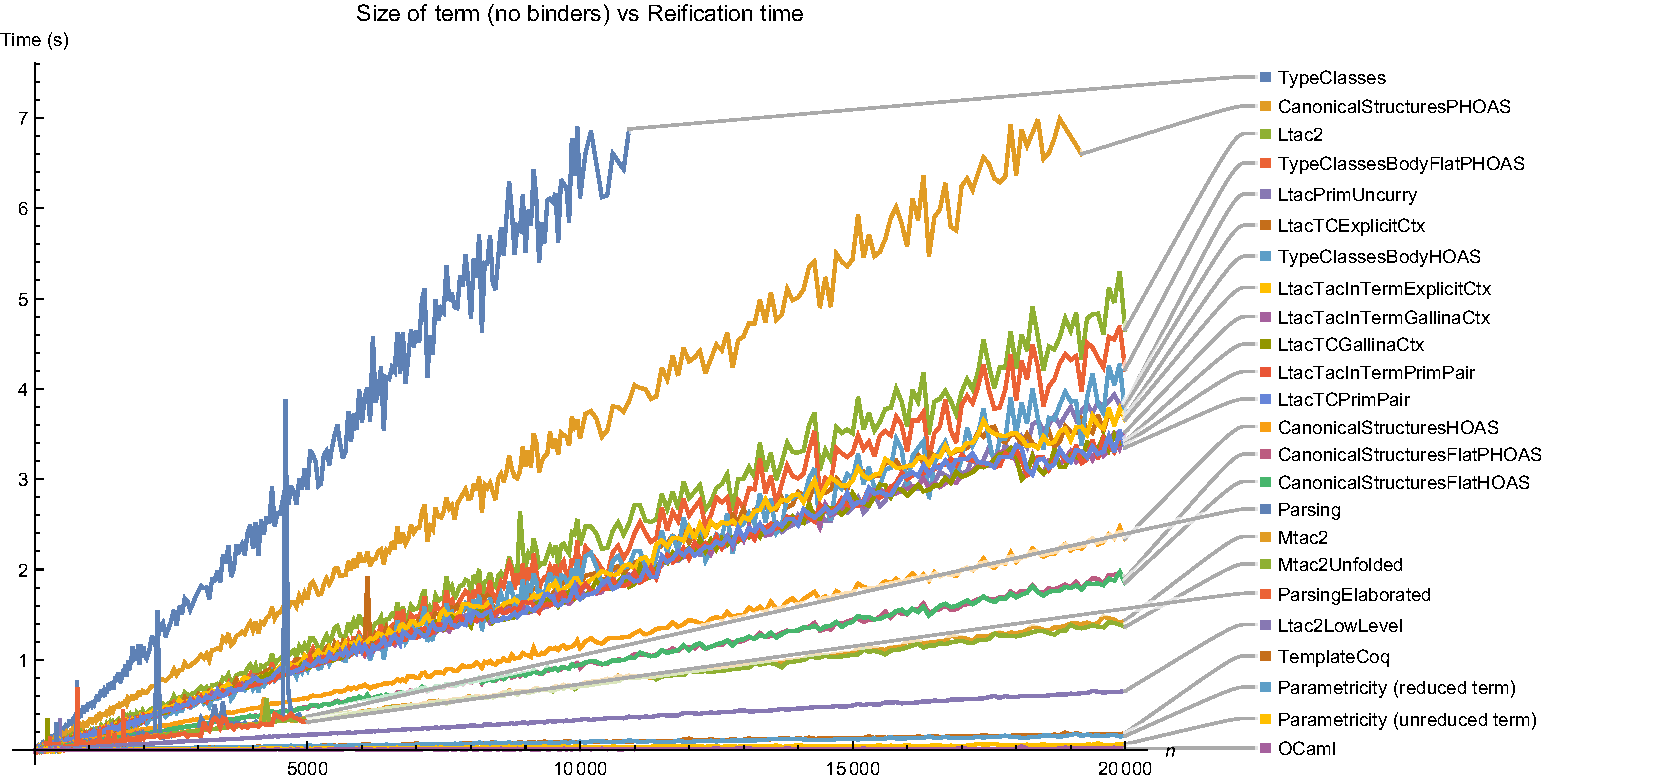
\includegraphics[width=\textwidth]{reification-by-parametricity-outputs/actual-reif-no-binders.pdf}
\caption{Performance of Reification without Binders}\label{fig:graph-reif-no-binders}
\end{figure}

Sorted from slowest to fastest, most of the labels in \autoref{fig:graph-reif-no-binders} should be self-explanatory and are found in similarly named \texttt{.v} files in the associated code; we call out a few potentially confusing ones:
\begin{itemize}
  \item
    The ``Parsing'' benchmark is ``reification by copy-paste'': a script generates a \texttt{.v} file with notation for an already-reified term; we benchmark the amount of time it takes to parse and typecheck that term.
    The ``ParsingElaborated'' benchmark is similar, but instead of giving notation for an already-reified term, we give the complete syntax tree, including arguments normally left implicit.
    Note that these benchmarks cut off at around 5000 rather than at around 20\,000, because on large terms, Coq crashes with a stack overflow in parsing.
    %For size reasons, we do not include these \texttt{.v} files in the associated code tarball, but they can be made via the \texttt{parsing-test-files} target, which generates some files in \texttt{Benchmarks/}.
%  \item
%    In \autoref{sec:ltac2-reif} we mention both a naïve transcription of \Ltac1 to \Ltac2 and a procedure using low-level primitives in \Ltac2; ``Ltac2'' benchmarks the former, and ``Ltac2LowLevel'' benchmarks the latter.
  \item
    We have four variants starting with ``CanonicalStructures'' here.
    The Flat variants reify to \texttt{@expr nat} rather than to \texttt{forall var, @expr var} and benefit from fewer function binders and application nodes.
    The HOAS variants do not include a case for \letindots\space nodes, while the PHOAS variants do.
    Unlike most other reification methods, there is a significant cost associated with handling more sorts of identifiers in canonical structures.
\end{itemize}

We note that on this benchmark our method is slightly faster than template-coq, which reifies to de Bruijn indices, and slightly slower than the quote plugin in the standard library\footnote{This plugin no longer appears in this graph because it was removed in Coq 8.10~\cite{coq-pr-remove-quote-plugin}, though it appears in the graph in \textcite{reification-by-parametricity}.} and the OCaml plugin we wrote by hand.

\subsection{With Binders} \label{sec:perf:binders}

We look at terms of the form \texttt{dlet a$_1$ := 1 * 1 in dlet a$_2$ := a$_1$ * a$_1$ in \ldots\space dlet a$_n$ := a$_{n-1}$ * a$_{n-1}$ in a$_n$}, where $n$ is the size of the term.
The first graph shown here includes all of the reification variants at linear scale, while the next step zooms in on the highest-performance variants at log-log scale.

\begin{figure}[t]
\noindent 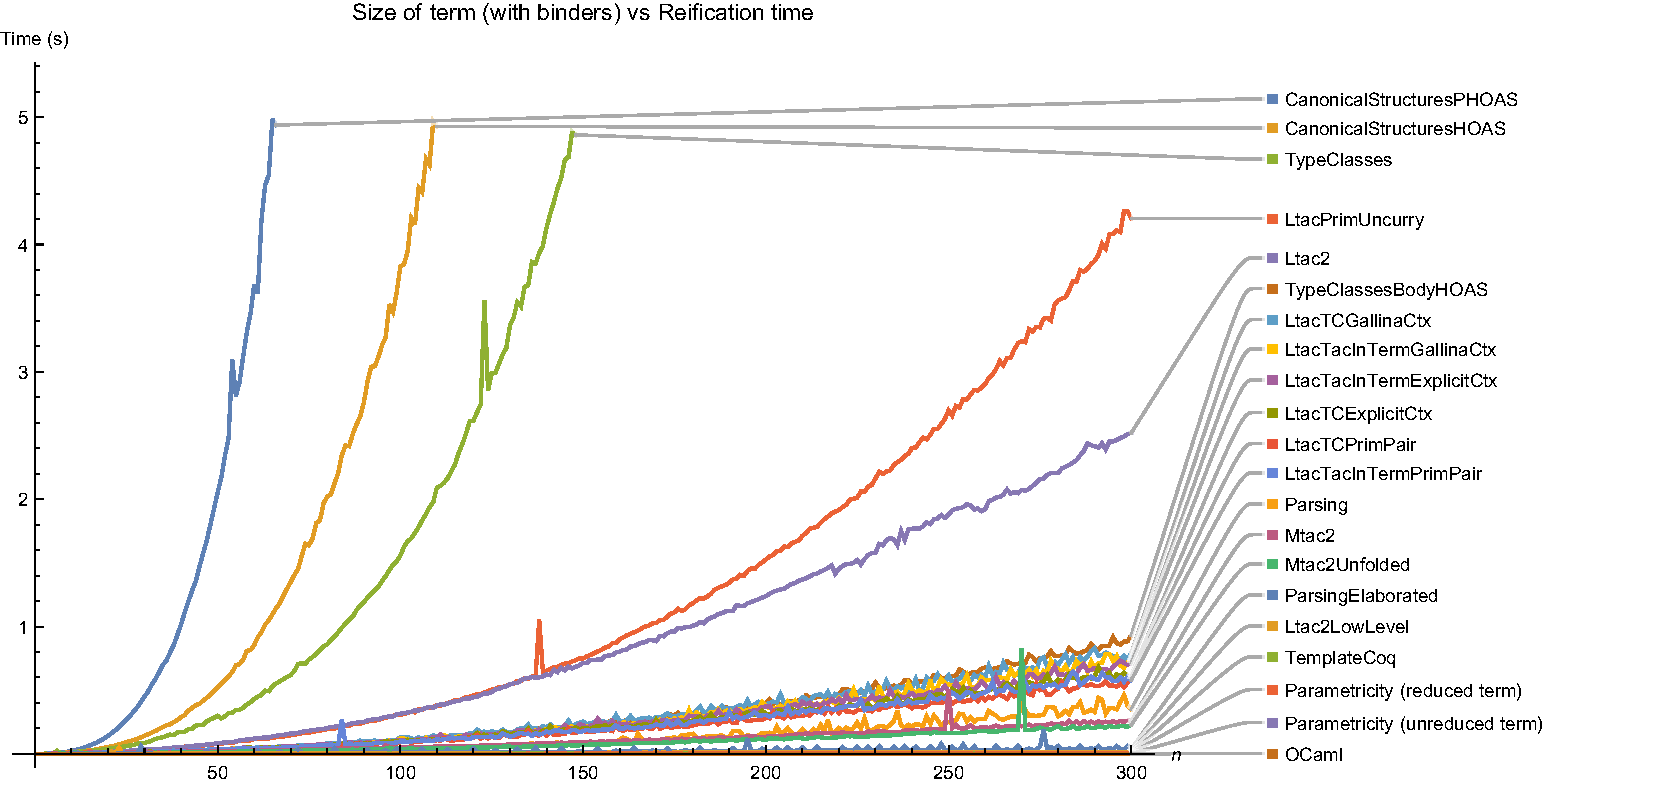
\includegraphics[width=\textwidth]{reification-by-parametricity-outputs/actual-reif-with-binders.pdf}

\noindent 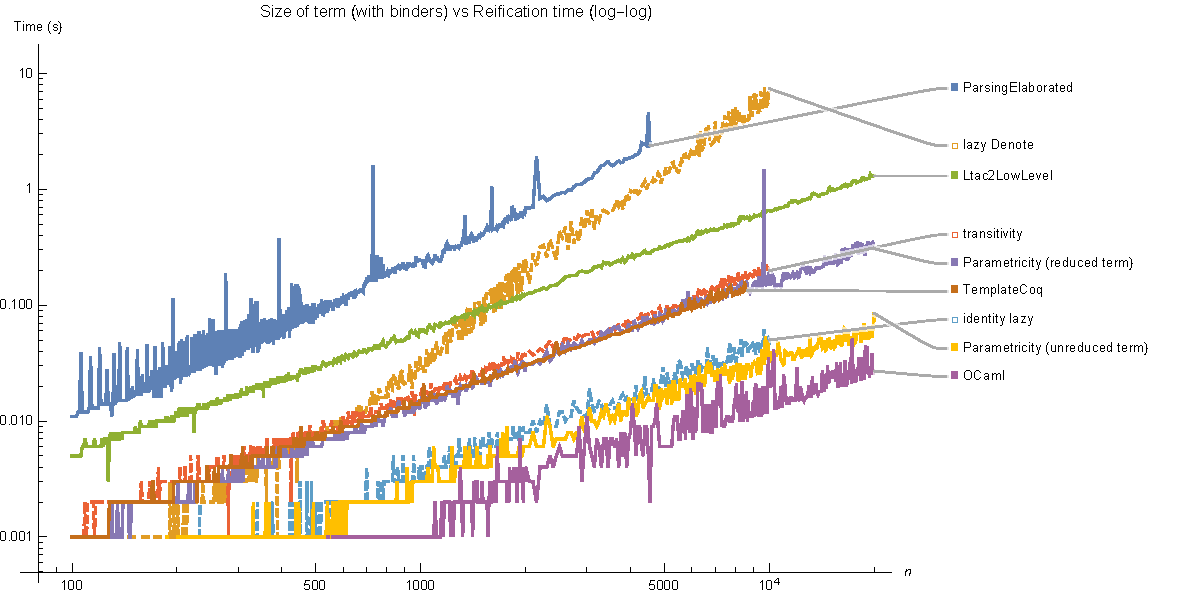
\includegraphics[width=\textwidth]{reification-by-parametricity-outputs/actual-reif-with-binders-log-log-subset.pdf}
\caption{Performance of Reification with Binders}\label{fig:reif-binders}
\end{figure}

In addition to reification benchmarks, the graph in \autoref{fig:reif-binders} includes as a reference (1) the time it takes to run \texttt{lazy} reduction on a reified term already in normal form (``identity lazy'') and (2) the time it takes to check that the reified term matches the original native term (``lazy Denote'').
The former is just barely faster than OCaml reification; the latter often takes longer than reification itself.
The line for the template-coq plugin cuts off at around 10\,000 rather than around 20\,000 because at that point template-coq starts crashing with stack overflows.

\todo{is this still true?}
A nontrivial portion of the cost of ``Parametricity (reduced term)'' seems to be due to the fact that looking up the type of a binder is linear in the number of binders in the context, thus resulting in quadratic behavior of the retyping step that comes after abstraction in the \texttt{pattern} tactic.
In Coq 8.8, this lookup is $\log n$, and so reification has become even faster than the plots indicate~\cite{coq-pr-fast-rel-lookup}.

\section{Future Work, Concluding Remarks} \label{sec:future}

We identify one remaining open question with this method that has the potential of removing the next largest bottleneck in reification: using reduction to show that the reified term is correct.

\begin{wrapfigure}[11]{r}{9cm}
%\vspace{-36pt}
\[
\xymatrix@R=0.5em@C=0em{
    \txt{unreduced term} \ar[d]^{\delta} \\
    \txt{small partially \\ reduced term}
    \ar@<1ex>[ddr]
    \ar@<-1ex>@{--}[rr]
    &&
    \txt{unreduced \\ reified syntax}
    \ar@<-1ex>@{--}[ll]^{???}
    \ar@<1ex>[ddl]
    \\ \\
    &
    \txt{unreduced \\ abstracted term}
    \ar@<1ex>[uul]
    \ar@<1ex>[uur]%^{\rotatebox{40}{\llap{\text{application\hspace*{-2em}}}}}
}
\]
%\vspace{-18pt}
\caption{Completing the commutative triangle}\label{fig:reify-denote-parametricity}
\end{wrapfigure}
Recall our reification procedure and the associated diagram, from \autoref{sec:expanded-reif-diagram}.
We perform $\delta$ on an unreduced term to obtain a small, partially reduced term;
we then perform abstraction to get an abstracted, unreduced term, followed by application to get unreduced reified syntax.
These steps are all fast.
Finally, we perform $\beta\iota$-reduction to get reduced, reified syntax and perform $\beta\iota\delta$ reduction to get back a reduced form of our original term.
These steps are slow, but we must do them if we are to have verified reflective automation.

It would be nice if we could prove this equality without ever reducing our term.
That is, it would be nice if we could have the diagram in \autoref{fig:reify-denote-parametricity}.

The question, then, is how to connect the small partially reduced term with \texttt{denote} applied to the unreduced reified syntax.
That is, letting $F$ denote the unreduced abstracted term, how can we prove, without reducing $F$, that
\[
F\ \mathbb{N}\ \text{Mul}\ \text{O}\ \text{S}\ (\text{@Let\_In }\mathbb{N}\texttt{ }\mathbb{N})
=
\texttt{denote}\ \left(F\ \texttt{expr}\ \texttt{NatMul}\ \texttt{NatO}\ \texttt{NatS}\ \texttt{LetIn}\right)
\]

We hypothesize that a form of internalized parametricity would suffice for proving this lemma.
In particular, we could specialize the type argument of $F$ with $\mathbb N \times \texttt{expr}$.
Then we would need a proof that for any function $F$ of type
\[
\forall (T : \texttt{Type}), (T \to T \to T) \to T \to (T \to T) \to (T \to (T \to T) \to T) \to T
\]
and any types $A$ and $B$, and any terms $f_A : A \to A \to A$, $f_B : B \to B\to B$, $a : A$, $b : B$, $g_A : A \to A$, $g_B : B \to B$, $h_A : A \to (A \to A) \to A$, and $h_B : B \to (B \to B) \to B$, using $f\times g$ to denote lifting a pair of functions to a function over pairs:
\begin{align*}
  & \texttt{fst}\ \left(F\ (A \times B)\ (f_A \times f_B)\ (a, b)\ (g_A \times g_B)\ (h_A \times h_B)\right) = F\ A\ f_A\ a\ g_A\ h_A \;\wedge \\
  & \texttt{snd}\ \left(F\ (A \times B)\ (f_A \times f_B)\ (a, b)\ (g_A \times g_B)\ (h_A \times h_B)\right) = F\ B\ f_B\ b\ g_B\ h_B
\end{align*}
This theorem is a sort of parametricity theorem.

Despite this remaining open question, we hope that our performance results make a strong case for our method of reification; it is fast, concise, and robust.

\part{Conclusion}\label{part:conclusion}
\chapter{\readyforreading{A Retrospective on Performance Improvements}}\label{ch:coq-tooling-fixes}\label{ch:retrospective}
Throughout this thesis, we've looked at the problem of performance in proof assistants, especially those based on dependent type theory, with Coq as our primary tool under investigation.
\autoref{part:introduction} aimed to convince the reader that this problem is interesting, important, challenging, and understudied, as it differs in non-trivial ways from performance bottlenecks in non-dependently-typed languages.
\autoref{part:design} discussed design principles to avoid performance pitfalls, and \autoref{part:rewriting} took a deep dive into a particular set of performance bottlenecks and presented a tool, and, we hope, exposed the underlying design methodology, that allows eliminating asymptotic bottlenecks in one important part of proof assistant systems.

In this chapter, we will look instead at the successes of the past decade\footnote{%
  Actually, the time span we're considering is the course of the author's experience with Coq, which is a bit less than a decade.%
}%
, ways in which performance has improved in major ways.
\autoref{sec:fixes:minutiae} will discuss specific improvements in the implementation of Coq which resulted in performance gains, paying special attention to the underlying bottleneck being addressed.
Those without special interest in the low-level details of proof assistant implementation may want to skip to \autoref{sec:fixes:coq-theory}, which will discuss changes to the underlying type theory of Coq which make possible drastic performance improvements.
While we will again have our eye on Coq in \autoref{sec:fixes:coq-theory}, we will broaden our perspective in \autoref{sec:fixes:theory} to discuss new discoveries of the past decade or so in dependent type theory which enable performance improvements but have not yet made their way into Coq.

\section{Concrete Performance Advancements in Coq}\label{sec:fixes:minutiae}
In this section, we dive into the minutiae: concrete changes to Coq that have measurably increased performance.
\subsection{Removing Pervasive Evar Normalization}\label{sec:econstr}
Back when I started using Coq, in version 8.4, almost every single tactic was at least linear in performance in the size of the goal.
This included tactics like ``add new hypothesis to the context of type \mintinline{coq}{True}'' (\mintinline{coq}{pose proof I}) and tactics like ``give me the type of the most recently added hypothesis'' (\mintinline{coq}{match goal with H : ?T |- _ => T end}).
The reason for this was pervasive \emph{evar normalization}.

Let us review some details of the way Coq handles proof scripts.
\minortodo{if this is described earlier, refer back to it}
Coq a partial proof term, where not-yet-given subterms are \emph{existential variables}, or evars, which may show up as goals.
For example, when proving the goal \mintinline{coq}{True ∧ True}, after running \mintinline{coq}{split}, the proof term would be \mintinline{coq}{conj ?Goal1 ?Goal2}, where \mintinline{coq}{?Goal1} and \mintinline{coq}{?Goal2} are evars.
There are two subtleties:
\begin{enumerate}
\item
  Evars may be under binders.
  Coq uses a locally nameless representation of terms (c.f.~\autoref{sec:binders:locally-nameless}), where closed terms use de Bruijn indices, but open terms, i.e., evars, refer to the variables in their context by name.
  Hence each evar carries with it a named context, which causes a great deal of trouble as described in \fullnameref{sec:perf:quadratic-evar-subst}.
\item
  Coq supports backtracking, so we must remember the history of partial proof terms.
  In particular, we cannot simply mutate partial proof terms to instantiate the evars, and copying the entire partial proof term just to update a small part of it would also incur a great deal of overhead.
  Instead, Coq never mutates the terms, and instead simply keeps a map of which evars have been instantiated with which terms, called the \emph{evar map}.
\end{enumerate}

There is an issue with the straightforward implementation of evars and evar maps.
When walking terms, care must be taken with the evar case, to check whether or not the evar has in fact been instantiated or not.
Subtle bugs in unification and other areas of Coq resulted from some functions being incorrectly sensitive to whether or not a term had been built via evar instantiation or given directly.%
\footnote{%
  See the discussion at \textcite{coq-pr-econstr} for more details.%
}
The fast-and-easy solution used in older versions of Coq was to simply evar-normalize the goal before walking it.
That is, every tactic that had to walk the goal for any reason whatsoever would create a copy of the type of the goal---and sometimes the proof context as well---replacing all instantiated evars with their instantiation.
Needless to say, this was very expensive when the size of the goal was large.

\minortodo{include performance graphs?}

As of Coq 8.7, most tactics no longer perform useless evar normalization, and instead walk terms using a dedicated API which does on-the-fly normalization as necessary~\cite{coq-pr-econstr}.
This brought speedups of over 10\% to some developments, and improved asymptotic performance of some tactic scripts and interactive proof development.

\subsection{Delaying the Externalization of Application Arguments}\label{sec:delayed-externalization}
Coq has many representations of terms.
There is \texttt{constr\_expr}, the AST produced by Coq's parser.
Internalization turns \texttt{constr\_expr} into the untyped \texttt{glob\_constr} representation of terms by performing name resolution, bound variable checks, notation desugaring, and implicit argument insertion~\cite{Constrintern}.
Type inference fills in the holes in untyped \texttt{glob\_constr}s to turn them into typed \texttt{constr}s, possibly with remaining existential variables~\cite{Pretyping}.
In order to display proof goals, this process must be reversed.
The internal representation of \texttt{constr} must be ``detyped'' into \texttt{glob\_constr}s, which involves primarily just turning de Bruijn indices into names~\cite{Detyping}.
Finally, implicit arguments must be erased and notations must be re-sugared when externalizing \texttt{glob\_constr}s into \texttt{constr\_expr}s, which can be printed relatively straightforwardly~\cite{Constrextern,Ppconstr}.

In old versions, Coq would externalize the entire goal, including subterms that were never printed due to being hidden by notations and implicit arguments.
Starting in version 8.5pl2, lazy externalization of function arguments was implemented~\cite{coq-commit-delayed-externalization}.
This resulted in massive speed-ups to interactive development involving large goals whose biggest subterms were mostly hidden.

Changes like this one can be a game-changer for interactive proof development.
The kind of development that can happen when it takes a tenth of a second to see the goal after executing a tactic is vastly different from the kind of development that can happen when it takes a full second or two.
In the former case, the proof engine can almost feel like an extension of the coder's mind, responding to thoughts about strategies to try almost as fast as they can be typed.
In the latter case, development is significantly more clunky and involves much more friction.

In the same vein, bugs such as \coqbug{3691} and \coqbug{4819}, where Coq crawled the entire evar map in \texttt{-emacs} mode (used for ProofGeneral/Emacs) looking at all instantiated evars, resulted in interactive proof times of up to half-a-second for every goal display, even when the goal was small and there was nothing in the context.
Fixed in Coq 8.6, these bugs, too, got in the way of seamless proof development.

\subsection{The \Ltac\space Profiler}\label{sec:ltac-prof}
\begin{quote}
  If you blindly optimize without profiling, you will likely waste your time on the 99\% of code that isn't actually a performance bottleneck and miss the 1\% that is.
\end{quote}
\begin{flushright}
  --- Charles E.~Leiserson\footnote{%
Although this quote comes from the class I took at MIT, 6.172 --- Performance Engineering of Software Systems, the inspiration for the quote is an extended version of Donald Knuth's ``premature optimization is the root of all evil'' quote:
\begin{quote}
  Programmers waste enormous amounts of time thinking about, or worrying about, the speed of noncritical parts of their programs, and these attempts at efficiency actually have a strong negative impact when debugging and maintenance are considered.
  We \emph{should} forget about small efficiencies, say about 97\% of the time: premature optimization is the root of all evil.
  Yet we should not pass up our opportunities in that critical 3\%.
\end{quote}
\begin{flushright}
  --- Donald E.~Knuth~\cite[p.~268]{KnuthPrematureOptimizationExtended}
\end{flushright}%
}%
~\cite{Profiling2020Leiserson}
\end{flushright}

In old versions of Coq, there was no good way to profile tactic execution.
Users could wrap some invocations in \mintinline{coq}{time} to see how long a given tactic took, or could regularly print some output to see where execution hung.
Both of these are very low-tech methods of performance debugging, and work well enough for small tactics.
For debugging hundreds or thousands of lines of \Ltac\space code, though, these methods are insufficient.

A genuine profiler for \Ltac\space was developed in 2015 and integrated into Coq itself in version 8.6~\cite{coqpl-15-ltac-profiler}.

For those interested in amusing quirks of implementation details, the profiler itself was relatively easy to implement.
If I recall correctly, Tobias Tebbi, after hearing of my \Ltac\space performance woes, mentioned to me the profiler he implemented over the course of a couple of days.
Since \Ltac\space already records backtraces for error reporting, it was a relatively simple matter to hook into the stack-trace-recorder and track how much time was spent in each call-stack.
With some help from the Coq development team, I was able to adapt the patch to the new tactic engine of Coq $\ge$ 8.5, and shepherded it into Coq's codebase.

\minortodo{should I include more text here, extracting from the abstract submitted to CoqPL?}

\subsection{Compilation to Native Code}\label{sec:native-compiler}
Starting in version 8.5, Coq allows users to compile their functional Gallina programs to native code and fully reduce them to determine their output~\cite{nativecompute,coq-commit-native-compiler}.
In some cases, the native compiler is almost $10\times$ faster%
\footnote{\url{https://github.com/coq/coq/pull/12405\#issuecomment-633612308}}
than the optimized call-by-value evaluation bytecode-based virtual machine described in \textcite{vmcompute}.

The native compiler shines most at optimizing algorithmic and computational bottlenecks.
For example, computing the number of primes less than $n$ via the Sieve of Eratosthenes is about $2\times$ to $5\times$ faster in the native compiler than in the VM.
\minortodo{should I include code and/or plots?}
By contrast, when the input term is very large compared to the amount of computation, the compilation time can dwarf the running time, eating up any gains that the native compiler has over the VM.
This can be seen by comparing the times it takes to get the head of the explicit list of all unary-encoded natural numbers less than, say, 3000, on which the native compiler (1.7s) is about 5\% slower than the VM (1.6s) which itself is about $2\times$ slower than built-in call-by-value reduction machine (0.79s) which requires no translation.
Furthermore, when the output is large, both the VM and the native compiler suffer from inefficiencies in the readback code.
\minortodo{should I add an example or plots?}
%Fixpoint walk {A} (ls : list A) : unit := match ls with nil => tt | cons _ xs => walk xs end.
%Time Check ltac:(restart_timer;
%                let v := (eval vm_compute in (walk (seq 0 (Z.to_nat 2000)))) in
%                finish_timing ("Tactic call 1(vm)");
%                restart_timer;
%                let v := (eval native_compute in (walk (seq 0 (Z.to_nat 2000)))) in
%                finish_timing ("Tactic call 1(native)");
%                let v := (eval vm_compute in (seq 0 3000)) in
%                restart_timer;
%                let __ := (eval lazy in (List.hd 0%nat v)) in
%                finish_timing ("Tactic call 2(lazy)");
%                restart_timer;
%                let __ := (eval cbv in (List.hd 0%nat v)) in
%                finish_timing ("Tactic call 2(cbv)");
%                restart_timer;
%                let __ := (eval native_compute in (List.hd 0%nat v)) in
%                finish_timing ("Tactic call 2(native)");
%                restart_timer;
%                let __ := (eval vm_compute in (List.hd 0%nat v)) in
%                finish_timing ("Tactic call 2(vm)");
%                exact 0).


\minortodo{Should I add more to this section?  What should I say?}

\subsection{Primitive Integers and Arrays}\label{sec:prim-ints-arrays}
Primitive 31-bit integer arithmetic operations were added to Coq in 2007~\cite{coq-commit-int31,Extending2010Armand}.
Although most of Coq merely used an inductive representation of 31-bit integers, the VM included code for compiling these constants to native machine integers.%
\footnote{%
  The integer arithmetic is 31-bit rather than 32-bit because OCaml reserves the lowest bit for tagging whether a value is a pointer address to a tagged value or an integer.%
}
After hitting memory limits in storing the inductive representations in proofs involving proof traces from SMT solvers, work was started to allow the use of primitive datatypes that would be stored efficiently in proof terms~\cite{denes2013prim-ints-arrays}.

Some of this work has since been merged into Coq, including IEEE 754-2008 binary64 floating point numbers merged in Coq 8.11~\cite{coq-pr-floats}, 63-bit integers merged in Coq 8.10~\cite{coq-pr-int63}, and persistent arrays~\cite{Persistent2007Conchon} merged into Coq 8.13~\cite{coq-pr-parray}.
Work enabling primitive recursion over these native datatypes is still underway,~\cite{coq-pr-parray-prim-recursion} and the actual use of these primitive datatypes to reap the performance benefits is still to come as of the writing of this thesis.

\subsection{Primitive Projections for Record Types}\label{sec:fixes:theory:primitive-projections}\label{sec:primitive-projections}
Since version 8.5, Coq has had the ability to define record types with projections whose arguments are not stored in the term representation~\cite{coq-commit-polyproj}.
This allows asymptotic speedups, as discussed in \fullnameref{sec:prim-record-proj}.
\minortodo{what should be said in this section?}

Note that this is a specific instance of a more general theory of implicit arguments~\cite{logical2001implicit,barras2008implicit}, and there has been other work on how to eliminate useless arguments from term representations~\cite{Inductive2003Brady}.

\subsection{Fast Typing of Application Nodes}
In \fullnameref{sec:perf:quadratic-application}, we discussed how the typing rule for function application resulted in quadratic performance behavior when there was in fact only linear work that needed to be done.
As of Coq 8.10, when typechecking applications in the kernel, substitution is delayed so as to achieve linear performance~\cite{coq-pr-fast-application-typing}.
\minortodo{does this need more of a recap?}
Unfortunately, the pretyping and type inference algorithm is still quadratic, due to the type theory rules used for type inference.

\minortodo{should I talk about https://github.com/coq/coq/pull/263 - Fast lookup in named contexts?}
\minortodo{should I talk about https://github.com/coq/coq/pull/6506 - Fast rel lookup?}

\section{Performance-Enhancing Advancements in the Type Theory of Coq}\label{sec:fixes:coq-theory}
While some of the above performance enhancements touch the trusted kernel of Coq, they do not fundamentally change the type theory.
Some performance enhancements require significant changes to the type theory.
In this section we will review a couple of particularly important changes of this kind.

\subsection{Universe Polymorphism}\label{sec:fixes:theory:univ-poly}\label{sec:univ-poly}

Recall that the main case study of \autoref{ch:design} was our implementation of a category theory library.
Recall also from \nameref{sec:abstraction-barriers:packed-records} how the choice of whether to use packed or unpacked records impacts performance; while unpacked records are more friendly for developing algebraic hierarchies, packed records achieve significantly better performance when large towers of dependent concepts (such as categories, functors between categories, and natural transformations between functors) are formalized.

This section addresses a particular feature which allows an entire-library $2\times$ speed-up when using fully-packed records.
How is such a large performance gain achievable?
Without this feature, called \emph{universe polymorphism}, encoding some mathematical objects requires \emph{duplicating} the entire library!
Removing this duplication of code will halve the compile-time.

\subsubsection{What are universes?}\label{sec:universes-def}
Universes are type theory's answer to Russell's paradox~\cite{sep-russell-paradox}.
Russell's paradox, a famous paradox discovered in 1901, proceeds as follows.
A \emph{set} is an unordered collection of distinct objects.
Since each \emph{set} is an object, we may consider the set of all sets.
Does this set contain itself?
It must, for by definition it contains all sets.

So we see by example that some sets contain themselves, while others (such as the empty set with no objects) do not.
Let us consider now the set consisting of exactly the sets that do not contain themselves.
Does this set contain itself?
If it does not, then it fails to live up to its description as the set of \emph{all} sets that do not contain themselves.
However, if it does contain itself, then it also fails to live up to its description as a set consisting \emph{only} of sets that do not contain themselves.
Paradox!

The resolution to this paradox is to forbid sets from containing themselves.
The collection of all sets is too big to be a set, so let's call it (and collections of its size) a proper class.
We can nest this construction, as type theory does:
We have \mintinline{coq}{Type₀}, the \mintinline{coq}{Type₁} of all small types, and we have \mintinline{coq}{Type₁}, the \mintinline{coq}{Type₂} of all \mintinline{coq}{Type₁}s, etc.
These subscripts are called \emph{universe levels}, and the subscripted \mintinline{coq}{Type}s are sometimes called \emph{universes}.

Most constructions in Coq work just fine if we simply place them in a single, high-enough, universe.
In fact, the entire standard library in Coq effectively uses only three universes.
Most of the standard library in fact only needs one universe.
We need a second universe for the few constructions that talk about equality between types, and a third for the encoding of a variant of Russell's paradox in Coq.

However, one universe is not sufficient for category theory, even if we don't need to talk about equality of types nor prove that \mintinline{coq}{Type : Type} is inconsistent.

The reason is that category theory, much like set theory, talks about itself.
\minortodo{check if category has been defined before}

\subsubsection{Complications from Categories of Categories}\label{sec:category-def}\label{sec:category-of-categories}

In standard mathematical practice, a category \cat{C} can be defined~\cite{awodey2010category} to consist of:
\begin{itemize}
  \item
    a class \Ob[C] of \emph{objects}
  \item
    for all objects $a, b \in \Ob[C]$, a class $\Hom[C](a, b)$ of \emph{morphisms from $a$ to $b$}
  \item
    for each object $x \in \Ob[C]$, an \emph{identity morphism} $\Id[x] \in \Hom[C](x, x)$
  \item
    for each triple of objects $a, b, c \in \Ob[C]$, a \emph{composition function} $\circ : \Hom[C](b, c) \times \Hom[C](a, b) \to \Hom[C](a, c)$
\end{itemize}
satisfying the following axioms:
\begin{itemize}
  \item
    associativity: for composable morphisms $f$, $g$, $h$, we have $f \circ (g \circ h) = (f \circ g) \circ h$.
  \item
    identity: for any morphism $f \in \Hom[C](a, b)$, we have $\Id[b] \circ f = f = f \circ \Id[a]$
\end{itemize}

Some complications arise in applying the last subsection's definition of categories to the full range of common constructs in category theory.
One particularly prominent example formalizes the structure of a collection of categories, showing that this collection itself may be considered as a category.

The morphisms in such a category are \emph{functors},\label{sec:define-functor} maps between categories consisting of a function on objects, a function on hom-types, and proofs that these functions respect composition and identity~\cite{mac1998categories,awodey2010category,HoTTBook}.

The naïve concept of a ``category of all categories'',\label{sec:category-of-categories} which includes even itself, leads into mathematical inconsistencies which manifest as universe inconsistency errors in Coq, much as with the set of all sets discussed above.

The standard resolution, as with sets, is to introduce a hierarchy of categories, where, for instance, most intuitive constructions are considered \emph{small} categories, and then we also have \emph{large} categories, one of which is the category of small categories.
Both definitions wind up with literally the same text in Coq, giving:
\begin{minted}{coq}
Definition SmallCat : LargeCategory :=
  {| Ob := SmallCategory;
     Hom C D := SmallFunctor C D;
     ⋮
  |}.
\end{minted}

It seems a shame to copy-and-paste this definition (and those of \mintinline{coq}{Category}, \mintinline{coq}{Functor}, etc.) $n$ times to define an $n$-level hierarchy.

\emph{Universe polymorphism}\label{sec:universe-polymorphism-def} is a feature that allows definitions to be quantified over their universes.
While Coq 8.4 supports a restricted flavor of universe polymorphism that allows the universe of a definition to vary as a function of the universes of its arguments, Coq 8.5 and later~\cite{coq-commit-polyproj} support an established kind of more general universe polymorphism~\cite{Harper1991107}, previously implemented only in \NuPRL~\cite{nuprl}.
In these versions of Coq, any definitions declared polymorphic are parametric over their universes.

While judicious use of universe polymorphism can reduce code duplication, careless use can lead to tens of thousands of universe variables which then become a performance bottleneck in their own right.%
\footnote{%
  See, for example, the commit message of \githubref[][ in the HoTT/HoTT library on GitHub]{HoTT/HoTT}{a445bc38c172a8f2787afe7d9d193596a0f6e1bd}, where moving from Coq 8.5$\beta$2 to 8.5$\beta$3 incurred a 4$\times$ slowdown in the file \texttt{hit/V.v}, entirely due to performance regressions in universe handling, which were later fixed.
  This slowdown is likely the one of \coqbug{4537}.

  See also \githubref[commit ][ in the HoTT/HoTT library on GitHub]{HoTT/HoTT}{d499ef667f1cf90c0886c906dd1780eae93a3046}, where reducing the number of polymorphic universes in some constants used by \texttt{rewrite} resulted in an overall $2\times$ speedup, with speedups reaching $10\times$ in some \texttt{rewrite}-heavy files.

  Coq actually had an implementation of full universe polymorphism between versions 8.3 and 8.4, implemented in \githubref[commit ]{coq/coq}{d98dfbcae463f8d699765e2d7004becd7714d6cf} and reverted mere minutes later in \githubref[commit ]{coq/coq}{60bc3cbe72083f4fa1aa759914936e4fa3d6b42e}.
  In-person discussion, either with Matthieu himself or with Bob Harper, revealed that Matthieu abandoned this initial attempt after finding that universe polymorphism was too slow, and it was only by implementing the algorithm of \textcite{Harper1991107} that universe polymorphism with typical ambiguity~\cite{Universe2012Shulman,Typical1966Specker,Harper1991107}, where users need not write universe variables explicitly, was able to be implemented in a way that was sufficiently performant.%
}

\subsection{Judgmental η for Record Types}\label{sec:fixes:theory:record-eta}\label{sec:record-eta}
The same commit that introduced universe polymorphism in Coq 8.5 also introduced judgmental $\eta$ conversion for records with primitive projections~\cite{coq-commit-polyproj}.
We have already discussed the advantages of primitive projections in \autoref{sec:primitive-projections}, and we have talked a bit about judgmental $\eta$ in \fullnameref{sec:no-judgmental-eta} and \fullnameref{sec:duality-conversion}.

\minortodo{make sure we've talked about judgmental equality and conversion}
The $\eta$ conversion rule for records says that every term $x$ of record type $T$ is convertible with the constructor of $T$ applied to the projections of $T$ applied to $x$.
For example, if \mintinline{coq}{x} has type \mintinline{coq}{A * B}, then the $\eta$ rule equates \mintinline{coq}{x} with \mintinline{coq}{(fst x, snd x)}.

As discussed in \autoref{sec:duality-conversion}, having records with judgmental $\eta$ conversion allows de-duplicating code that would otherwise have to be duplicated.
\minortodo{should more be said here?}

\subsection{SProp: The Definitionally Proof Irrelevant Universe}\label{sec:fixes:theory:sprop}\label{sec:sprop}
We discussed in \fullnameref{sec:term-size} how irrelevant proof arguments tended to cause performance issues just by existing as part of the goal.
While there is as-yet no way to erase these arguments, Coq versions 8.10 and later have the ability to define types as judgmentally irrelevant, paving the way for more aggressive erasure~\cite{coq-pr-sprop,sprop}.
\minortodo{should more be said here?}

\section{Performance-Enhancing Advancements in Type Theory at Large}\label{sec:fixes:theory}
We come now to discoveries and inventions of the past decade or so which have not yet made it into Coq but which show great promise for significant performance improvements.

\subsection{Higher Inductive Types: Setoids for Free}\label{sec:fixes:theory:HITs}\label{sec:HITs}
\minortodo{is this sentence redundant?}
\minortodo{fix the intro to this subsection}
\minortodo{fix flow}
Recall again that the main case study of \autoref{ch:design} was our implementation of a category theory library.

\subsubsection{Equality}\label{sec:equality}
Equality, which has recently become a very hot topic in type theory~\cite{HoTTBook} and higher category theory~\cite{Leinster2007}, provides another example of a design decision where most usage is independent of the exact implementation details.
Although the question of what it means for objects or morphisms to be equal does not come up much in classical 1-category theory, it is more important when formalizing category theory in a proof assistant, for reasons seemingly unrelated to its importance in higher category theory.
We consider some possible notions of equality.

\paragraph{Setoids}
A setoid~\cite{bishop1967foundations} is a carrier type equipped with an equivalence relation; a map of setoids is a function between the carrier types and a proof that the function respects the equivalence relations of its domain and codomain.
Many authors \cite{copumpkin/categories,MathClasses,megacz-coq-categories,huet2000constructive,benediktahrens/coinductives,ahrens2010categorical,konn/category-agda,Algebra,mattam82-cat,Carvalho1998,wilander2012constructing%
  %,rs-/triangles%
}
choose to use a setoid of morphisms, which allows for the definition of the category of set(oid)s, as well as the category of (small) categories, without assuming functional extensionality, and allows for the definition of categories where the objects are quotient types.
However, there is significant overhead associated with using setoids everywhere, which can lead to slower compile times.
Every type that we talk about needs to come with a relation and a proof that this relation is an equivalence relation.
Every function that we use needs to come with a proof that it sends equivalent elements to equivalent elements.
Even worse, if we need an equivalence relation on the universe of ``types with equivalence relations'', we need to provide a transport function between equivalent types that respects the equivalence relations of those types.

\paragraph{Propositional Equality}
An alternative to setoids is propositional equality, which carries none of the overhead of setoids, but does not allow an easy formulation of quotient types, and requires assuming functional extensionality to construct the category of sets.

\minortodo{check if we've defined propositional equality before}
Intensional type theories like Coq's have a built-in notion of equality, often called definitional equality or judgmental equality, and denoted as $x \equiv y$.
This notion of equality, which is generally internal to an intensional type theory and therefore cannot be explicitly reasoned about inside of that type theory, is the equality that holds between $\beta\delta\iota\zeta\eta$-convertible terms.

Coq's standard library defines what is called \emph{propositional equality} on top of judgmental equality, denoted $x = y$.
One is allowed to conclude that propositional equality holds between any judgmentally equal terms.

Using propositional equality rather than setoids is convenient because there is already significant machinery made for reasoning about propositional equalities, and there is much less overhead.
However, we ran into significant trouble when attempting to prove that the category of sets has all colimits, which amounts to proving that it is closed under disjoint unions and quotienting; quotient types cannot be encoded without assuming a number of other axioms.

\paragraph{Higher Inductive Types}\label{sec:hit}
The recent emergence of higher inductive types allows the best of both worlds.
 The idea of higher inductive types~\cite{HoTTBook} is to allow inductive types to be equipped with extra proofs of equality between constructors.
They originated as a way to allow homotopy type theorists to construct types with non-trivial higher paths.
A very simple example is the interval type, from which functional extensionality can be proven~\cite{interval-implies-funext}.
The interval type consists of two inhabitants \mintinline{coq}{zero : Interval} and \mintinline{coq}{one : Interval}, and a proof \mintinline{coq}{seg : zero = one}.
In a hypothetical type theory with higher inductive types, the type checker does the work of carrying around an equivalence relation on each type for us, and forbids users from constructing functions that do not respect the equivalence relation of any input type.
For example, we can, hypothetically, prove functional extensionality as follows:
\begin{minted}{coq}
Definition f_equal {A B x y} (f : A → B) : x = y → f x = f y.
Definition functional_extensionality {A B} (f g : A → B)
    : (∀ x, f x = g x) → f = g
  := λ (H : ∀ x, f x = g x)
       ⇒ f_equal (λ (i : Interval) (x : A)
                     ⇒ match i with
                         | zero ⇒ f x
                         | one  ⇒ g x
                         | seg  ⇒ H x
                       end)
                  seg.
\end{minted}
Had we neglected to include the branch for \mintinline{coq}{seg}, the type checker should complain about an incomplete match; the function \mintinline{coq}{λ i : Interval ⇒ match i with zero ⇒ true | one ⇒ false end} of type \mintinline{coq}{Interval → bool} should not typecheck for this reason.

The key insight is that most types do not need any special equivalence relation, and, moreover, if we are not explicitly dealing with a type with a special equivalence relation, then it is impossible (by parametricity) to fail to respect the equivalence relation.
Said another way, the only way to construct a function that might fail to respect the equivalence relation would be by some eliminator like pattern matching, so all we have to do is guarantee that direct invocations of the eliminator result in functions that respect the equivalence relation.

As with the choice involved in defining categories, using propositional equality with higher inductive types rather than setoids derives many of its benefits from not having to deal with all of the overhead of custom equivalence relations in constructions that do not need them.
In this case, we avoid the overhead by making the type checker or the metatheory deal with the parts we usually do not care about.
Most of our definitions do not need custom equivalence relations, so the overhead of using setoids would be very large for very little gain.

\subsection{Univalence and Isomorphism Transport}\label{sec:fixes:theory:univalence}\label{sec:univalence}
When considering higher inductive types, the question ``when are two types equivalent?'' arises naturally.
The standard answer in the past has been ``when they are syntactically equal''.
The result of this is that two inductive types that are defined in the same way, but with different names, will not be equal.
Voevodsky's univalence principle gives a different answer: two types are equal when they are isomorphic.
This principle, encoded formally as the \emph{univalence axiom}, allows reasoning about isomorphic types as easily as if they were equal.

\Citeauthor*{Equivalences2018Tabareau} built a framework on top of the insights of univalence, combined with parametricity~\cite{reynolds1983types,wadler1989theorems}, for automatically porting definitions and theorems to equivalent types~\cite{Equivalences2018Tabareau,Tabareau2019TheMO}.

What is the application to performance?
As we saw, for example, in \fullnameref{sec:rewriting-more:AST:choices}, the choice of representation of a datatype can have drastic consequences on how easy it is to encode algorithms and write correctness proofs.
These design choices can also be intricately entwined with both the compile-time and run-time performance characteristics of the code.
One central message of both \autoref{ch:rewriting-more} and \autoref{ch:design} is that picking the right API really matters when writing code with dependent types.
The promise of univalence, still in its infancy, is that we could pick the right API for each algorithmic chunk, prove the APIs isomorphic, and use some version of univalence to compose the APIs and reason about the algorithms as easily as if we had used the same interface everywhere.

\minortodo{should I talk about the difference between isomorphism and equivalence?}
\minortodo{what more should be said here?}

\subsection{Cubical Type Theory}\label{sec:fixes:theory:cubical}\label{sec:cubical}
One important detail we elided in the previous subsections is the question of computation.
Higher inductive types and univalence are much less useful if they are opaque to the type checker.
The proof of function extensionality, for example, relies on the elimination rule for the interval having a judgmental computation rule.%
\footnote{%
  We leave it as a fun exercise for the advanced reader to figure out why the Church encoding of the interval, where \mintinline{coq}{Interval := ∀ P (zero : P) (one : P) (seg : zero = one), P}, does not yield a proof a functional extensionality.%
}

\minortodo{define point vs path constructors}
Higher inductive types whose eliminators compute on the point constructors can be hacked into dependently-typed proof assistants by adding inconsistent axioms and then hiding them behind opaque APIs so that inconsistency cannot be proven~\cite{Running2011Licata,Bertot2013}.
This is unsatisfactory, however, on two counts:
\begin{enumerate}
\item
  The eliminators do not compute on path constructors.
  For example, the interval eliminator would compute on \mintinline{coq}{zero} and \mintinline{coq}{one}, but not on \mintinline{coq}{seg}.
\item
  Adding these axioms compromises the trust story.
\end{enumerate}

Cubical type theory is the solution to both of these problems, for both higher inductive types and univalence~\cite{Cubical2016Cohen}.
Unlike most other type theories, computation in cubical type theory is implemented by appealing to the category theoretic model, and the insights that allow such computation are slowly making their way into more mainstream dependently-typed proof assistants~\cite{Cubical2019Vezzosi}.

\begin{comment}
\begin{subappendices}
    \section{Fragments from the category theory paper}
    For reasons that we present in the course of the paper, we were unsatisfied with the feature set of released Coq version 8.4.  We wound up adopting the Coq version under development by homotopy type theorists~\cite{HoTT/coq}, making critical use of its stronger universe polymorphism (\autoref{sec:category-of-categories}) and higher inductive types (\autoref{sec:hit}).  We hope that our account here provides useful data points for proof assistant designers about which features can have serious impact on proving convenience or performance in very abstract developments.  The two features we mentioned earlier in the paragraph can simplify the Coq user experience dramatically, while a number of other features, at various stages of conception or implementation by Coq team members, can make proving much easier or improve proof script performance by orders of magnitude, generally by reducing term size (\autoref{sec:term-size}): primitive record projections (\autoref{sec:prim-record-proj}), internalized proof irrelevance for equalities (\autoref{sec:equality-reflection}), and $\eta$ rules for records (\autoref{sec:no-judgmental-eta}) and equality proofs (\autoref{sec:compute-match}).

    \hrule


\end{subappendices}
\end{comment}

\chapter{Concluding Remarks}\label{ch:conclusion}
%We come, at last, to the closing remarks of this dissertation.
%\todoac{This sentence seems hokey and at risk of conveying too little info, given the chapter title.}

We spent \autoref{part:introduction} mapping out the landscape of the problems of performance we encountered in dependently typed proof assistants.
In \autoref{part:rewriting} and \autoref{part:design}, we laid out more-or-less systematic principles and tools for avoiding these performance bottlenecks.
In the last chapter, \autoref{ch:retrospective}, we looked back on the concrete performance improvements in Coq over time.

We look now to the future.

The clever reader might have noticed something that we swept under the rug in \Autoref{part:rewriting,part:design}.
In \autoref{sec:intro:proof-assistant-design-choices} we laid out two basic design choices---dependent types and the de Bruijn criterion---which are responsible for much of the power and much of the trust we can have in a proof assistant like Coq.
We then spent the next chapters of this dissertation investigating the performance bottlenecks that can perhaps be said to result from these choices and how to ameliorate these performance issues.

If the strategies we laid out in \Autoref{part:rewriting,part:design} for how to use dependent types and untrusted tactics in a performant way are to be summed up in one word, that word is: ``don't!''
To avoid the performance issues resulting from tactics being untrusted, the source of much of the trust in proof assistants like Coq, we suggest in \autoref{part:rewriting} that users effectively \emph{throw away the entire tactic engine} and instead code tactics reflectively.
To avoid the performance issues incurred by unpredictable computation at the type level, the source of much of the power of dependent type theory, we broadly suggest in \autoref{part:design} to \emph{avoid using the computation at all} (except in the rare cases where the entire proof can be moved into computation at the type level, such as proof by duality (\autoref{sec:duality-conversion}) and proof by reflection (\autoref{ch:reflection})).

This is a sorry state of affairs:
we are effectively advising users to basically avoid using most of the power and infrastructure of the proof assistant.

We admit that we are not sure what an effective resolution to the performance issue of computation at the type level would look like.
While \autoref{ch:design} lays out in \fullnameref{sec:when-how-dependent-types} principles for how and when to use dependent types that allow us to recover much of the power of dependent types without running into issues of slow conversion, even at scale, this is nowhere near a complete roadmap for actually using partial computation at the type level.

On the question of using tactics, however, we do know what a resolution would look like, and hence we conclude this dissertation with such a call for future research.

As far as we can tell, no one has yet laid out a theory of what are the necessary basic building blocks of a usable tactic engine for proofs.
Such a theory should include:
\begin{itemize}
\item
  a list of basic operations
\item
  with necessary asymptotic performance,
\item
  justification that these building blocks are sufficient for constructing all the proof automation users might want to construct, and
\item
  justification that the asymptotic performance does not incur needless overhead above and beyond the underlying algorithm of proof construction.
\end{itemize}

What is \emph{needless} overhead, though?
How can we say what the performance of the ``underlying algorithm'' is?

A first stab might be thus: we want a proof engine which, for any heuristic algorithm $A$ that can sometimes determine the truth of a theorem statement (and will otherwise answer ``I don't know'') in time $\mathcal O(f(n))$, where $n$ is some parameter controlling the size of the problem, we can construct a proof script which generates proofs of these theorem statements in time not worse than $\mathcal O(f(n))$, or perhaps in time that is not much worse than $\mathcal O(f(n))$.

This criterion, however, is both useless and impossible to meet.

\minortodoaskreaders{Adam found this following paragraph hard to follow; what do other readers think?}
Useless:
In a dependently typed proof assistant, if we can prove that $A$ is sound, i.e., that when it says ``yes'' the theorem is in fact true, then we can simply use reflection to create a proof by appeal to computation.
This is not useful when what we are trying to do is describe how to identify a proof engine which gives adequate building blocks \emph{aside} from appeal to computation.

Impossible to meet:
Moreover, even if we could modify this criterion into a useful one, perhaps by requiring that it be possible to construct such a proof script without any appeal to computation, meeting the criterion would still be impossible.
Taking inspiration from \textcite[pp.~24--25]{Logical2016Garrabrant}, we ask the reader to consider a program $\texttt{prg}(x)$ which searches for proofs of absurdity (i.e., \mintinline{coq}{False}) in Coq which have length less than $2^x$ characters and which can be checked by Coq's kernel in less than $2^x$ CPU cycles.
If such a proof of absurdity is found, the program outputs \texttt{true}.
If no such proof is found under the given computational limits, the program outputs \texttt{false}.
Assuming that Coq is, in fact, consistent, then we can recognize true theorems of the form $\texttt{prg}(x) = \texttt{false}$ for all $x$ in time $\mathcal O(\log x)$.
(The running time is logarithmic, rather than linear or constant, because representing the number $x$ in any place-value system, such as decimal or binary, requires $\log n$ space.)
At the same time, by Gödel's incompleteness theorem, there is no hope of proving $\forall x, \texttt{prg}(x) = \texttt{false}$, and hence we cannot prove this simple $\mathcal O(\log x)$-time theorem recognizer correct.
We almost certainly will be stuck running the program, which will take time $\Omega(2^x)$, which is certainly not an acceptable overhead over $\mathcal O(\log x)$.

\minortodo{should I be using ``we'', still, or should I switch to ``I''?}
We do not believe that all hope is lost, though!
Gödelian incompleteness did not prove to be a fatal obstacle to verification and automation of proofs, as we saw in \autoref{sec:intro:intro}, and we hope that it proves to be surmountable here as well.

We can take a second stab at specifying what it might mean to avoid needless overhead:
Suppose we are given some algorithm $A$ which can sometimes determine the truth of a theorem statement (and will otherwise answer ``I don't know'') in time $\mathcal O(f(n))$, and suppose we are given a proof that $A$ is sound, i.e., a proof that whenever $A$ claims a theorem statement is true, that statement is in fact true.
Then we would like a proof engine which permits the construction of proofs, without any appeal to computation, of theorems that $A$ claims are true in time $\mathcal O(f(n))$, or perhaps time that is not much worse than $\mathcal O(f(n))$.
Said another way, we want a proof engine for which reflective proof scripts can be turned into nonreflective proof scripts without incurring overhead, or at least without incurring too much overhead.

Is such a proof engine possible?
Is such a proof engine sufficient?
Is this criterion necessary?
Or is there perhaps a better criterion?
We leave all of these questions for future work in this field, noting that there may be some inspiration to be drawn from the extant research on the overhead of using a functional language over an imperative one~\cite{Efficiency2010Campbell,Ben-AmramG92,Ben-amram96noteson,More1997Bird,okasaki1996purely,okasaki1998purely,Pure1997Pippenger}.
This body of work shows that we can always turn an imperative program into a strict functional program with at most $\mathcal O(\log n)$ overhead, and often we get no overhead at all.\footnote{%
  Note that if we are targeting a lazy functional language rather than a strict one, it may in fact always be possible to achieve a transformation without any overhead~\cite{Efficiency2010Campbell}.%
}

\minortodo{is there a better concluding sentence?}
We hope the reader leaves this dissertation with an improved understanding of the performance landscape of engineering of proof-based software systems and perhaps goes on to contribute new insight to this nascent field themselves.

